\documentclass[11pt]{aghdpl}
\usepackage[polish]{babel}
\usepackage[utf8]{inputenc}
\usepackage{mathtools}
\usepackage{enumitem}
\usepackage{listings}
\usepackage{graphicx}
\usepackage{subcaption}
\usepackage{capt-of}
\usepackage{multirow}
\usepackage{xcolor,colortbl}
\usepackage{longtable}
\usepackage{pdflscape}
\usepackage{array}
\usepackage{url}
\usepackage{varwidth}
\usepackage{titletoc}
\usepackage{hyperref}
\usepackage{framed}
\usepackage{etoolbox}
\usepackage{titlesec}
\usepackage{latexsym}
\usepackage{bbding} 
%\usepackage{subfig}
\usepackage{stmaryrd}
\usepackage{tipa}
\usepackage{tikz}
\usepackage{amsmath}
\usepackage{pgfplots}
\usepackage{textcomp}
\pgfplotsset{compat=1.10}

%----------------------
% IS 2012
%---------------------


\usetikzlibrary{shapes.geometric,arrows,fit,matrix,positioning}
\tikzset
{
	treenode/.style = {circle, draw=black, align=center, minimum size=1cm},
	subtree/.style  = {isosceles triangle, draw=black, align=center, minimum height=0.5cm, minimum width=1cm, shape border rotate=90, anchor=north}
}

\hypersetup{
    colorlinks,
    citecolor=black,
    filecolor=black,
    linkcolor=black,
    urlcolor=black
}

\definecolor{Gray}{gray}{0.75}
\definecolor{LightGray}{gray}{0.90}

\author{Informatyka 2012}
\shortauthor{Informatyka 2012}

\titlePL{Opracowanie pytań}
\titleEN{}

\shorttitlePL{Opracowanie pytań}
\shorttitleEN{}

\thesistype{Egzamin inżynierski 2015}

\supervisor{}

\degreeprogramme{}

\subject{} 

\date{2015}

\department{}

\faculty{}

%\titleformat*{\section}{\Large\bfseries}

\newcommand{\PartialToc}{
\startcontents[chapters]\vspace{-1cm}\vbox{\bf\large Spis treści}
\printcontents[chapters]{}{1}{}
\newpage
}

\newcommand{\answer}[5]{
\section{#1}

\noindent
{\textbf{Przykładowa odpowiedź:}}
#2
\textbf{\ifstrequal{#3}{T}{PRAWDA}{
    \ifstrequal{#3}{F}{FAŁSZ}{DIY}
}}

\vspace{0.4cm}
\noindent
\textbf{Odpowiedź:}
#4

\ifstrempty{#5}{}{
    \vspace{0.4cm}
    \noindent
    \textbf{Wyjaśnienie:} #5
}
}


%---------------------------------------------------------------------------

%\includeonly{19/chapter.tex}

\setcounter{tocdepth}{0}
\begin{document}

\titlepages
\tableofcontents
\clearpage
\setcounter{tocdepth}{1}

\chapter{Języki i~metody programowania}
\PartialToc
%\startcontents[chapters]
%\printcontents[chapters]{}{1}{\section*{\contentsname}}

% 1 ---------------------------------------------------------------------------------------------------------------

\section{IT1A\_W03,IT1A\_U03,IT1A\_U07}
\textbf{W jaki sposób można obliczyć długość tekstu przekazanego jako argument w~poniższej funkcji?}
\begin{lstlisting}[language=c]
void foo(const char* txt) {
. . .
}
\end{lstlisting}
\subsection{Odpowiedź}

\begin{itemize}
\item Używając funkcji strlen z biblioteki string.h
\begin{lstlisting}[language=c]
/* Declaration */
size_t strlen(const char *str)

/* Example */
strlen(txt)
\end{lstlisting}

\item Zliczając ile znaków występuje w tekście od znaku na który wskazuje wskaźnik do znaku końca łańcucha znaków ('\textbackslash0')
\begin{lstlisting}[language=c]
int length = 0;
char c = *txt;
while(c != '\0') {
   length++;
   c = *(++txt);
}
\end{lstlisting}
\end{itemize}
  
\subsection{Wprowadzenie teoretyczne}
Łańuch znaków w języku C to tablica znaków której ostatni element ma wartość \textbackslash0 - null\\
Poniższe deklaracje łańcucha znaków są równoważne:
\begin{lstlisting}[language=c]
char greeting[]  = "Hello";
char greeting[6] = "Hello";
char *greeting   = "Hello";
char greeting[]  = { 'H', 'e', 'l', 'l' 'o', '\0'};
char greeting[6] = { 'H', 'e', 'l', 'l' 'o', '\0'};
\end{lstlisting}

\begin{center}
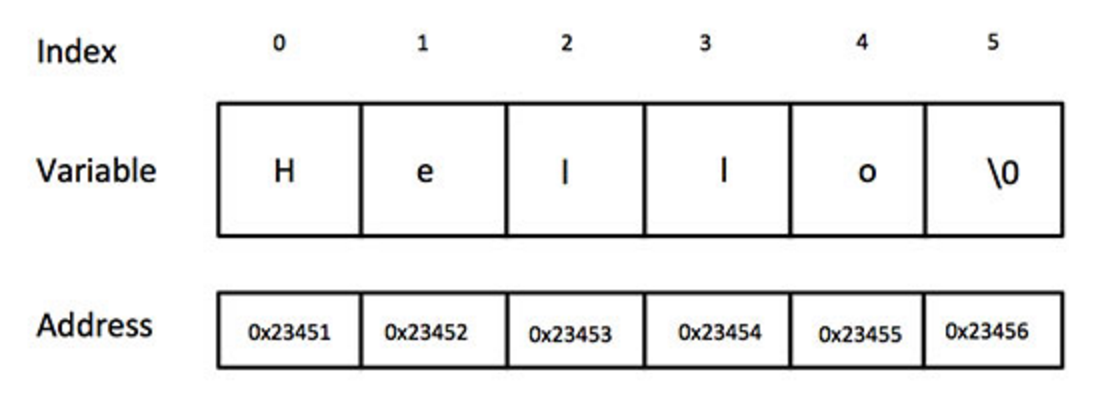
\includegraphics[width=13cm]{01/string-in-c}
\captionof{figure}{Łańcuchy znaków w C}
\end{center}

Istnieje biblioteka string.h która zawiera funkcja ułatwiające manipulowanie łańcuchami znaków.
\begin{lstlisting}[language=c]
strcpy(s1, s2); 
/*Copies string s2 into string s1*/

strcat(s1, s2);
/*Concatenates string s2 onto the end of string s1*/

strlen(s1);
/*Returns the length of string s1*/

strcmp(s1, s2);
/*Returns 0 if s1 and s2 are the same;
  less than 0 if s1<s2;
  greater than 0 if s1>s2*/
\end{lstlisting}

% 2 ---------------------------------------------------------------------------------------------------------------

\section{IT1A\_W03,IT1A\_U03,IT1A\_U07}
\textbf{Co mozesz powiedzieć o poniższej deklaracji?}
\begin{lstlisting}[language=c]
int t[10]={1, 2, [4]=1}
\end{lstlisting}

\subsection{Wprowadzenie teoretyczne}
W standardzie C99 dodane zostało takie cos jak Designated Initializers. Pozwalaja one inicjalizowac elementy tablicy w dowolnej kolejnosci podając je podczas inicjalizacji w sposób \textbf{\textit{[index]=wartosc}} lub \textbf{\textit{[poczatek ... koniec]=wartosc}}. Jeśli po inicjalizacji elementu w jeden z wymienionych powyżej sposobów pojawi się normalna inicjalizacja np {[2]=5, 4} to indeksem liczby 4 będzie 3 ponieważ przyjmie ona następny wolny indeks w tablicy, tutaj było to 3.

\begin{lstlisting}[language=c]
int tab[]={1,2,3,[4]=4,5}  /* stworzy tablice: 1,2,3,0,4,5 */
int tab[]={[1 ... 2]=5, 1} /* stworzy tablice: 0,5,5,1 */
\end{lstlisting}
	
A co jeśli zrobimy tak:
\begin{lstlisting}[language=c]
int tab[]={1,2,3,[4]=4,{5, 6, 7, 8}}
\end{lstlisting}

\textbf{\textit{Odpowiedź}}: Kod dalej sie poprawnie skompiluje a tablica bedzie miala zawartosc 1,2,3,0,4,5 (zostala wzięta 1 wartosc z bloku {5,6,7,8}) wygenerowany zostanie jedynie warning.\\
	
PS: W konstrukcji: [poczatek ... koniec]=wartosc ważna jest spacja po "poczatek"  $\ddot\smile$\\
	
Źródło: \href{https://gcc.gnu.org/onlinedocs/gcc/Designated-Inits.html}{https://gcc.gnu.org/onlinedocs/gcc/Designated-Inits.html}

\subsection{Kod testowy}
\begin{lstlisting}[language=c]
int tab[]={1,2,3,[4]=4,{5, 6, 7, 8}};

int i=0;
for(i=0; i<10; i++) {
	printf("tab[%d]=%d\n", i, tab[i]);
}
	
return 0;
\end{lstlisting}
% 3 ---------------------------------------------------------------------------------------------------------------

\section{IT1A\_W03,IT1A\_U03,IT1A\_U07} 
\textbf{W jaki sposób obliczyć długość tablicy w funkcji foo()?}
\begin{lstlisting}[language=c]
void foo(double t[]){
   // dlugosc tablicy t?
}
\end{lstlisting}

\subsection{Odpowiedź}
\begin{itemize}
\item W tym wypadku nie jest możliwe obliczenie długości tablicy.\\
\end{itemize}

\subsection{Wprowadzenie teoretyczne}
Nie jest możliwe obliczenie długości tablicy posiadając jedynie wskaźnik do niej.\\
Kompilator języka C potrafi obliczyć długość tablicy jeżeli została ona zadeklarowana w tej samej metodzie w której chcemy sprawdzić długość tablicy:
\begin{lstlisting}[language=c]
int array[] = { 1, 2, 3, 4 };
int n = sizeof(array) / sizeof(array[0]);
printf("%d", n); /* it should returns 4 */

foo(array);
/*...*/
void foo(int t[]){
   int n = sizeof(t) / sizeof(t[0]);
   printf("%d", n); /* it shouldn't returns 4 */
}
\end{lstlisting}

% 4 ---------------------------------------------------------------------------------------------------------------

\section{IT1A\_W03,IT1A\_U03,IT1A\_U07}
\textbf{Która z implementacji funkcji zwracajacej tablice jest poprawna?}

\subsection{Wprowadzenie teoretyczne}

Pamięć w C możemy alokować jedną z 3 funkcji:
\begin{lstlisting}[language=c]
void* malloc(size_t size) /* Alokuje podana 
	ilosc pamieci i nie inicjalizuje jej */
void* calloc(size_t numOfElems, size_t sizeOfElem) /* Dziala podobnie jak 
	malloc z tym, ze inicjalizuje pamiec zerami */
void* realloc(void* memory, size_t newSize) /* Realokuje pamiec moze ja 
	zwiekszyc/zmniejszyc jesli zamiast parametru memory podamy NULL
	dziala jak malloc */
\end{lstlisting}

Pamięć zwalniamy funkcją:
\begin{lstlisting}[language=c]
void free(void* memory);
\end{lstlisting}

Bonus: Dodatkowo alokacje tablicy 2D.
	
\subsection{Przykładowy kod i odpowiedzi}
	
\begin{lstlisting}[language=c]
int *tab1=getTableRealloc(10);
int *tab2;
allocTable(&tab2, 10);
int **tab2d=get2dTable(3,3);

int i=0;
for(i=0; i<10; i++) {
	tab1[i]=i;
	tab2[i]=i;
	printf("tab1[%d]=%d,tab2[%d]=%d\n", i, tab1[i], i, tab2[i]);
}
	
free(tab1);
free(tab2);
free2d(tab2d, 3);

return 0;
}

int* getTable(int n) {
	return (int*)malloc(n*sizeof(int));
}

int* getTableCalloc(int n) {
	return (int*)calloc(n, sizeof(n));
}

int* getTableRealloc(int n) {
	return (int*)realloc(NULL, n*sizeof(int));
}

void allocTable(int **tab, int n) {
	*tab=(int*)malloc(n*sizeof(int));
}

int ** get2dTable(int row, int col) {
	int **tab=(int**)malloc(row*sizeof(int));
	int i=0;
	for(i=0; i<row; i++) tab[i]=(int*)malloc(col*sizeof(int));

	return tab;
}

void free2d(int **tab, int row) {
	int i=0;
	for(i=0; i<row; i++) free(tab[i]);
	free(tab);
}
\end{lstlisting}
% 5 ---------------------------------------------------------------------------------------------------------------

\section{IT1A\_W03,IT1A\_U03,IT1A\_U07}
\textbf{Zakładając, ze wielkość typu char to jeden bajt, short to dwa bajty, a double to osiem bajtów, jaka jest wartość wyrażenia sizeof(x), gdzie x jest zmienną poniższego typu strukturalnego, dla standardowych ustawień kompilatora 32-bitowego?}
\begin{lstlisting}[language=c]
struct {
   char c;
   short i;
   double d;
} x;
\end{lstlisting}

\subsection{Wstęp teoretyczny}
W języku C każdy typ, oprócz char jest dopasowywany odpowiednio w przestrzeni adresowej.
\begin{itemize}
\item char może mieć początek na każdym bajcie w przestrzeni adresowej
\item short musi mieć początek na adresie parzystym
\item int lub float musi mieć początek na adresie podzielnym przez 4
\item long musi mieć początek na adresie podzielnym przez 8
\end{itemize}
\textbf{Przykład ułożenia zmiennych w pamięci: }
\begin{lstlisting}[language=c]
char *p;
char c;
int x;
\end{lstlisting}
Przestrzeń dla p zajmuje 4 bajty, zaraz po nim mamy chara 1 bajtowego. Ale rozmieszczenie 4-bajtowego x wymaga dodania luki:

\begin{lstlisting}[language=c]
char *p;      /* 4 or 8 bytes */
char c;       /* 1 byte */
char pad[3];  /* 3 bytes */
int x;        /* 4 bytes */
\end{lstlisting}
pad[3] reprezentuje fakt, że int musi zacząć się na adresie wielokrotności 4. \\\\
\textbf{Pierwszy przykład dla struktur (maszyna 64-bitowa)}
\begin{lstlisting}[language=c]
struct foo1 {
   char *p;     /* 8 bytes */
   char c;      /* 1 byte
   char pad[7]; /* 7 bytes */
   long x;      /* 8 bytes */
};
\end{lstlisting}
\textbf{Drugi przykład dla struktur}
\begin{lstlisting}[language=c]
struct MixedData      /* After compilation in 32-bit x86 machine */
{
    char Data1;       /* 1 byte */
    char Padding1[1]; /* 1 byte for the following 'short'
	                to be aligned on a 2 byte boundary assuming that
	                the address where structure begins is an even number */
    short Data2;      /* 2 bytes */
    int Data3;        /* 4 bytes - largest structure member */
    char Data4;       /* 1 byte */
    char Padding2[3]; /* 3 bytes to make total size of the structure 12 bytes */
};
\end{lstlisting}
Wydawać by się mogło, że sizeof(MixedData) = 9. Jednak nie - rozmiar struktury wynosi 12 bajtów! Do ostatniego elementu struktury dodany jest padding, dzięki któremu rozmiar struktury będzie wielokrotnością największego elementu struktury (tutaj int - 4 bajty).

\subsection{Odpowiedź na pytanie} 
sizeof(x) = 1 + padding(1) + 2 + padding(4) + 8 = 16 

% 6 ---------------------------------------------------------------------------------------------------------------

\section{IT1A\_W03,IT1A\_U03,IT1A\_U07}
\textbf{Przeanalizuj ponizsza deklaracje. Jakie wartosci wyrazen, w których wystepuja wskazniki p1 i p2 zostana wydrukowane? (Załóz, ze uzywasz 32-bitowego kompilatora.)}
\begin{lstlisting}[language=c]
int t[10];
int *p1=&t[0];
int *p2=&t[8];
\end{lstlisting}

\subsection{Wstęp teoretyczny}

Tablica to tak naprawdę wskaźnik na blok pamięci, dlatego możemy zrobić tak:
\begin{lstlisting}[language=c]
int tab[10];
int *tab2=tab;
\end{lstlisting}

Notacja t[x] to nic innego niż skrót na *(t+x), jak już wiemy t jest wskaźnikiem, a dodanie liczby do wskaźnika to przesunięcie wskazywanego miejsca o wielkość wskazywanego typu(np. jesli wskazuje na typ int to +1 przesunie go o sizeof(int))\\

Tutaj podam kilka zalezności które są prawdziwe:\\
Dla danych:
\begin{lstlisting}[language=c]
int t[10];
int *tmp=t;
int *p1=&t[0];
int *p2=&t[8];
\end{lstlisting}

Prawdziwe jest:
\begin{lstlisting}[language=c]
t==&t[0]
p1==t
p2==(t+8)
p2==(p1+8)
\end{lstlisting}

itp. itd.\\

p1 jest wskaźnikiem na tablicę a p2 wskaźnikiem na 8 element tablicy.

\subsection{Przykładowy kod}

\begin{lstlisting}[language=c]
int t[10];
int *tmp=t;
int *p1=&t[0];
int *p2=&t[8];

printf("t==&t[0]?:%d\n", t==&t[0]);
printf("p1==t?:%d\n", p1==t);
printf("p2==t+8?:%d\n", p2==(t+8));
printf("p2==p1+8?:%d\n", p2==(p1+8));
\end{lstlisting}

% 7 ---------------------------------------------------------------------------------------------------------------

\section{IT1A\_W03,IT1A\_U03,IT1A\_U07} 
\textbf{Przeanalizuj poniższą deklarację w języku C}
\begin{lstlisting}[language=c]
int (*x)(int, int);
\end{lstlisting}

\subsection{Odpowiedź}
\begin{itemize}
\item Deklaracja wskaźnika na funkcję przyjmującą jako parametr dwa integery\\
\end{itemize}

\subsection{Wprowadzenie teoretyczne}
\textbf{Wskaźniki na funkcje}\\
Każda funkcja tak jak i zmienna ma swoje miejsce w pamięci do którego można przypisać wskaźnik.\\
Wskaźnik na funkcje różni się od wskaźników na zmienne deklaracją:
\begin{lstlisting}[language=c]
typ_zwracanej_wartosci (*nazwa_wskaznika)(typ1 argument1, typ2 argument2, ...);
\end{lstlisting}
Przypisując nazwę funkcji bez nawiasów do wskaźnika automatycznie informujemy kompilator, że chodzi nam o adres funkcji.\\
Wskaźnika używamy tak, jak normalnej funkcji, na którą on wskazuje.\\
Przykład:
\begin{lstlisting}[language=c]
#include <stdio.h>

int suma (int lhs, int rhs){
   return lhs+rhs;
}
 
int main (){
   int (*wsk_suma)(int a, int b);
   wsk_suma = suma;
   printf("4+5=%d\n", wsk_suma(4,5));
   return 0;
}
\end{lstlisting}

% 8 ---------------------------------------------------------------------------------------------------------------
\section{IT1A\_W03,IT1A\_U03,IT1A\_U07} 
\textbf{Które stwierdzenia dotyczace operatorów w jezyku C/C++ sa poprawne:}

\subsection{Wprowadzenie teoretyczne}
Chyba wszycy wiemy jak dziala pre i post inkrementacja, ale dla zasady
zakladamy ze z zawsze jest rowne 0;
\begin{lstlisting}[language=c]
y=++z    /* y=1 z=1 */
y=z++    /* y=0 z=1 */
\end{lstlisting}

Operatory += -= itp.:
\begin{lstlisting}[language=c]
z=0; y=0;
y=z+=2;
y==2 && z==2 /* true */
\end{lstlisting}

Działania jednoargumentowe:
\begin{lstlisting}[language=c]
z=1;
-z==-1  /* true, ale po tej operacji z dalej jest rowne 1 */
+z==1   /* true ten operator tak naprawde nic nie zmienia,
	bo nawet dla z=-1 otrzymamy -1, bo +(-1)==-1 */
\end{lstlisting}

\subsection{Przykładowy kod}

\begin{lstlisting}[language=c]
int z=1;
int y=1;

printf("z==++z?: %d\n", z==++z);
printf("z!=z++?: %d\n", z==z++);
z=0; y=0;
y=z+=2;
printf("z=0 y=0, y=z+=2, y==2 z==2?: %d\n", y==2 && z==2);
z=1;
printf("z=1,-z==-1:%d\n", -z == -1);
printf("-z=%d\n", z);
\end{lstlisting}

% 9 ---------------------------------------------------------------------------------------------------------------
\section{IT1A\_W03,IT1A\_U03,IT1A\_U07} 
\textbf{Które stwierdzenia dotyczące modyfikatora static w języku C/C++ są poprawne}

\begin{itemize}
\item Zmienne lokalne

Modyfikator static sprawia, że obiekt w danej funkcji jest umieszczany w tej samej pamięci, co zmienna globalna i nie jest usuwany wraz z zakończeniem funkcji.
\begin{lstlisting}[language=c]
int licznik() {
  static int a;
  a++;
  return a;
}

int main() {
  printf("%d", licznik());  /* wypisze sie 1 */
  printf("%d", licznik());  /* wypisze sie 2 */ 
}
\end{lstlisting}

Zmienne lokalne statyczne są automatycznie inicjalizowane wartością 0.

\item Pola klasy

Statyczne pole klasy jest tworzone tylko raz, w tym samym obszarze co zmienne globalne i cały czas pamięta swoją ostatnią wartość. Jest tworzone zanim zostanie utworzony pierwszy obiekt danej klasy, zazwyczaj - tworzone są już na samym starcie programu
Pole statyczne klasy pamięta swoją wartość pomiędzy obiektami. Nie ważne z jakiego obiektu się do niego odwołasz, wartość będzie ta sama, wspólna dla wszystkich obiektów.

\item Metody

Metody statyczne - można wywołać bez podawania jakiegokolwiek obiektu. Ma to jednak swoją cenę - metody statyczne mają dostęp jedynie do innych zmiennych statycznych i metod statycznych tej klasy. 

\begin{lstlisting}[language=c]
class przyklad {
  private:
    int a, b;
    static int c;
  public:
    static void metoda() {
      c=10; 
      // b=10;         - blad! 'b' nie jest statyczne! nie ma do niego dostepu
      // this->a = 10; - blad!! w metodach statycznych 'this' nie istnieje!!
    }
};
\end{lstlisting}
\end{itemize}

Statyczne zmienne globalne i statyczne funkcje są całkowicie niewidoczne i niedostępne dla nikogo, poza plikiem, w którym zostały zdefiniowane.

% 10 ---------------------------------------------------------------------------------------------------------------
\section{IT1A\_W03,IT1A\_U03,IT1A\_U07} 
\textbf{Dzieki konwencji wywołania funkcji w jezyku C znanej jako \_\_cdecl mozliwa jest implementacja funkcji o zmiennej liczbie argumentów, jak printf(). Które stwierdzenia charakteryzujace funkcje typu \_\_cdecl sa prawdziwe?}

\subsection{Wstęp teoretyczny}

Patrząc z perspektywy programisty C:
\begin{itemize}
\item Wymagany jest chociaz jeden normalny parametr
\item Musimy znać liczbę parametrów, np. przekazać jako normalny argument.(printf bierze ta informacje ze stringa z formatem)
\item Argumenty moga byc dowolnego typu potem wyciagamy je makrem var\_arg
\end{itemize}

Z punktu widzenia Assemblera:
\begin{itemize}
\item Stos jest czyszczony przez obiekt wywołujący, a nie przez samą funkcję dzięki czemu możemy tworzyć funkcje ze zmienną ilością parametrów ponieważ obiekt wywołujący wie ile parametrów przekazał funkcji, a sama funkcja nie ma takiej informacji.
\item Kod asemblera programu z funkcjami w konwencji \_\_cdecl jest wiekszy niż w przypadku innych konwencji ponieważ przy każdym wywołaniu funkcji na poziomie asemblera musi się znaleźć także wyczyzszczenie stosu z parametrów
\end{itemize}

Przykład konwencja stdcall(domyślna dla Win32):\\
push 5	;wrzucamy argument na stos\\
call potega	;wywołujemy funkcje\\

Przykład konwencja cdecl:\\
push 5	;wrzucamy argument na stos\\
call potega	;wywołujemy funkcje\\
add esp, 4	;sami czyścimy stos\\

Jak widać w przypadku cdecl mamy o jedną instrukcje więcej.\\

Istnieje jeszcze kilka innych konwencji wszystkie różnią się kodem assemblera.\\

Jak wybrać ręcznie konwencję dla funkcji?\\
\begin{lstlisting}[language=c]
int __cdecl suma(int n, ...);
int __stdcall suma(int a, ...);  /* Zapytacie jak to moze dzialac jak napisalem, 
	ze tutaj funkcja sama czysci argumenty :D, 
	Odpowiedz to: kompilator czaruje i generuje funkcje vararg w _cdecl */
\end{lstlisting}

Źródło: \href{http://www.p-programowanie.pl/cpp/konwencje-wywolywania-funkcji/}{http://www.p-programowanie.pl/cpp/konwencje-wywolywania-funkcji/}

\subsection{Przykładowy kod}

\begin{lstlisting}[language=c]
printf("sum=%d\n", sum(4, 1, 2, 3, 4));

int __cdecl sum(int n, ...) {
	va_list ap;
	va_start(ap, n);
	int i=0;
	int sum=0;
	for(i=0; i<n; i++) sum+=va_arg(ap, int);
	va_end(ap);
	
	return sum;
}
\end{lstlisting}

% 11 ---------------------------------------------------------------------------------------------------------------

\section{IT1A\_W03,IT1A\_U03,IT1A\_U07} 
\textbf{W jaki sposób przekazywany jest parametr do będący tablicą do funkcji w języku C?}
\begin{lstlisting}[language=c]
int main(int argc, char* argv[]){
   //...
}
\end{lstlisting}

\subsection{Odpowiedź}
\begin{itemize}
\item Na stos jest przekazywany adres pierwszego elementu tablicy\\
\end{itemize}

\subsection{Wprowadzenie teoretyczne}
Tablice są przekazywane do funkcji zawsze jako wskaźnik.\\
Zwykłe zmienne oraz obiekty(struktury) mogą być przekazywane przez wartość lub przez referencję.
\begin{itemize}
\item Przez wartość - na stos trafia kopia danej zmiennej lub obiektu.\\
Jeżeli wewnątrz struktury przekazywanej przez wartość znajduje się wskaźnik (lub tablica) to zostanie skopiowany wskaźnik. W skutek czego oryginał i kopia będą współdzielić jeden wskaźnik / tablicę. Zmieniając coś w kopii paramteru nie zmieniamy jego pierwowzoru.
\item Przez referencję - na stos trafia kopia adresu przesyłanego paramteru. Zmieniając coś w referencji, zmieniamy oryginał.
\end{itemize}

% 12 ---------------------------------------------------------------------------------------------------------------
\section{IT1A\_W03,IT1A\_U03,IT1A\_U07} 
\textbf{Które stwierdzenia odnoszace sie do przydziału pamieci dla zmiennych w jezykach C i C++ sa prawdziwe?}

\subsection{Wprowadzenie teoretyczne}

\begin{itemize}
\item Zmienne statyczne, automatyczne (zmienne globalne, statyczne, lokalne, niealokowane) przechowywane są na stosie
\item Zmienne dynamiczne (alokowane poprzez malloc, new, itp.) przechowywane są na stercie
\item Sterta jest wspólna dla wszytkich programów
\item Stos jest ograniczony co do rozmiaru, co za tym idzie nie można na stosie zaalokowac dużej ilości pamięci należy to zrobić dynamicznie na stercie (to jest ta jedna z mistycznych sytuacji kiedy malloc zwraca null'a)
\end{itemize}

% 13 ---------------------------------------------------------------------------------------------------------------

\section{IT1A\_W04,IT1A\_U04,IT1A\_U21} 
\textbf{Które ze stwierdzeń, odnoszących się do referencji w języku C++ są poprawne?}

\subsection{Wprowadzenie teoretyczne}
Referencja w swym działaniu przypomina wskaźniki. Różnica polega jednak na tym, że do referencji można przypisać adres tylko raz ( w momencie deklaracji ), a jej dalsze używanie niczym się nie różni od używania zwykłej zmiennej. Operacje jakie wykona się na zmiennej referencyjnej, zostaną odzwierciedlone na zmiennej zwykłej, z której pobrano adres.\\
Przykład użycia:
\begin{lstlisting}[language=c]
int i = 0;
int &ref_i = i;
cout << i;      // wypisze 0
ref_i = 1;
cout << i;      // wypisze 1
cout << ref_i;  // wypisze 1
\end{lstlisting}
Różnice między wskaźnikami i referencjami:
\begin{lstlisting}[language=c]
int a,b;
int *wsk_a = &a, *wsk_b = &b;
int &ref_a = a, &ref_b = b;
int &ref_c; // kompilator nie zezwoli na to - referencja niezainicjalizowana

wsk_b = &a; // ok
ref_b = &a; // tak sie nie da
\end{lstlisting}
W C++ można było przekazywać parametry do funkcji przez referencję w podobny sposób jak w C. W C++ jednak używa się referencji w o wiele prostszy sposób ( tak jak zwykły parametr ).

\begin{lstlisting}[language=c]
void zwieksz_c (int *i){
   ++(*i); // ta funkcja jest napisana w stylu C
}
void zwieksz_cpp (int& i){
   ++i;    // ta funkcja wykorzystuje mozliwosci C++
}

// wywolanie funkcji niczym sie nie rozni.
int i = 10;
zwieksz_c(&i);
zwieksz_cpp(&i);
\end{lstlisting}

% 14 ---------------------------------------------------------------------------------------------------------------
\section{IT1A\_W04,IT1A\_U04,IT1A\_U07,IT1A\_U21} 
\textbf{Jezeli podczas wykonania instrukcji w C++:}
\begin{lstlisting}[language=c]
A* ptr = new A();
\end{lstlisting}
\textbf{wygenerowany został wyjatek, jego przyczyna moze byc nastepujaca:}

\subsection{Odpowiedź}
Przychodzą mi do głowy 2 możliwości:
\begin{itemize}
\item W konstuktorze wyrzucany jest wyjątek
\item Brakuje pamięci wtedy mechanizm C++ rzuca wyjątkiem std::bad\_alloc
\end{itemize}

\subsection{Przykładowy kod}
\begin{lstlisting}[language=c]
class Exception {
	
};

class A {
	private:
		int i;
	public:
		A(bool a=false) {
			if(a) throw Exception();
		}
		
		~A() {
			cout << "Descruting-A" << endl;
		}
		
		int getI(void) {
			return i;
		}
		void setI(int i) {
			this->i=i;
		}
};

int main(int argc, char** argv) {
	A *a=NULL;
	try {
		A b;
		a=new A(true);
	} catch(Exception& e) {
		cout << "Exception" << endl;
		if(a==NULL) cout << "a-is-null" << endl;
	}
//	if(a==NULL) cout << "a-is-null";
//	a->setI(10);
//	cout << "Wartosc: " << a->getI() << endl;

	delete a;
	
	return 0;
}

\end{lstlisting}

% 15 ---------------------------------------------------------------------------------------------------------------
\section{IT1A\_W04,IT1A\_U04,IT1A\_U07,IT1A\_U21} 
\textbf{Przeanalizuj fragment kodu w języku C++, w którym pojawia się wywołanie operatora <<:}
\begin{lstlisting}[language=c]
A a;
std::cout<<a;
\end{lstlisting}
Która z podanych implementacji operatora << jest poprawna (przykładowy kod zostanie skompilowany i wykonany)?

\subsection{Wstęp teoretyczny}
Aby przeładować operator << musimy zdefiniować funkcję o prototypie: 
\begin{lstlisting}[language=c]
ostream& operator<<(ostream&, const Klasa&);
\end{lstlisting}
Jeśli przy wypisywaniu informacji o obiekcie potrzebny jest dostęp do prywatnych lub chronionych składowych, to funkcję tę należy też zadeklarować jako zaprzyjaźnioną wewnątrz klasy:
\begin{lstlisting}[language=c]
class Klasa {
  public:
   friend ostream& operator<<(ostream&, const Klasa&);
};
\end{lstlisting}
Przykład implementacji funkcji:
\begin{lstlisting}[language=c]
ostream& operator<<(ostream& str, const Klasa& k) {
   return str << k.nazwa << " (" << k.nazwa2 << ")";
}
\end{lstlisting}
\subsection{Odpowiedź}
Według odpowiedzi z egzaminu 2011, poprawne były odpowiedzi dwie, w których operator był w osobnej funkcji

% 16 ---------------------------------------------------------------------------------------------------------------
\section{IT1A\_W04,IT1A\_U04,IT1A\_U07,IT1A\_U21} 
\textbf{Zdefiniowano szablon (wzorzec) funkcji}
\begin{lstlisting}[language=c]
template<class T>
T suma( T* table, int size)
{
	T t=T();
	for(int i=0; i<size; i++) t+=table[i];
	return t;
}
\end{lstlisting}
\textbf{Proces instancjacji szablonu polega na zastapieniu typów i zmiennych bedacych parametrami szablonu konkretnymi typami i wartosciami, a nastepnie generacji kodu wynikowego. Jakie załozenia musi spełniac typ T, aby instancjacja szablonu była mozliwa?}
\\
Zeby mozna było wywołac szablon funkcji parametrem może być:
\begin{itemize}
\item typ prosty
\item klasa która posiada domyślny konstruktor oraz przeciążony oprator+=
\end{itemize}

\begin{lstlisting}[language=c]
class A {
	
	private:
		int value;
	
	public:
		
		A(int value=0) {
			this->value=value;
		}
		
		int getValue(void) {
			return value;
		}
		
		void setValue(int value) {
			this->value=value;
		}
		
		friend ostream& operator<<(ostream& out, A const& obj) {
			out << obj.value;
		}
		
		A operator+(A const& obj) {
			return A(value+obj.value);
		}
		
		A& operator+=(A const& obj) {
			value+=obj.value;
		}
};

template<class T>
T sum(T arg1, T arg2) {
	return arg1+arg2;
}

template<class T>
T suma(T *table, int size) {
	T t=T();
	for(int i=0; i<size;i++) t+=table[i];
	return t;
}

int main(int argc, char** argv) {
	A a(5),b(3);
	A tab[]={A(1), A(2), A(3), A(4)};
	
	
	cout << "Suma tablicy: " << suma(tab, 4) << endl;
	
	cout << sum(a, b) << endl;
	cout << a << "+" << b << endl;
	
	cout << sum(1, 2) << " " << sum(1.0, 1.1) << endl;
	
	return 0;
}
\end{lstlisting}

% 17 ---------------------------------------------------------------------------------------------------------------
\section{IT1A\_W04,IT1A\_U04,IT1A\_U07,IT1A\_U21} 
\textbf{Klasa B przechowuje wskaźniki do obiektów klasy A w kontenerze vector standardowej biblioteki C++ (STL)}
\begin{lstlisting}[language=c]
class A{...};
class B{
   public:
   std::vector<A*> v;
   void add(A &a) { v.push_back(new A(a));}
   ~B();
}
\end{lstlisting}
\textbf{Która z implementacji destruktora jest poprawna ( kompiluje się, nie prowadzi do błędów wykonania lub wycieków pamięci)?}

\subsection{Odpowiedź}
\begin{itemize}
\item 
\begin{lstlisting}[language=c]
 B::~B(){
    for ( std::vector<A*>::iterator i = v.begin(); i != v.end(); ++i )
       delete *i; // wywolujemy delete na obiekcie, nie na wskazniku do niego!
 }
\end{lstlisting}
\end{itemize}

\subsection{Wprowadzenie teoretyczne}
Dla każdego elementu w wektorze powinien zostać, wywołany operator delete. W szczególności używanie funkcji typu std::erase czy std::remove (i ich wariantów, typu std::remove\_if), czyszczenie pojemnika, itp. same nie dają poprawnego rozwiązania – na elementach musi byd jawnie wywołany operator delete, bo żadna z takich funkcji tego sama nie robi. Jeżeli mamy do czynienia z kontenerem obiektów ( czyli nie przechowujemy danych prymitywnych np. char lub wskaźników ) to możemy wywołać funkcję std::vector<T>::clear() która wywoła na każdym obiekcie operację delete.

% 18 ---------------------------------------------------------------------------------------------------------------

\section{IT1A\_W04,IT1A\_U04,IT1A\_U07,IT1A\_U21}
\textbf{Szablon set<T> zdefiniowany w standardowej bibliotece C++ (STL) przechowuje elementy w drzewiastych strukturach danych. Który z przedstawionych typów danych moze byc zastosowany jako parametr instancjacji szablonu set<T>? }

\subsection{Odpowiedź}
Każdy typ, który ma przeładowany operator < lub jeśli podamy przy tworzeniu kolekcji własny komperator
\textbf{set<Typ, Komperator> kolekcja;}

Komperator ma postać:
\begin{lstlisting}[language=c]
struct CustomComperator {
	bool operator()(A const& lhs, A const& rhs) const {
		return lhs.getValue()<rhs.getValue();
	}
};
\end{lstlisting}

\subsection{Przykładowy kod}
\begin{lstlisting}[language=c]
class A {
	
	private:
		int value;
	
	public:
		
		A(int value=0) {
			this->value=value;
		}
		
		int getValue(void) const {
			return value;
		}
		
		void setValue(int value) {
			this->value=value;
		}
		
		friend ostream& operator<<(ostream& out, A const& obj) {
			out << obj.value;
		}
		
		A operator+(A const& obj) const {
			return A(value+obj.value);
		}
		
		A& operator+=(A const& obj) {
			value+=obj.value;
		}
		
		bool operator<(A const& obj) const {
			return value<obj.value;
		}
};

struct CustomComperator {
	bool operator()(A const& lhs, A const& rhs) const {
		return lhs.getValue()<rhs.getValue();
	}
};

int main(int argc, char** argv) {
	
//	set<A, CustomComperator> mapa;
	set<A> mapa;
	
	mapa.insert(A(4));
	mapa.insert(A(2));
	mapa.insert(A(1));
	
	for(set<A>::iterator it=mapa.begin(); it!=mapa.end(); ++it) {
		cout << *it << endl;
	}
	
	return 0;
}
\end{lstlisting}

% 19 ---------------------------------------------------------------------------------------------------------------

\section{IT1A\_W04,IT1A\_U04,IT1A\_U07,IT1A\_U21}
\textbf{Które ze stwierdzeń odnoszących się do konstruktorów kopiujących i operatorów przypisania w języku C++ są poprawne?}

\subsection{Wprowadzenie teoretyczne}
\begin{itemize}
\item Publiczny konstruktor kopiujący oraz operator przypisania zostaną automatycznie wygenerowane przez kompilator, jeśli programista je pominie.
\item Zarówno automatycznie wygenerowany konstruktor kopiujący, jak i operator przypisania kopiują obiekty bit po bicie.
\item Inicjalizacja (tworzenie obiektu na zasadzie: X x = y;) wywołuje konstruktor kopiujący, nie operator przypisania.
\item Oprócz inicjalizacji, konstruktor kopiujący wywoływany jest gdy przekazuje się lub zwraca obiekty przez wartośd (trzeba zrobid kopię obiektu).
\item W niektórych przypadkach, jeśli kompilator jest sprytny i zrobi np. optymalizację wartości zwracanej, to konstruktor kopiujący może nie zostać wywołany przy wywołaniu funkcji zwracającej obiekt przez wartośd.
\end{itemize}

% 20 ---------------------------------------------------------------------------------------------------------------

\section{IT1A\_W04,IT1A\_U04,IT1A\_U07,IT1A\_U21}
\textbf{Implementacja przeciazonych operatorów C++ powinna odzwierciedlac semantyke operacji na typach wbudowanych. Biorac pod uwage to wymaganie, które z implementacji operatorów dla klasy X zadeklarowanej ponizej jest poprawna? }
\begin{lstlisting}[language=c]
class X
{
friend X&operator+=(X&a, const X&b);
	int x;
public:
	X(int _x=0):x(_x) {}
	X&operator+(const X&o);
	X&operator++(int);
	X&operator-=(const X&o);
};
\end{lstlisting}

\subsection{Wprowadzenie teoretyczne}

Operatory można przeciążać na 2 sposoby:
\begin{itemize}
	\item definiując je jako metodę klasy
	\item definiując je jako funkcję zewnętrzną poza klasą
\end{itemize}
	
Dla przykładu przeładowanie operatora "+":\\
W klasie:\\
- zwracany\_typ operator+(const typ\_\&) const;\\
Poza klasą:\\
- zwracany\_typ operator+(const typ1\&, const typ2\&);\\

Dla operatorów 1 argumentowych na przykładzie ++:\\
W klasie:\\
- zwracany\_typ\& operator++();\\
Poza klasą:\\
- zwracany\_typ\& operator++(typ\&);\\

Teraz pewnie zadajecie sobie pytanie dobra no, ale jak to jest z tymi const. \\
Jest to dość intuicyjne i trzeba się trzymać kilku zasad:
\begin{itemize}
	\item jeśli NIE zmieniamy jakiegoś parametru to dajemy przy nim const
	\item jeśli przeładowujemy w klasie i operator nie zmienia klasy tylko zwraca nowy obiekt to na metodzie dajemy na koncu const
\end{itemize}

Dodatkowe pseudo reguły:
\begin{itemize}
	\item zazwyczaj wszytko przekazujemy jako referencję(\&) chyba że zwracamy nowy obiekt tak jak jest to w przypadku np. operatora +
	\item operator można zdefiniować jako funkcje zaprzyjaźnioną żeby mieć dostęp z zewnątrz do prywatnych pól klasy trzeba tak zrobic np. w przypadku operatora wypisania, np.:
		\begin{lstlisting}[language=c]
	friend ostream& operator<< (ostream&,Foo const&);
		\end{lstlisting}
	\end{itemize}
	
Żywy przyklad mozna zobaczyc tutaj na klasie A.\\

Co do przykladu z pytan:\\
\begin{lstlisting}[language=c]
class X
{
	friend X& operator+=(X &a, const X& b); /* Dobrze */
	int x;
	public:
		X(int _x = 0) : x(_x) { }
		X& operator+(const X&o);  /* Zle cala metoda powinna byc const */
		X& operator++(int);       /* Dobrze, int i tak bedzie kopia w funkcji */
		X& operator-=(const X&o); /* Dobrze */
};
\end{lstlisting}

\subsection{Przykładowy kod}
\begin{lstlisting}[language=c]
class A {
	
	private:
		int value;
	
	public:
		
		A(int value=0) {
			this->value=value;
		}
		
		int getValue(void) const {
			return value;
		}
		
		void setValue(int value) {
			this->value=value;
		}
		
		friend ostream& operator<<(ostream& out, A const& obj) {
			out << obj.value;
		}
		
		A operator+(A const& obj) const {
			return A(value+obj.value);
		}
		
		A& operator+=(A const& obj) {
			value+=obj.value;
		}
		
		bool operator<(A const& obj) const {
			return value<obj.value;
		}
};

int main(int argc, char** argv) {
	
	cout << A(1) << endl;
	
	return 0;
}
\end{lstlisting}

% 21 ---------------------------------------------------------------------------------------------------------------

\section{IT1A\_W04,IT1A\_U04,IT1A\_U07,IT1A\_U21}
\textbf{W języku C++ dostep do informacji o typie obiektu w trakcie wykonania programu umożliwają następujące operatory:}

\subsection{Odpowiedź}
\begin{itemize}
\item typeid
\end{itemize}

\subsection{Wprowadzenie teoretyczne}
typeid jest funkcją która zwraca obiekt klasy std::type\_info lub wyrzucającą obiekt klasy std::bad\_typeid w przypadku gdy używamy tej funkcji z nullową wartością.\\
Przykład:
\begin{lstlisting}[language=c]
#include <iostream>
#include <typeinfo>  //for 'typeid' to work

class Person {
public:
   // ... Person members ...
   virtual ~Person() {}
};

class Employee : public Person {
   // ... Employee members ...
};

int main () {
   Person person;
   Employee employee;
   Person *ptr = &employee;
   // The string returned by typeid::name is implementation-defined
   
   std::cout << typeid(person).name() << std::endl;   // Person
   std::cout << typeid(employee).name() << std::endl; // Employee
   std::cout << typeid(ptr).name() << std::endl;      // Person * 
   std::cout << typeid(*ptr).name() << std::endl;     // Employee
}
\end{lstlisting}

% 22 ---------------------------------------------------------------------------------------------------------------

\section{IT1A\_W04,IT1A\_U04,IT1A\_U07,IT1A\_U21}
\textbf{Zadeklarowano dwie klasy w nastepujacy sposób:}
\begin{lstlisting}[language=c]
class A{
public:
	virtual void f(){printf("VA ");}
	void g(){printf("A ");}
};

class B: public A{
public:
	void f(){printf("VB ");}
	void g(){printf("B ");}
};
\end{lstlisting}
\textbf{oraz utworzono dwa obiekty:}
\begin{lstlisting}[language=c]
A* a1 = new A();
A* a2 = new B();
\end{lstlisting}

\subsection{Wprowadzenie teoretyczne}
Wywołanie metody f na obu obiektach spowoduje wywołanie odpowiednich implementacji danej metody, poniewaz jest ona oznaczona jako wirtualna,
czyli wypisze się "VA VB".\\

Natomiast wywołanie metody g spowoduje wywołanie jedynie implementacji wypisującej "A ", ponieważ metoda nie jest wirtualna, a typ wskaźnika to A, czyli wywołanie:
\begin{lstlisting}[language=c]
a1->g();
a2->g();
\end{lstlisting}
wypisze "B B".

\textbf{Uwagi:}
\begin{itemize}
\item metody wirtualne wywoływane w konstruktorze zachowują się jak niewirtualne, czyli wywołają implementacje metody z danej klasy
\item konstruktor jest tak jakby zawsze wirtualny
\item destruktor powinien być ZAWSZE wirtualny. DLa przykłądu jeśli mamy takie dziedziczenie B dziedziczy po A to jeśli destruktor w klasie A będzie nie wierualny to nie wywoła sie destruktor klasy B - czytaj: bardzo źle :).
\end{itemize}

\subsection{Przykładowy kod}
\begin{lstlisting}[language=c]
class A {
	public:
		virtual void f() {cout << "VA ";}
		void g() {cout << "A ";}
};

class B : public A {
	public:
		void f() {cout << "VB ";}
		void g() {cout << "B ";}
};

class C : public B {
	public:
		void f() { cout << "VC "; }
};

int main(int argc, char** argv) {
	A* a1=new A();
	A* a2=new B();
	B* a3=new C();
	
	a1->f();
	a2->f();
	a3->f();
	
	cout << endl;
	
	a1->g();
	a2->g();
	
	delete a1;
	delete a2;
	
	return 0;
}
\end{lstlisting}
\chapter{Wstep do systemow uniksowych}
\PartialToc
%\startcontents[chapters]
%\printcontents[chapters]{}{1}{\section*{\contentsname}}
\vspace{0.4cm}
\noindent  

\answer
{IT1A\_U09 Podstawowa architektura Unixa obejmuje:}
{przykładowa odp.) Stos TCP/IP}
{F}
{jądro systemu, powłoki, oprogramowanie systemowe, pliki i katalogi}
{
\begin{itemize}
\item Jądro - serce systemu operacyjnego. Zapewnia interakcję ze sprzętam. Główne zadania: zarządzanie pamięcią, scheduling, zarządzanie plikami.

\item Powłoka - przetwarza żądania i polecenia wywołuje programy. Najbardziej znane powłoki w systemie Unix: C Shell, Bourne Shell and Korn Shell

\item Polecenia i komendy(oprogramowanie systemowe) - ponad 250 standardowych komend plus licznych dostarczonych przez 3rd party software. Przykłady: cp, mv, cat and grep etc.

\item Pliki i katalogi - Dane przechowywane w plikach. Wszystkie pliki są zebrane w katalogach o strukturze drzewiastej(system plików)
\end{itemize}
}
%%%%%%%%%%%%%%%%%%%%%%%%%%%%%%%%%%%%%%%%%%%%%%%%%%
\answer
{IT1A\_U09,IT1A\_W09 W systemie plików Unix:}
{pliki które zmieniają się często są w katalogu /var}
{T}
{

System plików jest logiczną strukturą organizacji plików
\begin{itemize}
\item ma strukturę drzewiastą,
\item jest zawsze tylko jedna taka struktura,
\item bezwględny początek '/' systemu plików (root),
\item inne systemy mogą być włączane jako kolejne gałęzie,
\item katalog bieżący '.', katalog nadrzędny '..',
\item wszystkie pliki i katalogi mają nazwy będące ciągami znaków alfanumerycznych,
\item nazwy mogą być długie i są case sensitive,
\item katalog rozdziela się znakiem "/",
\item ścieżka dostępu pozwala na umiejscowienie pliku w strukturze systemu,
\item pełna (bezwzględna) ścieżka określa jego położenie względem początku drzewa i zaczyna się od /, np. /etc/passwd,
\item względna ścieżka określa położenie względem katalogu bieżącego.
\end{itemize}
Ponadto:
\begin{itemize}
\item dostęp do wszystkich zasobów systemu Unix jest realizowany przez pliki,
\item plik jest wygodną abstrakcją,
\item wszystko jest plikiem,
\item pliki są reprezentowane w systemie plików przez węzły indeksowe (i-inode),
\item katalog jest szczególnym przypadkiem pliku, który zawiera listę w postaci (nazwa pliku, i-node),
\item i-node jest podstawowym elementem składowym systemu plików,
\item zawiera wszystkie informacje o pliku, poza jego nazwą (ta jest w katalogu!),
\item wskazuje na to, gdzie się fizycznie znajdują dane zawarte w pliku,
\item przechowuje daty: modyfikacji węzła ctime, modyfikacji (danych pliku mtime, dostępu do pliku atime,
\item opisuje: typ i rozmiar obiektu, wraz z liczbą dowiązań (nazw),
\item określa właściciela i grupę pliku, oraz prawa dostępu.
\end{itemize}}
{
(...)
}

%%%%%%%%%%%%%%%%%%%%%%%%%%%%%%%%%%%%%%%%%%%%%%
\answer
{ IT1A\_U09 Prawo dostępu do pliku 453 pozwala}
{Wszystkim czytać plik}
{F}
{użytkownikowi na odczyt, grupie na odczyt i uruchomienie, pozostałym na zapis
}
{Każde z praw dostępu ma swoją wartość(4 - odczyt, 2-zapis, 1- uruchomienie) nadawane kolejno dla usera, grupi i reszty. Dodawane są one do siebie i na tej podstawie ustala się prawa  }
%%%%%%%%%%%%%%%%%%%%%%%%%%%%%%%%%%%%%%%%%%%%%%
\answer
{IT1A\_U09 W systemie plików}
{pliki które zmieniają się często są w katalogu /var}
{T}
{(...)}
{Jak dwa pytania wyżej}
%%%%%%%%%%%%%%%%%%%%%%%%%%%%%%%%%%%%%%%%%%%%%%%%%%%%%%%%%%%%%%%%%%%%%%%%%%%%%%%%%%%%%%%%%%%%%
\answer
{ IT1A\_U09 Które z poniższych stwierdzeń sa prawdziwe?:}
{przykładowa odp.) każde konto musi należeć do co najmniej jednej grupy}
{"F"}
{}
{
Konto użytkownika to identyfikator <user name> oraz dołączone do niego zasoby, pliki i dane. Maksymalna  długość  identyfikatora  użytkownika  wynosi 8 znaków.
Wszystkie potrzebne informacje na temat kont użytkowników zawarte są w pliku \textit{/etc/passwd}.\\
Struktura jednego wpisu to: \\
username:x:UID:GID:GECOS:home\_dir:shell
UID – liczbowy identyfikator użytkownika \\
GID – liczbowy identyfikator grupy \\
GECOS – General Electric Comprehensive Operating System \\ 

W większości dystrybucji są narzędzia do obsługi kont (np. userconfig). Informacje o użytkownikach dostarczają polecenia: \textit{w, who, finger}
}

%%%%%%%%%%%%%%%%%%%%%%%%%%%%%%%%%%%%%%%%%%%%%%%%%%%%%%%%%%%%%%%%%%%%%%%%%%%%%%%%%%%%%%%%%%%%%
\answer
{IT1A\_W09 Przy zarządzaniu systemami plików}
{system plików sprawdzamy przez checkfs}
{F}
{poprawna komenda do sprawdzenia intergralności systemu plików to fsck}
{

Komendy zarządzania systemami plików:
\begin{itemize}
\item badblocks – kontroluje badblocks (złe bloki urządzeń)
\item df – sprawdzanie przestrzeni (również wolnej) na dyskach
\item fsck – sprawdzanie integralności systemu plików
\item fdisk – manipulacje w tabeli partycji także cfdisk, sfdisk, parted
\item mkfs – tworzenie systemu plików , 'formatowanie'
\item lvm – narzędzia do LVM (zarządzanie przestrzenią pamięci masowej)
\item mount – montowanie urządzeń/zasobów w systemie plików
\item umount – odmontowanie zasobu z systemu plików
\item dd – operacje io na dysku z pominięciem systemu plików
\end{itemize}
}

%%%%%%%%%%%%%%%%%%%%%%%%%%%%%%%%%%%%%%%%%%%%%%%%%%%%%%%%%%%%%%%%%%%%%%%%%%%%%%%%%%%%%%%%%%%%%
\answer
{ IT1A\_U09 W trakcie startu systemu Unix}
{przykładowa odp.) pierwszym tworzonym procesem jest Init}
{F}
{}
{
Procedura uruchomieniowa systemu Unix: \\
- sprzętowy program uruchomieniowy wczytuje program uruchomieniowy z dysku. Ten z kolei ładuje plik /vniunix (czasem nazwany /unix) z głównego katalogu głównego dysku. Są już w nim zawarte wszystkie programy obsługi urządzeń. Każdy z nicli sprawdza, czy odpowiednie urządzenie w systemie jest obecne i działa. Jeżeli coś jest nie w porządku, informacja o tym jest przechowywa-na na później, gdyby ktoś się odwoływał do urządzenia. Dodanie nowych urządzeń wymaga powtórnego zbudowania systemu. Zagadnienie to jest wyjątkowo obszerne i skomplikowane, ale odpowiednie informacje można znaleźć w dokumentacji własnego systemu.
\\
-następnie są uruchamiane trzy procesy. Dwa z nich zajmują się zarządzaniem pamięcią fizyczną (pagedaemon o numerze 2) i obsługą pamięci wirtualnej fswapper o numerze 0), trzeci inicjalizuje resztę systemu (init o numerze l).
-W Systemie V spis programów, które mają być uruchomione przez init, jest zawarty w pliku /etc/inittab. Programy te wykonują operacje zbli-żone do poleceń zawartych w plikach /etc/rc i /etc/rc. local. Kiedy użytkownik odpowiada na znak zachęty "login:", program getty uruchamia program login, który pobiera od użytkownika hasło i porównuje je z zawartym w pliku /etc/passwd. Jeżeli hasło się zgadza, login tworzy środowisko i wypisuje komunikat dnia (/etc/motd). Na końcu jest uruchamiany program początkowy określony przez plik /etc/passwd, zazwyczaj powłoka. Powłoka wykonuje wtedy skrypt uru-chomieniowy (na przykład .profile) i czeka na wprowadzanie poleceń. Kiedy użytkownik opuszcza powłokę, zazwyczaj za pomocą <control-D>, dowiaduje się o tym proces init i powtórnie uruchamia program getty na danym terminalu.
}

%%%%%%%%%%%%%%%%%%%%%%%%%%%%%%%%%%%%%%%%%%%
\answer
{IT1A\_W09 Procesy w systemie Unix }
{Działają dynamicznie i synchronicznie}
{T}
{"-"}
{Wykonanie instrukcji jednego procesu musi być sekwencyjne. \\
Każdy proces ma własny licznik instrukcji, który wskazuje następną instrukcję do wykonania, oraz własny obszar przydzielonej mu pamięci operacyjnej.\\
W systemie Unix nowy proces jest tworzony w wyniku wywołania przez proces macierzysty funkcji systemowej fork. Powstaje wówczas nowy proces, który jest dokładną kopią macierzystego.\\
Każdy proces ma m.in. unikatowy identyfikator- PID (ang. process identifier), który jednoznacznie określa działający proces oraz identyfikator procesu macierzystego PPID\\
Proces jest podstawową aktywną jednostką pracy zarządzaną przez system.\\
Procesy mogą być dynamicznie tworzone i usuwane. \\
Pamięć operacyjna zwykle jest podzielona na cztery części (nazywane segmentami):
\begin{itemize}
\item segment kodu -- zawiera instrukcje wykonywanego programu
\item segment danych -- zawiera zmienne globalne programu
\item stos -- jest używany do wywoływania procedur, przekazywania parametrów i wyników, oraz przechowywania zmiennych lokalnych 
\item sterta -- z tego obszaru przydzielana jest pamięć dla zmiennych dynamicznych
\end{itemize}
}

%%%%%%%%%%%%%%%%%%%%%%%%%%%%%%%%%%%%%%%%%%%%%%
\answer
{IT1A\_U09 Przykłady komunikacji międzyprocesowej w Unixie to}
{pamięc dzielona}
{T}
{
\begin{itemize}
\item sygnały
\item pliki i blokady – najprostsza i najstarsza forma IPC (Inter-Process Communication)
\item łącza nienazwane- FIFO, identyfikowane przez nazwę, istnieje jako plik, po zakończeniu procesów nie jest usuwane
\item łącza nazwane- zapisywane w deskryptorach plików, dostęp tylko przez procesy pokrewne(dziedziczenie deskryptorów), po realizacji ostatniego procesu są zamykane
\item semafory- Używane są do kontroli dostepu do zasobów systemu dzielonych przez kilka procesów, dostarczają lepsze blokady
\item kolejki komunikatów- rodzaj FIFO,Istnieje mozliwosc umieszczania komunikatow w okreslonych kolejkach (z zachowaniem kolejnosci ich wysylania przez procesy) oraz odbierania komunikatu na pare roznych sposobow (zaleznie od typu, czasu przybycia itp.).
\item pamięć dzielona- Jest to obszar pamięci dzielony pomiędzy kilkoma procesami. Dane umieszczane są przez proces w tzw. segmentach, w obszarze adresowym procesu wywołującego. Może z nich korzystać wiele procesów. Pamięć dzielona jest najszybszym sposobem komunikacji pomiędzy procesami.
\item gniazda- wykorzystywane do komunikacji przez sieć, umożliwiają komunikacje dwukierunkową, Gniazda posiadają takie właściwości jak: swój typ, lokalny adres, oraz opcjonalnie port. Typ gniazda określa sposób wymiany danych, adres IP określa węzeł w sieci a numer portu określa proces w węźle.
\end{itemize}
}
{"up"}
%%%%%%%%%%%%%%%%%%%%%%%%%%%%%%%%%%%%%%%%%%%%%%%%%%%%%%%%%%%%%%%%%%%%%%%%%%%%%%%%%%%%%%%%%%%%%
\answer
{ IT1A\_W09 Rejestrowanie zdarzeń w Unixie}
{logi mogą być porządkowane cyklicznie z użyciem Cron-a}
{T}
{"-"}
{Cron umożliwia cykliczne uruchamianie programów. Linux ma mechanizmy rejestrujace kazde zdarzenie w systemie. Logowanie jest wykonywane przez pracujacy bez przerwy system \textit{Sysklogd}, składajacy sie z demonów: \textit{klogd} i \textit{syslogd}.
System \textit{Sysklogd} zapisuje (loguje) informacje do plików rejestrów/„logów”
systemowych, w katalogu \textit{/var/log}.
Pliki rejestrów sa cyklicznie porzadkowane przy pomocy specjalnych programów wywoływanych przez Cron.
}

%%%%%%%%%%%%%%%%%%%%%%%%%%%%%%%%%%%%%%%%%%%%%%%%%%%%%%%%%%%%%%%%%%%%%%%%%%%%%%%%%%%%%%%%%%%%%
\answer
{IT1A\_U10,IT1A\_W10 Przy konfiguracji komunikacji sieciowej w Unix:}
{kernel automatycznie okresla adres IP }
{"F"}
{"Adres IP jest określany ręcznie podczas konfiguracji interfejsu sieciowego"}
{Przed przystapieniem do konfigurowania interfejsu trzeba ustalic jego podstawowe
parametry. Są to:
\begin{itemize}
\item adres IP,
\item maska sieci IP,
\item broadcast IP,
\item adres MAC, jezli wykorzystuje sie DHCP.
\end{itemize}
Konfigurowanie interfejsu sieciowego mozna podzielic na kilka etapów.
\begin{itemize}
\item okreslenie parametrów (IP, maska, itp.),
\item konfigurownie przy pomocy ifconfig,
\item testowanie przy pomocy ping,
\item zapis konfiguracji w plikach dystrybucji systemu.
\end{itemize}
}
%%%%%%%%%%%%%%%%%%%%%%%%%%%%%%%%%%%%%%%


\answer
{ IT1A\_U09 Pliki konfiguracyjne powłoki Bash w systemie Unix:}
{/etc/profile – jest wczytywany przy kazdym starcie powłoki }
{F}
{
Kolejność uruchamiania plików jest następująca:
\begin{enumerate}
\item  interaktywna powłoka logowania – czytane są kolejno pliki: /etc/profile, /.bash\_profile, /.bash\_login i /.profile,
\item powłoka interaktywna, nie będąca powłoką logowania – czytany jest tylko plik /.bashrc,
\item  powłoka nieinteraktywna – czytany jest plik, którego nazwa jest zawarta w zmiennej \$BASH ENV,
\item jeżeli Bash jest uruchamiany jako Sh (na przykład poprzez link symboliczny) to uruchamiane
są pliki /etc/profile i /.profile.
\end{enumerate}


}
{
\\
Pliki konfiguracyjne w katalogu /etc/
\begin{enumerate}
\item profile - ten plik zawiera podstawowe ustawienia nadawane przez administratora.
\item bashrc - w pliku tym najczęściej znajduje się tylko definicja znaku gotowości. Mimo iż znajduje się ona także
                w pliku profile, bash czasami nie wyświetla znaku gotowości, dlatego konieczne jest ustawienie go także w bashrc.
\item inputrc - zawiera opcje do edytora poleceń basha.
\end{enumerate}
Pliki konfiguracyjne z katalogu użytkownika
\begin{enumerate}
\item .bash\_profile lub .bash\_login lub .profile - komendy wykonywane przy logowaniu do systemu
\item .bashrc - komendy wykonywane przy uruchomieniu nowego interaktywnego shella bez logowania

\item .bash\_logout - komendy wykonywane przy wylogowaniu z systemu (wyjście z login shella)
\end{enumerate}
}
%%%%%%%%%%%%%%%%%%%%%%%%%%%%%%%%%%%%%%%%%%%%%%
\answer
{ IT1A\_U09  W wyniku którego z poniższych poleceń członkowie grupy, do której należy plik, stracą prawo  do jego modyfikacji
}
{chmod 731 plik}
{F}
{ta w ktorej na drugim miejscu w prawach jest 5,4,1 lub 0}
{Prawa do modyfikacji(zapisu) mają wartosc 2 i dla grupy są na drugim miejscu. Prawidłowa odpowiedź jest ta, na której na drugim miejscu nie ma tej dwójki uwzględnionej}


%%%%%%%%%%%%%%%%%%%%%%%%%%%%%%%%%%%%%%%%
\answer
{IT1A\_U09 Które z ponizszych stwierdzeń dotyczących sygnałów przesyłanych do procesów systemie Unix są poprawne}
{sygnał SIGHUP nie zawsze zatrzymuje proces}
{T}
{-}
{
\begin{itemize}
\item W przypadku odebrania sygnału proces może: zezwolić na domyślną obsługę sygnału, zignorować sygnał, obsłużyć sygnał samodzielnie
\item są sygnały, których nie można ignorować - SIGKILL i SIGSTOP
\item sygnały są jedną z podstawowych metod komunikacji między procesami,
\item umożliwiają specjalną komunikację użytkownika z procesami,
\item jądro systemu wysyła sygnały do procesów,
\item większość sygnałów jest związanych z różnymi warunkami zakończenia procesów,
niektóre mogą być przechwytywane,
\item nieprzechwytywalnym sygnałem powodującym bezwarunkowe usunięcie procesu jest SIGKILL (9).
\end{itemize}
Ponadto:
\begin{itemize}
\item są mechanizmem powiadamiania procesów o zajściu pewnych zdarzeń w systemie,
\item stosuje się je jako prymitywny mechanizm synchronizacji procesów w systemie,
\item nie są mechanizmem komunikacji, tj. istotne jest pojawienie się sygnału, nie można z nim związać dodatkowej informacji.
\end{itemize}
}




%%%%%%%%%%%%%%%%%%%%%%%%%%%%%%%%%%%%%%%%%%%%%%%%%%%%%%%%%%%%%%%%%%%%%%%%%%%%%%%%%%%%%%%%%%%%%
\answer
{ IT1A\_W10,IT1A\_U10 Przy konfiguracji obsługi sieci w Unixie:}
{plik /etc/hosts przechowuje listę znanych hostów i interfejsów sieciowych}
{T}
{-}
{ Plik \textit{/etc/hosts} to prosty plik tekstowy, który łączy adres IP z nazwą hosta.
Plik \textit{/etc/hosts} zawiera informacje istotne dla funkcjonowania \textit{resolvera} (biblioteka będąca częścia biblioteki systemowej, Zajmuje sie
odnajdywaniem nazw maszyn pracujacych w sieci). Znajduja sie w nim miedzy innymi:
\begin{itemize}
\item adresy IP lokalnych interfejsów (w tym musi byc loopback),
\item nazwa FQDN maszyny,
\item  sieci podłaczonych do interfejsów lokalnych,
\item  innych maszyn i sieci.
\end{itemize}
Plik \textit{/etc/networks} zawiera adresy znanych sieci IP.
}
\chapter{Algorytmy i struktury danych}
\PartialToc
Autorzy odpowiedzi: Wojciech Kasperek, Wojciech Kryściński
Dla ułatwienia odpowiedzi będziemy podpisywać inicjałami.

\section{Które stwierdzenia spośród poniższych są prawdziwe} 

\vspace{0.4cm}
\noindent \textbf{Proponowana dpowiedź:} Pesymistyczna i oczekiwana złożoność obliczeniowa są sobie równe dla sortowania przez wybieranie. \\ 
\noindent \textbf{Odpowiedź:} Pesymistyczna i oczekiwana złożoność obliczeniowa są sobie równe dla sortowania przez wybieranie. \\ 
\noindent \textbf{Wyjaśnienie:}
\begin{center}
	\begin{tabular}{ | l | l | l | l |}
		\hline
		Algorytm\ Złożoność czasowa& Optymistyczna & Oczekiwana & Pesymistyczna \\ \hline
		Bubble sort			& $O(nlog(n))$ & $O(nlog(n))$ & $O(n^2)$\\ \hline
		Insertion sort		& $O(n)$ & $O(nlog(n))$ &  $O(n^2)$\\ \hline
		Selection sort		& $O(n^2)$ & $O(n^2)$ & $O(n^2)$ \\ \hline
		Merge sort			& $O(nlog(n))$ & $O(nlog(n))$ & $O(nlog(n))$\\ \hline
		Quicksort			 & $O(nlog(n))$ & $O(nlog(n))$& $O(n^2)$ \\ \hline
	\end{tabular}
\end{center} 



\section{Algorytm optymalnego nawiasowanie w problemie mnożenia n macierzy}
\textbf{Dany jest ustalony ciąg n macierzy o tak dobranych rozmiarach, że macierze te możemy wymnożyć.}\\
\textit{Przykładowa odp.) Algorytm optymalnego nawiasowanie w problemie mnożenia n macierzy musi miec złożoność wykładniczą ze względu na wykładniczą złożoność algorytmu rekurencyjnego obliczającego liczby Catalana.}

\vspace{0.4cm}

\subsection{Wprowadzenie do~zagadnienia}
Dwie macierze możemy pomnożyć tylko wtedy, gdy liczba kolumn w pierwszej z nich jest taka sama, jak liczba wierszy w drugiej ($M_{i,j} \cdot M_{j,k} = M_{i,k}$). Liczba mnożeń skalarnych koniecznych do~wykonania w~trakcie nnożenia macierzy o~rozmiarach (i,j) i~(j,k) to~$i \cdot j \cdot k$.

Ciąg n~macierzy o~tak dobranych rozmiarach, że~macierz te~można wymnożyć, oznaczmy $A_1,A_2,...,A_{n-1},A_n$. Ich wielkości muszą tworzyć ciąg $p_0,p_1,...,p_n$, przy czym rozmiar macierzy $A_i$ to~$(p_{i-1},p_i)$. Rozmiarem macierzy wynikowej mnożenia ciągu będzie $(p_0,p_n)$. Przykład: $M_{p_0,p_1} \cdot M_{p_1,p_2} \cdot M_{p_2,p_3} = M_{p_0,p_2} \cdot M_{p_2.p_3} = M_{p_0,p_3}$.

Mnożenie macierzy nie~jest przemienne, ale~jest łączne. Zachodzi $A_1 \cdot (A_2 \cdot A_3) = (A_1 \cdot A_2) \cdot A_3$. Kluczem problemu jest różnica w~ilości mnożeń w~obu przypadkach. W~pierwszym wykonamy $(p_1 \cdot p_2 \cdot p_3) + (p_0 \cdot p_1 \cdot p_3)$, natomiast w~drugim $(p_0 \cdot p_1 \cdot p_2) + (p_0 \cdot p_2 \cdot p_3)$. Dla ciągu $p_0,p_1,p_2,p_3$ o~wartościach $10,100,5,50$ będzie to~odpowiednio 75000 i~7500 mnożeń.

Celem algorytmu jest znalezienie takiego nawiasowania, że~liczba wykonywanych operacji jest minimalna.

\subsection{Algorytm naiwny}

\begin{enumerate}
	\item Rozważyć wszystkie możliwe ustawienia nawiasów w ciągu.
	\item Dla każdego ustawienia nawiasów wyliczyć koszt mnożenia.
	\item Wybrać to ustawienie nawiasów, przy którym koszt liczony liczbą wykonanych mnożeń jest najmniejszy.
	\item Obliczyć iloczyn macierzy dla wybranego ustawienia nawiasów.
\end{enumerate}
Gwarantuje wykonanie minimalnej liczby działań w~punkcie 4, jednak koszt operacji 1.-3. sprawia, że~nie~jest on~optymalny.

Podpunkt 2. można oszacować jako O(n). Kluczowy jest zatem punkt 1. -- ile jest wszystkich możliwych ustawień nawiasów w~ciągu? 

Niech $P(n)$ oznacza liczbę możliwych ustawień dla~ciągu n-elementowego ($P(1) = 1$, $P(2) = 1$, $P(3) = 2$). Łatwo zauważyć, że~proces nawiasowaia to~kolejne podziały zbioru na~dwa podzbiory ($A_1,...A_k$ i $A_{k+1},...,A_n$) i~rekurancyjnie dla~każdego uzyskanego podzbioru. Zatem dla~danego $k \in [1, n-1]$ liczba podziałów to~$P(k) \cdot P(n - k)$. Sumując dla~każdej wartości $k$ otrzymujemy wzór rekurencyjny $P(1) = 1$ , $P(n) = \sum_{k=1,...,n-1} P(k) * P(n - k)$ dla n > 1.

Rozwiązaniem tego równania jest \textbf{liczba Catalana} $$ c(n) = \frac{{{2n} \choose {n}}}{n+1} $$ która może zostać przybliżona przy użyciu formuły Stirlinga $$ c(n) \sim  4^n \cdot \frac{n^{\frac{-3}{2}}}{\sqrt{\pi}} $$. 

A~więc liczba możliwych nawiasowań rośnie \textbf{wykładniczo}.

\subsection{Algorytm optymalny}

Widać, że~\textbf{problem mnożenia łańcucha macierzy ma własność optymalnej podstruktury}, co~oznacza w~skrócie, że~optymalne rozwiązanie problemu mieści w~sobie optymalne rozwiązania dla~podproblemów.

Niech $m(i,j)$ oznacza minimalną ilość mnożeń konieczną do~wykonania mnożenia $A_i \cdot A_{i+1} \cdot ... \cdot A_{j}$. Wtedy:
$$ m(i,j) = \min\{m(i,k) + m(k+1, j) + p_{i-1} \cdot p_k \cdot p_j : i \le k < j\}$$

Wzór jest rekurencyjny i~naiwne obliczenie rozwiązania również ma~złożoność \textbf{wykładniczą} $(2^{n-1})$.

Ponieważ jednak podproblemy powtarzają się, można zastosować programowanie dynamiczne. Wtedy każdy podproblem obliczany jest dokładnie raz i~zapamiętywany w~tablicy, co~daje złożoność obliczeniową $O(n^3)$ i~pamięciową $O(n^2)$.

Przykładowo, dla~$n=6$ konieczne jest policzenie wartości w~kolejnośći takiej jak na~obrazku:
\begin{center}
	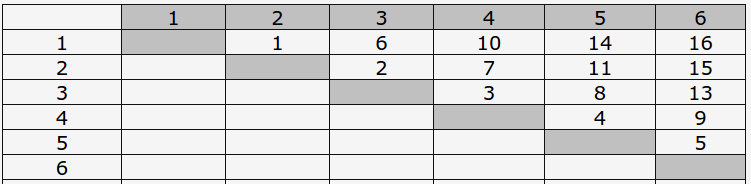
\includegraphics[width=8cm]{03/diagon}
\end{center}
Złożoność obliczeniowa wynika z:
\begin{itemize}
	\item dla każdej diagonali d ($n - 1$ różnych diagonali)
	\item dla każdej pozycji w~diagonali ($n - d$ pozycji)
	\item znajdź najlepszy podział ($j - i$ różnych wartości k, $ m(i,j) = \min\{m(i,k) + m(k+1, j) + p_{i-1} \cdot p_k \cdot p_j : i \le k < j\}$)
\end{itemize}

\subsection{Podsumowanie}
\begin{itemize}
	\item Liczba Catanala - \textbf{wykładnicza, $O(4^nn^\frac{-3}{2})$}
	\item Rekurencja (wielkość drzewa wywołań) - \textbf{wykładnicza, $O(2^{n-1})$}
	\item Programowanie dynamiczne - \textbf{potęgowa, $O(n^3)$ i $O(n^2)$}
	\item Szczegóły pod linkiem \href{http://edu.pjwstk.edu.pl/wyklady/asd/scb/asd14/main14_p2.html}{tutaj}
\end{itemize}




\section{Drzewie binarnym przeszukiwanie zgodnie z porządkiem inorder ma postać}

\vspace{0.4cm}
\noindent \textbf{Proponowana odpowiedź:} Zbadaj według kolejności: wierzchołek, lewe poddrzewo, prawe poddrzewo. \\

\noindent \textbf{Odpowiedź:} Zbadaj według kolejności: lewe poddrzewo, wierzchołek, prawe poddrzewo. \\

\noindent \textbf{Wyjaśnienie:}
\begin{figure}[h]	
	\centering	
	\subcaptionbox{Pre-order}
    {
		\begin{tikzpicture}[->,>=stealth',level/.style={sibling distance = 2cm/#1,level distance = 1.5cm},scale=0.6, transform shape]
		\node [treenode] {$1$}
		child { node [treenode] {$2$} }
		child { node [treenode] {$3$ } };
		\end{tikzpicture}
	}\qquad\qquad
    \subcaptionbox{In-order}
	{
		\begin{tikzpicture}[->,>=stealth',level/.style={sibling distance = 2cm/#1,level distance = 1.5cm},scale=0.6, transform shape]
		\node [treenode] {$2$}
		child { node [treenode] {$1$} }
		child { node [treenode] {$3$ } };
		\end{tikzpicture}
	} \qquad\qquad
	\subcaptionbox{Post-order}
	{
		\begin{tikzpicture}[->,>=stealth',level/.style={sibling distance = 2cm/#1,level distance = 1.5cm},scale=0.6, transform shape]
		\node [treenode] {$3$}
		child { node [treenode] {$1$} }
		child { node [treenode] {$2$ } };
		\end{tikzpicture}
	}
\end{figure} \\



\section{Złożoności}

\textbf{Zadanie o~rozmiarze $n$, realizowane pewnym algorytmem o~złożoności $f(n)$, zostało sprowadzone do~dwóch podzadań o~rozmiarze $\frac{n}{2}$ kazde oraz do~$n$~działań o~stałym czasie wykonania, zapewniających rozbicie i~scalenie zadania. Złożoność $f(n)$ wynosi:}\\
\textit{Przykładowa odp.) $f(n) = O(n\log{n})$}

\vspace{0.4cm}
\subsection{Wprowadzenie -- rodzaje złożoności}
\begin{description}
	\item[złożoność praktyczna] -- dla~podanego rozmiaru danych wyznacza dokładną liczbę elementarnych kroków potrzebnych do~wykonania danego algorytmu (oznaczenie \textbf{$T$})
	\item[złożoność teoretyczna] -- (klasa algorytmu) określa, jak silnie zależą od~siebie: rozmiar danych i~czas wykonania algorytmu - przy założeniu, że ten pierwszy wzrasta nieograniczenie (oznaczenie \textbf{$\Theta$})
	\item[notacja asymptotyczna] -- jeżeli $g(n)$ należy zarówno do $\Omega(f(n))$, jak i~do~$O(f(n))$, to~z~pewnością należy także do~$\Theta(f(n))$ 
	\begin{description}
		\item[dokładna] $ \Theta (f(n)) = \{ g(n): \exists_{c_1, c_2,n_0 > 0} \forall_{n \ge n_0} 0 \le c_1 f(n) \le g(n) \le c_2 f(n)  \} $
		\item[górne] $ O(f(n)) = \{ g(n): \exists_{c,n_0 > 0} \forall_{n \ge n_0} 0 \le g(n) \le c f(n)  \} $
		\item[dolne]$ \Omega (f(n)) = \{ g(n): \exists_{c,n_0 > 0} \forall_{n \ge n_0} 0 \le  c f(n) \le g(n) \} $
	\end{description}
\end{description}
\subsection{Rozwiązanie}
Korzystamy z~twierdzenia o~rekurencji uniwersalnej:
Niech $a \ge 1$ i $b > 1$ będą stałymi, $f(n)$ dowolną funkcją, zaś $T(n)$ zdefiniowane dla~nieujemnych liczb całkowitych poprzez rekurencję:
$$T(n) = aT(\frac{n}{b}) + f(n)$$
Wówczas $T(n)$ możemy asymptotycznie oszacować w~następujący sposób:
\begin{enumerate}
	\item Jeśli $f(n) = O(n^{\log_b {(a -\epsilon)}})$ dla pewnej stałej $\epsilon > 0$, to $T(n) = \Theta(n^{\log_b a})$
	\item Jeśli $f(n) = \Theta(n^{\log_b {a}})$, to $T(n) = \Theta(n^{\log_b a} \log n)$
	\item Jeśli $f(n) = \Omega(n^{\log_b {(a + \epsilon)}})$ dla pewnej stałej $\epsilon > 0$, to $T(n) = \Theta(f(n))$
\end{enumerate}

Oznaczenia mogą być trochę mylące. Niech $f$ z~treście pytania będzie oznaczone $T$. Wtedy $T(n) = 2T(\frac{n}{2}) + n$. Funkcja $f$ z~twierdzenia to~$n$, $a = 2$, $b = 2$, $\log_2 2 = 1 $, więc spełniony jest podpunkt 2. Odpowiedź to~\textbf{$\Theta(n\log n)$} (a~więc także $O(n\log n)$ i~$\Omega (n\log n)$).





\section{Dany jest graf skierowany G = (V,E), gdzie V =\{1,2,3,4,5,6\}, E = \{(1,2), (1,3), (2,4), (2,5), (4,5), (5,1), (3,5), (3,6)\}. Jeśli graf G przeszukujemy w głąb poczynając od wierzchołka 1 to}

\vspace{0.4cm}
\noindent \textbf{Proponowana odpowiedź:} Krawędź (2,5) może być krawędzią drzewową (w zależności od realizacji algorytmu) \\

\noindent \textbf{Odpowiedź:}  
\begin{itemize}
	\item Możliwa kolejność odwiedzonych wierzchołków: $1, 2, 4, 5, 3, 6$
	\item Krawędzie drzewowe: $(1, 2), (2, 4), (4, 5), (1, 3), (3, 6)$.
	\item Krawędzie wprzód: $(2, 5), (3, 5)$
	\item Krawędzie powrotne: $(5, 1)$
	\item Krawędzie $(2,5), (3, 5)$ może być drzewowe, w zależności od realizacji algorytmu 
	\item Krawędź $(4, 5)$ może być wprzód, w zależności od realizacji algorytmu 
\end{itemize}

\noindent \textbf{Wyjaśnienie:}
Zbiór wszystkich drzew przeszukiwania w głąb - które zostały utworzone podczas przechodzenia po grafie - nazywamy lasem przeszukiwania w głąb.
Przechodząc pod grafie możemy dokonać klasyfikacji krawędzi na:
\begin{itemize}
	\item krawędzie drzewowe - są to krawędzie których zbadanie powoduje odkrycie nowego wierzchołka
	\item krawędzie powrotne - są to krawędzie łączące wierzchołek z przodkiem
	\item krawędzie w przód - są to krawędzie niedrzewowe, łączące wierzchołek z potomkiem
	\item krawędzie poprzeczne - wszystkie inne krawędzie
\end{itemize}  


\section{Zgadywanka}
\textbf{Które stwierdzenia sposród poniższych są prawdziwe (haha.)}\\
\textit{przykładowa odp.) Algorytm Dijkstry ma własność optymalnej podstruktury,}

\vspace{0.4cm}

Przykładowa odpowiedź jest prawdziwa, bo ``The subpath of~any~shortest path is~itself a~shortest path'', a~problem z~optymalną podstrukturą to~taki, którego optymalne rozwiązanie może być~efektywnie skonstruowane z~optymalnych rozwiązań podproblemów. Zwykle własność optymalnej podstruktury oznacza, że problem może być rozwiązany algorytmem zachłannym lub dynamicznym.




\section{Dana jest procedura xxx. Przyjmij konwencję, że np. zapis AAABCC oznacza trzykrotne wykonanie instrukcji A, po czym następuje wykonanie instrukcji B a następnie dwukrotnie instrukcji C. Następujące sekwencje instrukcji mogą być wynikami wywołania powyższej procedury}
\begin{lstlisting}
Proc(n) {
	if (warunek(x)) then {
		A(x);
		Proc(f(n));
		B(x);
	} else
		C(x);
}
\end{lstlisting}

\vspace{0.4cm}
\noindent \textbf{Proponowana odpowiedź:} AAACCCBBB \\ 

\noindent \textbf{Odpowiedź:} $A^xCB^x, x \ge 0$ \\

\noindent \textbf{Wyjaśnienie:}
Funkcja Proc jest rekurencyjnie wywoływana pomiędzy wywołaniem A i B. W przypadku kiedy warunek jest spełniony, Proc rozpoczyna się od wywołania funkcji A, następnie rekurencyjnie wywołuje siebie, odkładając wywołanie funkcji B "na później". Będzie to następować tak długo jak warunek jest spełniony. W momencie kiedy warunek będzie niespełniony nastąpi wywołanie funkcji C oraz pozostałe wywołania funkcji B odłożone na stosie wywołań. \\

\section{BST}
\textbf{Graf $G = (V, E)$ jest drzewem BST, przy czym $V = \{15, 21, 23, 29, 31, 38, 40, 61, 96, 98\}$, $E = \{(21, 15),(21, 23),(29, 21),(29, 31),(38, 29),(38, 96),(96, 40),(96, 98),(40, 61)\}$.}\\
\textit{przykładowa odp.) W wyniku przeszukiwania postorder wierzchołki zostaną odwiedzone w następującej kolejności: 15, 23, 21, 29, 31, 61, 40, 98, 96, 38.}

\vspace{0.4cm}

Na~podstawie krawędzie łatwo można narysować taki graf

\begin{center}
	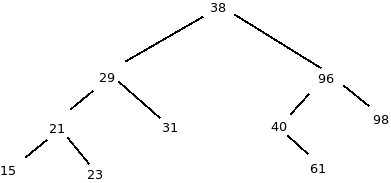
\includegraphics[width=8cm]{03/bst}
\end{center}

Mamy trzy możliwe rodzaje przejść Depth First:
\begin{itemize}
	\item preorder (vlr) 
	\begin{lstlisting}
	preorder(node)
	if node == null then return
	visit(node)
	preorder(node.left) 
	preorder(node.right)
	\end{lstlisting}
	- wynik:  38, 29, 21, 15, 23, 31, 96, 40, 61, 98
	\item inorder (lvr) 
	\begin{lstlisting}
	inorder(node)
	if node == null then return
	inorder(node.left)
	visit(node)
	inorder(node.right)
	\end{lstlisting}
	- wynik: 15, 21, 23, 29, 31, 38, 40, 61, 96, 98
	\item postorder (lrv)
	\begin{lstlisting}
	postorder(node)
	if node == null then return
	postorder(node.left)
	postorder(node.right)
	visit(node)
	\end{lstlisting}
	- wynik: 15, 23, 21, 31, 29, 61, 40, 98, 96, 38
\end{itemize}

Możliwe jest także przejście Breadth-First (odwiedzany jest każdy węzeł na~poziomie przed zejściem na~kolejny poziom). Wynik: 38, 29, 96, 21, 31, 40, 98, 15, 23, 61.\\
Przykładowa odpowiedź jest nieprawdziwa.


\section{Niech $p=(x_1, y_1)$, $q=(x_2, y_2)$, $r=(x_3, y_3)$ oraz $det(p, q, r)$, oznacza wyznacznik macierzy}
\noindent $x_1 \quad y_1 \quad 1$ \\
$x_2 \quad y_2 \quad 1$ \\
$x_3 \quad y_3 \quad 1$


\vspace{0.4cm}
\noindent \textbf{Proponowana odpowiedź:} Jeśli $det(p, q, r) = 0$ to punkt $r$ leży na prostej wyznaczonej przez punkty p i q \\ 

\noindent \textbf{Odpowiedź:}
\begin{itemize}
	\item Jeśli $det(p, q, r) > 0$ to punkt $r$ leży po lewej stronie wektora p $\rightarrow$ q
	\item Jeśli $det(p, q, r) = 0$ to punkt $r$ leży na prostej wyznaczonej przez punkty p i q
	\item Jeśli $det(p, q, r) < 0$ to punkt $r$ leży po prawej stronie wektora p $\rightarrow$ q
	\item Jeśli $sgn(det(p, q, p_1)) = sgn(det(p,q, p_2))$, punkty $p_1$ i $p_2$ leżą po tej samej stronie prostej $p - q$
\end{itemize}

\noindent \textbf{Wyjaśnienie:}
Algorytmy geometryczne. Wzięte z wykładów prof. Bieleckiego.


\section{Problem przynależności punktu do wielokąta}

\textbf{Danych jest n~punktów wyznaczających wielobok o~n~bokach.}\\
\textit{przykładowa odp.) Istnieje algorytm o~złozoności $O(\log n)$ sprawdzający, czy~zadany punkt nalezy do~wnętrza wieloboku.}

\vspace{0.4cm}

\subsection{Problem}
No~dobra, ogarnijmy o~co~chodzi w~zagadnieniu. Będzie fajnie.

Dla danego punktu p~sprawdź, czy~p~znajduje się~wewnątrz, czy~na~zewnątrz n-kąta reprezentowanego przez ciąg kolejnych krawędzi.
\subsection{Zliczanie przecięć krawędzi}

\begin{lstlisting}
poprowadz z p pionowa polprosta l;
k:=0; 
wybierz bok wielokata f;
repeat
if  l przecina f
then k:=k+1;
f:=kolejny bok wielokata;
until wszystkie boki wielokata zostaly zbadane; 
if  k parzyste then p jest na zewnatrz
else p jest wewnatrz;
\end{lstlisting}

Widzimy, że~złożoność algorytmu to~$O(n)$. Algorytm nie~bierze pod~uwagę przypadków szczególnych (półprosta zawiera wierzchołek/krawędź) -- ich~uwzględnienie nie~zmienia złożoności obliczeniowej.

Ok, dalej: lokalizacja punktu względem wielokąta wypukłego. Problem prostszy.

Definicja: Górnym (dolnym) łańcuchem wielokąta wypukłego nazywamy ciąg jego krawędzi między skrajnie lewym a~skrajnie prawym wierzchołkiem wielokąta odwiedzanych zgodnie z~ruchem wskazówek zegara (przeciwnie do~ruchu wskazówek zegara).
\begin{center}
	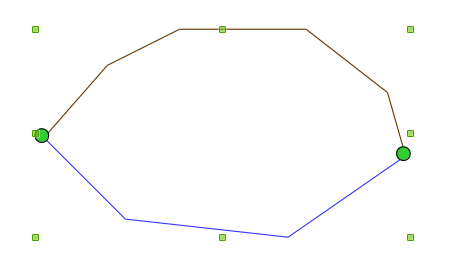
\includegraphics[width=4cm]{03/lancuch}
\end{center}

Półprosta poprowadzona z~danego punktu przecina każdy z~łańcuchów wielokąta wypukłego w~co~najwyżej jednym punkcie (jeśli przetnie dwa razy, jest poza; jeśli raz, jest w~środku).

Wyszukiwanie przecięcia:
krawędzie łuku mamy w~tablicy, zaczynamy od~środkowego elementu i~w~zależności, czy~półprota jest po~prawej czy~po~lewej idziemy w~odpowiednią stronę. Jest to~przeszukiwanie drzewa, a~więc $O(\log n)$.

Dla uogólnienia problemu do~przestrzeni \textbf{trójwymiarowej} istnieje analogiczny algorytm o~złożoności $O(n)$.

\subsection{Zliczanie zakrętów}
Winding Number Algorithm -- zliczamy ile razy krawędzie ``skręcają'' w~lewo (+1) i~ile w~prawo (-1), jeśli wyjdzie 0 mamy pełny obrót (jesteśmy w~środku).

Jeśli jesteśmy po~lewej stronie krawędzi skierowanej w~lewo, zakręt w~lewo.\\
Jeśli jesteśmy po~prawej stronie krawędzi skierowanej w~prawo (patrząc zgodnie ze~strzałką), zakręt w~prawo.
\begin{center}
	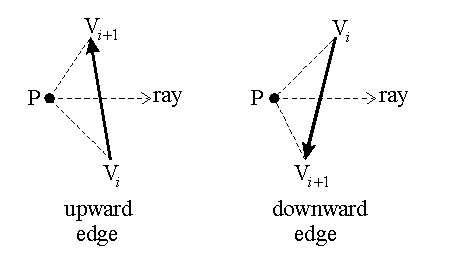
\includegraphics[width=6cm]{03/uede}
\end{center}

\begin{lstlisting}
wn_PnPoly( Point P, Point V[], int n )
{
int    wn = 0;    // the  winding number counter

// loop through all edges of the polygon
for (each edge E[i]:V[i]V[i+1] of the polygon) {
if (E[i] crosses upward ala Rule #1)  {
if (P is  strictly left of E[i])    // Rule #4
++wn;   // a valid up intersect right of P.x
}
else
if (E[i] crosses downward ala Rule  #2) {
if (P is  strictly right of E[i])   // Rule #4
--wn;   // a valid down intersect right of P.x
}
}
return wn;    // =0 <=> P is outside the polygon

}
\end{lstlisting}

Złożoność $O(n)$.
\subsection{Podsumowanie}
\begin{itemize}
	\item dla wielokąta w~2D: $O(n)$
	\item dla wielokąta wypukłego w~2D: $O(\log n)$
	\item dla wielokąta w~3D: $O(n)$
	\item dla wielokąta w~2D istnieje jeszcze algorytm ``Winding Number'' (na~polski indeks punktu względem krzywej) o~złożoności $O(n)$.
\end{itemize}




\section{Graf dynamiczny, którego maksymalnej liczby wierzchołków i krawędzi w trakcie wykonywania algorytmu nie potrafimy z góry oszacować powinien być reprezentowany jako}


\vspace{0.4cm}
\noindent \textbf{Proponowana odpowiedź:} Lista list \\ 

\noindent \textbf{Odpowiedź:} Lista sąsiedztwa zaimplementowana jako lista list. \\

\noindent \textbf{Wyjaśnienie:}
Lista sąsiedztwa jest listą list. Każdy element głównej listy odpowiada jednemu wierzchołkowi $u$ opisywanego grafu. W liście przechowywane są wskaźnili na listy zawierające wierzchołki $v_x$ sąsiednie do $u$. Operacje w większości wykonują się wolniej niż w przypadku macierzy sąsiedztwa. Zaletą jest duża elastyczność w przypadku zmiany ilości wierzchołków oraz mniejsza złożoność pamięciowa, liniowa względem krawędzi.



\section{Problem komiwojażera}

\textbf{Dla problemu komiwojażera algorytm pozwalający wyznaczyć rozwiązanie optymalne:}\\
\textit{przykładowa odp.) istnieje i ma złozoność wykładniczą}

\vspace{0.4cm}


\subsection{Problem}
Dany pełny graf n-wierzchołkowy z~nieujemnymi wagami na~krawędziach. Znaleźć cykl Hamiltona (cykl, w~którym każdy wierzchołek odwiedzony jest dokładnie raz) o~najmniejszej wadze (tzn. sumie wag krawędzi).

\noindent Problem należy do~klasy NP-hard (NP-trudnych).\\
Problem \textbf{decyzyjny} komiwojażera należy do~klasy NP-complete (NP-zupełnych).\\
Problem \textbf{metryczny} komiwojażera należy do~klasy NP-complete (NP-zupełnych). (spełniona jest nierówność trójkąta dla każdej trójki wierzchołków).\\

\subsection{Algortymy}
\begin{itemize}
	\item istnieje algorytm o~złożoności wykładniczej względem liczby wierzchołków wyznaczający rozwiązanie optymalne
	\item dla metrycznego problemu komiwojażera istnieje \textbf{algorytm 2-aproksymacyjny} o~złożoności \textbf{wielomianowej} (znalezione rozwiązanie jest lepsze niż drukrotność optymalnego)
	\item dla metrycznego problemu komiwojażera istnieje \textbf{algorytm $\frac{3}{2}$-aproksymacyjny} o~złożoności \textbf{wielomianowej} - jak na~razie najlepszy stopień przybliżenia rozwiązania
	\item dla klasycznego algorytmu komiwojażera nie istnieje żaden algorytm aproksymacyjny (o~ile P != NP, brak dowodu)
\end{itemize}

Algorytm 2-apryksymacyjny: (chyba tutaj niepotrzebny, dlatego nie rozwijany zanadto)
\begin{enumerate}
	\item Znajdź minimalne drzewo spinające T (algorytm Prima, minimalne drzewo rozpinające -- algorytm oblicza podzbiór E' zbioru krawędzi E, dla którego graf nadal pozostaje spójny, ale suma kosztów wszystkich krawędzi zbioru E' jest najmniejsza możliwa)//
	w~skrócie wywalamy wszystkie krawędzie tak, żeby można było dostać się~z~każdego wierzchołka do~innego wierzchołka, i~żeby suma wag krawędzi była najmniejsza; złożoność algorytmu zależy od~zastosowanej struktury danych.
	\item Dodaj krawędzie tak aby stopień każdego wierzchołka był parzysty (stopień = liczba wychodzących krawędzi)
	\item Otrzymany graf  X jest eulerowski (da~się w~nim skonstruować cykl Eulera, czyli cykl, który przechodzi przez każdą jego krawędź dokładnie raz i~wraca do punktu wyjściowego)
	\item Przekształć cykl Eulera w cykl Hamiltona
\end{enumerate}


\section{Głębokość rekurencji dla ciągu Fibonacciego zaimplementowanego rekurencyjnie zgodnie z arytmetyczną definicją rekurenycjną wynosi}

\vspace{0.4cm}
\noindent \textbf{Proponowana odpowiedź:} $O(n^4)$ \\ 

\noindent \textbf{Odpowiedź:} $O(2^n)$ \\

\noindent \textbf{Wyjaśnienie:}
$T(n) = T(n-1) + T(n-2) + c \leq 2T(n-1) + c = 2(2T(n-2) + c) + c = 2^2T(n-2) + 2c + 2^0c =...= 2^nT(0) + 2^{n-1}c + ... + 2c + 2^0c = c(2^n-1)$ \\


\section{Kursorowa implementacja listy}
\textbf{Kursorowa implementacja listy jest strukturą}\\
\textit{przykładowa odp.) rekordową}

\vspace{0.4cm}


\subsection{Kursorowa implementacja listy}
W~językach nie posiadających referencji ani wskaźników nie~istnieje możliwość klasycznej implementacji listy. Z~tego powodu stosuje się~tablicę \textbf{rekordów}. Każdy rekord przechowuje wartość elementu oraz indeks wskazujący, na~którym miejscu w~tablicy znajduje się~kolejny element (w~przypadku listy podwójnie wiązanej, zarówno następny jak i~poprzedni).

\begin{lstlisting}
record Entry {
integer next; // index of next entry in array
integer prev; // previous entry (if double-linked)
string name;
real balance;
}
\end{lstlisting}
Dodatkowo konieczne jest przechowywanie osobno indeksu pierwszego elementu listy.

``W~celu sprawniejszego znajdowania miejsca wolnego w~tablicy, można wszystkie wolne miejsca powiązać w~tzw. \textbf{listę pamięci wolnej}, w~której pierwszy element jest przechowywany przez  globalną zmienną o~nazwie np.~firstfree'' A. Bielecki 

\subsection{Odpowiedź}
Tak, jest strukturą \textbf{rekordową}. Jest też \textbf{tablicową} (tak?)

\section{Problem chińskiego listonosza polega na}
\noindent \textbf{Proponowana odpowiedź:} Znalezieniu najkrótszej drogi zamkniętej zawierającej wszystkie wierzchołki grafu. \\

\noindent \textbf{Odpowiedź}:  Znalezieniu najkrótszej drogi zamkniętej zawierającej wszystkie \textbf{krawędzie} grafu. \\

\noindent \textbf{Wyjaśnienie}:
Rozważmy graf, którego krawędzie odpowiadają ulicom w rejonie, obsługiowanym przez listonosza. Wierzchołki to po prostu skrzyżowania ulic. Krawędziom nadajemy wagi, które oznaczają odległości między dwoma skrzyżowaniami. Znalezienie możliwie najkrótszej drogi, którą musi przejść listonosz sprowadza sie do znalezienia w tym grafie drogio minimalnej sumie wag krawędzi, która przechodzi przez każdą krawędź co najmniej raz. Jeśli dany graf posiada cykl Eulera, to istnieje taka droga, która zaczyna i konczy sie w tym samym punkcie i wymaga przejścia po każdej ulicy dokładnie raz. Problem ma zawsze rozwiązanie jeżeli graf jest spójny. 
\chapter{Podstawy grafiki komputerowej}
\PartialToc
%\startcontents[chapters]
%\printcontents[chapters]{}{1}{\section*{\contentsname}}
\section{Na czym polega rendering obiektu w grafice?}
Na przekształceniu struktury 3D w obraz rastowy 2D. \\
Proces ten jest niezwykle skomplikowany i uwzględnia szereg różnorodnych zmiennych, jak na przykład punkt widzenia, system rzutowania, położenie obiektów, oświetlenie. Podczas renderingu wyliczane są m.in. odbicia, cienie, załamania światła, mgła, atmosfera, efekty wolumetryczne. Jest to bardzo czasochłonna operacja nie wymagająca, poza przygotowaniem, żadnej ingerencji ze strony człowieka.

\section{Proszę podac która wersja etapów w tzw. „graphics pipeline” jest poprawna.}
Display, Modeling transformation, Viewing transformation, Preventex lighting, Projection, Clipping, Scan conversion or rasterization, Texturing

\section{Proszę podac jakie są podstawowe (dziś) typy grafiki komputerowej?}
Wektorowa, Rastrowa. Inny podział 2D, 3D.

\section{Czym rózni się OpenGL od Direct3D? }
OpenGL jest multi-platformowe i jest typu open source. Direct3D jest wydajniejszy.

\section{Jakie są 3 podstawowe transformacje w grafice komputerowej i jaki aparat matematyczny jest używany do liczenia transformacji obiektów na scenie?}
Translacja, Rotacja, Skalowanie. Liczone przy użyciu macierzy.

\section{Co to jest Ray Tracing?}
Jest to metoda przemieszczania promienia skanującego.\\
Umożliwia tworzenie fotorealistycznych obrazów ze scen trójwymiarowych. Opiera się na analizowaniu tylko tych promieni światła, które trafiają bezpośrednio do obserwatora. W rekursywnym śledzeniu promieni bada się dodatkowo promienie odbite, zwierciadlane oraz załamane.

\section{Jakim skrótem oznacza się powszechnie procesor graficzny?}
GPU

\section{Co to jest fraktal?}
Jest to obiekt samopodobny. \\ Obiekt matematyczny posiadający własność samopodobieństwa. Grafika fraktalna wykorzystywana jest zwykle do generacji losowych krajobrazów oraz map geograficznych. Charakterystyczną cechą tego rodzaju grafiki jest możliwość nieskończonego powiększania dowolnego elementu obrazu. np. płatki śniegu, system naczyń krwionośnych, systemy wodne rzek, błyskawica.

\section{Co oznacza NURBS?}
Non Uniform Rational B-Splines. Sposób opisu krzywej lub powierzchni za pomocą formuły matematycznej. Jest lżejszym i bezstratnym opisem tych brył. Konkurencją dla opisu za pomocą trójkątów. Coś jak grafika wektorowa dla rastowej.

\section{Co to jest Z-buforowanie?}
Jest to sprzetowy algorytm liczenia które fragmenty sceny są widoczne.
Polega na pamiętaniu informacji o odległości od kamery (głębokości) każdego piksela.

\chapter{Programowanie obiektowe}
\PartialToc
%\startcontents[chapters]
%\printcontents[chapters]{}{1}{\section*{\contentsname}}

% ~~~~~~~~~~~~~~~~~~~~~~~~~ 1
\answer
{Jakie są typ i wartość wyrażenia 2 + "2.68"?}
{Wyrażenie jest niezgodne ze składnią języka.}
{F}
{Będzie  to string o wartości "22.68"}
{String + int = String}

% ~~~~~~~~~~~~~~~~~~~~~~~~~ 2
\answer
{Aby sprawdzić, czy dwa obiekty typu String mają taką samą zawartość można:}
{Użyć operatora $==$}
{F}
{Użyć metody \textbf{equals} klasy String - s1.equals(s2).}
{Operator == porównuje w tym wypadku referencje do obiektów, a nie ich zawartość. Do tego służą w Javie metody equals. Teoretycznie operator == mógłby być użyty dla porównania Stringów, jeśli pochodziły by one ze wspólnej puli napisów (wcześnie wywołano na nich metodę intern())}

% ~~~~~~~~~~~~~~~~~~~~~~~~~ 3
\answer
{Który z poniższych fragmentów kodu sprawdza, czy obiekt wskazywany przez referencję xyz należy do klasy XYZ?}
{
	\begin{lstlisting}[language=java]^^J
if (xyz.dynamicCastTo(XYZ.class) != null)^^J
	\end{lstlisting}
}
{F}
{
\begin{lstlisting}[language=java]^^J
// Method #1^^J
xyz instanceof XYZ^^J
^^J
// Method #2^^J
XYZ.class.isInstance(xyz)^^J
^^J
// Method #3^^J
XYZ.class.isAssignableFrom(xyz.getClass())^^J
^^J
// Method #4^^J
try {
    XYZ c = (XYZ) xyz;^^J
    // No exception: xyz is of type XYZ or IT MIGHT BE NULL!^^J
} catch (ClassCastException e) {^^J
}^^J
// Method #5^^J
try {^^J
    XYZ c = XYZ.class.cast(xyz);^^J
    // No exception: xyz is of type XYZ or IT MIGHT BE NULL!^^J
} catch (ClassCastException e) {^^J
}	^^J
\end{lstlisting}
}
{Inne możliwości oraz szersze wyjaśnienie - \url{http://stackoverflow.com/questions/541749/how-to-determine-an-objects-class-in-java} }

% ~~~~~~~~~~~~~~~~~~~~~~~~~ 4

\section{Który z fragmentów kodu poprawnie wypisze elementy tablicy, zdeklarowanej jako:}
\begin{lstlisting}[language=java]
int tab[] = new int[] {3, 2, 1, 0};
\end{lstlisting}


\begin{lstlisting}[language=java]
for ( int i:tab )
	System.out.println(i +" ");
\end{lstlisting}

\textbf{PRAWDA}

\vspace{0.4cm}
\noindent
\textbf{Odpowiedź:}
Petla foreach (j.w.), for:
\begin{lstlisting}[language=java]
for ( int i = 0; i < tab.length; i++ )
	System.out.println(tab[i]+" ");
\end{lstlisting}
while:
\begin{lstlisting}[language=java]
int i = 0;
while ( i < tab.length )
	System.out.println(tab[i++] +" ");
\end{lstlisting}
i wiele innych możliwości.
\vspace{0.4cm}
\noindent

% ~~~~~~~~~~~~~~~~~~~~~~~~~ 5

\section{Przeanalizuj poniższy kod. Co zostanie wypisane?}
\begin{lstlisting}[language=java]
loop : for(int i = 0; i<3; i++){
  for(int j = 0; j<5; j++){
    System.out.print(i + j);
    if(j==1) break loop;
  }
}
\end{lstlisting}

\noindent
\textbf{Przykładowa odpowiedź:} 0011223
\textbf{FAŁSZ}

\vspace{0.4cm}
\noindent
\textbf{Odpowiedź:} 01

\vspace{0.4cm}
\noindent
\textbf{Wyjaśnienie:} Instrukcja break z etykieta przenosi nas do pierwszej linii poza blokiem oznaczonym ta etykieta.

% ~~~~~~~~~~~~~~~~~~~~~~~~~ 6
\answer
{Które zdanie opisujące własności klas jest prawdziwe?}
{Dla każdej klasy w języku Java możliwe jest zdefiniowanie klasy potomnej}
{F}
{\begin{itemize}
	\item Klasa może być zadeklarowana jako publiczna (public), wówczas jest dostępna z innych pakietów.
 	\item Klasy mogą być zadeklarowane jako abstrakcyjne (abstract), jeśli deklarują lub dziedziczą niezaimplementowane metody abstrakcyjne.
 	\item Klasy finalne (final) nie mogą mieć klas potomnych.
  	\item Wszystkie klasy poza klasa Object są klasami potomnymi jakiejś innej klasy. 
  	\item W ciele klasy mogą znajdować się:
    \begin{itemize}
 	 	\item deklaracje pól i metod składowych obiektów,
 	 	\item konstruktory,
 	 	\item deklaracje pól i metod statycznych,
 	 	\item deklaracje klas wewnętrznych
 	\end{itemize}
  	\item Elementom deklarowanym wewnątrz klasy można przypisywać standardowe modyfikatory określające prawa dostępu (public, protected, private).
  	\item Klasa może dziedziczyć tylko po jednej klasie bazowej (brak wielodziedziczenia).
  	\item Klasy mogą implementować jeden lub kilka interfejsów.
\end{itemize}}
{}

% ~~~~~~~~~~~~~~~~~~~~~~~~~ 7
\answer
{Które zdanie opisujące własności klas jest prawdziwe?}
{Klasa możne implementować wiele interfejsów}
{T}
{Powtórzone poprzednie pytanie}
{}

% ~~~~~~~~~~~~~~~~~~~~~~~~~ 8
\answer
{Które zdanie dotyczące trybów dostępu w języku Java jest prawdziwe?}
{Pola i metody prywatne nie są dziedziczone}
{F}
{
\begin{itemize}
\item[] \textbf{private} - element widoczny tylko w ramach instancji tej samej klasy
\item[] \textbf{domyślny - package} - element widoczny w ramach tego samego pakietu
\item[] \textbf{protected} - element widoczny jak powyżej, ale w dodatku dostępny także dla podklas danej klasy
\item[] \textbf{public} - element widoczny dla wszystkich klas
\end{itemize}
}
{}

% ~~~~~~~~~~~~~~~~~~~~~~~~~ 9
\answer
{Która kombinacja modyfikatorów metod jest dopuszczalna}
{static synchronized}
{T}
{Modyfikatory opcjonalne metod (kolejność dowolna, w jednym punkcie wykluczają się): 
   \begin {description}
	 \item [public / protected / private] modyfikatory dostępu
     \item [final / abstract] final blokuje możliwość rozszerzenia metody w klasach pochodnych, abstract sygnalizuje, że metoda nie ma ciała i należy ją rozszerzyć w klasie pochodnej
     \item [abstract / static] abstract poisane wyżej, static oznacza, że metoda istnieje nawet jeżeli nie istnieje instancja obiektu
     \item [strictfp / native] native sygnalizuje, że chcemy użyć języka innego niż java, a strictfp zapewnia, że operacje zmiennoprzecinkowe wykonane na różnych maszynach zwrócą dokładnie taki sam wynik
     \item [synchronized] powoduje, że metoda chroniona jest przez sekcje krytyczną
   \end {description}}
{}

% ~~~~~~~~~~~~~~~~~~~~~~~~~ 10
\answer
{Które ze stwierdzeń jest prawdziwe}
{Wszystkie tablice są klonowalne (realizuja interfejs Cloneable)}
{T}
{Pytanie zbyt ogólne do odpowiedzi.}
{}

% ~~~~~~~~~~~~~~~~~~~~~~~~~ 11
\answer
{W jaki sposób usuwane są obiekty w języku Java?}
{Nie są programowo usuwane, to środowisko wykonawcze podejmuje decyzje czy i kiedy je usunąć}
{T}
{Usuwaniem obiektów w Javie zarządza specjalny proces JVM - Garbage Collector. Jego uruchamianiem i przebiegiem zarządza maszyna wirtualna, użytkownik nie ma możliwości wymusić jego przejścia. Istnieje wprawdzie wywołanie System.gc(), jednak jest to tylko sugestia dla VM. Sam GC działa w dwóch fazach - Marking, gdy oznacza wszystkie obiekty, do których istnieją odwołania jako "żywe" oraz Sweeping, gdy zwalnia pamięć zajmowaną przez nieoznaczone obiekty.}
{}

% ~~~~~~~~~~~~~~~~~~~~~~~~~ 12
\answer
{Które z poniższych stwierdzeń odnoszących się do konstruktorów klas są prawdziwe}
{Aby wywołać konstruktor nadklasy, należy w pierwszej instrukcji konstruktora dodać wywołanie super([lista parametrów])}
{T}
{
\begin{itemize}
	\item Konstruktor jest nieodłączną częścią klasy (abstrakcyjna klasa również posiada swój konstruktor),
	\item Istnieje on nawet wtedy, kiedy go jawnie nie napiszemy (konstruktor domyślny),
	\item Nie jest możliwe stworzenie obiektu klasy bez udziału konstruktora,
	\item Konstruktor MUSI mieć taką samą nazwę, jak nazwa klasy,
	\item Konstruktor nie może zwracać żadnego typu (nawet void),
	\item Konstruktor domyślny jest zawsze bezparametrowy,
	\item Konstruktor domyślny można wywołać tylko wtedy, gdy klasa nie posiada żadnego, zaimplementowanego konstruktora,
	\item Konstruktor może być przeciążany,
	\item Podczas wywołania konstruktora danej klasy, wywoływane są również wszystkie konstruktory klas nadrzędnych,
	\item Konstruktor, o ile posiada parametry, może ustawiać pola wartościami, które dostał jako argumenty, jeżeli konstruktor nie ma żadnych parametrów, wszystkie wartości pól obiektu, będą zainicjalizowane domyślnymi wartościami.
	\item Konstruktor może być oznaczony dowolnym specyfikatorem dostępu, nawet private (wykorzystywane np. przy implementacji wzorca projektowego Singleton),
	\item Każdy konstruktor ma jako pierwsze wyrażenie albo odwołanie do przeciążonego konstruktora ( this() ), albo do konstruktora z klasy nadrzędnej ( super() ), pamiętać należy, że wyrażenia te mogą być dodane przez kompilator w trakcie kompilacji, jeżeli nie zostaną napisane (nie znaczy to jednak, że zawsze trzeba je jawnie wpisywać w ciało konstruktora),
	\item Konstruktor nie może mieć zaimplementowane (używać) jednocześnie słowa kluczowego super() i this(), 
	\item Konstruktor klasy bazowej (super()), może być wywoływany bez parametrów lub z nimi (zależnie od konstruktorów klasy bazowej),
	\item Nie można wywołać metody, lub odwołać się do pola instancji klasy, przed operatorem super(),
	\item Tylko zmienne lub metody statyczne mogą być użyte jako cześć wywołania super (np. super(ClassX.PoleStatyczne) ),
	\item Interfejsy nie posiadają konstruktorów,
	\item Konstruktor nie może być wywołany bezpośrednio (tak jak metoda), wywołanie takie może mieć miejsce tylko w innym konstruktorze,
	\item Konstruktory nie s dziedziczone.
\end{itemize}
}
{}

% ~~~~~~~~~~~~~~~~~~~~~~~~~ 13
\answer
{Które ze stwierdzeń odnoszących się do wyjątków w języku Java są prawdziwe?}
{Po wygenerowaniu wyjątku, który nie został przechwycony program kończy działanie}
{F}
{\begin{itemize}
 	\item Wyjątek Exception dziedziczy po klasie Throwable,
  	\item Klauzura „throws” nie oznacza, że zostanie wyrzucony, a jedynie, że istnieje taka możliwość,
  	\item Po pojawieniu się wyjątku przerywane jest normalne wykonanie metody, w której wyjątek został wyrzucony. System rozpoczyna poszukiwanie odpowiedniego fragmentu kodu, który jest odpowiedzialny za obsługę wyjątku (ang. Exception handler).
  	\item Kod obsługi wyjątku ma postać: catch(ExceptionType e){…}
  	\item Poszukiwanie rozpoczyna się od metody, w której wyjątek został wyrzucony. Jeżeli w bieżącej metodzie kod obsługujący wyjątek nie zostanie odnaleziony, wówczas przeglądana jest w górę zawartość stosu wywołania metod, aż do znalezienia odpowiedniego handlera wyjątku. Handler może zostać dopasowany do wyjątku, jeżeli typem wyrzuconego wyjątku jest wyspecyfikowania klasa ExceptionType lub klasa potomna;
	\begin{itemize}
  		\item Jeżeli handler zostanie odnaleziony, wówczas następuje przekazanie do niego sterowania z pominięciem dalszych instrukcji, które znajdują się w metodzie, gdzie nastąpiło wyrzucenie wyjątku. Mechanizm ten nazywany jest przechwytywaniem wyjątków.
  		\item Jeżeli na stosie wywołań funkcji brak jest odpowiedniego kodu obsługi wyjątków, maszyna wirtualna kończy działanie wątku, lub programu jeżeli jest jednowątkowy.
	\end{itemize}
    \item Generowane wyjątki są obiektami. Ich stan pozwala przekazać szczegółowe informacje o typie i miejscu wystąpienia błędów. W szczególności obiekt może przechowywać komunikat (String) oraz zawartość stosu wywołań funkcji dostępną zazwyczaj dzięki metodzie printStackTrace().
\end{itemize}}
{}

% ~~~~~~~~~~~~~~~~~~~~~~~~~ 14
\answer
{Które z poniższych stwierdzeń odnoszących się do typów generycznych w języku Java są prawdziwe?}
{Nie jest możliwe utworzenie tablic typów parametryzowanych}
{T}
{}
{}

% ~~~~~~~~~~~~~~~~~~~~~~~~~ 15
\answer
{Które z poniższych stwierdzeń odnoszące się do klas wewnętrznych i zagnieżdżonych w języku Java są prawdziwe}
{Obiekt klasy wewnętrznej ma swój stan niezależny od innych obiektów powiązanych z obiektem klasy zewnętrznej}
{T}
{}
{
Można zdefiniować klasę wewnątrz innej klasy. Wtedy klasę znajdująca się wewnątrz nazywamy klasa zagnieżdżona. Zasięg zagnieżdżonej klasy jest ściśle związany z zasięgiem klasy zewnętrznej. Jeśli klasa B zostanie zdefiniowana wewnątrz klasy A, wtedy B jest znana wewnątrz A, ale nie poza nią. Zagnieżdżona klasa ma dostęp do wszystkich składowych, także prywatnych, należących do klasy zewnętrznej. Klasa zewnętrzna nie ma dostępu do składowych klasy zagnieżdżonej.

Istnieją dwa rodzaje klas zagnieżdżonych: statyczne i niestatyczne. Statyczna klasa zagnieżdżona posiada na początku modyfikator static. Ponieważ jest klasa statyczna, dostęp do składowych klasy zewnętrznej musi się odbywać przez konkretna nazwę obiektu (nie można odwoływać się do zmiennych klasy zewnętrznej w sposób bezpośredni). Z powodu tego ograniczenia bardzo rzadko stosuje się statyczne klasy zagnieżdżone.
}

% ~~~~~~~~~~~~~~~~~~~~~~~~~ 16
\answer
{Które z poniższych stwierdzeń odnoszących się do interfejsów w języku Java są prawdziwe}
{Każda metoda zadeklarowana wewnątrz interfejsu jest publiczna}
{T}
{\begin{itemize}
	\item Interfejsy mogą deklarować wyłącznie metody abstrakcyjne. Domyślnie metody te są publiczne.
 	\item Interfejsy mogą definiować stałe (atrybuty typu static final)
 	\item Deklarując interfejs, wprowadzamy nowy typ danych – referencję do interfejsu (czyli po prostu możemy stosować nazwę interfejsu tak, jak nazwy klas). Referencje te mogą być użyte jako atrybuty klas, parametry metod oraz zmienne lokalne (np. Interfejs xyz = new KlasaImplementujacaInterfejs()).
 	\item Pomiędzy interfejsami może występować relacja dziedziczenia (słowo kluczowe extends).
	\item Dany interfejs może dziedziczyć po kilku interfejsach. W tym przypadku możliwe jest dziedziczenie wielokrotne.
 	\item W programie można zaimplementować wiele hierarchii interfejsów. 
 	\item Klasy mogą implementować wiele interfejsów należących do różnych hierarchii.
\end{itemize}}
{}

% ~~~~~~~~~~~~~~~~~~~~~~~~~ 17
\answer
{Które stwierdzenie odnoszące się do wątków w języku Java jest prawdziwe}
{Maszyna wirtualna Javy rozróżnia priorytety wątków. W momencie, kiedy watek o wyższym priorytecie będzie w stanie gotowości, wywłaszczy on watek o niższym priorytecie.}
{T}
{Watki działają zazwyczaj w jednym kontekście aplikacji w ramach danej VM. Współdzielą one miedzy sobą stertę VM i otwarte pliki, ale każdy posiada własny stos. 

Watki można tworzyć poprzez implementacje interfejsu Runnable lub rozszerzenie klasy Thread.

Watek kończy działanie po:
\begin{itemize}
 \item zakończeniu wykonywania metody run(),
 \item pojawieniu się wyjątku, który nie został obsłużony,
 \item wywołaniu metody stop() – aktualnie jest to odradzane, a sama metoda ma status deprecated
 \end{itemize}
Aplikacja kończy działanie, gdy:
 \begin{itemize}
 \item Wszystkie watki zakończa swoja prace (deamony nie są brane pod uwagę),
 \item Pojawi się krytyczny wyjątek klasy Error
\end{itemize}
 }
{}

% ~~~~~~~~~~~~~~~~~~~~~~~~~ 18
\answer
{Które stwierdzenie odnoszące się do wątków w języku Java jest prawdziwe}
{ Zaleca się zakończenie wątku poprzez wyjście z metody run()}
{T}
{Powtórzone poprzednie pytanie.}
{}

% ~~~~~~~~~~~~~~~~~~~~~~~~~ 19
\answer
{Które stwierdzenia odnoszące się do monitorów w języku Java są prawdziwe}
{Watek będący właścicielem monitora może wywoływać inne metody synchroniczne. }
{T}
{Java pozwala synchronizować watki pracujące ze zmiennymi warunkowymi dzięki użyciu monitorów. Monitory związane są ze specyficznymi danymi (nazywanymi zmiennymi warunkowymi) i działają jako blokada zakładana na tych danych. Gdy watek zajmie monitor dla jakiejś danej, inne watki do czasu zwolnienia monitora zostają zablokowane i nie mogą odczytywać lub modyfikować danych.

Segment kodu w programie, w którym następuje dostęp do tej samej danej z różnych wątków nazywany jest sekcja krytyczna (ang. critical section). W Javie sekcje krytyczna oznaczmy przy użyciu słowa kluczowego synchronized.

W Javie każdy obiekt, który ma metody synchroniczne posiada swój monitor. W momencie gdy sterowanie znajdzie się w metodzie synchronicznej, wątek, który wywołał te metodę zajmuje monitor obiektu, którego metodę wywołano. Inne watki nie mogą wołać metod synchronicznych tego obiektu do czasu zwolnienia monitora. Monitory w Javie są wielodostępne (ang. reentrant). Oznacza to, że watek, który zajął monitor jakiegoś obiektu może wołać inne metody synchroniczne obiektu.

Operacje zajmowania i zwalniania monitora są wykonywane automatycznie przez środowisko wykonawcze Javy, co zapewnia integralność danych i chroni przed wystąpieniem sytuacji wyjątkowych spowodowanych operacjami na monitorach.}
{}

% ~~~~~~~~~~~~~~~~~~~~~~~~~ 20
\answer
{Które z poniższych stwierdzeń odnoszących się do rozwiązań stosowanych w bibliotece AWT jest prawdziwe?}
{Za rozmieszczenie komponentów odpowiada przypisany do kontenera obiekt klasy LayoutManager}
{T}
{Jeżeli do kontenera nie jest przypisany LayoutManager to komponenty zostaną ustawione przez domyślny LayoutManager}
{\url{http://www.tutorialspoint.com/awt/awt_layouts.htm}}

% ~~~~~~~~~~~~~~~~~~~~~~~~~ 21
\answer
{Które z poniższych stwierdzeń odnoszących się do obsługi zdarzeń w bibliotece AWT są prawdziwe}
{ Adapter to klasa zapewniająca puste implementacje metod interfejsu typu Listener}
{T}
{Do obsługi zdarzeń w AWT wykorzystywany jest wzorzec Listenera. Aby jakaś klasa mogła być zarejestrowana jako słuchacz elementu AWT musi implementować interfejs ActionListener, posiadający metodę actionPerformed(ActionEvent arg). Metoda ta jest wywoływana, gdy zostanie wygenerowane zdarzenie na obiekcie powiązanym z danym słuchaczem. Przekazywany jest wtedy jako argument obiekt klasy ActionEvent, zawierający informację m.in. o źródle zdarzenia, które można wykorzystać do podjęcia odpowiednich akcji.}
{Więcej o obsłudze zdarzeń w bibliotece AWT \url{http://www.cafeaulait.org/course/week7/19.html}}

% ~~~~~~~~~~~~~~~~~~~~~~~~~ 22
\answer
{Które z poniższych stwierdzeń odnoszących się do biblioteki Swing są prawdziwe}
{Ciężkimi komponentami w Swing są kontenery górnego poziomu: JFrame, JDialog i JApplet.}
{T}
{\begin{itemize}
\item Swing stanowi kolejna generacje biblioteki graficznej dla platformy Java. 
\begin{itemize}
\item Zapewnia bogaty zbiór komponentów graficznych (JLabel, JButton, JCheckBox, JComboBox, JTree, JTextField, JTextArea, itd.)
\item Został wyposażony w możliwość programowego zmieniania wyglądu aplikacji PLAF - Pluggable Look And Feel
\item Możliwości graficzne zostały rozszerzone o Java 2D API
\item Wsparcie dla internacjonalizacji
\end{itemize}
\item Swing przejął z AWT podstawowe zasady rozmieszczania komponentów z wykorzystaniem menadżerów układu oraz model obsługi zdarzeń. Podstawowa różnica pomiędzy komponentami Swing i AWT jest sposób implementacji komponentów
\item Projektując Swing przyjęto, że większość komponentów zostanie całkowicie napisanych języku Java i nie będą powiązane z odpowiednikami (peer) docelowej platformy. Są to właśnie lekkie komponenty (lightweight components). Jedynymi ciężkimi komponentami są kontenery górnego poziomu: JFrame, JDialog i JApplet.
\item Lekkie komponenty są potomkami klasy JComponent (dziedziczącej po java.awt.Container). Za ich wygląd i zachowanie odpowiada kod w całości napisany w języku Java. Dziki temu niezależnie od platformy reagują na zdarzenia w analogiczny sposób, zużywają mniej zasobów, działają szybciej, ponieważ wszelkie operacje odbywają się bez przekierowania do funkcji systemowych.
\end{itemize}
}
{}

% ~~~~~~~~~~~~~~~~~~~~~~~~~ 23
\answer
{Modelem dla komponentu Swing jest}
{Klasa elementu składowego (np. elementu listy), której obiekty przechowywane są w komponencie}
{T}
{
\begin{itemize}
\item Inspiracja dla architektury komponentów Swing był wzorzec MVC (model widok kontroler).
\item W architekturze komponentów Swing widok i kontroler zostały sprzężone w jeden obiekt nazywany UI Delegate, który skupia w sobie typowe zadania kontrolera i widoku oraz oddelegowuje cześć zadań widoku do obiektów specyficznych dla danej architektury PLAF dostarczanych przez klasę UIManager. Klasa bazowa dla różnych klas UI Delegate jest klasa ComponetUI
\begin{itemize}
\item Model przechowuje dane (ale też pełni cześć funkcji kontrolera, na przykład wysyła powiadomienia o zmianie w danych)
\item UI Delegate jest odpowiedzialny za pobieranie danych z Modelu i ich wizualizacje
\item Komponent koordynuje działanie Modelu i UI Delegate, a także stanowi interfejs do funkcjonalności biblioteki AWT
\end{itemize}
\end{itemize}
}
{}

% ~~~~~~~~~~~~~~~~~~~~~~~~~ 24
\answer
{W terminologii Swing Renderer to}
{ Pojedynczy obiekt, który jest odpowiednio konfigurowany, aby wyświetlić zawartość elementu umieszczonego w kontenerze}
{T}
{Jest to klasa używana przez złożone komponenty (lista, lista rozwijana, drzewo, tabela) do wizualizacji danych składowych.}
{}

\chapter{Architektury komputerów}
\PartialToc
%\startcontents[chapters]
%\printcontents[chapters]{}{1}{\section*{\contentsname}}

\newtheorem{pyt}{Pytanie}
\newtheorem{odp}{Odpowiedź}

\newenvironment{opracowanie}[1][1]{
	\newcounter{nr_pytania}
	\setcounter{nr_pytania}{#1}
}{}
\newcommand{\pytanie}[1]
{
\section{\arabic{nr_pytania}. IT1A\_W08,IT1A\_U8}
\stepcounter{nr_pytania}
\pyt \textbf{#1}
\par
}

\section{Wprowadzenie}

Przykładowe odpowiedzi nie kleją się z pytaniami, stąd właściwa odpowiedź rzadko będzie się odnosić do niej.
Pytania są dosyć lakoniczne i nierzadko pokrywają jeden czy dwa wykłady tego przedmiotu, dlatego odpowiedzi będą raczej w formie skrótu tematu, a w wyjaśnieniach będę starał się opisać sedno absurdu przykładowej odpowiedzi.
Będę starał się utrzymać konwencji w której pierwszy akapit jest najistotniejszy w danym pytaniu, a pozostałe, to pobieżne rozwinięte tematu, które warto raz przeczytać.

\section{FPGA}

W kilku pytaniach jest wspomniane o układach FPGA, lecz mało pytań jest bezpośrednio z tym układem związanych, dlatego pokrótce przypomnę, czym to jest.

FPGA - Field-Programmable Gate Array (Programowalna Macierz Bramek) jest to układ składający się z wielu \emph{bloków logicznych} i \emph{rejestrów} połączonych między sobą z użyciem \emph{macierzy połączeń}. Po więcej szczegółów, jak to działa zapraszam tutaj: [\cite{fpga:hiw}] (nie powinny być potrzebne na egzaminie)

Aby użyć tego układu, trzeba go najpierw zaprogramować. Stosuje się do tego między innymi języka opisu sprzętu VHDL. Pierwotnie powstał by dokumentować elektronikę, później znalazł zastosowanie w syntezie układów między innymi na FPGA.

Przykładowy kod na licznik 4-bitowy:

\begin{lstlisting}[language=VHDL]
library IEEE;
use IEEE.STD_LOGIC_1164.ALL;
use IEEE.STD_LOGIC_ARITH.ALL;
use IEEE.STD_LOGIC_UNSIGNED.ALL;

entity Counter2_VHDL is
   port( Clock_enable_B: in std_logic;
 	 Clock: in std_logic;
 	 Reset: in std_logic;
 	 Output: out std_logic_vector(0 to 3));
end Counter2_VHDL;
 
architecture Behavioral of Counter2_VHDL is
   signal temp: std_logic_vector(0 to 3);
begin   process(Clock,Reset)
   begin
      if Reset='1' then
         temp <= "0000";
      elsif(Clock'event and Clock='1') then
 	 if Clock_enable_B='0' then
	    if temp="1001" then
	       temp<="0000";
	    else
	       temp <= temp + 1;
	    end if;
         end if;
      end if;
   end process;
   Output <= temp;
end Behavioral;
\end{lstlisting}

Wyjaśnienie co poniektórych fragmentów:
\begin{itemize}
\item \emph{REJESTR <= WARTOSC} - przypisanie wartości
\item \emph{REJESTR = WARTOSC} - porównanie wartości
\item \emph{REJESTR'event} - test, czy wejście spowodowało wywołanie procesu
\item \emph{entity NAZWA is port (PORTY) end NAZWA;} - definicja interfejsu układu
\item \emph{architekture NAZWA\_ARCH of NAZWA\_ENTITY is LOKALNE\_REJESTRY begin (process(AKTYWATORY) ZACHOWANIE) end NAZWA\_ENTITY;} - definicja implementacji; procesów może być bądź ile; warto wspomnieć, że zachowanie rejestrów jest inne niż zachowanie zmiennych w tak bliskich nam programach impreatywnych; to znaczy taki kod: \lstinline|temp <= "1010"; if temp = "1010";| nie zakończy się zawsze wejściem do bloku \emph{if}! Wartość jest zachowana w rejestrze dopiero po wyjściu z bloku i widoczna przy kolejnym wykonaniu procesu
\item 
\end{itemize}

\answer
{Do czego służy jednostka sterująca}
{Nie licząc licznika cykli jest to zawsze układ sekwencyjny}
{F}
{
\cite{js} Dekoduje instrukcje znajdujące się w rejestrze rozkazów na sygnały sterujące przesyłane do innych podzespołów procesora i na magistralę systemową. Odpowiada też za odbieranie sygnałów z magistrali systemowej. Kontroluje cykle procesora.

\cite{uw} Taki moduł pojawił się w pierwszym modelu architektury komputerowej von Neumanna. W tym modelu, jednostka sterująca zawiera: licznik programu (PC - program counter), rejestr adresowy (MAR - memory adress register), rejestr instrukcji (Instruction Register) i pomocnicze rejestry (Instruction Buffer Register)

\cite{js} Instrukcje procesora są rozkładane na mikrooperacje wykonywane w kolejnych taktach procesora. Cykl procesora dzieli się na takty (np. 1 ustawienie adresu pamięci do odczytu, 2 pobranie wartości z pamięci, 3 podniesienie licznika programu)

}
{Zgodnie z odpowiedzią [\ref{odp:90}] licznik jest sensu stricto sekwencyjny.}
\label{odp:87}

\answer {ALU}
{musi byc układem sekwencyjnym}{F}
{
Jednostka arytmetyczno-logiczna (Arythemtic-logical unit) - odpowiada za obliczenia i operacje logiczne. Sterowana przez jednostkę sterującą [\ref{odp:87}]

}
{\cite{uk} ALU jest blokiem kombinacyjnym [\ref{odp:90}]}

\answer{Korzystając z układu FPGA można wykonać}
{na przykład dowolny układ kombinacyjny, ograniczony jedynie wielkością struktury FPGA}{F}
{Można stworzyć dowolny układ kombinacyjny i sekwencyjny. Wielkość rzeczywiście jest ograniczona przez liczbę zawartych bloków logicznych (64 do dziesiątek tysięcy)}
{}

\answer{Układ kombinacyjny, to}
{w skład jego mogą wchodzić bramki logiczne w połączeniu z przerzutnikami jk}{F}
{
Układ cyfrowy, w którym stan wyjść zależy wyłącznie od stanu wejść.

Hazard w układach komibnacyjnych - wynika z niezerowego czasu propagacji sygnału przez kolejne elementy układu.

}
{Przerzutnik jk (ogólnie przerzutniki) jest układem sekwencyjnym [\ref{odp:91}]}
\label{odp:90}

\answer{Układ sekwencyjny, to}
{może się składać z samych bramek logicznych}{T}
{
Układ cyfrowy różniący się od kombinacyjnego tym, że posiada wewnętrzny stan. Stan wyjść zależy zarówno od stanu wejść, jak i stanu wewnętrznego układu.

Układ taki jest opisywany przez piątkę $<Q, X, Y, \delta, \gamma>$, gdzie

\begin{itemize}
\item $Q$ - zbiór stanów wewnętrznych
\item $X \subseteq {0,1}^n$ - zbiór dopuszczalnych stanów wejść
\item $Y \subseteq {0,1}^m$ - zbiór możliwych stanów wejść
\item $\delta:Q\times X\rightarrow Q$ - funkcja przejść
\item $\gamma:Q\times X\rightarrow Y$ - funkcja wyjść
\end{itemize}

Odróżniamy dwa rodzaje układów sekwencyjnych, asynchroniczny i synchroniczny.

Układ asynchroniczny spełnia warunek

\begin{equation}
\label{sekasy}
\forall_{x\in X}\forall_{q,s\in Q}Q(\delta(s,x)=q\Rightarrow\delta(q,x)=q
\end{equation}

Znaczy to tyle, że tylko zmiana stanu wejść może wpłynąć na zmianę stanu wyjść i stanu wewnętrznego.

Układ synchroniczny - różni się od układu asynchronicznego tym, że stan na wejściach ma wpływ na układ tylko, gdy pojawi się sygnał na wejściu zegarowym. (szczególny przypadek układu asynchronicznego, jeśli traktować sygnał zegarowy jako jedno z wejść)

}
{Może, ale nie musi. Przykładowo przerzutnik RS można zbudować wykorzystując jedynie 2~bramki NAND. Przykład na układ składający się nie tylko z bramek: DRAM [\ref{odp:92}]}
\label{odp:91}

\answer{Pamięć ram}
{możemy wykonać z bramek nand}{T}
{
RAM (random access memory), to pamięć o dostępie swobodnym (czas dostępu do danych jest niezależny od ich położenia, w odróżnieniu do pamięci sekwencyjnej, jak np. w pamięci taśmowej; poza tym jest możliwy wielokrotny i łatwy zapis, w odróżnieniu do pamięci ROM i EEPROM).

Pamięć ram jest wytwarzana w dwóch technologiach:
\begin{itemize}
\item SRAM - \cite{sram} bity są zapamiętane w przerzutnikach. Pozwala na szybszy dostęp do wartości niż w pamięciach DRAM, lecz na jej konstrukcję potrzeba 6 tranzystorów (1 tranzystor i 1 kondensator dla DRAM), więc jest droższa w produkcji. Jest stosowana w pamięciach cache;
\item DRAM - \cite{dram} zaprojektowana jako zastępnik pamięci SRAM. Jej konstrukcja jest dużo prostsza (poprzedni punkt), przez co jest tańsza w produkcji i można upakować więcej bitów na tej samej powierzchni. Wadą tego typu pamięci jest konieczność cyklicznego odświeżania stanu pamięci, by zniwelować zjawisko wycieku pamięci (szczegóły w źródle);
\end{itemize}

}
{
Bramka NAND pełni \emph{system funkcjonalnie pełny}, czyli możemy z jej pomocą skonstruować dowolny układ kombinacyjny. Pojedynczy tranzystor to układ kombinacyjny, który daje na wyjściu taką wartość, jaką dostał na wejściu.
Pamięć SRAM jest zbudowana z 6 tranzystorów.
Z tego wynika, że możemy wykonać pamięć RAM z bramek NAND.
}
\label{odp:92}

\answer{Pamięć ram dwuportowa}
{w układach FPGA taki rodzaj pamięci nie występuje}{F}
{
\cite{dwuport} rodzaj pamięci RAM umożliwiający dwóm niezależnym procesom dostęp do wspólnych danych.

Ma dwa oddzielne zestawy linii adresowych i sterujących. Uniemożliwia adresowanie danej komórki, jeśli drugi proces zapisuje do niej.

}
{Znalazłem artykuły, które sugerują że takie pamięci są dostępne \url{http://bfy.tw/2n7S} (czy ktoś kojarzy to na wykładach??)}

\answer{Licznik}
{możemy wykonać przy użyciu FPGA ale tylko jednokierunkowy}{F}
{
\cite{licz} Urządzenie zliczające impulsy zegarowe. Na wejściu ma sygnał impulsu zegara, ilość wyjść zależy ilobitowy jest licznik i podają wartość w postaci binarnej.

}
{Na FPGA można praktycznie stworzyć dowolne układy}

\answer{Procesor}
{możemy wykonać przy użyciu FPGA ale tylko jednordzeniowy}{F}
{
Sekwencyjne urządzenie cyfrowe zawierające jednostkę arytmetyczno-logiczną, jednostkę sterującą i rejestry. Wykonuje proste instrukcje z listy rozkazów procesora. W procesorze można wyróżnić dwie części: blok sterujący i blok wykonawczy. Blok sterujący ma za zadanie pobieranie rozkazów z pamięci, dekodowanie ich, przygotowanie argumentów oraz generowanie sygnałów sterujących operacjami podczas fazy wykonywania. Blok wykonawczy zawiera ALU.

}
{FPGA pozwala z łatwością tworzyć układy wykonujące zadania równoległe. Gdy mamy zaprojektowany jeden rdzeń procesora, to stworzenie wielordzeniowego procesora jest trywialne. Wystarczy skopiować taki rdzeń potrzebną ilość razy}

\answer{Lista rozkazów procesora}
{musi zawierać rozkazy z różnymi trybami adresowania}{}
{
Zestaw instrukcji, jakie dany procesor jest w stanie wykonać. Każdy procesor ma własną listę rozkazów. Grupy rozkazy to m.in. arytmetyczno-logiczne, przesyłania danych i przeniesienia sterowania. Rozkaz zawiera informację o operacji jaką ma wykonać, o operandach (jeżeli są) i wyniku (jeżeli jest). Trybem adresacji operanda może być wartościa natychmiastową, adresem pamięci lub rejestrem. Wynikiem (trybem adresacji) może być adres pamięci lub rejestr.
}
{}

\answer{Karta graficzna}
{przy użyciu FPGA nie można zbudować karty graficznej ze sprzętowym wspomoaganiem OpenGL}{F}
{
OpenGL to specyfikacja otwartego i uniwersalnego API do tworzenia grafiki. Jest to zestaw podstawowych funckji umożliwiających tworzenie grafiki.
}
{Samo FPGA nie wspiera (chyba). Da się z użyciem zewnętrznego akceleratora \cite{fpga:logi3D} (dafuq! skąd to mamy wiedzieć?? było na wykładzie??}

\answer{Klawiatura}
{kody wysyłane przez klawiature to kody ascii}{}
{
Dane z klawiatury wysyłane są w postaci scancodeów generowanych przez naciśniecie przycisku. Różne kody są używane przez klawiatury i zależy to od ich wewnętrzej implementacji i architektury. Naciśniecie przycisku może generować wiele kodów. Dane z klawiatury wysyłane są szeregowo w postaci ramek, w tym 8 bitów danych. Przykładowa wartość kodu dla przycisku F5 to 0xBF.
}
{}


\label{odp:99}
\answer
{Interfejs rs232}
{wykorzystuje transmisję szeregową}
{T}
{
Szeregowy interfejs RS232 służy do przesyłania danych pomiędzy dwoma urządzeniami. W taki układ wejścia/wyjścia - port komunikacyjny - wyposażone są chyba wszystkiekomputery (najczęściej w dwa porty), komputerowe myszy, modemy, niektóre drukarki i pamięci masowe, a także wiele urządzeń przemysłowych.
}
{
Standard RS-232 opisuje sposób połączenia urządzeń DTE (ang. Data Terminal Equipment) tj. urządzeń końcowych danych (np. komputer) oraz urządzeń DCE (ang. Data Communication Equipment), czyli urządzeń komunikacji danych (np. modem). Standard określa nazwy styków złącza oraz przypisane im sygnały a także specyfikację elektryczną obwodów wewnętrznych.
}

\answer
{Licznik rozkazów}
{słuzy do pamiętania adresu mającego się wykonać rozkazu lub adresu aktualnie pobieranego argumentu z pamięci programu}
{T}
{
Licznik rozkazów jest podstawowym rejestrem znajdującym się w każdym procesorze. W zależności od modelu procesora w rejestrze tym przechowywany jest adres aktualnie wykonywanej lub częściej następnej instrukcji. W tym drugim wypadku licznik programu jest zwiększany zaraz po odebraniu instrukcji i przeniesieniu jej do rejestru instrukcji. Poprzez modyfikację tego rejestru implementuje się skoki, w tym skoki warunkowe, pętle i podprogramy.
}
{
Procesor pobiera z pamięci kod rozkazu wskazywanego przez licznik rozkazów i umieszcza go w rejestrze rozkazów. Układ sterowania dekoduje go i na jego podstawie steruje pracą rejestrów, układu arytmetyczno-logicznego oraz wewnętrznych szyn.
}
\label{odp:100}

\label{odp:101}
\answer
{Rozkaz skoku bezwarunkowego procesora}
{Powoduje wpisanie do licznika rozkazów adresu rozkazu mającego się wykonac po skoku ale tylko w przypadku spełnienia warunku skoku}
{F}
{
Skoki bezwarunkowe zawsze zmieniają przebieg programu.
}
{
Rozgałęzienia (skoki) w programach typu x86 dzielą się na dwie kategorie: rozgałęzienia (skoki) bezwarunkowe (które zawsze zmieniają przebieg programu) oraz rozgałęzienia (skoki) warunkowe (które mogą, lecz nie musza zmienić przebiegu programu).
}

\label{odp:102}
\answer
{Rozkaz skoku warunkowego procesora}
{Powoduje wpisanie do licznika rozkazów adresu rozkazu mającego się wykonac po skoku niezaleznie od warunku.}
{F}
{
Procesor realizuje skok pod określonym warunkiem. Rozkaz skoku bada nie poprzednią instrukcję, do której przecież nie może wrócić, lecz stan pewnego specjalnego rejestru procesora, zwanego rejestrem znaczników.
}
{
Znacznik należy rozumieć jako jednobitową komórkę mogącą przyjmować jeden z dwóch stanów: O lub 1.
[\ref{odp:91}]
}

\label{odp:103}
\answer
{Rozkaz procesora wykonujący dodanie dwóch liczb}
{Żaden z powyższych.}
{F}
{
Rozkaz dodawania, którego pierwszym argumentem jest zawsze akumulator (w nim pozostaje również wynik dodawania) jest dostępny w dwóch wariantach:
ADD - dodawanie bez przeniesienia
ADDC - dodawanie z przeniesieniem (flaga CY)
}
{
Przy dodawaniu wartości jednobajtowych wykorzystywany jest rozkaz ADD:
ADD A, R7 ; A <- A + R7.
Przy dodawaniu wartości wielobajtowych, do operacji na najmłodszych bajtach należyużyć rozkazu ADD, przy kolejnych zaś rozkazu ADDC. Przykład:
MOV A, R5 ; młodszy bajt pierwszego składnika
ADD A, R7 ; sumowanie młodszych bajtów
MOV R7, A ; młodszy bajt wyniku
MOV A, R4 ; starszy bajt pierwszego składnika
ADDC A, R6 ; sumowanie starszych bajtów z uwzględnieniem przeniesienia
MOV R6, A ; starszy bajt wyniku
}

\label{odp:104}
\answer
{Licznik cykli procesora}
{To co robi procesor w danym cyklu danego rozkazu określone jest przez jednostkę sterującą.}
{T}
{
Przy restarcie sprzętowym licznik cykli procesora ustawiany jest na zero a następnie zwiększanyo 1 co każdy cykl procesora.
}
{
}

\answer{W procesorze wykorzystującym przetwarzanie potokowe}{rozpoczęcie wykonania pierwszego etapu rozkazu moze nastąpić dopiero po zakończeniu wykonania pierwszego etapu poprzedniego rozkazu
}{T}
{
Przy przetwarzaniu potokowym korzysta się z faktu, że instrukcje procesora są dzielone na mikrooperacje [\ref{odp:87}]. W takich procesorach instrukcja dzieli się na stałą ilość mikroinstrukcji. Mikrooperacje są od siebie zależne w zakresie jednej instrukcji, jednak często kolejne instrukcje można wykonywać równocześnie na różnych etapach. Procesor potokowy posiada osobny potok dla każdego etapu na jakie składa się jedna instrukcja.

Procesor zaczyna przetwarzanie pierwszej instrukcji, pierwszy potok wykonuje na niej pierwszą mikrooperację. W drugim cyklu, drugi potok korzysta z rezultatów działania pierwszego potoku w poprzednim cyklu i wykonuje kolejną mikrooperację na pierwszej instrukcji. Równocześnie, w drugim cyklu, pierwszy potok zaczyna przetwarzanie drugiej instrukcji. I tak dalej.

Problemem w wprzetwarzanu potokowym są instrukcje zależne od siebie. Przykładem może być instrukcja skoku warunkowego. W takiej instrukcji rezultat działania jest zależny od tego, jakie flagi ustawią wcześniejsze instrukcje. W takich wypadkach stosuje się wstrzymywanie potoku (pipeline buble), jump prediction i inne metody.

\subsection{Przykład procesora potokowego [\ref{pic:pip}].}
Przedstawiony procesor przetwarza instrukcje korzystając z czterech potoków:
\begin{enumerate}
	\item wczytujący - zajmuje się mikroinstrukcjami związanymi z wczytaniem danych z RAM do rejsetrów
	\item dekodujący - obsługuje mikroinstrukcje związane z  przesyłaniem sygnałów sterujących
	\item wykonawczy - mikroinstrukcje przetwarzane przez ALU
	\item zapisujący - wrzucenie wyników z rejsetrów (lub akumulatorów) do RAM
\end{enumerate}

\begin{figure}[ht]
	\centering
	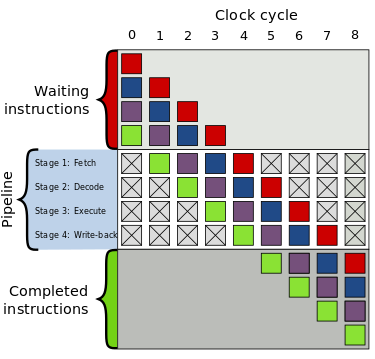
\includegraphics[width=0.4\textwidth]{pipeline}
	\caption{Schemat przykładowego procesora potowego}
	\label{pic:pip}
\end{figure}

Każda instrukcja składa się z czterech mikroinstrukcji. Kolorami (zielony, fioletowy, granatowy, czerwony) są zaznaczone kolejne instrukcje tego procesora, z których każda składa się z czterech mikroinstrukcji. Kolejne kolumny, to cykle procesora. Jak widać, od czwartego cyklu procesor kończy przetwarzanie jednej instrukcji w każdym cyklu, mimo że jedna instrukcja potrzebuje czterech cykli.

}
{W przetwarzaniu potokowym może być wykonywanych kilka instrukcji na raz, lecz te przetwarzanie każdej z tych instrukcji jest na różnych etapach.}

\answer{Sumator jednobitowy}{pozwala uzyskac sumę dwóch liczb jednobitowych z uwzględnieniem przeniesienia z poprzedniej pozycji}{T}
{
Układ kombinacyjny \ref{odp:90}. Implementacja [\ref{pic:sum}]
\begin{figure}
	\centering
	
\includegraphics[width=0.4\textwidth]{sumator}
	\caption{Sumator jednobitowy}
	\label{pic:sum}
\end{figure}

Sumatory wykonane tak jak na rysunku \ref{pic:sum}, można składać ze sobą tworząc sumator n-bitowy.
Dla i-tego sumatora jednobitowego w n-bitowym sumatorze:
\begin{itemize}
	\item wejście $A$, to i-ty bit pierwszego argumentu
	\item wejście $B$, to i-ty bit drugiego argumentu
	\item wejście $C_{in}$ jest podłączone do $C_{out}$ poprzedniego sumatora
	\item wyjście $S$, to i-ty bit sumy
	\item $C_{out}$, to i-ty bit przeniesienia.
\end{itemize}

}
{Służy po temu połączenie $C_{in}$ z $C_{out}$ poprzedniego sumatora}

\answer{Rejestr rozkazów}
{w trakcie wykonywania rozkazu zawartosć rejestru rozkazów musi zmienić się bezpośrednio przed pobraniem argumentu rozkazu z pamięci programu
}{T}
{
	Rejestr przechowujący obecnie przetwarzaną instrukcję. Którą instrukcję trzeba pobrać, określa licznik rozkazów \ref{odp:100}. Rejestr ten jest elementem jednostki sterującej \ref{odp:87} i wykorzystywany przez dekoder rozkazów.
}
{Rozkaz może określać sposób pobierania wartości. Argument nie musi być pobierany z pamięci, może być użyta wartość zachowana w rejestrach. Zastanawiające jest jednak słówko ,,bezpośrednio''.}

\answer{Przykłady układów kombinacyjnych, to}
{żaden z powyższych}{F}
{
	\begin{itemize}
		\item ALU
		\item sumator
		\item komparator
		\item (de)multiplexer
	\end{itemize}
	
}{nie żaden i tyle}

\answer{Przykłady układów sekwencyjnych, to}
{żaden z powyższych}{F}
{
Wszelkiego rodzaju przerzutniki i układy, w których skład one wchodzą (liczniki, rejestry itp.)
	
}{nie żaden i tyle}

\answer{Transmisja asynchroniczna}
{żaden z powyższych}{T}
{
	sposób przesyłania danych pozwalający na nieregularne ich wysyłanie, przy czym początek i koniec transmisji oznaczane są wydzielonym (ustalonym) symbolem.
	
}
{}

\begin{thebibliography}{99}
\bibitem{uw} Marcin Peczarski, \emph{Notatki do wykładu z architektury komputerów}, 17 lutego 2008
\bibitem{js} Notatki do kolosa \url{http://kolos.math.uni.lodz.pl/~archive/Architektura%20komputerow/07%20jednostka%20sterujaca.pdf}
\bibitem{uk} Układ kombinacyjny \url{https://pl.wikipedia.org/wiki/Uk%C5%82ad_kombinacyjny}
\bibitem{sram} Pamięć statyczna RAM \url{http://eduinf.waw.pl/inf/alg/002_struct/0043.php}
\bibitem{dram} Dynamiczna pamięć RAM \url{http://eduinf.waw.pl/inf/alg/002_struct/0044.php}
\bibitem{dwuport} Pamięć dwuportowa \url{https://pl.wikipedia.org/wiki/Pami%C4%99%C4%87_dwuportowa}
\bibitem{licz} Licznik asynchroniczny \url{http://eduinf.waw.pl/inf/alg/002_struct/0035.php}
\bibitem{fpga:hiw} How does an FPGA work? \url{https://embeddedmicro.com/tutorials/mojo-fpga-beginners-guide/how-does-an-fpga-work}
\bibitem{fpga:logi3D} Logi3D \url{http://www.logicbricks.com/Documentation/Flyers/logi3D_Graphics_Accelerator_01.pdf}
\end{thebibliography}

\chapter{Metody numeryczne}
\PartialToc
%\startcontents[chapters]
%\printcontents[chapters]{}{1}{\section*{\contentsname}}

%112
\answer
{EKK\_1, EKK\_7 W pewnym hipotetycznym binarnym systemie zmiennoprzecinkowym zakres danych ujemnych wynosi $<-b,-a>$, chcemy zapisać liczbę $c$, która jest liczbą mniejszą od $-b$ i która ma nieskończone rozwinięcie. W związku z tym zastępujemy ją majbliższą liczbą, którą da się zpisać w tym systemi, czyli liczbą $-b$. Z jakim błędem numerycznym mamy tutaj do czynienia:}
{Błędem obcięcia}
{F}
{Błędem zaokrąglenia}
{}

%113
\answer
{EKK\_1, EKK\_7 Warunkiem koniecznym i wystarczającym zbieżności metod iteracyjnych prostych (takich jak metoda Jacobiego czy metoda Gaussa-Seidla) rozwiązywania układów równań liniowych:}
{Promień spektralny macierzy iterowanej w danej metodzie jest zawsze mniejszy od 1.}
{T}
{}
{}

%114
\answer
{EKK\_1, EKK\_7 Do metod nazywanych metodami dokładnymi rozwiązywania ukłądów równań liniowych zalicza się: }
{Metoda rozkładu LU}
{T}
{\begin{itemize}
\item Metoda Cramera
\item Eliminacja Gaussa
\item Eliminacja Gaussa z wyborem elementu głównego
\item Eliminacja Jordana
\end{itemize}}
{}

%115
\answer
{EKK\_1, EKK\_7 Które z poniżej wymienionych zagadnień numerycznych wykorzystują właściwości przybliżania funkcji wielomianem interpolującym}
{Obliczanie całki oznaczonej funkcji za pomocą kwadratur Newtona-Cotesa}
{}
{}%Całkowanie numeryczne i rozwiązywanie równań rózniczkowych}
{}

%116
\answer
{EKK\_1, EKK\_7 Macierz Hilberta osiąga wysokie wartości współczynnika uwarunkowania(ang. Condition number) na tej podstawie możemy stwierdzić, że:}
{Macierz Hilberta jest zawsze diagonalnie dominująca}
{}
{}
{}

%117
\answer
{EKK\_1, EKK\_7 Wielomiany sklejane (ang. spline) trzeciego stopnia muszą spełniać następujące warunki w punktach sklejań:}
{Ciągłość pierwszej pochodnej funkcji interpolującej}
{T}
{\begin{itemize}
\item Przechodzenie funkcji interpolującej przez węzły interpolacji
\item Ciągłość fukncji interpolującej
\item Ciągłość pierwszej i drugiej pochodnej funkcji interpolującej w punktach sklejań
\end{itemize}}
{W celu znalezienia funkcji interpolującej funkcjami sklejanymi ustalamy przediał $[a,b]$ oraz jego podział węzłami interpolacji takimi, że: $a=x_0<x_1\ldots<x_n=b$ Dane są równieź wartości w węzłach, odpowiednio: $y_0, y_1,\ldots,y_n$. 

Dla $k=0,1,2,\ldots,n-1$ funkcje łączące punkty $(x_{k},y_{k})$ oraz $(x_{k+1},y_{k+1})$ są wielomianami trzeciego stopnia postaci: 
$$s_{k}(x)=a_{k,0}+a_{k,1}(x-x_{k})+a_{k,2}(x-x_{k})^{2}+a_{k,3}(x-x_{k})^{3}\]\[x\in[x_{k},x_{k+1})$$
który ma spełniać następujące warunki:
$$s_{k}(x_{k})=y_{k}; s_{k}(x_{k+1})=s_{k+1}(y_{k+1}); s'_{k}(x_{k+1})=s'_{k+1}(y_{k+1}); s''_{k}(x_{k+1})=s''_{k+1}(y_{k+1})$$
}
%118
\answer
{EKK\_1, EKK\_7 Należy wskazać zdanie prawdziwe dotyczące zagadnienia interpolacji wielomianowej z wykorzystaniem jednomianów (tzw bazy naturalnej):}
{Jest to zadanie źle uwarunkowane}
{T}
{Interpolacja jednomianami jest zagadnieniem źle uwarunkowanym, stąd jej praktyczne zastosowanie jest znikome, chociaż jest najprostszą metodą interpolacji. Macierz bazowa V (Vandermonde'a) jest źle uwarunkowana, więc zwiększenie liczby węzłów interpolacji powoduje znaczny wzrost współczynnika uwarunkowania tej macierzy (niekorzystne ze względów numerycznych).}
{Interpolacja wielomianowa jest szczególnym przypadkiem interpolacji liniowej. Jej zadaniem jest wyznaczenie wielomianu stopnia co najwyżej $n$ przechodzącego przez $n+1$ węzłów interpolacji. Najprostszym wyborem funkcji bazowych jest baza naturalna: $\varphi_0(x)=1, \varphi_1(x)=x, \varphi_2(x)=x^2, \ldots, \varphi_n(x)=x^n$. Funkcja interpolująca ma postać: $F(x)=a_0+a_1x+a_2x^2+\ldots+a_n+x^n$, a układ równań przyjmuje postać:
$$\left[ \begin{array}{ccccc}
1 & x_0 & x_0^2 & \cdots & x_0^n \\
1 & x_1 & x_1^2 & \cdots & x_1^n \\
\vdots & \vdots & \ddots & \vdots \\
1 & x_n & x_n^2 & \cdots & x_n^n
\end{array} \right] \left[ \begin{array}{c}
_0\\
a_1\\
\vdots\\
a_n
\end{array} \right] = \left[ \begin{array}{c}
y_0\\
y_1\\
\vdots\\
y_n
\end{array} \right]$$ }

%119
\answer
{EKK\_1, EKK\_7 Błędy związane z ograniczeniem nieskończonego ciągu wymaganych obliczeń do skończonej liczby działań nazywamy:}
{Błędami nadmiaru (ang. overflow errors)}
{F}
{Błędami obcięcia}
{ }

%120
\answer
{EKK\_1, EKK\_7 Jeśli niewielkie względne zaburzenia danych wejściowych powodują niewielkie względne zmiany wyników to wówczas}
{Współczynnik uwarunkowania osiąga niską wartość}
{T}
{zadanie jest dobrze uwarunkowane}
{Uwarunkowanie zadania możemy mierzyć za pomocą współczynników uwarunkowania zadania. Niska wartość współczynnika świadczy o dobrym uwarunkowaniu, wysoka o złym.}

%121
\answer
{EKK\_1, EKK\_7 Warunkami wystarczającymi, gwarantującymi zbieżność poszukiwania miejsc zerowych funkcji $f(x)$ metodą bisekcji są:}
{Pierwsza i druga pochodna mają stały znak w całym przedziale}
{F}
{\begin{itemize}
\item Funkcja $f(x)$ jest ciągła w przedziale domkniętym $[a,b]$
\item Na końcach przedziału $[a,b]$ wartości funkcji $f(x)$ przyjmują przeciwne znaki, czyli zachodzi 
$f(a)\cdot f(b)<0$
\end{itemize}}
{Przypomnienie: pierwsza pochodna - badanie monotoniczności, druga pochodna - wypukłość funkcji}

% 122
\section{EKK\_1,EKK\_7}
\textbf{Stosując algorytm stycznych poszukiwania jednokrotnego miejsca zerowego funkcji $f(x)$ w przedziale domkniętym $[a, b]$ w dostateczniej bliskości pierwiastka uzyskujemy zbieżność:} \\
\vspace{0.4cm}
\noindent  Kwadratową. \\ Z twierdzenia O rzędzie zbieżności metody Newtona(stycznych): Wykładnik zbieżności metody Newtona (stycznych) wynosi $p^*=2$ w klasie funkcji o zerach jednokrotnych, oraz $p^*=1$ w klasie funkcji o zerach wielokrotnych.

% 123
\section{EKK\_1,EKK\_7}
\textbf{Do całkowania numerycznego używa się m. in. kwadratur Newtona - Cotesa. Do prostych kwadratur Newtona - Cotesa należą:} \\
\vspace{0.4cm}
\noindent  Wzór trapezów. Wzor Simpsona. 

% 124
\section{EKK\_1,EKK\_7}
\textbf{Efekt Rungego jest charakterystyczny dla następujących metod interpolacji: } \\
\vspace{0.4cm}
\noindent Efekt Rungego jest zjawiskiem typowym dla interpolacji za pomocą wielomianów wysokich stopni przy stałych odległościach węzłów, np. interpolacji Lagranga dla węzłów równoodległych. 

% 125
\section{EKK\_1,EKK\_7}
\textbf{Które zdania dotyczące Metody Eliminacji Gaussa rozwiązywania  układów równań są prawdziwe:} \\
\vspace{0.4cm}
\noindent \begin{itemize}
 \item iteracyjne przekształcenie układu równań  $A*x=b$ z macierzą kwadratową do układu postaci $A^nx=b^n$ dla $k=1..n$, który oznacza równoważną postać układu równań w kolejnych etapach przekształceń. 
 \item przekształca macierz do postaci macierzy schodkowej(pierwsze niezerowe elementy kolejnych niezerowych wierszy, znajdują się w coraz dalszych kolumnach, a powstałe wiersze zerowe umieszcza się jako ostatnie)
\end{itemize}

% 126
\section{EKK\_1,EKK\_7}
\textbf{Aby wyeliminować lub znacząco ograniczyć efekt Rungego przy zadaniu iterpolacji można: } \\
\vspace{0.4cm}
\noindent Zastosować interpolację z węzłami gęściej upakowanymi na krańcach przedziału interpolacji.

\chapter{Analiza numeryczna i~symulacja systemów}
\PartialToc
%\startcontents[chapters]
%\printcontents[chapters]{}{1}{\section*{\contentsname}}
\section{EKK\_1}
\textbf{Wskaż prawidłowo sformułowane warunki w zagadnieniach początkowych Cauchy'ego (IVP) dla równania różniczkowego $y'(t) = f(t, y(t)), f: \Omega \subset \Re \times \Re^{n} \shortrightarrow \Re^{n}, t \in [a, b]$.}

\vspace{0.4cm}
\noindent  Warunki początkowe do para $(t_0, y_0) \in \Omega$. Może to być para wektorów, jeśli mamy do czynienia z równaniem wielu zmiennych: $y=[y_1, y_2, ..., y_n]$. Dla wszystkich wartości $y_i$ potrzebujemy wartości początkowych (tj. w punkcie $a$). Wartości na krańcach przedziału są wykorzystywane w zagadnieniach brzegowych (BVP). Odpowiedź przykładowa miesza problem dwóch zmiennych z problemem BVP. 
Przykłady odpowiedzi:
$$n=2, y_{10}=y_1(a), y_{20}=y_2(a)$$
$$n=1, y_0=y(a)$$
%\begin{center}
%
\includegraphics[width=6cm]{buka}
%\captionof{figure}{Buka}
%\end{center}


\section{EKK\_1, EKK\_18}
\textbf{Wskaż diagramy SIMULINK'a, które reprezentują równanie różniczkowe $$y''-2y'+7y=3sin(5t)-1$$}

\vspace{0.4cm}
\noindent Rysunek tłumaczy wszystko. Centralną częścią jest to wielkie kółko. Ono zamyka pętle i wymusza prawdziwość równości. Analogiczny obrazek można zrobić z blokami Derivative (różniczkującymi), ale dla równania $y=\frac{3sin(5t)-1+2y'-y''}{7}$ współczynniki są brzydsze (mało ''naturalne'').
\begin{center}
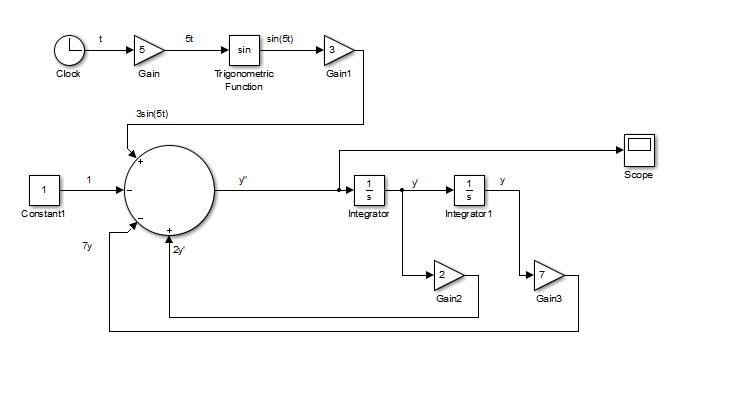
\includegraphics[width=15cm]{08/simulink}
\captionof{figure}{Simulink}
\end{center}
\newpage
\section{EKK\_1}
\textbf{Które zdania odnoszące się do metod rozwiązywania zagadnień początkowych dla równań różniczkowych są prawdziwe?}

\vspace{0.4cm}
\noindent
Metoda trapezowa jest jednokrokowa.\\
Metoda Heuna jest jednokrokowa, dwuetapowa - blok w SIMULINK'u $heun$.\\
Metoda Adamsa-Bashforta jest wielokrokowa, jednoetapowa, jawna.\\
Metoda BDF (Gear'a, wstecznego różniczkowania) jest wielokrokowa, jednoetapowa, jawna - komenda $ode15s$.\\
Metoda Adamsa-Bashforta-Moultona jest wielokrokowa, dwuetapowa - komenda $ode113$.\\
Metoda Milne-Simpsona jest rzadko stosowana ze względu na swój brak stabilności.\\
Obecnie nazwą metody Rungego-Kutty określa się rodzinę jawnych i niejawnych metod wielokrokowych, jak również pewne ich modyfikacje. \\
Tu chodzi o tak zwane metody wielokrokowe (potrzebujemy pamiętać kilka poprzednich stanów, a nie tylko jeden ostatni - dla 6-krokowej metody wzór może wyglądać na przykład tak: $y_{n+1}=y_n+\frac{h}{1440}(4277f_n-7923f_{n-1}+2616f_{n-2}-7298f_{n-3}+2877f_{n-4}-475f_{n-5})+O(h^7)$).
Metoda jednokrokowa korzysta tylko z $y_n$.\\
Metody dwuetapowa korzysta z dwu takich wzorów jak powyższy. Każdy wzór to jeden etap.
Metody niejawne mają po prawej stronie $f_{n+1}$, do którego policzenia potrzebujemy $y_{n+1}$. A $y_{n+1}$ właśnie chcemy policzyć z tego wzoru. No i stąd ta niejawność wzoru.

\section{EKK\_1}
\textbf{Numeryczne rozwiązywanie zagadnienia początkowego. Która metoda jest metodą samostartującą:}

\vspace{0.4cm}
\noindent Eulera, Rungego-Kutty.
Adamsa-Bashforta-Moultona i Geara nie.

\section{EKK\_1}
\textbf{W przypadku metody Eulera zastosowanej do rozwiązywania zagadnienia początkowego dla $y'(t)=f(t,y(t)), y_0=y(0)$ (przy założeniu braku błędu numerycznego wszystkich operacji arytmetycznych)}

\vspace{0.4cm}
\noindent Równanie różniczkowe $\frac{dy}{dx}=f(x,y(x))$ jest liniowe, jeśli $f(x,y(x))=p(x)y+q(x)=Ay+B.$\\
Dla metody Eulera korzystamy z tego, że:$$\frac{dy}{dx}=f(x,y(x)) \Leftrightarrow \frac{y_1-y_0}{h}=f(x,y) \Leftrightarrow y_1-y_0=hf(x,y).$$ To prowadzi do równości $y_{n+1}=y_n+hf(x,y)$.\\
Jak widać przypomina to rozwinięcie Taylora: $y(x_0+h)=y(x_0)+\frac{h}{1!}y'(x_0)+\frac{h^2}{2!}y''(x_0)+\frac{h^3}{3!}y'''(\xi)$, gdzie $\xi \in (x_0, x_0+h)$. Skoro jednak $f(x,y)$ jest funkcją liniową, zatem $y''(x_0)=f'(x,y)\neq0$ w ogólności (np. $f(x,y)=2x$ daje $f'(x,y)=2$). Błąd lokalny pierwszego kroku metody Eulera jest różny od zera, nawet jeśli równanie różniczkowe pierwszego rzędu jest liniowe.\\
Prawdą jest natomiast, że dla metody Eulera błąd lokalny jest proporcjonalny do kwadratu kroku, a błąd globalny - liniowy.

\newpage
\section{EKK\_1}
\textbf{Numeryczne rozwiązywanie zagadnienia początkowego. W metodach typu predyktor-korektor (PECE):}

\vspace{0.4cm}
\noindent Metody PECE to na przykład: Heuna, Adamsa-Bashforta-Moultona, Milne-Simpsona. Predykcja jest częścią jawną, korekcja niejawną. To są dwa etapy. Dlatego te metody są dwuetapowe.\\
Odpowiedź przykładowa, jakoby stosowało się metodę jawną lub niejawną jest nieprawidłowa. Stosuje się zawsze obie metody.

\section{EKK\_1}
\textbf{Które zdania, odnoszące się do metod Rungego-Kutty (RK) rozwiązywania zagadnienia początkowego dla równań różniczkowych, są prawdziwe}

\vspace{0.4cm}
\noindent Odpowiedź przykładowa jest nieprawdziwa. Wersja jawna 4-etapowej metody RK jest różny od wersji niejawnej choćby przez sam fakt istnienia po prawej stronie $f_{n+1}$ (patrz. 8.3.). Istnieją wersje 1-etapowe (to po prostu metoda Eulera), 2-etapowe (Heuna, punktu pośredniego), 4-etapowa jest najczęściej występująca (tę wersję ma się na myśli, gdy mówi się o metodzie RK). 

\section{EKK\_1}
\textbf{Jawne metody Rungego-Kutty (RK). Niech $n_e$ oznacza liczbę etapów metody, a $r$ - maksymalny osiągalny rząd metody.}

\vspace{0.4cm}
\noindent $r<=n_e$.

\section{EKK\_1}
\textbf{Algorytmy optymalizacji statycznej.}

\vspace{0.4cm} Optymalizacja statyczna - szukamy ekstremum funkcji.
Optymalizacja dynamiczna - szukamy ekstremum funkcjonału.\\
Metoda Neldera-Meada jest metodą bezgradientową, bo nie korzysta z pochodnych. Nadaje się więc także do funkcji nieróżniczkowalnych.
Numeryczne metody optymalizacji (deterministyczne): 
\begin{enumerate}
 \item bez ograniczeń:
 \begin{enumerate}
  \item bezgradientowe:
  \begin{itemize}
   \item simpleks Neldera-Meada,
   \item spadku względem współrzędnych (Gaussa-Seidla),
   \item Powella, Rosenbrocka, Hooke'a-Jeevesa;
  \end{itemize}
  \item gradientowe pierwszego rzędu:
  \begin{itemize}
   \item najszybszego spadku,
   \item gradientu sprzężonego;
  \end{itemize}
  \item gradientowe drugiego rzędu i ''superliniowe'':
  \begin{itemize}
   \item Newtona, BFGS,
   \item ''Trust region'';
  \end{itemize}
 \end{enumerate}
 \item z ograniczeniami:
 \begin{itemize}
  \item eliminacji zmiennych,
  \item Lagrange'a,
  \item z funkcją kary,
  \item SQP.
 \end{itemize}
\end{enumerate}

\section{EKK\_1, EKK\_U19}
\textbf{Dyskretna aproksymacja średniokwadratowa. Dla $n+1$ wartości zmiennej niezależnej $x_i, i=1,2,3,...,n, x_i<x_{i+1}$ wykonano pomiary i otrzymano $n+1$ wartości $y_i$. Zależność wielkości mierzonej od $x$ aproksymowano wielomianem $W_m(x)=\Sigma^m_{i=0}a_{i,m}x^i$ z błędem aproksymacji $E_m$. Proszę zaznaczyć prawdziwe implikacje:}

\vspace{0.4cm}
\noindent Aproksymacja oznacza przybliżanie funkcji $y=f(x)$ za pomocą "prostszej" funkcji $y=F(x)$. W zależności od sposobu obliczania błędu aproksymacji, dzielimy je na:
\begin{itemize}
\item jednostajne - błąd liczymy normą Czebyszewa: $ \textpipe\textpipe f-F\textpipe\textpipe =sup_{a<=x<=b}\textpipe\textpipe f(x)-F(x) \textpipe\textpipe ; $
\itemśredniokwadratowe - błąd liczymy: $ \textpipe\textpipe f-F\textpipe\textpipe = \int^{b}_{a}w(x)[f(x)-F(x)]^{2} dx .$
\end{itemize}
Skoro zebrano pomiary w $n+1$ punktach, a aproksymujemy wielomianem $m$-stopnia, to niekoniecznie otrzymamy błąd $E_m>0$. Możliwe jest, że punkty pomiarowe akurat tworzą wielomian $m$-stopnia (zupełnie jak trzy punkty na jednej prostej tworzą wielomian pierwszego stopnia, a nie drugiego). Jednakże implikacja zachodzi w drugą stronę:
$$E_m>0 \Rightarrow n>m.$$

\section{EKK\_1, EKK\_U19}
\textbf{Dla $n+1$ wartości zmiennej niezależnej $x_i, i=1,2,3,...,n,   x_i<x_{i+1}$ wykonano pomiary i otrzymano $n+1$ wartości $y_i$. Zależność wielkości mierzonej od $x$ aproksymowano wielomianem $W_m(x)=\Sigma^m_{i=0}a_{i,m}x^i$. Rozważamy 3 sposoby obliczania błędu aproksymacji $E_m$: 
\begin{enumerate}
\item $E_m=min_{a_0,\ldots,a_m}\Sigma^n_{i=0}\textpipe y_i - W_m(x_i) \textpipe$,
\item $E_m=min_{a_0,\ldots,a_m}\Sigma^n_{i=0}(y_i - W_m(x_i))^2$,
\item $E_m=min_{a_0,\ldots,a_m}max_{i=0,\ldots,n}\textpipe y_i - W_m(x_i) \textpipe$.
\end{enumerate}
Obliczenie współczynników $a_i$ można sprowadzić do zagadnienia liniowego:
}

\vspace{0.4cm}
\noindent Po wpisaniu w wyszukiwarkę Google hasła: ''Zagadnienie liniowe'' otrzymujemy wyniki, które wskazują jednoznacznie na synonimiczność z określeniem: "Programowanie liniowe"(za Wikipedią: ''Programowanie liniowe – klasa problemów programowania matematycznego, w której wszystkie warunki ograniczające oraz funkcja celu mają postać liniową.'').\\
Teraz pokrótce o aproksymacji. Opisano ją w sekcji wyżej, więc wystarczy nadmienić, że szukamy takich współczynników $a_i$, dla których błąd $E_m$ będzie możliwie najmniejszy. \\ 
Okazuje się, że nawet dla aproksymacji średniokwadratowej (opis sekcja wyżej) można sprowadzić problem do programowania liniowego (ciekawych odsyłam do \url{http://kik.weii.tu.koszalin.pl/aproksymacja/aproks_tryg/page_dyp/aprwielpaj.html}). Odpowiedzi 1. i 2. są więc prawidłowe. W przypadku ostatnim można zauważyć, że bierzemy obecny maksymalny błąd $a_i$ i staramy się go zmiejszyć. Norma nie pomaga jednak zwięźle opisać algorytmu (kiedy założyć stop algorytmu, skoro musimy sprawdzić wszystkie możliwe kombinacje, by zminimalizować maksymalne odchylenie?). Wynikałoby z tego, że odpowiedź 3. jest niepoprawna. Warto zaznaczyć, że brak konieczności sprawdzenia wszystkich kombinacji w 1. i 2. wynika z faktu, że szukamy w nich punktu miejsca zerowego pochodnej (optimum). 

\section{EKK\_1}
\textbf{Dla tych samych danych eksperymentalnych:
\begin{center}
\begin{tabular}{l|r r r}
$i$&$0$&$1$&$2$\\
$x_i$&$2$&$4$&$6$\\
$y_i$&$1$&$2$&$1$\\
\end{tabular}
\end{center}
wyznaczono 3 funkcje aproksymujące. W każdym przypadku $k=1,2,3$ funkcja aproksymująca miała postać $f_k(x)=a_kx+b_k$, ale użyto innego kryterium jakości aproksymacji:
\begin{enumerate}
\item \textcolor{blue}{Dla $k=1: min_{a_1,b_1}\Sigma^2_{i=0}\textpipe y_i-f_1(x_i)\textpipe$}
\item \textcolor{red}{Dla $k=2: min_{a_2,b_2}\Sigma^2_{i=0}(y_i-f_2(x_i))^2$}
\item \textcolor{green}{Dla $k=3: min_{a_3,b_3}max_{i=0,1,2}\textpipe y_i-f_3(x_i)\textpipe .$ }
\end{enumerate}
Proszę zaznaczyć prawidłowe odpowiedzi:
}

\vspace{0.4cm}
\noindent Wygląda na to, że obliczenie wszystkich $a_i$ i $b_i$ jest głównym problemem. Chyba dobrym pomysłem jest to narysować:
\begin{center}
\begin{tikzpicture}
\draw (-4,0) -- (4,0) -- (3.7,-0.1)  (3.7,0.1) -- (4,0) (0,-0) -- (0,4) -- (-0.1,3.7)  (0.1,3.7) -- (0,4) ;
\draw [dashed] (2,-1) -- (2,4);
\node at (4,0.3) {x};
\node at (-0.3,4) {y};
\node at (-0.3,0.5) {1};
\node at (-0.3,1) {2};
\node at (1, -0.3) {2};
\node at (2, -0.3) {4};
\node at (3, -0.3) {6};
\coordinate (a) at (1,0.5); \fill (a) circle (2pt);
\coordinate (b) at (2,1);   \fill (b) circle (2pt);
\coordinate (c) at (3,0.5); \fill (c) circle (2pt);
\draw [red] plot (\x, {2/3}); % przeskalowane
\draw [blue] plot (\x, {1/2}); % tu tez przeskalowane
\draw [green] plot (\x, {3/4}); % tu tez przeskalowane
\end{tikzpicture}
\end{center}
\textcolor{red}{Aproksymacja średniokwadratowa} Korzystam z opracowania zalinkowanego sekcję wyżej. Używam notacji użytej tam. Mamy:
$S_0=\Sigma^3_{i=0}x_i^0=3$, $S_1=\Sigma^3_{i=0}x_i^1=12$,$S_2=\Sigma^3_{i=0}x_i^2=56$ oraz $t_0=\Sigma^3_{i=0}x_i^0y_i=4$, $t_1=\Sigma^3_{i=0}x_i^1y_i=16$.
Otrzymujemy równanie macierzowe: 
\[ 
\left[ \begin{array}{cc}
3 & 12 \\
12 & 56 \end{array} \right]
 *
\left[ \begin{array}{cc}
a_0 \\
a_1 \end{array} \right]
=
\left[ \begin{array}{cc}
4 \\
16 \end{array} \right]
 ,\] które daje prostą $y=\frac{4}{3}$.\\
\textcolor{blue}{Aproksymacja jednostajna} Gołym okiem widać rozwiązanie: $y=1$. Jeśli przesunąć prostą w góre lub w dół zwiększy się błąd. Jeśli prosta połączy dwa inne punkty to błąd związany z trzecim będzie dwa razy większy, co też dyskwalifikuje inne rozwiązania. \\
\textcolor{green}{Aproksymacja ''min-max''} Jeszcze bardziej trywialne rozwiązanie: $y=1.5$. Jeśli ktoś nie rozumie dlaczego, powinien zacząć czytać rozwiązanie od nowa.\\

Prawdopodobnie w zadaniu nie chodziło o pamiętanie wzórów i szybkie mnożenie macierzy. To, że wszystkie współczynniki $a_k$ (i równe) wynika z symetrii rozkładu punktów względem prostej $x=4$. Potrzebna jest intuicja, żeby wyczuć która prosta powinna leżeć wyżej.

\section{EKK\_1}
\textbf{Numeryczne metody optymalizacji.
Rozważmy funkcję kwadratową $n$ zmiennych, (w zapisie wektorowym $x=(x_1,x_2,\ldots,x_n)^T$)
$$f(x)=x^TAx+b^Tx+c,$$ gdzie $A$ jest macierzą $n$ \texttimes $n$, $b$ wektorem $n$ \texttimes $1$ o stałych współczynnikach, a $c$ jest skalarem. Załóżmy, że macierz $A$ jest dodatnio określona. Funkcja $f$ ma minimum w punkcie $x_{min}$.
Aby znaleźć minimum tej funkcji mamy do dyspozycji 3 metody: simpleksu Neldera-Meada, najszybszego spadku (steepest descent) oraz Newtona. Startujemy z dowolnego punktu $x \in \Re^n, x \neq x_{min}$. 
}

\vspace{0.4cm}
\noindent Metody najszybszego spadku i Newtona pozwalają na znalezienie minimum w jednym kroku (o ile jesteśmy w zakresie tolerancji dla ekstremum funkcji). Metoda simpleksów musi zawsze przejść kilka kroków (wynika to ze specyfiki działania - znany teren, w którym znajduje się ekstremum i chcemy sprecyzować położenie).

\section{EKK\_1}
\textbf{Dyskretna aproksymacja średniokwadratowa. \\
Czy obliczanie parametrów (współczynników) funkcji aproksymującej można sprowadzić do rozwiązywania układu równań liniowych?
}

\vspace{0.4cm}
\noindent Trzy sekcje wcześniej wyjaśnione zostało, że aproksymacja wielomianowa jest zagadnieniem liniowym. Wątpliwym jest, aby inna klasa funkcji pozwalała na rozwiązanie przez zwykły układ równań. Trzeba pamiętać także, że mówimy o aproksymacji średniokwadratowej bądź jednostajnej.

\section{EKK\_1}
\textbf{Aproksymacja dyskretna.\\
Do aproksymacji zbioru punktów $P_i(x_i, y_i), i=1,2,3,\ldots,n$ używamy funkcji $f(x)$ o parametrach $a_j, j=0,1,\ldots,m $. Stosując 3 różne kryteria jakości aproksymacji (miary błędu aproksymacji):
\begin{enumerate}
\item $k=1: min_{a_0,\ldots,a_m}\Sigma_{i=0}^n\textpipe y_i-f^{(1)}(x_i) \textpipe,$
\item $k=1: min_{a_0,\ldots,a_m}\Sigma_{i=0}^n( y_i-f^{(2)}(x_i) )^2,$
\item $k=1: min_{a_0,\ldots,a_m}max_{i=0,1,\ldots,n}\textpipe y_i-f^{(3)}(x_i) \textpipe.$
\end{enumerate}
otrzymujemy 3 funkcje aproksymujące $f^{(k)}(x), k=1,2,3$ różniące się między sobą tylko wartościami parametrów $a_j, j=0,1,\ldots,m $.\\
Niech $\triangle^{(k)}_{max}$ oznacza odległość (w sensie metryki maksimum)  $k$-tej funkcji aproksymującej $f^{(k)}$ od punktu najbardziej oddalonego, tzn. $\triangle^{(k)}_{max}=max_{i=0,1,\ldots,n}\textpipe y_i-f^{(k)}(x_i) \textpipe$. Proszę zaznaczyć prawdziwe relacje  
}

\vspace{0.4cm}
\noindent $\triangle^{(1)}_{max}\geq\triangle^{(2)}_{max}$ (nie jestem w stanie znaleźć przypadku, dla którego norma średniokwadratowa byłaby mniej "kompromisowa"- liczę na recenzentów w tej kwestii)\\
$\triangle^{(3)}_{max}\leq\triangle^{(1)}_{max}$ i $\triangle^{(3)}_{max}\leq\triangle^{(1)}_{max}$ zawsze, bo 3. kryterium z definicji posiada minimalne maksymalne odchylenie.











\chapter{Języki i technologie webowe}
\PartialToc
%\startcontents[chapters]
%\printcontents[chapters]{}{1}{\section*{\contentsname}}


\vspace{0.4cm}
\noindent
%%%%%%%%%%%% MAGDA :) %%%%%%%%%%%%
\answer{Zaznacz prawdziwe stwierdzenia. Droga pakietu w sieci Internet pomiędzy dwoma węzłami, tj. lista adresów węzłów odwiedzanych przez pakiet...}
{Zależy od dynamicznego routingu}
{T}
{Patrz poniżej}
{\\}
\noindent
Krótkie opowiadanie o rutowaniu.\\

Routing jest to należący do warsty 3 proces kierowania pakietów IP poprzez sieć tak, aby osiągneły one swój 
docelowy węzeł (identyfikowany poprzez Adres IP).\\
Router jako urządzenie odpowiedzialne za proces routingu odbiera pakiety IP i decyduje o tym, dokąd (na który podłączony do niego fizycznie interfejs, a) zostaną przesłane. Owy pakiet IP zawiera w sobie m.in. informację o odbiorcy (adres IP węzła docelowego) oraz wartość TTL (ang. Time To Live) bądącą liczbą przeskoków jaką jest w stanie stolerować pakiet przed uznaniem go za zaginiony. Router do wykonania swojego zadania posługuje się tablicą rutowania, w której to zapisane ma dokąd przesłać pakiet o danej adresacji. Zawartość owej tablicy rutowania jest wynikiem pracy protokołów rutowania (nie mylić z rutowalnymi/rutowanymi), które to dziela się na statyczne i dynamiczne.\\
Rutowanie statyczne polega na uzupełnieniu tablicy rutowania przez administratora. W takiej sytuacji rutery zawsze wybierają dla pakietu tę drogę, którą nakazał im administrator i w razie awarii części sieci nie mogą samodzielnie wybrać innej. W przypadku rutowania dynamicznego,  rutery samodzielnie zbierają informacje (np odległość do celu, przepustowość łącza, obciążenie łącza, koszt łącza) i aktualizują zapisy w tablicy; w razie tłoku lub awarii ruter sam decyduje o wybraniu dla pakietu alternatywnej drogi. 

W ten sposób pakiet danych przechodzi pomiędzy kolejnymi sieciami. Takie kolejne przejście
nazywane jest przeskokiem lub hop-em. W tym rozumieniu tablica rutingu zawarta w ruterze lub w
komputerze sieciowym zawiera właśnie przyporządkowania adresów IP dotyczące jednego hopu.\\
Równolegle do protokołu IP w warstwie 3 działa jego rozszerzenie ICMP – Internet Control Message Protocol. Stworzone zostało ono do celów diagnostyki połączeń IP oraz routingu. ICMP posługuje się komunikatami typu “Żyjesz? Żyję”, jak również rozsyłaniem informacji o przekroczeniu czasu życia pakietu na podstawie wartości TTL. ICMP jest więc prawa ręką wszystkich dynamicznym protokołów rutowania.\\ \\


Wnioski i zdania prawdziwe dla "drogi pakietu w sieci Internet pomiędzy dwoma węzłami":
\begin{itemize}
\item Droga pakietu jest bespośrednim efektem procesu rutowania; nie jest jednak zapamiętywana 
\item Długość tej drogi jest liczbą przeskoków pakietu, gdzie przeskokiem jest każdy router, przez który musi zostać przesłany pakiet aby osiągnąć swoją destynację.
\item W przypadku rutowania statycznego droga pakietu z A do B będzie zawsze taka sama
\item W przypadku rutowania dynamicznego droga pakietu z A do B może sie zmieniać - algorytm wybranego protokołu może zaproponowac inną, bardziej optymalną drogę na skutek zmian obciążenia sieci lub powstania ustarek
\item Podczas rutingu przekazanie pakietu do kolejnego węzła jest zawsze równoważne zmniejszeniu o 1 (jeden) wartości jego TTL (dokładniej: wartość TTL pakietu jest zmiejszana przez kolejny ruter, który został jego odbiorcą)
\item Jedną z metod sprawdzenia przemirzanej przez pakiet drogi z A do B jest zastosowanie narzędzia traceroute; traceroute działa na zasadzie rozsyłania pakietów zaadresowanych na B i przydzielaniu im różnym TTL, a następnie wyciagania wniosków z powracającyh komunikatów ICMP.
\end{itemize}


\vspace{0.4cm}
\noindent
Poprzedni opis: \\
Droga takiego pakietu zależy od stanu tablic routingu. Jeżeli stosowany jest routing dynamiczny wtedy pierwsza próba wysłania pakietu się nie powiedzie - router nie zna adresu mac celu i musi go odnaleźć w związku z czym porzuca pakiet, natomiast jeśli w tablicy routingu znajduje się już adres mac węzła docelowego pakiet pójdzie dalej. Całość oczywiście zależy od stopnia skomplikowania sieci (np. ilość routerów po drodze).
\\
\\
Ścieżka pakietu w prostej sieci jest bardzo fajnie i obrazowo opisana tutaj:\\
http://jaredheinrichs.com/tracing-packet-flow-between-a-2-switches-and-a-router.html



\vspace{0.4cm}
\noindent 
%%%%%%%%%%%% MAGDA :) %%%%%%%%%%%%
\answer{Serwery DNS oferują:}
{Translację nazw symbolicznych adresów poczty elektronicznej do nazw symbolicznych węzłów obsługujących te adresy}
{T}
{Patrz poniżej}
{Serwery DNS są między innymi odpowiedzialne za przechowywanie informacji specyficznych dla systemu dostarczania poczty, nazywanych rekordami MX. Rekord MX (ang. Mail eXchanger) precyzuje który host (lub grupa hostów) odbiera pocztę dla poszczególnych domen. Jeżeli nasza domena nie zawiera rekordu MX w systemie DNS przesyłki będą dostarczane bezpośrednio do naszego hosta, pod warunkiem że nasz host posiada w systemie DNS rekord A odzwierciedlający nazwę naszego hosta na odpowiadający jej numer IP. \\

Serwery DNS (Domain Name System) są znane głównie z translacji nazw symbolicznych na adresy IP oraz translacji odwrotnej (Reverse Lookup). Zawarte jednak pola w rekordach odpowiedzi DNS niosą dodatkowe informacje, co oznacza, że serwery DNS mogą mieć w swojej ofercie nieco więcej niż wspomniano powyżej.\\}

\vspace{0.4cm}
Najważniejsze typy rekordów DNS oraz ich znaczenie względem treści pytania:
\begin{description}
\item[A] adres hosta (ipV4) - translacja na adres IP
\item[AAAA]  adres hosta (ipV6) 
\item[PTR]  	
	rekord wskaźnika - mapuje adres IPv4 lub IPv6 na nazwę kanoniczną hosta. 		Określenie rekordu PTR dla nazwy hosta (ang. hostname) w domenie in-addr.arpa 	(IPv4), bądź ip6.arpa (IPv6), który odpowiada adresowi IP, pozwala na 			implementację odwrotnej translacji adresów DNS (ang. reverse DNS lookup) 
\item[MX] mapuje nazwę domeny DNS na nazwę serwera poczty oraz jego priorytet 
\item[CNAME]	alias nazwy domeny. Wszystkie wpisy DNS oraz poddomeny są 	poprawne także dla aliasu 
\item[TXT]	rekord ten pozwala dołączyć dowolny tekst do rekordu DNS 
\item[NS] Name Server, serwer nazw dla danej strefy 
\item[SOA]    rekord adresu startowego uwierzytelnienia (ang. start of authority record) ustala serwer DNS dostarczający autorytatywne informacje o domenie internetowej 
\end{description}


Narzędzia do odpytywania DSN (poza niewidocznym modułem przeglądarki): host, dig\\




\vspace{0.4cm}
\noindent 
%%%%%%%%%%%% MAGDA :) %%%%%%%%%%%%
\answer{Zaznacz prawdziwe stwierdzenie. Protokół HTTP w wersji 1.1...}
{Umożliwia transmisję danych nieprzekraczających 2kB}
{F}
{Protokół HTTP nie okresla maksymalnej długości URI. Istnieje jedynie ograniczenie narzucone przez przeglądarki (rózne dla roznych przeglądarek), dlatego bezpiecznie  jest zakładać, że jest ono równe 2kB.}
{\\}

\textsc{\textbf{wybrane różnice między wersją HTTP 1.0 i 1.1}}
\begin{itemize}

\item{\textbf{w  1.1 w zapytaniu trzeba określić hosta docelowego}\\
GET / HTTP/1.1 \\
Host: kis.agh.edu.pl}
\item \textbf{HTTP 1.1 pozwala na "trwałe połączenia"} \\ 
Oznacza to, że można zrealizować więcej zapytań w ramach jednego otwartego połączenia. W 1.0 każde połaczenie było zamykane po każdej wymianie zapytanie-odpowiedź i musiało być otwarte na nowo dla każdego kolejnego zapytania. W celu zlikwidowania tego problemu HTTP/1.0 wprowadziło rozszerzenie - nagłówek Keep-Alive. W HTTP/1.1 ten nagłówek nie jest potrzebny, gdyż połączenia Keep-Alive są domyślne (zachowanie zmienia Connection: close).

\item \textbf{Wersje 1.0 i 1.1 różnią się sposobami cache'owania.} \\
HTTP 1.0 wspierał cache za pomoca headera "If-Modified-Since". HTTP 1.1 rozszerza możliwości cacheowania wprowadzając 'entity tag' - kiedy dwa zasoby są identyczne, bądą one miały jednakowe entity tags. HTTP 1.1 dodaje równiez nowe warunkowe headery: If-Unmodified-Since, If-Match, If-None-Match.

\item \textbf{HTTP/1.1 wprowadza nowy kod/status zwrony: 100 Continue.} \\
Zapobiega on sytuacji w której klient wysyła duże zapytanie do serwera nie będac pewnym, czy jest autryzowany do wykonania takiego zapytania lub też czy serwer jest w stanie takie zapytanie przetworzyć. W Kttp/1.1 klient moze więc wysłaż zapytanie z samymi nagłówkami, and the server will tell the client 100 Continue, go ahead with the body.

\item \textbf{HTTP/1.1 wprowadza metodę "OPTIONS".} \\
Pozwala ona klientowi HTTP na określenie możliwości serwera HTTP. 
\end{itemize}

\vspace{0.2cm}
\noindent
Ogólnie na temat protokołu HTTP: \\
Podobnie jak większość protokołów sieciowych, HTTP używa modelu klient-serwer: klient HTTP otwiera połączenie i wysyła komunikat żądania do serwera HTTP. Serwer następnie zwraca komunikat odpowiedzi, zwykle zawierający zasób, o który został poproszony.
Portem zarezerwowanym dla HTTP jest 80 port TCP oraz rzadziej używane porty 8008 i 8080.\\

\textsc{\textbf{Struktura protokołu HTTP}}

\begin{enumerate}
\item Żądanie
	\begin{enumerate}
	\item{polecenie}
	\item{nagłówki (0 lub więcej)}
	\item pusta linia
	\item dane
	\end{enumerate}
\item Odpowiedź
	\begin{enumerate}
		\item pojedyncza linia statusu: \textit{protokół kod opis}
		\item{nagłówki (0 lub więcej)}
		\item pusta linia
		\item dane
	\end{enumerate}
\end{enumerate}


\textsc{\textbf{Kody statusu}}

\begin{description}
\item[1xx] powiadomienie
\item[2xx] powodzenie – 200 OK
\item[3xx] przekierowanie do innego URI – 301 Moved Permanently
\item[4xx] błąd po stronie klienta – 404 Not Found
\item[5xx] błąd po stronie serwera – 500 Server Error
\end{description}

\textsc{\textbf{metody http}}
\begin{description}

\item[OPTIONS] — pozwala klientowi ustalić opcje i/lub wymagania związane z danym zasobem, albo możliwości danego serwera, nie implikując działań zasobu i nie inicjując pobierania zasobu.
\item[GET] — pobiera informacje zidentyfikowane przez URI, do którego zostało zgłoszone żądanie. Jeżeli URI zidentyfikuje proces wytwarzający dane, to wytworzone dane zostaną zwrócone jako jednostka.

\item[HEAD] — identyczny z GET, z tym że serwer nie zwraca w odpowiedzi treści komunikatu. Metoda ta uzyskuje informacje dotyczące jednostki nie przesyłając samej treści jednostki i jest wykorzystywana do testowania ważności, dostępności oraz niedawnych modyfikacji łączy hipertekstowych.

\item[POST] — żąda, aby serwery przyjmowały jednostkę załączoną w żądaniu,  POST jest wykorzystywany do przypisywania zasobów, do wysyłania komunikatów, do przedkładania danych formularzy, itp.

\item[PUT] — żąda, aby jednostka załączona w żądaniu została zapamiętana pod URI, do którego zostało zgłoszone żądanie. Jeżeli dany zasób wspomniany w URI już istnieje, to przesyłaną jednostkę uznaje się za wersję zmodyfikowaną. Jeżeli URI nie wskazuje na istniejący zasób, a żądający użytkownik może zdefiniować URI jako nowy zasób, to zasób jest tworzony na serwerze.

\item[DELETE] — żąda, aby serwer usunął zasób zidentyfikowany przez URI.

\item[TRACE] — wywołuje zdalną pętlę zwrotną komunikatu żądania. Ostateczny odbiorca żądania odbija otrzymany komunikat z powrotem do klienta. TRACE pozwala klientowi zobaczyć co jest odbierane na drugim końcu łańcucha żądania. Informacja ta może być wykorzystywana do testowania, lub znajdywania uszkodzeń.

\item[CONNECT] — nazwa metody zarezerwowana do wykorzystywania wraz z proxy, który może dynamicznie przełączyć się na pełnienie funkcji tunelu, przy użyciu, na przykład, tunelowania z wykorzystaniem warstwy zabezpieczeń łączy (SSL). Proxy to program pośredniczący, pełniący zarówno funkcję serwera, jak i klienta, w celu zgłaszania żądań w imieniu innych klientów.
\end{description}

\textsc{\textbf{nagłówki}}\\
Z wykładu:
\begin{description}

\item[Klient:] \hfill \\
	\begin{description}
	\item[From]: – zwykle email
	\item[User-Agent:] – identyfikacja klienta: Nazwa/Wersja Host: – HTTP 1.1
	\end{description}
\item[Serwer:] \hfill \\
	\begin{description}
		\item[Server:] - analogicznie jak User-Agent
		\item[Last-Modified:] – Data i godzina modyfikacji zasobu 
		\item[Connetion:] – rodzaj połączenia (close dla HTTP 1.0)
		\item[Content-Type:] – tym MIME, np. text/html, application/octet-stream
		\item[Content-Length:] – rozmiar w bajtach
	\end{description}
\end{description}
\href{http://www.wikiwand.com/pl/Lista_nag%C5%82%C3%B3wk%C3%B3w_HTTP}{Więcej nagłówków: wiki} 
\\




\vspace{0.4cm}
\noindent 
%%%%%%%%%%% MAGDA :) %%%%%%%%%%%%%
\answer{Do bezpośredniej komunikacji z serwerem WWW służą następujące narzędzia}
{nc}
{T}
{Patrz poniżej:}
{\\}

Bezpośrednią komunikację z serwerem WWW umożliwiają:
\begin{itemize}
\item{nc (netcat)} 
\item{curl} 
\item{wget} 
\end{itemize}

\vspace{0.2cm}
\noindent
Uwaga1: Wymienione narzędzia to te, które pojawiły sie w stosownej laborce "http", jednak prowadzący również informuje, że "Istnieje wiele innych pożytecznych narzędzi dla protokołu HTTP".\\

\vspace{0.2cm}
\noindent
Uwaga2: w poprzedniej wersji istnieje odpowiedź "każdy klient protokołu zdalnego logowania (ssh, telnet)" - nie jestem co do niej przekonana; według mnie komunikacja z serwerem WWW nie jest równoważna zdalnemu logowaniu.\\
Review: Zgadzam się z tą opinią.
 


\vspace{0.4cm}
\noindent
%%%%%%%%%%% MAGDA :) %%%%%%%%%%%%%
\answer{Wskaż prawdziwe stwierdzenia~o poniższym fragmencie kodu XHTML 1.0 Strict:\\
\centerline{<p><a href=http://www.agh.edu.pl><br></p>}}
{Nie jest poprawny, element br nie posiada znacznika zamykającego}
{T}
{Patrz poniżej}
{\\}
\noindent
Prawdziwe stwierdzenia na temat powyższego fragmentu kodu:
\begin{itemize}
\item Nie jest poprawny, element br nie posiada znacznika zamykającego - w XHTML wszystkie znaczniki muszą być zamknięte
\item Nie jest poprawny, wyrażenie  http://www.agh.edu.pl  powinno zostać ujęte~w cudzysłów.  
\item Nie jest poprawny, element a nie posiada znacznika zamykającego; mógłby on został naprawiony na dwa sposoby:
	\begin{itemize}
    \item <a href=http://www.agh.edu.pl />
    \item <a href=http://www.agh.edu.pl> AGH </a>
    \end{itemize}
\end{itemize}



\vspace{0.4cm}
\noindent
%%%%%%%%%%%%%%%%%%%%%%%%%%%%%%%%%%%%%%%%%%%%%%%%%%%%%%%%%%%%%%%%%%%%%%%%%%%%%%%%%%%%%%%%%%
%%% PYTANIE 147

\section{Dany jest poniższy fragment kodu XHTML 1.0 Strict. Obrazek i.jpg ma rozmiary 1024x768. Zaznacz prawdziwe stwierdzenia.}
\begin{lstlisting}[language=html,frame=single]
  <img src="http://www.agh.edu.pl/i.jpg"
       width="320"
       height="240"
       alt="logo AGH" />
\end{lstlisting}
\textbf{Przykładowa odp:} Kod powoduje przeskalowanie obrazka po stronie przeglądarki. \textbf{PRAWDA}


\vspace{0.2cm}
\noindent
\textbf{Zdania prawdziwe na temat elementu $<img />$ w XHTML 1.0:}
\begin{itemize}
\item znacznik końca jest niedozowolony
\item najważniejsze dostępne atrybuty: src, alt, height, width, longdesc
\item szerokość i wysokość może zostać podana w pikselach jaki i w $\%$ (domyślnie w px)
\item obrazki pobierane są w ich oryginalnej rozdzielczości i skalowane po stronie przeglądarki
\end{itemize}

%%%%%%%%%%%%%%%%%%%%%%%%%%%%%%%%%%%%%%%%%%%%%%%%%%%%%%%%%%%%%%%%%%%%%%%%%%%%%%%%%%%%%%%%%%
%%% 148
\answer{Ile zasobów z dyrektywami CSS może być skojarzonych z pojedynczym dokumentem XHTML 1.0 Strict?}
{Zero}
{F}
{Nie ma ograniczenia ilości dołączanych plików styli.}
{Możemy skojarzyć wiele zasobów np. dla różnych typów mediów (screen, print) definiujemy osobne zasoby}

%%%%%%%%%%%%%%%%%%%%%%%%%%%%%%%%%%%%%%%%%%%%%%%%%%%%%%%%%%%%%%%%%%%%%%%%%%%%%%%%%%%%%%%%%%
%%% PYTANIE 149
\section{Zaznacz prawdziwe stwierdzenia dotyczące poniższego kodu CSS 2.1.}
\begin{lstlisting}[language=html, frame=single]
  .nav > div {
      color: white;
      background: #119500;
      float: right;
      width: 120px;
      padding: 1px;
      font-size: small;
      border: solid red 1px;
  }
\end{lstlisting}

\noindent
{\textbf{Przykładowa odpowiedź:}}
Kolor tła ustalony jest jako wartości składowych RGB, odpowiednio (dziesiętnie) 11, 95, 0.
\textbf{FAŁSZ}

\vspace{0.4cm}
\noindent
\textbf{Odpowiedź:}
Brak jednoznacznej odpowiedzi.

\vspace{0.4cm}
\noindent
\textbf{Wyjaśnienie:}

\noindent
Powyższa definicja styli dotyczy elementu $div$, będącego bezpośrednim potomkiem elementu z klasą $nav$ (znaczenie selektora \textbf{>}).
Na przykład:
\begin{lstlisting}[language=html, frame=single]
<div class="nav">
    <div id="stylowanyDiv"></div>
</div>
\end{lstlisting}

\noindent
Tu stylowanie nie będzie miało miejsca:

\begin{lstlisting}[language=html, frame=single]
<div class="nav">
    <span>
        <div id="nieBedeStylowany"></div>
    </span>
</div>
\end{lstlisting}


\begin{itemize}
\item
\textbf{color} - kolor tekstu wewnątrz elementu; w tym przypadku tekst będzie BIAŁY.
\item
\textbf{background} - tło elementu; tutaj ustawiony kolor tła jako wartość HEX koloru. Chcąć ustawiać kolor jako dziesiętne wartości RGB używamy formy rgb(R, G, B)
\item
\textbf{float} - w najprostszej formie określa czy i jak element będzie 'opływany' przez tekst; tutaj, div będzie znajdował się po prawej stronie, a tekst z lewej.
\item
\textbf{width} - szerokość elementu blokowego; tutaj, 120 px
\item
\textbf{padding} - jest odstępem między zawartością elementu a jego wewnętrzną krawędzią; tutaj, 1px dla wartości górnej, prawej, dolnej i lewej jednakowo.
\item
\textbf{font-size} - rozmiar tekstu; tutaj, mniejsza niż domyślna. Dokładny rozmiar jest zależny od przeglądarki.
\item
\textbf{border} - obramowanie elementu; solid - linia ciągła, red - czerwony kolor obranowania, 1px - grubość obramowania;
\end{itemize}
\begin{center}
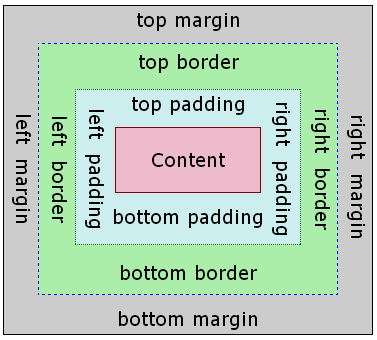
\includegraphics[width=6cm]{09/boxmodel}
\captionof{figure}{Model pudełkowy elementów strony}
\end{center}

\noindent
\textbf{!UWAGA!: }120px jest poprawne; 120 px już nie!

%%%%%%%%%%%%%%%%%%%%%%%%%%%%%%%%%%%%%%%%%%%%%%%%%%%%%%%%%%%%%%%%%%%%%%%%%%%%%%%%%%%%%%%%%%
%%% PYTANIE 150
\section{Wskaż prawdziwe stwierdzenia odnośnie poniższego fragmentu kodu PHP.}
\begin{lstlisting}[language=php, frame=single]
$fp = fopen("plik_do_blokowania", "r+");
if(flock($fp, LOCK_EX)) {
    processing();
    flock($fp, LOCK_UN);
} else {
    problem();
}
fclose($fp);
\end{lstlisting}

\noindent
{\textbf{Przykładowa odpowiedź:}}
Funkcja \textit{processing()} jest wywoływana w sekcji krytycznej.
\textbf{PRAWDA}

\vspace{0.4cm}
\noindent
\textbf{Odpowiedź:}
Brak jednoznacznej odpowiedzi.

\vspace{0.4cm}
\noindent
\textbf{Wyjaśnienie:}

\begin{enumerate}
\item 
Funkcja \textit{fopen} przyjmuje jako pierwszy argument ścieżkę do pliku, który ma zostać otwarty, a jako drugi - tryb otwarcia, jak niżej:
\begin{itemize}
\item
\textbf{r} - otwiera plik do odczytu
\item
\textbf{r+} - otwiera plik do odczytu i zapisu
\item
\textbf{w} - kasuje zawartość pliku i otwiera go do zapisu
\item
\textbf{w+} - kasuje zawartość pliku i otwiera go do zapisu i odczytu
\item
\textbf{a} - otwiera plik do dopisywania
\item
\textbf{a+} - otwiera plik do dopisywania i odczytu
\end{itemize}
Zwraca wartość liczbową identyfikującą otwarty plik.
\item
Funkcja \textit{fclose} służy do zamknięcia pliku otwartego wcześniej przez fopen. Jako argument przyjmuje liczbowy identyfikator pliku, który ma zostać zamknięty.
\item
Funkcja \textit{flock} służy do zarządzania blokowaniem dostępu do pliku jako zabezpieczenie podczas współdzielenia pliku. Zapobiega to równoczesnej modyfikacji pliku przez kilka osób/wątków.
\begin{itemize}
\item
\textbf{LOCK\_SH} - dostęp do odczytu; inne wątki mogą czytać plik, ale nie mogą zablokować go do zapisu. Zapobiega to odczytowi niepełnych danych przez inne wątki i wprowadzeniu zmian w pliku czytanym przez inne wątki.
\item
\textbf{LOCK\_EX} - dostęp do zapisu; wątek blokując plik w ten sposób ma go 'na wyłączność'. Inne wątki nie mogą go odczytać, a tym bardziej zapisać. Zapobiega wprowadzaniu zmian przez kilka wątków jednocześnie oraz odczytania niepełnych (przed edycją) danych.
\item
\textbf{LOCK\_UN} - zwolnienie blokady 
\item
\textbf{LOCK\_NB} - Gdy ustawiona, proces który natknął się na blokadę nie będzie czekał na swoją kolej. Używa się tej opcji w połączeniu, z którąś opcją blokady np. \textit{flock(\$fp, LOCK\_EX | LOCK\_NB)}. Użyta w naszym przypadku pozwoliła by na przejście bo bloku \textit{else} gdy plik jest już zablokowany, zamiast czekać na zwolnienie.\textbf{LOCK\_UN}
\end{itemize}
\textit{flock} zwraca true w przypadku sukcesu i false w przeciwnym razie.
Gdy \textit{flock} nie może uzyskać do zasobu, oczekuje na zwolnienie blokady przez inny wątek!

Funkcja \textit{flock} może przyjmować także opcjonalnie trzeci parametr. Jego wartość jest ustawiana jako 1, gdy proces zostanie zablokowany (nie uzyska dostępu do pliku). Głównie służy do sprawdzenia czy coś złego się nie wydarzyło - gdy funkcja zwraca \textbf{false}, a trzeci parametr ma wartość 0, oznacza to że wystąpił jakiś błąd, ponieważ \textit{flock} nie mógł uzyskać blokady, a jednak proces nie został wstrzymany przez już istniejącą blokadę na pliku.
\end{enumerate}


\textbf{Analiza kodu:}
\begin{enumerate}
\item
Otwieramy plik "plik\_do\_blokowania" w celu odczytu i zapisu. Identyfikator przypisujemy do zmiennej \$fp.
\item
Następnie próbujemy uzyskać dostęp do pliku w trybie exclusive.
Jeżeli plik nie został wcześniej zablokowany ani do odczytu, ani zapisu przez inny wątek - funkcja \textit{flock} zwraca \textbf{true} i blokuje plik.
\item
Wówczas wchodzimy w sekcję krytyczną gdzie aktywowana jest funkcja \textit{processing()}.
\item
Po jej wykonaniu blokada pliku jest zwalniana poprzez \textit{flock(\$fp, LOCK\_UN)}.
\item
Jeżeli plik jest odczytywany lub zapisywany przez inny wątek (został wcześniej zablokowany) funkcja \textit{flock} zwraca \textbf{false}.
Wówczas \textit{flock} oczekuje na zwolnienie blokady przez inny wątek; czeka na swoją kolej.
\item
Po wykonaniu powyższych czynności plik zostaje zamknięty.
\end{enumerate}

\noindent
\textbf{!Uwaga!: }Tak naprawdę, w tym przykładzie nie wejdziemy do bloku 'else'! (chyba, że coś złego wydarzy przy próbie blokowania)

%%%%%%%%%%%%%%%%%%%%%%%%%%%%%%%%%%%%%%%%%%%%%%%%%%%%%%%%%%%%%%%%%%%%%%%%%%%%%%%%%%%%%%%%%%
%%%% Pytanie 151
\section{Zawartość poniższego formularza przesłano do skryptu PHP. Zaznacz prawdziwe stwierdzenia.}
\begin{lstlisting}[language=html, frame=single]
<form action="skrypt.php" method="post" enctype="multipart/form-data">
    <p>
        <input type="file" name="plik"/>
        <input type="text" name="comment" />
        <input type="submit" value="wyslij" />
    </p>
</form>
\end{lstlisting}

\noindent
{\textbf{Przykładowa odpowiedź:}}
W zmiennej \textit{\$\_POST['comment']} będzie dostępna zawartość pola tekstowego.
\textbf{PRAWDA}

\vspace{0.4cm}
\noindent
\textbf{Odpowiedź:}
Brak jednoznacznej odpowiedzi.

\vspace{0.4cm}
\noindent
\textbf{Wyjaśnienie:}
Formularz php składający się z trzech elementów:
\begin{enumerate}
\item
Kontrolka do uploadu pliku. Klikając klawisz pojawi się okno eksploratora i można wybrać plik z dysku. Zmienna z nim związana nazwana została 'plik'.
\item
Pole tekstowe, umożliwiające wpisanie tekstu przez użytkownika. Pierwotnie pole tekstowe jest puste. Zmienna z nim związana nazwana została 'comment'.
\item
Klawisz zatwierdzający formularz. Po jego wciśnięciu dane z formularza zostają wysłane do skryptu 'skrypt.php' metodą POST.
\end{enumerate}

Parametr \textbf{enctype} określa w jaki sposób dane z formularza zostaną przekształcone. Może być użyty TYLKO w połączeniu z \textbf{method="POST"}.
	Możliwe wartości:
\begin{itemize}
\item
\textbf{application/x-www-form-urlencoded} - DOMYŚLNE; Wszystkie dane są przekształcane. Spacje zmieniane na +, znaki specjalne zmieniane na wartości ASCII HEX.
\item
\textbf{multipart/form-data} - żadne znaki nie są przekształcane; wymagany w przypadku użycia w formularzu kontrolki typu \textbf{'file'}
\item
\textbf{text/plain}- spacje są przekształcane na znak +, znaki specjalne nie są przekształcane
\end{itemize}

Po stronie skryptu php dostępne są wartości z tablicy asocjacyjnej \textit{\$\_POST} (pola z formularza z metodą \textbf{POST}; przy użyciu metody \textbf{GET} wartości dostępne są spod \textit{\$\_GET}) oraz \textit{\$\_FILES} (dane z kontrolki typu \textbf{file}).

\begin{itemize}
\item
\$\_POST: Array ([comment] => <tresc\_komentarza\_wpisana\_w\_polu>)
\item
\$\_FILES: Array ([plik] => Array ([name] => <nazwa\_pliku> [type] => image/png [tmp\_name] => <sciezka\_do\_pliku\_w\_tempie> [error] => 0 [size] => 38676))
\end{itemize}
Do elementów dostać się można na przykład: \textit{\$\_POST['comment']}, \textit{\$\_FILES['plik']['name']}.

Elementy formularza zgrupowane są wewnątrz znacznika akapitu (<p>).

%%%%%%%%%%%%%%%%%%%%%%%%%%%%%%%%%%%%%%%%%%%%%%%%%%%%%%%%%%%%%%%%%%%%%%%%%%%%%%%%%%%%%%%%%%
%%%% Pytanie 152
\section{Co jest efektem działania poniższego programu~w języku PHP.}
\begin{lstlisting}[language=php, frame=single]
<?php
    $wiek = array('ala'  => 12, 'ela' => 22, 'franek' => 54);
    foreach ($wiek as $k =>$w)
        echo $k.' '.$w."\n";
?>
\end{lstlisting}
{\textbf{Przykładowa odpowiedź:}}
Wygenerowanie na standardowym wyjsciu m.in. wartości komórek z tablicy  \textit{\$wiek}.
\textbf{PRAWDA}

\vspace{0.4cm}

\noindent
\textbf{Wyjaśnienie:}\\
\noindent
Tablice~w PHP działają jak mapy, mają pary kluczy wraz~z wartościami.~W związku~z tym zostanie wypisany następujący ciąg:
\begin{lstlisting}[language=html,frame=single]
  ala 12
  ela 22
  franek 54
\end{lstlisting}
\vspace{0.4cm}

%%%%%%%%%%%%%%%%%%%%%%%%%%%%%%%%%%%%%%%%%%%%%%%%%%%%%%%%%%%%%%%%%%%%%%%%%%%%%%%%%%%%%%%%%%
%%%% Pytanie 153
\section{Jak długi będzie czas wykonania poniższego programu napisanego w języku PHP?}
\noindent
\textbf{Zakłada się, że program uruchamiany jest jako aplikacja WWW tj. dostępny jest pod określonym adresem URI, a interpreter PHP uruchamiany jest przez serwer WWW.}

\begin{lstlisting}[language=php,frame=single]
<? php
    echo 'start';
    sleep(6);
?>

\end{lstlisting}
{\textbf{Przykładowa odpowiedź:}}
Dokładnie 6 sekund.
\textbf{FAŁSZ}

\vspace{0.4cm}
\noindent
\textbf{Odpowiedź:}
Dłużej niż 6 sekund.
\vspace{0.4cm}

\noindent
\textbf{Wyjaśnienie:}\\
\noindent
Wywołanie \textbf{sleep(6)} powoduje "uśpienie" programu na 6 sekund. Do tego czasu należy doliczyć także czas wykonania instrukcji \textbf{echo 'start'}, więc ogólny czas wykonania programu będzie większy niż 6 sekund. Sprawdzone za pomocą funkcji \textbf{microtime()}.

\vspace{0.4cm}
\noindent

%%%% Pytanie 154
\section{Która~z poniższych metod~w języku JavaScript zwraca element~o unikalnym identyfikatorze \textit{form}?}
\noindent
{\textbf{Przykładowa odpowiedź:}}
\begin{lstlisting}[language=html]
document.getElementByUId('form');
\end{lstlisting}
\textbf{FAŁSZ}

\vspace{0.4cm}
\noindent
\textbf{Odpowiedź:}
\begin{lstlisting}[language=html]
document.getElementById('form');
\end{lstlisting}


%%%% Pytanie 155
\section{Zaznacz prawdziwe stwierdzenia dotyczące poniższego kodu~w języku JavaScript}

\begin{lstlisting}[language=html, frame=single]
car = new Array();
car[0] = new Object();
car[0].make = 'Fiat';
car[0].vin = '123';
car[1] = new Object();
car[1].make = 'Ford';
car[1].vin = '456';

for(idx in car){
    for(prop in car [idx]){
        document.write(car[idx][prop]);
    }
}
\end{lstlisting}
\noindent
{\textbf{Przykładowa odpowiedź:}}
Na koncu dokumentu XHTML zostanie wygenerowany ciąg bajtów: \textit{makevinmakevin}.
\textbf{FAŁSZ}

\vspace{0.4cm}
\noindent
\textbf{Odpowiedź:}
Pierwsza pętla operuje po obiektach,~a druga po ich wartościach.~W związku~z tym zostanie wygenerowany ciąg znaków:\\ \textit{Fiat123Ford456}~w miejscu,~w którym został wstawiony kod.

\vspace{0.4cm}

\noindent
\textbf{UWAGA:} Kolejność iteracji po właściwościach obiektów (a nawet po tablicy) może być zależna od samej przeglądarki, co mogło by wpływać na odpowiedź.

%%%% Pytanie 156
\section{Zaznacz prawdziwe stwierdzenia dotyczące poniższego kodu w języku JavaScript.}
\begin{lstlisting}
function updateAjax() {
    xmlhttp = new XMLHttpRequest();
    xmlhttp.onreadystatechange = function() {
        if (xmlhttp.readyState == 4 && xmlhttp.status == 200) {
            document.getElementById("stime").innerHTML = xmlhttp.responseText;
        }
    }
    xmlhttp.open("GET", "date.php", true);
    xmlhttp.send();
    window.setTimeout("updateAjax()", 1000);
}
window.setTimeout("updateTime(); updateAjax();", 5000);
\end{lstlisting}

\noindent
{\textbf{Przykładowa odpowiedź:}}
Komunikacja AJAX rozpocznie się po 5000 sekund od zinterpretowania powyzszego kodu.
\textbf{FAŁSZ}

\vspace{0.4cm}
\noindent
\textbf{Odpowiedź:}
Komunikacja AJAX rozpocznie się po 5000 milisekund (czyli po 5 sekundach) od zinterpretowania powyższego kodu.

\vspace{0.4cm}
\noindent
\textbf{Wyjaśnienie:}

\begin{itemize}
\item{Event \textbf{XMLHttpRequest.onreadystatechange} jest triggerowany za każdym razem, gdy
\textbf{XMLHttpRequest.readyState} się zmienia}

\item{\textbf{XMLHttpRequest.readyState == 4} oznacza, że wysłany przez nas request został zakończony.}

\item{\textbf{XMLHttpRequest.status == 200 } (HTTP status 200) oznacza, że nasz request został przetworzony poprawnie}

\item{\textbf{XMLHttpRequest.responseText} jest odpowiedzią serwera na nasz request. W przypadku powyższego kodu elementowi \textbf{na naszej stronie} o id == 'stime' zostanie przypisana odpowiedź serwera.} 

\item{Funkcja \textbf{XMLHttpRequest.open(method,url,async)} określa typ requestu jaki zostanie wysłany. }

\item{\textbf{window.setTimeout(function, milliseconds)} powoduje pojedyncze uruchomienie funkcji (jak widać w powyższym kodzie może ich być kilka) określonej przez parametr \textbf{function} po odczekaniu czasu określonego przez parametr \textbf{miliseconds}.}

\end{itemize}
Komunikacja AJAX rozpocznie się po 5 sekundach od zinterpretowania kodu. Następnie funkcja \textbf{updateAjax()} będzie wywoływana co jedną sekundę (sama ustawia sobie timeout).


\vspace{0.4cm}
\noindent

%%%% Pytanie 157

\answer{Dany jest dokument XML oraz odpowiednie DTD. Zaznacz prawdziwe stwierdzenia.}
{Funkcjonalność DTD może być zastąpiona przez XML Schema.}{T}
{Patrz poniżej}
{\\}

\vspace{0.2cm}
\noindent
\begin{description}
\item[DTD] rodzaj dokumentu definiujący formalną strukturę dokumentów XML, HTML, XHTML lub innych
 pochodzących z rodziny SGML lub XML. Definicje DTD mogą być zawarte w pliku dokumentu, którego strukturę definiują, przeważnie jednak zapisane są w osobnym pliku tekstowym, co pozwala na zastosowanie tego samego DTD dla wielu dokumentów.\\

\item[XMLSchema] - opracowany przez W3C standard służący do definiowania struktury dokumentu XML. XML Schema stanowi alternatywę dla DTD, przy czym posiada znacznie większe możliwości. XML Schema jest strukturą XML, w odróżnieniu od DTD nie będącego częścią standardu XML. Dokumenty zawierające definicje XML Schema zapisuje się zwykle w plikach z rozszerzeniem .xsd (od XML Schema Definition).
\end{description}

\textbf{Funkcjonalność DTD może zostać zastąpiona przez XMLSchema. Należy jednak pamiętać, że składnia XMLSchema sama w sobie jest zazwyczaj definiowana przez DTD.}\\
\\
Dokładniejszy opis różnic pomiędzy DTD a XMLSchema oraz ich składnię można podejrzeć tutaj:\\
http://www.sitepoint.com/xml-dtds-xml-schema/

\vspace{0.2cm}
\noindent \textbf {Zdania prawdziwe na temat XML, DTD, XML Schema:} 
\begin{itemize}
	\item{XML można zwalidować przy pomocy DTD}
	\item{XML musi zawierać deklarację (prolog) i jeden element główny}
    \item{XML ma strukturę drzewiastą}
    \item{XML nie ma żadnych predefiniowanych znaczników}
    \item{obowiązkowe atrybuty znaczników muszą być zdefiniowane w DTD}
    \item{jeśli chcemy zdeklarować encję to robimy to w DTD}
    \item{aby można było mówić o poprawnym strukturalnie dokumencie XML musi być zdefiniowane DTD, dokument musi być dobrze sformułowany, zawierać prawidłowe odwołanie do TD i być z nim zgodny}
    \item{DTD może być załączone w dokumencie XML, dostępne w systemie, dostępne przez URL}
    \item{DTD może zawierać deklaracje}
    \begin{itemize}
    	\item{<!ELEMENT nazwa (skladnia)>}
    	\item{<!ATTLIST atr1 typ wartosc atr2 typ wartosc>}
        \item{<!ENTITY nazwa tresc>}
	\end{itemize}
    \item{DTD może być wewnętrzne i zewnętrzne (dołączane w osobnym pliku)}
    \item{DTD zewnętrzne i wewnętrzne można łączyć}
    \item{DTD jest zapisywany w osobnym języku (opartym o BNF)}
    \item{XML Schema są zapisywane w XML}
    \item{XML Schema mają większe możliwości rozszerzenia i rozbudowy}
    
    
\end{itemize}    
\chapter{Badania operacyjne i teoria złożoności obliczeniowej}
\PartialToc




% 1 - 158
\answer
{Która z poniższych złożoności obliczeniowych jest wykładnicza:}
{$O(log 10^n)$}
{F}
{}
{Złożoność obliczeniowa algorytmu jest to ilość zasobów komputera, jakiej potrzebuje dany algorytm. 

Rzędy złożoności obliczeniowej (\textbf{$n$ -- liczba danych wejściowych, $X$ -- stała}):
\begin{enumerate}
\item {Stała -- $O(1)$}
\item {Logarytmiczna -- $O(\log_2(n))$}
\item {Liniowa -- $O(n)$}
\item {Liniowo-logarytmiczna -- $O(n*\log_2(n))$}
\item {Kwadratowa -- $O(n^2)$}
\item {Wielomianowa -- $O(n^X)$}
\item {Wykładnicza -- $O(X^n)$, $O(n!)$}
\end{enumerate}

W powyższym przykładzie $\log 10^n$ jest równoważne $n*\log 10$.
}




% 2 - 159
\answer
{Które z poniższych zdań jest fałszywe:}
{Złożoność czasowa algorytmu pre-order przeszukiwania drzewa jest wielomianowa.}
{?}
{}
{Złożoność czasowa algorytmu pre-order przeszukiwania drzewa jest liniowa. \\

Algorytmy pre-order (prefiksowe), post-order (postfiksowe) i in-order (infiksowe) implementują \textbf{przeszukiwanie w głąb} (Depth First Search -- DFS). Algorytm musi odwiedzić wszystkie wierzchołki ($V$) i wszystkie krawędzie ($E$) drzewa, zatem jego \underline{złożoność czasowa} wynosi $O(|V|+|E|)$.

Złożoność czasowa \textbf{przeszukiwania wszerz} (Breadth First Search -- BFS) wynosi $O(|V|+|E|)$, ponieważ w najgorszym przypadku przeszukiwanie wszerz musi przebyć wszystkie krawędzie prowadzące do wszystkich węzłów.

\underline{Złożoność pamięciowa} przeszukiwania w głąb w przypadku drzewa jest o wiele mniejsza niż przeszukiwania wszerz, gdyż algorytm w każdym momencie wymaga zapamiętania tylko ścieżki od korzenia do bieżącego węzła, podczas gdy przeszukiwanie wszerz wymaga zapamiętywania wszystkich węzłów w danej odległości od korzenia. W tym wypadku złożoność pamięciowa wynosi $O(|V| + |E|)$. \\

\textbf{Binarne drzewo poszukiwań} (ang. Binary Search Tree -- BST) -- dynamiczna struktura danych będąca drzewem binarnym, w którym lewe poddrzewo każdego węzła zawiera wyłącznie elementy o kluczach nie większych niż klucz węzła a prawe poddrzewo zawiera wyłącznie elementy o kluczach nie mniejszych niż klucz węzła. Węzły, oprócz klucza, przechowują wskaźniki na swojego lewego i prawego syna oraz na swojego ojca.

\underline{Koszt wykonania podstawowych operacji} w drzewie BST (wstawienie, wyszukanie, usunięcie węzła) jest proporcjonalny do wysokości drzewa $h$, ponieważ operacje wykonywane są wzdłuż drzewa. Fakt ten w notacji Landaua zapisuje się $O(h)$. Jeżeli drzewo jest zrównoważone, to jego wysokość bliska jest logarytmowi dwójkowemu liczby węzłów ($h \approx \log_2(n)$), zatem dla drzewa o $n$ węzłach optymistyczny koszt każdej z podstawowych operacji wynosi $O(\log n)$. Z drugiej strony drzewo skrajnie niezrównoważone ma wysokość porównywalną z liczbą węzłów (w skrajnym przypadku drzewa zdegenerowanego do listy wartości te są równe: $h=n$), z tego powodu koszt pesymistyczny wzrasta do $O(n)$.
}




% 3 - 160
\answer
{Co przyjmujemy zazwyczaj jako górne ograniczenie w algorytmach podziału i ograniczeń?}
{Wartość funkcji celu najlepszego uzyskanego dotychczas rozwiązania.}
{T}
{}
{Metoda podziału i ograniczeń (ang. B\&B = Branch and Bound) polega na dekompozycji i sterowanym przeszukiwaniu zbioru rozwiązań dopuszczalnych danego problemu. W metodzie podziału i ograniczeń zbiór wszystkich dopuszczalnych rozwiązań danego problemu rozbijany jest na podzbiory. Każdy taki podzbiór odpowiada problemowi o rozmiarze mniejszym niż problem wyjściowy (podproblemowi). 

Rozwiązywany jest on na jeden z następujących sposobów: 
\begin{itemize}
\item poprzez relaksację
\item bezpośrednio
\item pośrednio
\item poprzez podział
\end{itemize}
}



% 4 - 161
\answer
{W algorytmach ewolucyjnych stosowane są różne rodzaje reprodukcji. Która z nich polega na wybieraniu najlepszych osobników z wylosowanych podzbiorów?}
{Reprodukcja proporcjonalna.}
{F}
{Selekcja (reprodukcja) turniejowa.}
{ \\
Rodzaje reprodukcji (preselekcji):

\textbf{Proporcjonalna (ruletkowa)} -- Budujemy wirtualnie koło, którego wycinki odpowiadają poszczególnym osobnikom. Im lepszy osobnik, tym większy wycinek koła zajmuje. Rozmiar wycinków może zależeć od wartości funkcji oceny, jeśli wysoka wartość oceny oznacza wysokie przystosowanie. W takim układzie prawdopodobieństwo, że lepszy osobnik zostanie wybrany jako rodzic, jest większe.

\textbf{Rangowa (rankingowa)} -- obliczamy dla każdego osobnika funkcję oceny i ustawiamy je w szeregu najlepszy-najgorszy. Pierwsi na liście dostają prawo do rozmnażania, a reszta usuwana jest z populacji. Wadą metody jest niewrażliwość na różnice pomiędzy kolejnymi osobnikami w kolejce. Może się okazać, że sąsiadujące na liście rozwiązania mają różne wartości funkcji oceny, ale dostają prawie taką samą ilość potomstwa. Nie posiada wady metody ruletki dotyczącej konieczności skalowania funkcji przystosowania.

\textbf{Turniejowa} -- polega na dzieleniu populacji na grupy i ,,rozgrywaniu turnieju'' pomiędzy osobnikami z poszczególnych grup. Do populacji rodzicielskiej wybierane są najlepsze osobniki z każdej grupy. Selekcji turniejowej można dokonywać w sposób deterministyczny (z prawdopodobieństwem równym 1) lub losowo (p<1). Populację można dzielić na grupy o różnej liczebności (zwykle po 2 lub 3 osobniki). Selekcję turniejową można wykorzystywać w zadaniach optymalizacji wielokryterialnej.

\textbf{Progowa} -- po stworzeniu rankingu powielamy pewną liczbę osobników przekraczających zadany próg, tak aby ich liczba była taka sama jak na początku.

\begin{figure}[h]
\centering
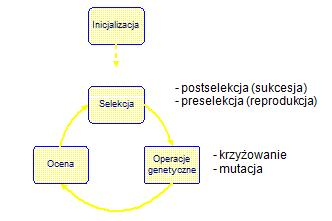
\includegraphics[width=.4\linewidth]{10/algo_ewolucyjne_schemat}
\caption*{Zadanie 10.4: Schemat algorytmów ewolucyjnych}
\end{figure}
}




% 5 - 162
\answer
{Do znalezienia minimalnego czasu wykonania przedsięwzięcia reprezentowanego poprzez graf (sieć) stosuje się metodę ścieżki krytycznej. Na czym polega ta metoda?}
{Na wyznaczeniu najdłuższej ścieżki prowadzącej z wierzchołka początkowego do wierzchołka końcowego.}
{T}
{}
{
Metoda ścieżki krytycznej polega na wyznaczeniu ścieżki w grafie zadań, dla której łączny czas trwania tych zadań jest największy. Czas ten jest minimalnym czasem trwania przedsięwzięcia.

\begin{enumerate}
\item{Najwcześniejszy termin zajścia zdarzenia $j$ oznaczamy przez $t_{j}^w$ i wyznaczamy ze wzoru:\\
$t_1^w = 0 $ : pierwsze zdarzenie może zajść najwcześniej w czasie 0 \\
$t_j^w = max\{t_i^w+t_{i,j}\}$ po $i$ należącym do zbioru wierzchołków, w których rozpoczynają się zadania dochodzące do wierzchołka $j$. $t_j^w$ jest długością najdłuższej ścieżki od wierzchołka 1 do $j$.\\
Czyli zaczynamy od pierwszego wierzchołka i tworzymy najdłuższą ścieżkę.\\
$t_1^w=0, t_2^w=5, t_3^w=10, t_4^w=12, t_s^w=20$}

\item{Najpóźniejszy termin zajścia zdarzenia $i$:\\
$t_s^p = t_s^w$ Ostatnie zdarzenie ma czas wyliczony w punkcie 1\\
$t_i^p = max \{i_j^p - t_{i,j}\}$ po $j$ należącym do zbioru zdarzeń, w których kończą się zadania rozpoczęte z wierzchołka $i$.

Zaczynamy w końcowym wierzchołku, który ma czas wyliczony jako najwcześniejszy termin zajścia zdarzenia w tym węźle, wracamy do wierzchołka startowego i wartość w każdym węźle wynosi (wartość poprzedniego - wartość w ścieżce). W przypadku większej ilości możliwości dojścia do węzła wybieramy tak, by ta wartość była największa. 

\underline{Przykład:} idąc od węzła s do 4 $t_s^p = 20$, $t_4^p = 12$, a z s do 3  $t_s^p = 20$, $t_3^p = 14$. Do węzła 2 możemy dojść przez 3 lub 4, jednak wartość w 2 będzie największa idąc przez 3, więc ten węzeł będzie w ścieżce.
$t_s^p=t_s^w=20, t_4^p=12, t_3^p=14, t_2^p=13, t_1^p=3$}

\begin{figure}[!ht]
\centering
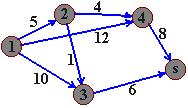
\includegraphics[width=0.5\textwidth]{10/cpm}
\caption*{Zadanie 10.5: Przykład}
\end{figure}

\end{enumerate}
}



% 6 - 163
\answer
{Dla której z podstawowych technik obliczeń ewolucyjnych charakterystyczna jest adaptacja zasięgu mutacji?}
{Dla strategii ewolucyjnych.}
{T}
{}
{ \\
Adaptację zasięgu mutacji stosujemy w strategiach ewolucyjnych, a konkretnie w strategiach $(\mu,\lambda)$ oraz $(\mu+\lambda)$. Strategie $(1+1)$ oraz $(1+\lambda)$ zasięg mutacji określany jest przez dobór odpowiednika współczynnika.
\vspace{0.1cm}

\noindent$\mu$ - populacja rodziców, 
$\lambda$ - populacja potomków
\vspace{0.4cm}

\noindent Inne techniki obliczeń ewolucyjnych:
\begin{itemize}
\item Algorytmy genetyczne
\item Programowanie genetyczne
\item Programowanie ewolucyjne
\item Algorytmy immunogenetyczne
\end{itemize}
}




% 7 - 164
\answer
{Dany jest pierwotny program liniowy postaci:
$c^T x \to max, A \cdot x \leq b, x \geq 0.$
Program dualny do niego ma postać:}
{$b^T y \to max, A^T \cdot y \leq b, y \geq 0.$}
{F}
{$b^T y \to min, A^T \cdot y \geq c, y \geq 0.$}
{
\begin{center}
\begin{tabular}{c | c}
Program pierwotny  & Program dualny       \\ 
\hline \hline
$c^Tx \to max$     & $b^T y \to min$      \\
$A \cdot x \leq b$ & $A^T \cdot y \geq c$ \\
$x \geq 0$         & $y \geq 0$           \\ 
\hline
$c^Tx \to min$     & $b^T y \to max$      \\
$A \cdot x \geq b$ & $A^T \cdot y \leq c$ \\
$x \leq 0$         & $y \leq 0$           \\
\end{tabular}
\end{center}

\begin{itemize}
\item $A$ -- macierz $M\times N$ współczynników stojących po lewej stronie układu warunków ograniczających (czyli mamy $M$ warunków ograniczających i $N$ zmiennych decyzyjnych)
\item $b$ -- wektor kolumnowy $M$ wyrazów wolnych układu warunków ograniczających 
\item $c^T$ -- wektor wierszowy $N$ współczynników funkcji celu
\item $x$ -- wektor kolumnowy $N$ zmiennych decyzyjnych zagadnienia pierwotnego
\item $y$ -- $M$-elementowy wektor kolumnowy nowych zmiennych decyzyjnych (zmiennych dualnych).
\end{itemize}

Program dualny do standardowego zagadnienia maksymalizacji jest standardowym zagadnieniem minimalizacji, zaś program dualny do standardowego zagadnienia minimalizacji jest standardowym zagadnieniem maksymalizacji (czyli jak maksymalizujemy program pierwotny to minimalizujemy program dualny, jak minimalizujemy program pierwotny to maksymalizujemy program dualny).

Charakterystyczne dla programu dualnego jest to, że ma tyle warunków ograniczających, ile zmiennych miał program pierwotny, zaś zmiennych ma tyle, ile warunków miał program pierwotny. Dalej, w programie dualnym wagami funkcji celu są wyrazy wolne zagadnienia pierwotnego, zaś wyrazami wolnymi są wagi funkcji celu programu pierwotnego. Te własności programu dualnego sprawiają, że może być atrakcyjny dla decydenta. Mianowicie, pierwotny problem decyzyjny może mieć liczne zmienne decyzyjne, ale niewielką liczbę warunków ograniczających, zatem program dualny będzie mieć liczne warunki ograniczające, ale niewielką liczbę zmiennych decyzyjnych, przez co może być łatwiejszy do rozwiązania. I gdy istnieje związek (przejście) między rozwiązaniami programów pierwotnego i dualnego, to korzyść z posiadania programu dualnego jest oczywista.
}




% 8 - 165
\answer
{Co nazywamy mostem grafu?}
{Minimalną liczbę krawędzi grafu, których usunięcie zmienia graf w niespójny lub trywialny.}
{F}
{\textbf{(Możliwe dwie)} 
\begin{enumerate}[label=(\alph*)]
\item \textbf{Krawędź grafu spójnego której usunięcie z grafu zmienia go w graf niespójny lub trywialny.}
\item \textbf{Krawędź, której usunięcie spowoduje wzrost liczby składowych spójności grafu.}
\end{enumerate}
}
{Patrz punkt \textbf{10.9}.}




% 9 - 166
\answer
{Jak nazywamy podzbiór $V' \subset V$ zbioru wierzchołków grafu $G = (V, E)$, taki, że każdy węzeł nienależący do $V'$ jest sąsiedni do pewnego elementu z $V'$?}
{Zbiór niezależny.}
{F}
{\textit{To wygląda na pytanie typu ,,odrzuć odpowiedzi, które na pewno nie są prawidłowe'' -- np. znasz pojęcie zbioru niezależnego i wiesz, że to nie to}}
{ 
\begin{itemize}
\item \textbf{Zbiór niezależny} -- zbiór takich wierzchołków w grafie, pomiędzy którymi nie ma żadnej krawędzi
\item \textbf{Podgraf} -- graf uzyskany poprzez usunięcie części wierzchołków wraz z kończącymi się w nich krawędziami
\item \textbf{Graf spójny} –- dla każdej pary wierzchołków istnieje ścieżka, która je łączy
\item \textbf{Graf niespójny} -- graf nieposiadający powyższej własności
\item \textbf{Graf trywialny} -- graf składający się tylko z jednego wierzchołka
\item \textbf{Spójna składowa grafu} -- taki podgraf, który można ,,wydzielić'' z całego grafu bez usuwania krawędzi; graf spójny ma jedną spójną składową
\item \textbf{Graf acykliczny} -- graf niezawierający drogi zamkniętej
\item \textbf{Drzewo} -- spójny, nieskierowany graf acykliczny
\item \textbf{Drzewo spinające grafu} -- spójny, acykliczny podgraf danego grafu, zawierający wszystkie wierzchołki
\item \textbf{Graf pełny} -- wszystkie wierzchołki są ze sobą bezpośrednio połączone
\item \textbf{Klika} -- podgraf pełny
\end{itemize}
}




% 10 - 167
\answer
{Jak nazywamy system obsługi zadań, w którym każde zadanie musi przejść przez wszystkie maszyny w jednakowym, ściśle określonym porządku?}
{System otwarty.}
{F}
{System przepływowy.}
{ \\
W przypadku maszyn dedykowanych rozróżniane są następujące systemy obsługi zadań:
\begin{itemize}
\item \textbf{przepływowy (flow-shop)} -- każde zadanie musi przejść przez wszystkie maszyny w ściśle określonym porządku (każde zadanie składa się zatem z $m$ operacji)
\item \textbf{ogólny / gniazdowy (job-shop)} -- kolejność maszyn mających wykonać operacje jest różna, ale ściśle określona dla każdego zadania (zadania mogą mieć różną ilość operacji)
\item \textbf{otwarty (open-shop)} -- w systemie otwartym wytworzenie każdego wyrobu wymaga operacji na wszystkich maszynach, ale kolejność ich wykonywania jest dowolna i nieustalona.
\end{itemize}
}




% 11 - 168
\answer
{W algorytmie symulowanego wyżarzania z sąsiedztwa bieżącego rozwiązania bazowego losuje się jedno rozwiązanie. Co się dzieje, jeżeli jest ono gorsze od dotychczasowego rozwiązania bazowego?}
{Zastępuje bieżące rozwiązanie bazowe, jeżeli parametr zwany temperaturą jest mniejszy od zera.}
{F}
{Znalezione rozwiązanie zastępuje poprzednie z pewnym prawdopodobieństwem zależnym m.in. od współczynnika nazywanego temperaturą. Temperatura zmniejsza się wraz z kolejnymi iteracjami, co pociąga za sobą spadek prawdopodobieństwa wybrania gorszego rozwiązania.}
{ \\
Termin wyżarzanie pochodzi z metalurgii i dotyczy termodynamicznego procesu studzenia. Jeżeli płynna stal jest schładzana wystarczająco wolno, to ma tendencję do krzepnięcia w strukturze o minimalnej energii. Metoda symulowanego wyżarzania opiera się na analogii do tego procesu. Jej celem jest wyprowadzenie trajektorii poszukiwań z ekstremum lokalnego lub uniknięcie takiego ekstremum. W metodzie tej, z sąsiedztwa aktualnego rozwiązania nie jest wyszukiwane najlepsze rozwiązanie, tylko wybiera się rozwiązanie w sposób losowy. Jeżeli to wylosowane rozwiązanie jest lepsze od bieżącego, to staje się ono nowym rozwiązaniem. W przeciwnym przypadku znalezione rozwiązanie zastępuje poprzednie z pewnym prawdopodobieństwem zależnym m.in. od temperatury. 

Temperatura jest zmieniana w czasie iteracji według tzw. schematu chłodzenia. Im wyższa, tym prawdopodobieństwo wyboru gorszego rozwiązania jest większe. Im niższa, tym algorytm jest bardziej zbliżony w działaniu do typowych metod iteracyjnych. To właśnie znajduje odzwierciedlenie w drugim ważnym aspekcie algorytmu symulowanego wyżarzania czyli w powolnym ochładzaniu.

Na początku działania algorytmu temperatura jest wysoka, dzięki czemu algorytm może bardzo często zmieniać konfigurację rozwiązania, niejednokrotnie wybierając rozwiązanie gorsze. Wraz z kolejnymi iteracjami algorytmu temperatura spada i wybierane są częściej rozwiązania lepsze. Pod koniec pracy algorytmu, temperatura jest na tyle niska, że prawdopodobieństwo wyboru gorszego rozwiązania jest bliskie zeru. Algorytm zachowuje się wówczas, jak typowy algorytm iteracyjny i stara się maksymalnie ulepszyć rozwiązanie.
}




% 12 - 169
\answer
{W teorii złożoności wszystkie problemy decyzyjne, które w wielomianowym czasie rozwiązuje niedeterministyczna maszyna Turinga, tworzą pewną klasę problemów. Jak brzmi jej nazwa?}
{Klasa NP.}
{T}
{}
{ \\
\textbf{Klasa P} --  wszystkie problemy decyzyjne, które w co najwyżej wielomianowym czasie rozwiązuje deterministyczna maszyna Turinga

\textbf{Klasa NP} -- wszystkie problemy decyzyjne, które w co najwyżej wielomianowym czasie rozwiązuje niedeterministyczna maszyna Turinga 

P $\subset$ NP 

Mówimy, że problem decyzyjny $\Pi_1$ jest NP-zupełny, jeśli $\Pi_1 \in$ NP i dla każdego innego problemu decyzyjnego $\Pi_2$  NP zachodzi: $\Pi_2$  $\Pi_1$.

Dla wykazania trudności rozważanego problemu \underline{optymalizacyjnego} (tzn. problemu w którym należy ekstremalizować pewną funkcję celu) wystarcza wykazanie NP-zupełności odpowiadającego mu problemu \underline{decyzyjnego} (tzn. problemu na który odpowiadamy tak lub nie). Mówimy wtedy, że dany problem optymalizacyjny jest \textbf{NP-trudny}.
}





% 13 - 170
\answer
{Zastosowanie metody programu dualnego pozwala na:}
{Zamianę problemu optymalizacyjnego na równoważny -- decyzyjny.}
{F}
{Zamianę problemu pierwotnego -- który posiada liczne zmienne decyzyjne, ale niewielką liczbę warunków ograniczających -- na program dualny, który będzie mieć liczne warunki ograniczające, ale niewielką liczbę zmiennych decyzyjnych, przez co może być łatwiejszy do rozwiązania.
}
{ Patrz punkt \textbf{10.7}.
}




% 14 - 171
\answer
{Dane są algorytmy A i B o złożonościach odpowiednio $O_A(n^3)$ i $O_B((\log n)^3)$. Oba algorytmy wywołano dla pewnych danych wejściowych: $a$ (dla A) i $b$ (dla B). Szybciej (w sensie czasu mierzonego w sekundach) wykona się algorytm:}
{B}
{T}
{}
{Algorytm B ma złożoność logarytmiczną.

\begin{figure}[!ht]
\centering
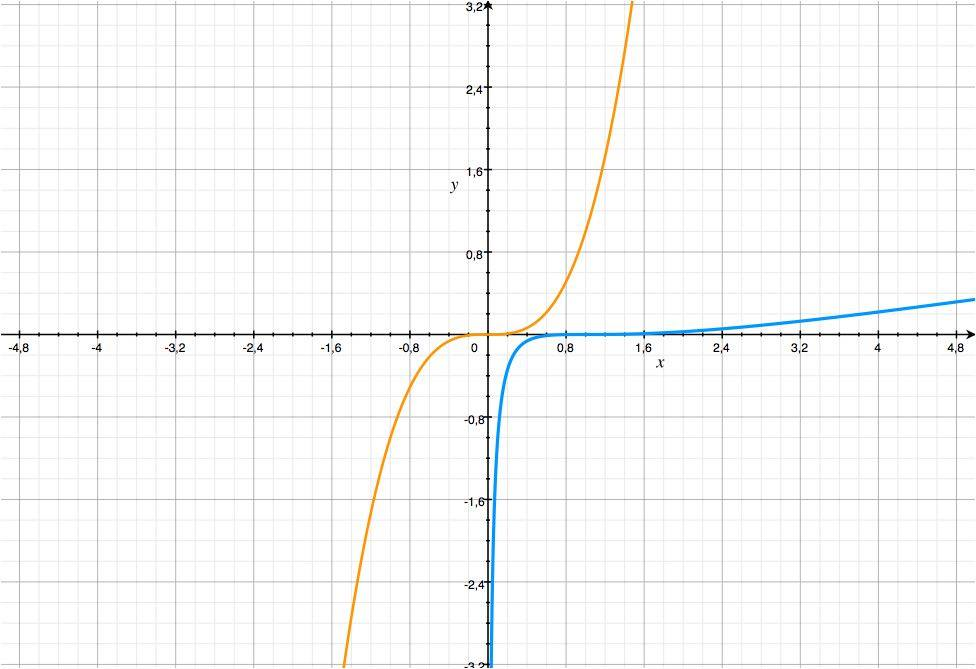
\includegraphics[width=\textwidth]{10/10-4-2}
\caption*{Zadanie 10.14: Oś X to rozmiar danych wejściowych, oś Y to czas obliczeń. Mamy dodatkowo założenie, że X > 1. Widać, że wykresy się ładnie rozmijają i niezależnie od rozmiaru danych wejściowych czas obliczeń jest zawsze mniejszy dla złożoności $(\log x)^3$. Jeżeli wykresy by się przecinały, to znaczy że można znaleźć taki rozmiar danych wejściowych $a$ i $b$.}
\end{figure}
}




% 15 - 172
\answer
{W jakim celu w algorytmach ewolucyjnych stosuje się funkcję kary?}
{Zmniejszenia liczby osobników w populacji.}
{F}
{Funkcję kary stosuje się przy osobnikach reprezentujących niedopuszczalne rozwiązanie. Spowoduje ona dużo mniejsze prawdopodobieństwo przejścia selekcji przez danego osobnika. W zależności od tego, czy funkcję dopasowania minimalizujemy czy maksymalizujemy, wartość funkcji błędu należy do niej dodać bądź odjąć.}
{}

\chapter{Sieci komputerowe}
\PartialToc
%\startcontents[chapters]
%\printcontents[chapters]{}{1}{\section*{\contentsname}}
\answer
{Adres typu broadcast (rozgłoszenia) IP w wersji 4 dla sieci IP, w której
znajduje się host 110.104.1.10 i która okresla maska 255.0.0.0, to}
{110.104.1.0}
{F} %należy wpisać "T" (prawda™) lub "F" (FAŁSZ) 
{110.255.255.255}
{Adresy broadcast dla IP wersji 4 to adres który w danej sieci bajtowo zapisujemy jako ciąg 1. 
Dla IP 110.104.1.10 o masce 255.0.0.0 adres sieci to 110.0.0.0 (wszystkie bajty w pierwszym członie adresu zostały zachowane (255 w masce). Oznacza to, iż w 3 kolejnych członach zapisanych bajtowo znajdą się same 1). Jako iż każdy człon składa się z 8 bajtów adres ten zapisany w systemie dziesiętnym będzie miał wartość 110.255.255.255 }

\answer
{Pole o nazwie Time to Live w datagramie IP, które zabezpiecza przed zapętleniem rutowania datagramu pomiędzy kolejnymi ruterami w sieci zawiera:}
{Liczbę ruterów przez jakie datagram IP może zostać przekazany dalej }
{T} %należy wpisać "T" (prawda™) lub "F" (FAŁSZ) 
{Liczbę ruterów przez jakie datagram IP może zostać przekazany dalej }
{W przypadku czasu życia pakietów danych w sieci komputerowej jest to zwykle liczba przeskoków, które może on wykonać na swojej trasie. Każdy kolejny router IP na trasie danego pakietu zmniejsza wartość jego pola TTL o jeden. Jeśli router otrzyma pakiet z TTL równym 1, zmniejsza go do 0, odrzuca go i usuwa z sieci, a nadawca otrzyma komunikat ICMP o błędzie. Czas życia pakietu pomaga unikać przeciążenia sieci w przypadku źle skonfigurowanych tras routingu w routerach, np. występowania pętli w sieci.}

\answer
{Nazwa ramki stosowanej w technologii IEEE 802.11 i emitowanej przez
urządzenie Access Point i stosowanej między innymi w celu propagowania informacji o sieci bezprzewodowej,
to}
{Checker}
{F} %należy wpisać "T" (prawda™) lub "F" (FAŁSZ) 
{Beacon frame }
{Beacon frame to jedna z tzw. Management frames w standardzie IEEE 802.11. Zawiera informacje o sieci. Ramki te wysyłąne są z Access Pointów co jakiś czas i rozgłaszają obecność sieci.}

\answer
{Protokół UDP definiuje identyfikatory przesyłanych do hosta-odbiorcy datagramów
zwane numerami portów, o długosci}
{32}
{T lub F (patrz wyjąśnienie)} %należy wpisać "T" (prawda™) lub "F" (FAŁSZ) 
{32 lub 16 }
{Nagłówek UDP rozpoczynają 2 pola Port nadawcy oraz port odbiorcy. Każdy po 16 bitów. Ich łączna długość to 32.

UDP jeden z protokołów internetowych. UDP stosowany jest w warstwie transportowej modelu OSI.

Jest to protokół bezpołączeniowy, więc nie ma narzutu na nawiązywanie połączenia i śledzenie sesji (w przeciwieństwie do TCP). Nie ma też mechanizmów kontroli przepływu i retransmisji. Korzyścią płynącą z takiego uproszczenia budowy jest większa szybkość transmisji danych i brak dodatkowych zadań, którymi musi zajmować się host posługujący się tym protokołem. Z tych względów UDP jest często używany w takich zastosowaniach jak wideokonferencje, strumienie dźwięku w Internecie i gry sieciowe, gdzie dane muszą być przesyłane możliwie szybko, a poprawianiem błędów zajmują się inne warstwy modelu OSI. Przykładem może być VoIP lub protokół DNS.
}

\answer
{Wartosci adresu IPv6 oraz maski, określające wszystkie hosty w Internecie, to}
{ ::/0}
{F} %należy wpisać "T" (prawda™) lub "F" (FAŁSZ) 
{2000::/3 ???}
{Prawdopodobnie chodzi tutaj o Global Unicast - w IPv4 jest to publiczny adres IP, czyli taki który jest rutowany w całym internecie.}


\answer
{Istnienie zasady “Longest prefix match“ w rutowaniu IP spowoduje, że adres docelowy 200.200.200.1 datagtramu IP przy istnieniu w tablicy rutowania jednoczesnie reguł o wzorcach i maskach (podano w notacji CIDR): 200.200.200.0/18, 200.200.200.0/20, 200.200.200.0/22, 200.200.200.0/24
zostanie dopasowany do:}
{200.200.200.0/20}
{F} %należy wpisać "T" (prawda™) lub "F" (FAŁSZ) 
{200.200.200.0/24}
{Longest Prefix Match to algorytm stosowany przez rutery przy wyborze kolejnego rutera z tablicy rutowania. Jako, iż wiele wpisów w owej tablicy może pasować do jednego adresu. (w powyższym przykładzie wszystkie 4 pasują do podanego) to wybierane jest wejście z najdłuższą pasującą maską podsieci (w tym wypadku o długości 24).}


\answer
{Maksymalna długość pakietu IP wersja 4, licząc w bajtach, to}
{1024}
{F} %należy wpisać "T" (prawda™) lub "F" (FAŁSZ) 
{65,535}
{Długość ta wynosi tyle ponieważ w nagłówku pakietu IP znajduje się pole TOTAL LENGTH (oznaczające długość całego pakietu w bajtach). Pole to zajmuje 2 bajty (16 bitów). Oznacza to iż maksymalna liczba jaką można tam zapisać to binarnie $ 2 ^ 16 -1 $ czyli 65535 }


\answer
{Okreslenie stosowane wobec rutera MPLS (MultiProtocol Label Switching), będącego w danej sytuacji odbiorcą datagramów z etykietami MPLS od innego (nie będącego przedmiotem rozwazań to:}
{ Designated router}
{F} %należy wpisać "T" (prawda™) lub "F" (FAŁSZ) 
{Label switch router ? a nie chodzi tu o Downstream Router czyli według wykładów - dla datagramów - ten który odbiera datagramy MPLS ????}
{MPLS to technika stosowana przez routery, w której trasowanie pakietów zostało zastąpione przez tzw. przełączanie etykiet.

Na brzegu sieci z protokołem MPLS do pakietu dołączana jest dodatkowa informacja zwana etykietą (ang. Label). Router po odebraniu pakietu z etykietą (jest to z punktu widzenia danego routera etykieta wejściowa) używa jej jako indeksu do wewnętrznej tablicy etykiet, w której znajduje się następny punkt sieciowy (ang. next hop) oraz nowa etykieta (etykieta wyjściowa). Etykieta wejściowa jest zastępowana wyjściową i pakiet jest wysyłany do następnego punktu sieciowego (np. do następnego routera). Jeżeli następny router nie obsługuje protokołu MPLS, etykieta jest usuwana.

Przypisanie pakietowi etykiety na brzegu sieci odbywa się w tzw. procesie klasyfikacji. Pakiety, które będą w jednakowy sposób routowane przez sieć MPLS, klasyfikowane są do jednej klasy FEC (ang. Forwarding Equivalence Class) i otrzymują tę samą etykietę. Przykładowo, klasy FEC mogą być budowane na bazie adresów docelowych IP w nagłówku pakietu w taki sposób, że każda klasa FEC pokrywa się z pojedynczym wpisem w tablicy trasowania routera.

Przyporządkowanie danej klasy FEC do etykiety jest sygnalizowane innym routerom za pomocą protokołu dystrybucji etykiet. Pozwala to routerom na zbudowanie tablic etykiet. W zależności od konkretnego zastosowania, jako protokół do dystrybucji etykiet używany jest LDP, albo odpowiednio rozszerzone protokoły: RSVP lub BGP.}

\answer
{Ruter iBGP (internal Border Gateway Protocol), którego wprowadzenie~do systemu rutowania iBGP umożliwia znaczne zredukowanie ilości otwartych sesji BGP pomiędzy innymi ruterami (rezygnację~z tzw. Full-mesh) nosi nazwę:}
{Route Reflector}
{T}
{Route Reflector}
{RR - Route Reflector - Dzieli obszary działania na części - radykalnie zmniejszając liczbę sesji pomiędzy ruterami iBGP. W jednym AS(Systemie autonomicznym) może występować wiele RR. Przekazuje od komunikaty od klientów RR do innych routerów iBGP.}

\answer
{Liczba klas CoS (Class~of Service), definiowanych przez podstawowy mechanizm implementacji QoS (Quality~of Service)~w Ethernet (czyli standard IEEE 802.1p),~to:}
{16}
{F}
{8}
{Class of Service - jest formą priorytetowego kolejkowania, która jest używana w protokołach sieciowych. W Ethernet przyjmuje wartości od 0 do 7.}

\answer
{Wariant protokołu STP (Spanning Tree Protocol, IEEE 802.1d) pozwalający~w technologii Ethernet~na logiczne grupowanie sieci VLAN (Virtual LAN)~i budowanie mniejszej liczby drzew rozpinających (po jednym Spanning Tree dla każdej zdefiniowanej grupy),!to:}
{PVSTP (Per VLAN Spanning Tree Protocol)}
{F}
{MSTP - Multiple Spanning Tree Protocol}
{Nie ma tu zbyt wiele do wyjaśniania}

\answer
{Rodzaje (grupy) urządzeń fizycznych definiowanych~w technologii ZigBee,~to:}
{ZigBee End Device, ZigBee Coordinator, ZigBee Router}
{T}
{ZigBee End Device, ZigBee Coordinator, ZigBee Router}
{ZED - ZigBee End Device - urządzenie czujnika, sterownika lub inne, które jest faktycznym źródłem lub odbiorcą danych.
ZC - ZigBee Coordinator - pełni rolę urządzenia zarządzającego parametrami transmisji, jest centralnym węzłem sieci (do niego podłączone są inne urząddzenia), może być mostkiem do innych sieci.
ZR - ZigBee Router - komunikuje inne urządzenia ZigBee, służy głównie do przedłużania zasięgu, lecz także komunikuje się~z innymi technologiami (network level).}

\answer
{Nazwa procesu przekazywania wiedzy o trasach pomiędzy różnymi protokołami rutowania dynamicznego IP w ruterach IP,~to:}
{Redystrybucja}
{T}
{Redystrybucja}
{Redystrybucja (protokołu) - zabieg przekazywania informacji o trasach pozyskanych z użyciem jednego  z obsługiwanych i działających protokołów rutowania.}

\answer
{Symbole literowe, określające rodzaje popularnych~w sieciach komputerowych wtyków światłowodowych,~to:}
{LC, SC, MTRJ}
{T}
{LC, SC, MTRJ}
{LC - najbardziej popularne złącze światłowodowe - simplex/duplex.
SC - poprawiona polaryzacja, większa stabilnośc mechaniczna łącza w porównaniu do simplex-ST.
MTRJ - ostatnio bardzo popularyzowane (tylko duplex)}

\answer
{Co określa standard IEEE 802.1Q?}
{Wirtualne sieci LAN (VLAN) budowane~w środowisku transportującym ramki}
{T}
{Wirtualne sieci LAN (VLAN) budowane~w środowisku transportującym ramki}
{Standard ten opisuje działanie wirtualnych sieci LAN (VLAN) budowanych w środowisku transportującym ramki}

\answer
{Protokół umożliwiający konwersję adresu IP zdalnej stacji~na jej adres MAC~w Ethernet,~to:}
{MLD (Multicast Listener Discovery)}
{F}
{ARP}
{ARP - Address Resolution Protocol -  protokół sieciowy umożliwiający mapowanie logicznych adresów warstwy sieciowej (warstwa 3 - IP) na fizyczne adresy warstwy łącza danych (2 - MAC).}

\answer
{Co zawiera pole Extended Unique Identifier (EUI) w adresie IPv6?}
{Adres IP w wersji 4 przypisany do stacji}
{F}
{Zawiera adres MAC urządzenia uzupełniony pośrodku o wartość: 0xFFFE}
{EUI - Extended Unique Identifier - adres MAC (48 bitów) zostaje uzupełniony pośrodku wartością 0xFFFE np. adres MAC - 00:0C:29:0C:47:D5, uzupełniony - 00:0C:29:FF:FE:0C:47:D5.}

\answer
{Domyślna wartość metryki Administrative Distance~w tablicy rutowania IP ruterów (np. Cisco, Juniper, Helwet Packard) przewidziana dla protokołu RIP (Routing Information Protocol),~to:}
{110}
{F}
{120}
{Tak zostało z góry ustalone.}

\answer
{W technologii Fibre Channel (stotowanej w sieciach SAN) port przełącznika Switch Fabric mogący pracować w topologii pętli arbitrażowej (pętli~z arbitrażem) sieci Fibre Channel, to port typu:}
{FL}
{T???????}
{FL}
{FL - Fabric-Loop Port, FL\_Port - port przełącznika mogący pracować~w topologii sieci arbitrażowej, używany do podłączenia portów NL do przełącznika.}

\answer
{Dwie pod-warstwy definiowane~w ramach warstwy drugiej modelu ISO-OSI to odpowiednio:}
{LAN i WAN}
{F}
{LLC i MAC}
{LLC - Logical Link Control, MAC - Media Access Control)}

\answer
{Zadaną~w jednostce dBm efektywną moc wypromieniowaną (Effective Isotropic Radiated Power, EIRP) bezprzewodowego urządzenia nadawczego stosowanego~w technologii sieciowej~na podstawie mocy wypromieniowanej P zadanej w watach można obliczyć stosujżc wzór:}
{EIRP = 1 / (P*1mW)}
{F}
{$EIRP = 10*log_{10}(\frac{P}{1mW})$}
{P - moc wypromieniowana}

\answer
{Jednostka wysokości urządzenia sieciowego montowanego~w standardzie RACK wynosząca 1,75 cala (44,45 mm) oznaczana jest symbolem:}
{h}
{F}
{U}
{U - najmniejsza możliwa wysokość urządzenia 1U = 1.75cala = 44.45mm}

\answer
{Rodzaj obszaru (area)~w domenie OSPF (Open Shortest Path First) nie otrzymującego żadnych informacji~o zewnętrznych (external) trasach rutowania OSPF,~to:}
{backbone}
{F}
{Stub area}
{Stub area - obszar wyizolowany - otrzymuje jedynie wyjście na zewnątrz, nie otrzymuje i nie wysyła informacji o sieciach.}

\answer
{Parametr~o nazwie "Wielkość okna"(Window size), którego wartość przekazywana jest~w datagramach potwierdzenia TCP (Transmission Control Protocol Acknowledgment)~w kierunku od odbiorcy do nadawcy ma na celu:}
{Określić ilość danych, jaką nadawca może~w danej chwili wysłać (służy do sterowania przepływem)}
{T?????? - w dobrą stronę ja myślę, bo już mi się miesza :/}
{Określić ilość danych, jaką nadawca może~w danej chwili wysłać (służy do sterowania przepływem)}
{Rozmiar okna - 16-bitowe pole używane przez komputer docelowy w celu poinformowania komputera źródłowego o tym, ile danych jest gotów przyjąć~w jednym segmencie TCP.}

\answer
{Dwa rodzaje obszarów (area)~w protokole rutowania dynamicznego IS-IS (Intermediate System to Intermediate System), to:}
{LAN i WAN}
{F}
{Level 1, Level 2}
{Level 1 - intra-area - traktowany jako backbone szkieletu sieci objętej protokołem, routery Level 1 komunikują się tylko z routerami Level 1.
Level 2 - inter-area - routery Level 2 komunikują się tylko z routerami Level 2.}


\chapter{Paradygmaty programowania}
\lstloadlanguages{Prolog}
\lstset{language=Prolog}

% 198
\section{IT1A\_W05}
\textbf{Podstawowym, deklaratywnym językiem programowania logicznego jest?}
\vspace{0.4cm}
Odpowiedź: \newline
Do grupy deklaratywnych języków programowania logicznego zaliczamy:
\begin{itemize}
\item SQL
\item \textsc{Prolog}
\end{itemize}
\vspace{0.4cm}
Żródło: \url{http://ai.ia.agh.edu.pl/wiki/_media/pl:dydaktyka:miw:2011:jezyki_paradygmaty_v1_1.pdf}

% 199
\section{IT1A\_W05}
\textbf{Które z poniższych mechanizmów są wbudowane w interpreterze języka \textsc{Prolog}?}
Odpowiedź: \newline
Prolog udostępnia mechanizmy:
\begin{itemize}
\item  rekurencji -- jak metody przetwarzania informacji,
\item unifikacji -- mechanizmy dopasowywania wzorców,
\item rezolucji -- metody wnioskowania logicznego,
\end{itemize}
Źródło:
\url{http://ai.ia.agh.edu.pl/wiki/pl:prolog:prolog_lab:wprowadzenie\#programowanie_nieklasyczne}



%200
\section{IT1A\_W05}

\textbf{Rozważmy następującą definicję predykatu \lstinline!member/2!:}
\begin{lstlisting}[language=Prolog, frame=trbl]
member(H,[H|T]).
member(H,[_|T]):- member(H,T).
\end{lstlisting}
Dla wywołania \lstinline!member(X,[0,1,[2,3],4])! interpreter zwróci:

Odpowiedź: \newline
X = 0 ; \newline
X = 1 ; \newline
X = [2, 3] ; \newline
X = 4 ; \newline
false. \newline


%201
\section{IT1A\_W05}
Rozważmy następującą definicję predykatu \lstinline!member/2!:
\begin{lstlisting}[language=Prolog, frame=trbl]
member(H,[H|T]).
member(H,[_|T]):- member(H,T).
\end{lstlisting}
Dla wywołania \lstinline!member(X,[0,1,2,1,3,1,4])! interpreter zwróci:

Przykładowa ODP: 5 rozwiązań (nie powtórzy rozwiązania \lstinline!X = 1! - fałsz

Poprawna odpowiedź

X = 0 ; \newline
X = 1 ; \newline
X = 2 ; \newline
X = 1 ; \newline
X = 3 ; \newline
X = 1 ; \newline
X = 4 ; \newline
false. \newline


%202
\section{IT1A\_W05}

\textbf{Rozważmy następującą definicję predykatu \lstinline!append/2!: do łączenia list}
\begin{lstlisting}[language=Prolog, frame=trbl]
appendd([],L,L).
appendd([H|T],L,[H|TL]):- appendd(T,L,TL).
\end{lstlisting}
\textbf{Dla wywołania \lstinline!append(L1,L2,[1,2,3,4,5])! interpreter zwróci:}
\vspace{0.4cm}

Odpowiedź: \newline
L1 = [], 			\newline
L2 = [1, 2, 3, 4, 5]\newline
false				\newline

%203
\section{IT1A\_W05}

\textbf{Rozważmy następującą definicję predykatu \lstinline!append/3! do łączenia list:}
\begin{lstlisting}[language=prolog, frame=trbl]
append([],L,L).
append([H|T],L,[H|TL]):- append(T,L,TL).
\end{lstlisting}

\vspace{0.4cm}
Odpowiedź: \lstinline!append(_,[E],L).!

%204
\section{IT1A\_W05}

\textbf{Rozważmy następujący program w \textsc{Prolog}}
\begin{lstlisting}[language=Prolog, frame=trbl]

p(a).
p(b).
p(c).
p(a).
p(c).

run :- 
	p(X),
	assert(q(X)),
	fail.
	
\end{lstlisting}
\textbf{Po skompilowaniu i wykonaniu programu z wywołaniem \lstinline!run!:}
\vspace{0.4cm}

Odpowiedź: \newline
W pamięci zostanie zapisane 5 faktów, [q(a),q(b),q(c),q(a),q(c)])
false.

\vspace{0.4cm}
Żródło: \url{http://alumni.cs.ucr.edu/~vladimir/cs171/prolog_2.pdf} \newline
Źródło: \url{http://boklm.eu/prolog/page_5.html} \newline


%205
\section{IT1A\_W05}

\textbf{Rozważmy następujący program w \textsc{Prologu}:}
\begin{lstlisting}[language=prolog, frame=trbl]
ln(0,[]) :- !.
ln(N,[N|L]):- N1 is N-1, ln(N1,L).
\end{lstlisting}
\textbf{Po skompilowaniu i wykonaniu programu z wywołaniem \lstinline!ln(7,L)!:}

\vspace{0.4cm}
Odpowiedź:\newline
Dostaniemy listę: \lstinline!L = [7, 6, 5, 4, 3, 2, 1].!


%206
\section{IT1A\_W05}

\textbf{Rozważmy następujący program w \textsc{Prolog}}
\begin{lstlisting}[language=Prolog, frame=trbl]

s1(X) :- not(p(X)),!,q(X).
s2(X):- q(X), not(p(X)).
p(a).
q(b).
	
\end{lstlisting}
\textbf{Po skompilowaniu i wykonaniu programu:}
\vspace{0.4cm}
Odpowiedź: \newline
s1(X). \newline
false. \newline
		\newline
s2(X).  \newline
X = b.  \newline

\vspace{0.4cm}
Źródło: \url{http://boklm.eu/prolog/page_5.html} \newline


%207
\section{IT1A\_W05}

\textbf{Rozważmy następujące propozycje programów iteracyjnego sumowania elementów zadanej listy w \textsc{Prologu}:}
\textit{Tutaj miałyby być te programy...}

\vspace{0.4cm}
Przykładowa odpowiedź: \newline
"Zaden, w \textsc{Prologu} nie da się implementować obliczeń iteracyjnych"

Moja odpowiedź:\newline
Domyślam się że poprawną odpowiedzią mogłoby być:
\begin{lstlisting}[language=prolog, frame=trbl]
sumList(L,S):- sumList(L,0,S).
sumList([H|T],SS,S):-
	SS1 is SS + H,
	sumList(T,SS1,S).
sumList([],SS,S):-
	!,
    S is SS.
\end{lstlisting}
To prawda, że w Prologu nie ma czegoś takiego, jak pętla i tradycyjna iteracja, ale można ją niejako osiągnąć przez umieszczanie wywołań rekurencyjnych jako ostatniej instrukcji w funkcji. 

Przydałaby się weryfikacja jakiegoś prolog mastera.

%208
\section{IT1A\_W05} 
\textbf{Jaki typ w Haskellu będzie miało następujące wyrazenie: r x = x: r x}

\vspace{0.4cm}
Przykładowa odpowiedź: r :: Integer a => a -> [a] \newline
Odpowiedź: r :: a -> [a] \newline
Wyjaśnienie: Wyrażenie to przyjmuje obiekt i zwraca liste, jednak nie jest ograniczone do typu Integer (typ jest zależny od x)

%209
\section{IT1A\_W05} 
\textbf{Jak wygląda poprawna wartość dla typu data Tree a = L a | N (Tree a) a (Tree a)}

\vspace{0.4cm}
Przykładowa odpowiedź: N (L 4) 5 (L ’4’) \newline
Odpowiedź: N (L 4) 5 (L 4) lub N (L '4') '5' (L ’4’) \newline
Wyjaśnienie: 'a' musi być wszędzie tego samego typu, nie może być raz integer (4) a potem char('4') 

%210
\section{IT1A\_W05} 
\textbf{Haskell jest językiem opartym o paradygmat:}

\vspace{0.4cm}
Odpowiedź: Funkcyjny

%211
\section{IT1A\_W05} 
\textbf{Mechanizm typów w języku Haskell}
Odpowiedź: Silny, statyczny.\newline
Wyjaśnienie:\newline
Rodzaje ze względu na siłę:
\begin{itemize}
\item silne - każde wyrażenie ma ustalony typ, nie można go używać w kontekście innych typów,
\item słabe - typ może być zmieniony automatycznie, jeśli kontekst tego wymaga
\end{itemize}

Ze względu na czas przypisywania typów do zmiennych:
\begin{itemize}
\item dynamiczne - przypisywanie typów do wartości przechowywanych w zmiennych w czasie wykonywania programu,
\item statyczne - nadawanie typów zmiennym w czasie kompilacji programu
\end{itemize}

Haskell ma mechanizm zwany type inference - wnioskuje typy na podstawie wartości:
\begin{lstlisting}
:t 'a' 
'a' :: Char 
\end{lstlisting}
Funkcje także mają typ:
\begin{lstlisting}
addThree x y z = x + y + z
addThree :: Int -> Int -> Int -> Int
\end{lstlisting}

%212
\section{IT1A\_W05} 
\textbf{Zaznacz prawdziwe zdania: (opcja A podana, reszta wymyślone)
\begin{itemize}
\item A. W programowaniu funkcyjnym koncepcja funkcji jest taka jak w algebrze.
\item B. Programowanie funkcyjne opiera się na rachunku Lambda.
\item C. Dobrym nawykiem w programowaniu funkcyjnym jest, aby zmienne były immutable.
\item D. W programowaniu funkcyjnym możemy korzystać jedynie z wbudowanych typów danych.
\end{itemize}
}
Odpowiedź: A, B, C 

%213
\section{IT1A\_W05} 
\textbf{Funkcje wyższego rzędu w programowaniu funkcyjnym}\newline
Odpowiedź: \newline
To funkcje, które przyjmują inne funkcje jako parametry lub zwracają inne funkcje jako rezultat.\newline
Wyjaśnienie:
Ideą programowania funkcyjnego jest używanie funkcji jak każdej innej wartości. Skutek jest taki, że dopuszczone jest przyjmowanie funkcji jako parametry lub ich zwracanie. Przykładem jest funkcja map, która przyjmuje funkcję przekształcającą elementy listy.

%214
\section{IT1A\_W05} 
\textbf{Jaki mechanizm w językach funkcyjnych pozwala na wykonanie operacji na zbiorze danych?} \newline
Odpowiedź: Rekurencja, funkcje specyficzne dla języka.\newline
Wyjaśnienie:\newline
Rozumiejąc ‘operacje na zbiorze danych’ jako przechodzenie / modyfikowanie zbioru, możemy wyróżnić dwa sposoby - implementacja operacji za pomocą rekurencji oraz używanie funkcji wbudowanych w język (np. fold, map, niektóre języki zorientowane funkcyjnie mają pętle).

%215
\section{IT1A\_W05} 
\textbf{Zaznacz prawdziwe zdania dotyczące programowania funkcyjnego (opcja A podana, reszta wymyślone) :}
\begin{itemize}
\item A. Niektóre języki imperatywne zostały wyposazone w konstrukcje z jezyków funkcyjnych.
\item B. Wszystkie języki funkcyjne są skonstruowane w oparciu o logical programming.
\item C. Programowanie funkcyjne może być połączone z programowaniem obiektowym.
\item D. Koncepcja programowania funkcyjnego opiera się o implementacje funkcji, które nie mają skutków ubocznych.
\end{itemize}

Odpowiedź: A, C, D \newline
Wyjaśnienie:
A - na przykład Stream API w Javie 8,
B - Prolog jest oparty o logical programming, Haskell już nie
C - np. konstrukcje Haskella, Scali
D - skutki uboczne są dopuszczone w wielu językach funkcyjnych, ale dobrym nawykiem jest ich unikanie.


\setcounter{chapter}{12}
\chapter{Programowanie miktrokontrolerów i mikroprocesorów}
\PartialToc
%\startcontents[chapters]
%\printcontents[chapters]{}{1}{\section*{\contentsname}}
\setcounter{section}{215}

%-----------------
\answer
{Ile rejestrów 8-bitowych dostępnych dla programisty znajduje się w procesorach z rodziny x86?}
{6}
{F}
{8}
{
	Innej poprawnej nie ma. Rysunek poniżej
	\begin{center}
		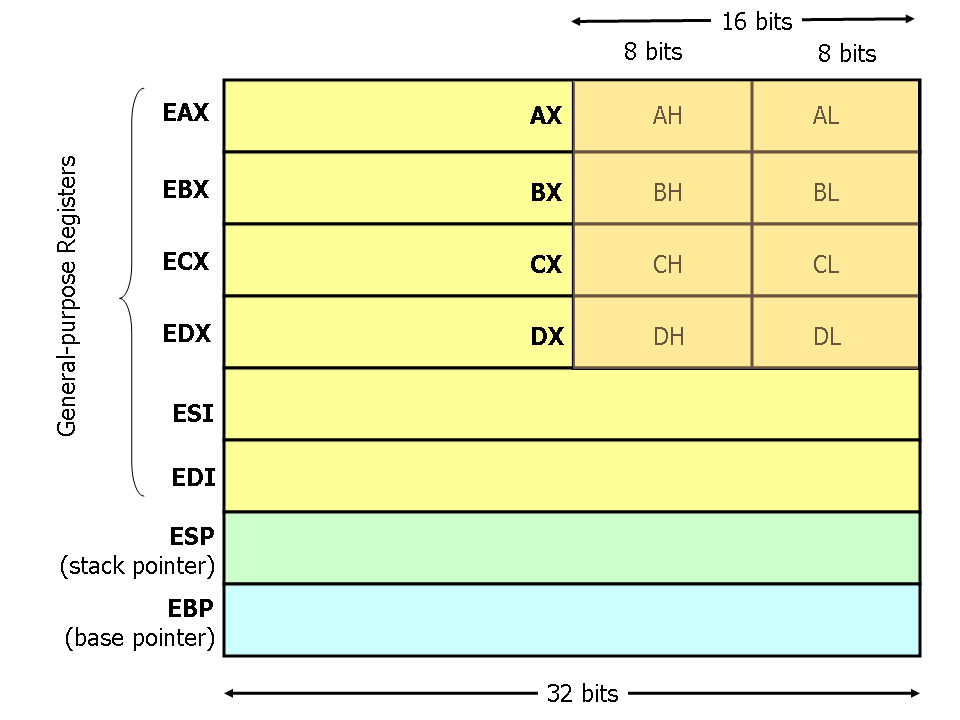
\includegraphics[width=6cm]{13/img/x86-registers.png}
		\captionof{figure}{Struktura rejestrów procka x86}
	\end{center}
}
%-----------------
\answer
{Jaki tryb adresowania wykorzystuje rozkaz ADDL (\%ebx),\%eax?\\}
{bezposredni}
{F}
{pośredni}
{
	Główny podział:
	\begin{itemize}
		\item bezpośredni (ang. direct)
		\item pośredni (ang. indirect)
	\end{itemize}
	Bardziej szczegółowo:
	\begin{itemize}
		\item rejestrowy (ang. register)
		\item rejestrowy pośredni (ang. register indirect)
		\item z przesunieciem (indeksowanie) (ang. displacement (indexed))
		\item stosowy (ang. stack)
	\end{itemize}
}
\begin{lstlisting}
bezposredni
movl 0x01, %eax
posredni
movl (%ebx), %eax
movl (%esi,%edi,1), %eax

\end{lstlisting}
%-----------------
\answer
{Jaka instrukcja jest równowazna w działaniu do instrukcji SHL \$1,\%eax?}
{SAL \$1,\%eax}
{T}
{}
{\\\textbf{SAL} - przesunięcie arytmetyczne w lewo\\
	\textbf{SHL} - przesunięcie bitowe w lewo.\\
	Przesuwanie w lewo czyli w stronę flagi CF. Przy ostatnim przesunięciu flaga zostanie wyzerowana więc nie ma znaczenia dla wyniku czy stosujemy arytmetyczne czy bitowe przesuniecie.}
\begin{lstlisting}
MOVW $0xFF00, %ax   #=> 0xff00 65280   # 1 1111 1111 0000 0000
SHL   $1, %eax      #=> 0x1fe00 130560 # 1 1111 1110 0000 0000
##
MOVW $0xFF00, %ax   #=> 0xff00 65280   # 1 1111 1111 0000 0000
SAL   $1, %eax      #=> 0x1fe00 130560 # 1 1111 1110 0000 0000

\end{lstlisting}
%-----------------%-----------------
\answer
{Która z ponizszych instrukcji dotyczy operacji na blokach danych?}
{STC}
{F}
{np. \textbf{MOV, PUSH, POP, XCHG, XLAT}}
{\begin{itemize}
		\item[] \textbf{STC} (STC/CLC - set carry / clear carry. Do flagi CF wstaw 1 lub 0, odpowiednio). \\FLAGI: \textbf{CF, OF, SF, ZF, IF, PF, DF} służą przede wszystkim do sterownia znacznikami np. do badania wyniku ostatniego przekształcenia (przepełnienie / wynik 0).
	\end{itemize}}
	%More - wykłądy Bublińskiego, Język asembler dla każdego Bogdan Drozdowski
	%-----------------%-----------------
	\answer
	{Według jakiej reguły moze być dokonywana konwersja do liczby całkowitej w jednostce FPU (Floating Point Unit)?
	}
	{round down}
	{T}
	{\\
		00 - round to nearest\\
		01 - round down\\
		10 - round up\\
		11 - round toward zero\\}
	{Powyżej możliwe ustawienia kontroli zaokrągleń w FPU. \\Źródło wykłady FTP wykłd 9. s16}
	%-----------------%-----------------
	\answer
	{Ile razy wykona sie pętla zbudowana w oparciu o instrukcję LOOP, jesli przed jej rozpoczeciem zawartosc rejestru \%ecx była równa 0? }
	{$2^{32}$}
	{T}
	{Chyba poprawne?}
	{rozkaz loop to petla for(\%ecx - -;\%ecx!=0;)\{\%ip+=disp\}. \\Źródło wykłady FTP}
	%-----------------%-----------------
	\answer
	{Ile razy zawartosc rejestru \%ah zostanie zapisana do pamieci poprzez uzycie instrukcji REP STOSB, jezeli przed jej wykonaniem zawartosc rejestru \%ecx była równa x?}
	{1}
	{F}
	{hmm czyżby chodzilo o zawartość al?, jeśli nie to zero razy bo STOSB wpisze AL nie AH, a jesli mial na mysli AL to x razy}
	{REP powtarza instrukcje x razy, w tym wypadku wezmie pod uwage rejestr CL jako licznik}
	%-----------------%-----------------
	\answer
	{
		Jaka bedzie zawartosc rejestru \%eax po sekwencji rozkazów?\\
		MOVL \$0xFFFF0000 ,\%eax\\
		NEG \%eax
	}
	{0x00000000}
	{F}
	{0x00010000}
	{
		\lstinputlisting{13/ideone_5Uwlpn.s}
	}
	%-----------------%-----------------
	\answer
	{Jaka bedzie zawartosc rejestru \%al po sekwencji rozkazów? \\
		MOVW \$0xFF00 ,\%ax\\
		ADCB \%ah ,\%al\\
		ADCB \%ah ,\%al\\
	}
	{nieokreslona}
	{F}
	{0xFFFE}
	{
		\lstinputlisting{13/ideone_13223.s}
	}
	%-----------------%-----------------
	\answer
	{Na jakim rodzaju schematu pokazane sa połaczenia elektryczne w układzie opartym na mikrokontrolerze?}
	{ideowym}
	{T}
	{?}
	{Schemat ideowy przedstawia w formie graficznej, jak mają zostać połączone poszczególne elementy.}
	%-----------------%-----------------
	\answer
	{W jakim rodzaju pamieci mikrokontrolera uzytkownik zwykle zapisuje kod programu?}
	{DRAM}
	{F}
	{
		\begin{itemize}
			\item EEPROM, Flash - zwykle
			\item EPROM, MRAM lub FRAM
		\end{itemize}
	}
	\\{Powyżej wymienione pamięci są pamięciami nieulotnymi, i tam umieszczamy kod programu.\\DRAM i SRAM są pamięciami ulotnymi, czyli po wyłączeniu zasilania kod przepada.}
	%-----------------%-----------------
	\answer
	{Jakie elementy wystepujace w mikrokontrolerach nie wystepuja w mikroprocesorach?}
	{ADC}
	{T}
	{}
	{\begin{itemize}
			\item Mikroprocesor to tylko:\\- \textbf{ALU} (Arithmetic Logic Unit) - jednostka licząca\\ - \textbf{CU} (Control Unit) - układ sterujący pracą\\ - \textbf{Rejestry}: PC, IR, SP - potrzebne przy wykonywaniu operacji obliczeniowych\\
			\item Mikrokontroler to układ w pełni autonomiczny, potrzebujący tylko zasilanie do pracy. Posiada w sobie procesor oraz peryferia np.:\\- pamięć danych do przechowywania kodu programu i zmiennych,\\- porty wejścia-wyjscia np: \textbf{ADC} (Analog-to-digital converter), \textbf{DAC},\\- układy czasowo-licznikowe, \\- kontrolery przerwań,\\- kontrolery transmisji\textbf{ UART, SPI, I2C, USB, CAN, 1-Wire} etc.,\\- zegar czasu rzeczywistego \textbf{RTC},\\- watchdog.
		\end{itemize}}
		%-----------------%-----------------
		\answer
		{Czy jezyk maszynowy jest tozsamy z jezykiem asemblera? }
		{nie}
		{T}
		{}
		{Język ASM to tekstowe odpowiedniki wewnętrznych rozkazów procesora (tzw. mnemoniki), kod maszynowy to po prostu liczby}
		%-----------------%-----------------
		\answer
		{Jakie narzedzie słuzy do zamiany kodu napisanego w jezyku asemblera na kod maszynowy? }
		{assembler}
		{T}
		{}
		{}
		%-----------------%-----------------
		\answer
		{Które z narzedzi nie umozliwia stworzenia kodu na mikrokontroler z rodziny AVR?}
		{Microsoft Visual Studio
		}
		{F}
		{Wszystkie narzędzia które nie wspierają Make, czyli da się np. w Eclipse, dedykowane do AVR jest AVR Studio}
		{http://www.instructables.com/id/Use-Visual-Studio-2010-to-Compile-AVR-Hex-Files/}
		%-----------------%-----------------
OverallPrettyNormalPassword
\chapter{Systemy operacyjne}
\PartialToc
%\startcontents[chapters]
%\printcontents[chapters]{}{1}{\section*{\contentsname}}
\section{EKK\_IT1A\_W06}
\textbf{231. Która odpowiedź odnosi się do pamięci asocjacyjnej}

\vspace{0.4cm}

Odpowiedź: dane są udostępniane sekwencyjnie (FAŁSZ)


Asocjacja (łac. accociatio – połączenie) – proces skojarzenia co najmniej dwóch zjawisk psychicznych tak, by pojawienie się jednego z nich spowodowało tendencję do występowania pozostałych

Wyjaśnienie:
Pamięć asocjacyjna, nazywana również pamięcią skojarzeniową jest pamięcią umożliwiającą jednoczesne wyszukiwanie zadanego wzorca we wszystkich swoich komórkach.
Pamięć asocjacyjna to pamięć adresowana zawartością, w której dostęp do zapisanych danych uzyskuje się przez podanie zawartości szukanej komórki pamięci - całej lub wybranych bitów.
Pamięć wyszukuje wszystkie komórki, których zawartość jest zgodna z wzorcem wpisanym do rejestru adresu (jest badana tylko zgodność bitów wskazanych w rejestrze maski)
i ustawia znaczniki w rejestrze zgodności. Znaczniki te wskazują szukane komórki pamięci, których zawartość może być teraz odczytana.
Porównywanie zawartości wszystkich komórek z wzorcem odbywa się równocześnie, ponieważ z każdą komórką jest związany oddzielny komparator.
Pamięć skojarzeniowa jest droga, niewielkie jej moduły stosuje się do budowy pamięci podręcznych i sprzętu stronicującego.
Główną wadą odwzorowywania skojarzeniowego są złożone układy wymagane do równoległego badania znaczników wszystkich wierszy pamięci podręcznej.


Odwzorowywanie sekcyjno-skojarzeniowe stanowi kompromis łączący zalety odwzorowywania bezpośredniego i skojarzeniowego.
Więcej na: 	\url{http://kik.pcz.pl/soold/mainpage/subject22_2/chapt2.html}



\section{EKK\_IT1A\_W09,EKK\_IT1A\_W06}
\textbf{232. Dla uniknięcia błędów uwarunkowanych czasowo, maksymalna liczba procesów które mogą znajdować się wewnątrz sekcji krytycznej wynosi}

\vspace{0.4cm}

Odpowiedź: 16 (FAŁSZ)
		poprawna: 1

Wyjaśnienie: Każdy proces ma segment kodu zwany sekcja krytyczną (ang. critical section), w którym może zmieniać wspólne zmienne, aktualizować tablice, pisać do pliku itd.
Ważną cechą tego systemu jest to, że kiedy jeden proces wykonuje sekcję krytyczną, wówczas \textbf{żaden inny proces nie jest dopuszczony} do wykonywania swojej sekcji krytycznej.
Zatem wykonanie sekcji krytycznych przez procesy podlega wzajemnemu wykluczaniu (wzajemnemu wyłączaniu: ang. mutual exclusion) w czasie.
Problem sekcji krytycznej polega na skonstruowaniu protokołu, który mógłby posłużyć do organizowania współpracy procesów.
Każdy proces musi prosić o pozwolenie na wejście do swojej sekcji krytycznej


\section{EKK\_IT1A\_W06}
\textbf{233. Strategia, która pozwala procesowi, który spełnia warunki wykonywaloności być chwilowo zawieszony jest nazwana:}

\vspace{0.4cm}

Odpowiedź: first come first servived (Prawda. Mnie się wydaje, że wszystkie, bo niezależnie od strategii/algorytmu zawsze trzeba jakiś proces przepuścić ablo być przepuszonym(więc ktoś inny czeka))


Wyjaśnienie:Gdy tylko procesor zaczyna być bezczynny, system operacyjny musi wybrać do wykonywania jakiś proces z kolejki procesów gotowych.
Wyboru doko-nuje planista krótkoterminowy, czyli planista przydziału procesora

Algorytmy planowania:
\begin{itemize}
	\item FCFS (FIFO) First Come First Served
	\item planowanie pritytetowe - każdemu procesowi nadajemy priorytet. Po czym przydzielamy czas temu, kto ma najwyższy priorytet, jeśli mają taki sam są obługiwane jak w FCFS
	\item SJF (Shortest Job First) - szczególny przypadek planowania priorytetowego; najpierw ten kto chce najmniej czasu procesora
	\item planowanie rotacyjne (RR - Round-robin, zwane też karuzlelowym) - taki FCFS tylko z wywłaszczeniem - każdy proces ma swój określony od górnie i równy dla wszystkich czas
	\item wielopoziomowe planowanie kolejek - procesy są przydzielane (na stałe) do kilku kolejek (grupowane razem są np: procesy interakcyjne, drugoplanowe itd).
	Każda kolejka ma swój algorytm przydzielania czasu. Kolejki mają swoje priorytety. Najpierw wykonuje się procesy z kolejek o wyższych priorytetach
	\item planowanie wielopoziomowe kolejek ze sprzężeniem zwrotnym - jak powyżej, ale jeśli proces potrzebuje może zmienić kolejkę (bo za długo już czeka, bo za dużo zjada procesora itd)


\end{itemize}

\section{EKK\_IT1A\_W06}
\textbf{234. Stan uprzywilejowany jest...}

\vspace{0.4cm}

Odpowiedź: dopuszczalny tylko do wykonywania instrukcji systemu operacyjnego (Nie jestem pewna co autor miał na myśli- jeśli, że nic poza tymi intrukcjami nie można FAŁSZ, jeśli,
 że tylko stan uprzywilejowany umożliwia wykownywanie tych instrukcji to PRAWDA )

Wyjaśnienie:
Tryby pracy: użytkownika i systemu == uprzywilejowany == nadzorcy == monitora
Gdy system operacyjny przejmuje kontrolę to jesteśmy w trybie uprzywilejowanym, a gdy apka użytkownika to w trybie użytkownika


Stan uprzywilejowany to taki w którym możemy wykonywać instrukcje uprzywilejowane, a cechy tych instrukcji to
\begin{itemize}
	\item stworzone by chronić
	\item niedostępne dla aplikacji użytkowanika
	\item np: zmiany w rejestrach, operacje wejścia/wyjścia, obługa przerwań
\end{itemize}


\section{EKK\_IT1A\_W09,EKK\_IT1A\_W06}
\textbf{235. Komunikacja między procesami...}

\vspace{0.4cm}

Odpowiedź: umożliwia systemom synchronizację ich aktywności (PRAWDA)

Wyjaśnienie:
Komunikacja międzyprocesowa umożliwia procesom łączność i synchronizowanie działań bez dzielenia tej samej przestrzeni adresowej.
Szczególnie przydatna w środowisku rozproszonym.

Komunikację międzyprocesową realizuje się przez system przekazywania komunikatów:
\begin{itemize}
	\item komunikacja bezpośrednia - muszę jawnie nazwać obiorcę/nadawcę, między każdą parą procesów istnieje jedno łącze
	\item komunikacja pośrednia - używam skrzynek pocztowych/potrów, procesy mogą pobierać/nadawać dane z tego abstrakcyjnego miejsca
	\item komunikacja symetryczna lub asymetryczna
	\item buforowanie automatyczne lub jawne
	\item wysyłanie na zasadzie tworzenia kopii lub odsyłaczy
	\item komunikaty stałej długoiści lub zmiennej długośco
\end{itemize}


\section{EKK\_IT1A\_W06}
\textbf{236. Przy organizacji pamięci wirtualnej dynamiczna translacja adresu}

\vspace{0.4cm}

Odpowiedź: wymaga sprzętowego wspomagania systemu stronnicowania (FAŁSZ, o ile dobrze zrozumiałam pytanie)

Wyjaśnienie:  Pamięć wirtualna jest najczęściej implementowana w formie stronicowania na żądanie.  Można ją także zrealizować w systemie segmentacji.
 W kilku systemach użyto schematu stronicowanego segmentowania, w którym segmenty są podzielone na strony.

 W celu lepszego wykorzystania obszaru pamięci możemy zastosować ładowanie dynamiczne.
 Przy ładowaniu dynamicznym podprogram nie jest wprowadzany do pamięci dopóty, dopóki nie zostanie wywołany.
 Zatem zaletą jest to, że nigdy nie załądujemy podprogramu, którego się nie używa.
Ładowanie dynamiczne nie wymaga specjalnego wsparcia ze strony systemu operacyjnego.


\section{EKK\_IT1A\_W09,EKK\_IT1A\_W06}
\textbf{Inicjalna wartość semafora uogólnionego implementującego sekcję krytyczną wynosi}

\vspace{0.4cm}

Odpowiedź: Dowolna liczba dodatnia (brak 100 pewności -- patrz wyjaśnienie)

Semafor - mechanizm synchronizacji procesów, został zaproponowaniy przez Dijkstrę.
Semafor jest zmienną całkowitą, która z logicznego punktu widzenia (z punktu widzenia aplikacji) przyjmuje wartości nieujemne (>0) lub — w przypadku semaforów binarnych — logiczne. Zmienna semaforowa musi mieć nadaną początkową wartość (oczywiście nieujemną).

Semafor uogólniony (semafor zliczający) można zwiększać lub zmniejszać o dowolną podaną wartość pod warunkiem, że w wyniku zmniejszenia zmienna semaforowa nie osiągnie wartości ujemnej. Jeśli zatem wartość parametru, o którą ma być zmniejszona zmienna semaforowa jest większa od wartości tej zmiennej, następuje zablokowanie procesu.

Wyjaśnienie: W początkowej sytuacji żaden proces nie jest w sekcji krytycznej ,więc semafor musi “dać się zmniejszyć” pozwalając na wejście do sekcji krytycznej, czyli musi być na pewno różny od 0. Jeżeli mówimy o semaforze uogólnionym to zasadniczo dowolna całkowita liczba dodatnia może być wartością początkową, jeżeli tylko zaimplementujemy tą sekcję krytyczną w ten sposób aby opuszczała i podnosiła semafor o tą stałą wartość początkową to to będzie działać.


\section{EKK\_IT1A\_W09,EKK\_IT1A\_W06}
\textbf{Proces transferowania danych, które mają być docelowo wyprowadzone na urządzenie peryferyjne do przestrzeni pamięci pomocniczej i~transferowanie ich na to urządzenie w~dogodniejszym czasie nosi nazwę}

\vspace{0.4cm}

Odpowiedź: buforowanie / przechowywanie podręczne (może cachowanie?)

Szczegóły: http://smurf.mimuw.edu.pl/node/919
System operacyjny np. pisząc na dysk nie zapisuje od razu wszystkiego “twardo” na dysk, tylko trzyma to w buforach, które są transferowane na dysk w późniejszym czasie. Pozwala to na szybsze zakończenie operacji IO.

\section{EKK\_IT1A\_W09,EKK\_IT1A\_W06}
\textbf{Problem producent-konsument może być rozwiązany przy pomocy}

\vspace{0.4cm}
\begin{itemize}
	\item semafory
	\item monitory
	\item mutexy
	\item pamięć dzielona
	\item zmienne warunkowe
	\item bariery
	\item wirująca blokada
\end{itemize}

Bariera jest to punkt synchronizacyjny dla grupy procesów, do którego musza dojść wszystkie procesy zanim będą mogły kontynuować.

Wirująca blokada (spinlock) jest to blokada polegająca na ciągłym sprawdzaniu locka w pętli - działa jak jakiś mutex albo coś, przy czym zajmuje czas procesora i dlatego jest niewydajny.

Problem producenta i konsumenta to klasyczny informatyczny problem synchronizacji. W problemie występują dwa rodzaje procesów: producent i konsument, którzy dzielą wspólny zasób - bufor dla produkowanych (konsumowanych) jednostek. Zadaniem producenta jest wytworzenie produktu, umieszczenie go w buforze i rozpoczęcie pracy od nowa. W tym samym czasie konsument ma pobrać produkt z bufora. Problemem jest taka synchronizacja procesów, żeby producent nie dodawał nowych jednostek gdy bufor jest pełny, a konsument nie pobierał gdy bufor jest pusty.
Rozwiązaniem dla producenta jest uśpienie procesu w momencie gdy bufor jest pełny. Pierwszy konsument, który pobierze element z bufora budzi proces producenta, który uzupełnia bufor. W analogiczny sposób usypiany jest konsument próbujący pobrać z pustego bufora. Pierwszy producent, po dodaniu nowego produktu umożliwi dalsze działanie konsumentowi. 


\section{EKK\_IT1A\_W06}
\textbf{Centralny Procesor, po otrzymaniu informacji o przerwaniu z urządzenia wejścia/wyjścia}

\vspace{0.4cm}

Nie mogę podać konkretnej odpowiedzi, bo kto wie co autor miał na myśli. Warto przeczytać:
https://pl.wikipedia.org/wiki/Przerwanie\#Przerwania\_sprz.C4.99towe
http://studianet.pl/kursy/proki/procesor/przerwania.htm
http://students.mimuw.edu.pl/SO/Linux/Temat07/Linux714.html
http://students.mimuw.edu.pl/SO/LabLinux/WEJSCIE-WYJSCIE/PODTEMAT\_1/index2.html



\section{EKK\_IT1A\_W09,EKK\_IT1A\_W06}
\textbf{Który z problemów rozwiązuje zaproponowany przez Dijkstrę algorytm Bankiera}

\vspace{0.4cm}

unikania zakleszczenia (deadlock avoidance)

Algorytm bankiera:
Nazwę zawdzięcza temu, że mógłby on posłużyć w systemie bankowym do zagwarantowania, iż bank nigdy nie zainwestuje gotówki w sposób, który uniemożliwiłby mu zaspokojenie wymagań wszystkich jego klientów.
Gdy proces wchodzi do systemu, wówczas musi zadeklarować maksymalną liczbę egzemplarzy każdego typu zasobu, które będą mu potrzebne.
Liczba ta nie może przekroczyć ogólnej liczby zasobów w systemie. 
Kiedy użytkownik zamawia zbiór zasobów, wtedy system musi określić, czy ich przydzielenie pozostawi system w stanie bezpiecznym. Jeśli tak, to zasoby zostaną przydzielone; w przeciwnym razie proces będzie musiał poczekać, aż inne procesy zwolnią wystarczającą ilość zasobów.

\textbf{Algorytm bankiera}

    Dla zasobów wielokrotnych. Każdy proces musi a priori złożyć maksymalne zapotrzebowanie na zasoby. Proces żądający zasobu być może będzie musiał czekać, mimo że zasób jest dotępny.     Gdy proces dostanie wszystkie potrzebne zasoby, to zwróci je w skończonym czasie. Koszt stwierdzania, czy stan jest bezpieczny: m x n2.

\textbf{Szczegóły algorytmu bankiera}

Struktury danych:

Dostępne: wektor o długości m, określający liczbę dostępnych zasobów każdego typu. Dostępne[j]=k oznacza, że jest dostępnych k egzemplarzy zasobu typu Zj.
Maksymalne: Macierz o wymiarach n x m, definiująca maksymalne żądania każdego procesu. Jeśli Maksymalne[i,j]=k, to proces Pi może zamówić co najwyżej k egzemplarzy zasobu typu Zj.
Przydzielone: Macierz o wymiarach n x m, definiująca liczbę zasobów poszczególnych typów, przydzielonych do każdego z procesów. Gdy Przydzielone[i,j]=k, wówczas proces Pi ma przydzielonych k egzemplarzy zasobu typu Zj.
Potrzebne: Macierz o wymiarach n x m, przechowująca pozostałe do spełnienia zamówienia każdego z procesów. Element Potrzebne[i,j]=k oznacza, że do zakończenia swojej pracy proces Pi może jeszcze potrzebować k dodatkowych egzemplarzy zasobu typu Zj. Zauważmy, że

       Potrzebne[i,j] = Maksymalne[i,j] - Przydzielone[i,j]



\section{EKK\_IT1A\_W06}
\textbf{Jeżeli wirtualny adres w programie jest 16 bitowy i rozmiar strony jest 0,5 K to możemy maksymalnie zaadresować następującą liczbę stron:}

\vspace{0.4cm}

$$ 2^{16} = 65536 $$ - tyle komórek pamięci możemy zaadresować
$$ 65536 / 512 = 128 $$ - tyle stron istnieje w danej sytuacji



\section{EKK\_IT1A\_W09,EKK\_IT1A\_W06}
\textbf{System operacyjny jest}

\vspace{0.4cm}
Ciężko określić konkretne - poprawne - odpowiedzi, dlatego podaję kilka linków, które warto przeczytać (wydaje się krótko i na temat):
http://wazniak.mimuw.edu.pl/images/3/38/Sop\_01\_wyk\_1.0.pdf 
https://pl.wikipedia.org/wiki/System\_operacyjny
http://zsel.edu.pl/dydaktyka/cplus/zadania\_so.htm 


\section{EKK\_IT1A\_W09,EKK\_IT1A\_W06}
\textbf{W systemie zarządzania pamięcią rejestry graniczne DATUM i LIMIT}

\vspace{0.4cm}

\begin{itemize}
	\item są używane dla ochrony kodu programu
	\item LIMIT - służy do zarządzania ochroną pamięci, specyfikuje zakres pamięci, zawiera zakres adresów logicznych, definiuje logiczną przestrzeń adresową
	\item DATUM - służy do zarządzania ochroną pamięci, specyfikuje pierwszy dostępny adres pamięci
\end{itemize}


\section{EKK\_IT1A\_W09,EKK\_IT1A\_W06}
\textbf{Jeżeli system operacyjny chce wykonywać więcej niż jeden program w danym momencie czasu to musi}

\vspace{0.4cm}

Pytanie bardzo szerokie, ciężko wskazać krótką odpowiedź. Polecam przeczytać:
\url{https://pl.wikipedia.org/wiki/Wielozadaniowo%C5%9B%C4%87}
\url{https://en.wikipedia.org/wiki/Computer\_multitasking} (to się wydaje dość sensowne)
http://wazniak.mimuw.edu.pl/images/a/ab/Sop\_11\_wyk\_1.0.pdf 


\section{EKK\_IT1A\_W06}
\textbf{Szyfrowanie kluczem publicznym w szyfrowaniu asymetrycznym}

\vspace{0.4cm}
wiadomość zaszyfrowana za pomocą klucza publicznego może być odszyfrowana tylko za pomocą klucza prywatnego

Odbiorca za pomocą specjalnego algorytmu (szyfru) asymetrycznego (np. RSA, ElGamal, DSA, ECC, Diffy-Hellman, Cramer-Shoup) generuje oba klucze. Klucz publiczny odbiorca przekazuję nadawcy. Ponieważ jest on publiczny odbiorca nie musi martwić się o jego przekazanie nadawcy - może to zrobić np. za pomocą Internetu, umieścić na stronie czy forum. To że wszyscy mogą zdobyć ten klucz nie stanowi żadnego problemu.
Nadawca korzystając z przekazanego mu klucza publicznego szyfruje wiadomość.
Odbiorca odszyfrowuje wiadomość za pomocą prywatnego klucza.

Jeżeli ktoś postronny zdobył ten klucz publiczny również może zaszyfrować wiadomość. Pamiętajmy jednak że tylko odbiorca dysponuje kluczem prywatnym, a w szyfrowaniu asymetrycznym wiadomość zaszyfrowana za pomocą klucza publicznego może być odszyfrowana tylko za pomocą klucza prywatnego! 

Algorytm asymetryczny, nazywany też algorytmem z kluczem publicznym bądź jawnym, musi spełniać poniższe kryteria:    
klucze występują w parach: jeden klucz do szyfrowania i jeden do deszyfrowania,
opublikowanie jednego z kluczy w parze nie zdradza drugiego klucza, nawet przy wykorzystaniu złożonych obliczeń,
zwykle jeden klucz z pary jest powszechnie dostępny, może pełnić rolę klucza szyfrującego lub deszyfrującego, jest on nazywany kluczem publicznym. Drugi klucz jest trzymany w tajemnicy przez jego posiadacza – jest to klucz prywatny.

Klucz publiczny używany jest do zaszyfrowania informacji, klucz prywatny do jej odczytu. Ponieważ klucz prywatny jest w wyłącznym posiadaniu adresata informacji, tylko on może ją odczytać. Natomiast klucz publiczny jest udostępniony każdemu, kto zechce zaszyfrować wiadomość.
Ponieważ kryptografia asymetryczna jest o wiele wolniejsza od symetrycznej, prawie nigdy nie szyfruje się wiadomości za pomocą kryptosystemów asymetrycznych. Zamiast tego szyfruje się jedynie klucz jakiegoś szyfru symetrycznego, takiego jak np. AES. Takie protokoły, łączące elementy kryptografii symetrycznej i asymetrycznej, nazywa się hybrydowymi.




\section{EKK\_IT1A\_W06}
\textbf{Buforowanie plików realizowane jest w celu}

\vspace{0.4cm}

Zwiększenia wydajności komputera, poprzez zmniejszenie tzw. "przestojów" procesora
zmniejszenie czasu oczekiwania na operację wejścia lub wyjścia
Oszczędność sprzetu poprzez niewykonywanie operacji zapisu (nie jakiś główny powód, ale na pewno zaleta)

Buforowanie – technologia polegająca na stosowaniu buforów programowych lub sprzętowych, wykorzystywana najczęściej w celu wyrównania różnic prędkości przesyłania danych między różnymi urządzeniami. Działa on zazwyczaj wykorzystując zasadę FIFO.
Można wykorzystywać bufory o:
zerowej pojemności (bufor jest tylko przekaźnikiem komunikatów),
ograniczonej pojemności,
nieograniczonej pojemności.


\chapter{Inżynieria oprogramowania}
\PartialToc
%\startcontents[chapters]
%\printcontents[chapters]{}{1}{\section*{\contentsname}}
% \section{IT1A\_W03,IT1A\_U03,IT1A\_U07}
% \textbf{W~jaki sposób można obliczyć długość tekstu przekazanego jako argument w~poniższej funkcji?}
% \begin{lstlisting}[language=sql]
% void foo(const char* txt) {
% . . .
% }
% \end{lstlisting}

% \vspace{0.4cm}
% \noindent  Tutaj odpowiedzi w dowolnym formacie\\
% Powyżej fragment kodu\\
% A tak wstawiamy obrazki\\
% \begin{center}
% %
\includegraphics[width=6cm]{buka}
% %\captionof{figure}{Buka}
% \end{center}


% \section{IT1A\_W03,IT1A\_U03,IT1A\_U07}dassdas

\setcounter{section}{247}
\section{EKK\_1,EKK\_2}
\textbf{Spośród poniższych wskaż prawidłowe przepływy danych występujące w diagramie DFD.}
przykładowa odp.) terminator do innego terminatora 
\\
Nieprawidłowe przepływy danych w diagramach DFD(Wykłady Klimka):
%ftp://ftp.stosowana.pl/www/upload/StaryIS/III%20rok/Inzynieria%20Oprogramowania/WYKLADY%202010/eio-IO-3-4.pdf
\begin{itemize}
\item Magazyn do innego magazynu
\item Obiekt zewnętrzny do magazynu
\end{itemize}
Dodatkowo ze strony(http://jjakiela.prz.edu.pl/dfd.htm):
\begin{itemize}
\item Brak komunikacji pomiędzy obiektami zewnętrznymi
\item Brak czarnych dziur. Czarną dziurą jest proces, który pobiera na wejściu pakiety informacji a nie generuje nic na wyjściu.
\item Brak magicznych procesów. Magicznym procesem jest proces, który nic nie pobiera na wejściu a na wyjściu generuje przepływ.
\end{itemize}
\section{EKK\_1,EKK\_2}
\textbf{Jakimi cechami charakteryzuje się dobre oprogramowanie przykładowa odp.) częste dokonywanie aktualizacji, niezawodność, poprawność
} 
\\
Oprogramowanie o wysokiej jakości to oprogramowanie spełniające następujące kryteria:
\begin{itemize}
\item zgodne z wymaganiami użytkownika
\item niezawodne
\item efektywne
\item łatwe w konserwacji
\item ergonomiczne
\end{itemize}
%http://stud.ics.p.lodz.pl/~zenon/pliki/pytania1.pdf

\section{EKK\_1,EKK\_2}
\textbf{Podczas którego etapu procesu wytwarzania oprogramowania przygotowywane są definicje bazy danych oraz plików? 
przykładowa odp.) Analizy
}
\\
%http://it-consulting.pl/autoinstalator/wordpress/2011/03/22/co-wybrac-czyli-cykl-zycia-projektu-tworzenia-oprogramowania/
Projektowania

Cykl życia projektu tworzenia oprogramowania ma cztery kluczowe fazy:
\begin{itemize}
\item Planowanie
\item Analiza
\item Projektowanie
\item Implementacja
\end{itemize}
\section{EKK\_1,EKK\_2}
\textbf{Wstępna próba zdefiniowania elementów systemu oraz ich wzajemnych relacje, organizowanie tych elementów w dobrze określone warstwy z wyraźnych nakreślonymi zależności nazywa się analizą przykładowa odp.) architektury}
\\
analiza architektury
\section{EKK\_1,EKK\_2}
\textbf{Celem testowania oprogramowania jest przykładowa odp.) wykrycie błędy w oprogramowaniu}
\\
%http://ipij.aei.polsl.pl/articles/przeglad-metod-testowania/ 
Proces testowania ma dwa główne cele:
\begin{itemize}
\item wykrycie błędów
\item weryfikację oprogramowania, czyli sprawdzenie, czy wytwarzane oprogramowanie jest zgodne ze specyfikacją,
\item walidację oprogramowania, która polega na kontroli czy oprogramowanie jest zgodne z oczekiwaniami użytkownika (pozwala uzyskać żądane wyniki)
\end{itemize}

\section{EKK\_1,EKK\_2}
\textbf{Wskaż które stwierdzenia są prawidłowe 
przykładowa odp.) diagram poziom 0 w DFD składa się tylko z procesu głównego
}\\
Wykład do strony 6 -> ftp://ftp.stosowana.pl/www/upload/StaryIS/III20rok/Inzynieria0Oprogramowania/WYKLADY202010/eio-IO-3-4.pdf
\section{EKK\_1,EKK\_2}
\textbf{Tworzenie modelu obiektowego z istniejącej relacyjnej bazy danych jest określane jako
przykładowa odp.) Backward engineering
}
\section{EKK\_1,EKK\_2}
\textbf{Model wymagania składa się z czterech części
przykładowa odp.) opis interfejsu, model danych, schemat kontekstu, diagram klas
}
Nie ma nigdzie informacji o czymś takim jak model wymagań 
\section{EKK\_1,EKK\_2}
\textbf{Którego z poniższych narzędzi nie używa się podczas analizy systemowej?
przykładowa odp.) Decision Tree
}\\
%ftp://ftp.stosowana.pl/www/upload/StaryIS/III%20rok/Inzynieria%20Oprogramowania/WYKLADY%202010/eio-IS-2-3.pdf str.4
Metody strukturalne:
 \begin{itemize}
 \item podejście Yourdona (SA/SD, ang. Struture Analysis and Struture Design) -  analiza i projektowanie strukturalne, szeroko tuta j komentowane;
 \item metodyka SSADM (ang. Structured Software Analysis and Design Methodology )  metodyka podobna do medodyki yourdonowskiej, stosowana w administracjach  rządowych  niektórych krajów;
\item metodyka Warda-Mellora (SDRTS, ang. Structured Design for Real-Time Systems )  zorientowana na systemy czasu rzeczywistego;
\item metodyka Hatley'a-Pribhai  również zorientowana na systemy czasu rzeczywistego;
\item metodyka Lavi-Harela  zawiera m.in. rozbudowany model automatowy;
\item metodyka MACSCOT (ang. Modular Approach to Software Constrution Operation and Test )  systemy wbudowane;
\end{itemize}
Metody operacyjne:
\begin{itemize}
\item  metodyka Jaksona (JSD, ang. Jakson System Development)
\item metodyka Warniera-Orra - m.in. diagramy w postaci tekstu strukturalnego i pewne operaje na tekście opisującym system;
\end{itemize}
Metody obiektowe:
\begin{itemize}
\item  metodyka OMT (ang. Object Modeling Tehnique) trzy odmienne, uzupełłniającąe się modele opisu;
\item metodyka HOOD (ang. Hierarhial Object-Oriented Design)  hierarchiczny opis systemu, systemy rozproszone, dobrze określona komunikacja pomidzy obiektami;
\item metodyka HRT-HOOD (ang. Hard Real-Time HOOD)-  rozszerzenie metody HOOD na systemy o ostrych wymaganiach czasowych 
\end{itemize}

\section{EKK\_1,EKK\_2}
\textbf{Stosowanie techniki prototypowania jest odpowiednie dla
przykładowa odp.) zespołów programistów, którym brakuje znajomości dziedziny
}\\
%ftp://ftp.stosowana.pl/www/upload/StaryIS/III%20rok/Inzynieria%20Oprogramowania/WYKLADY%202010/eio-IO-7-8.pdf str. 7
Prototypowanie (ang. prototyping model ), lub makietowanie, jest stosowane wtedy, gdy istnieje trudność uzyskania pełnej informacji o wymaganiach systemu, względnie informacje te nie są pewne. Sam model przewiduje:
\begin{itemize}
\item szybką budową prototypu celem skonfrontowania go z klientem (jego wyobrażeniami o systemie);
\item rozwijanie pewnego systemu na podstawie prac nad prototypem.
\end{itemize}

\section{EKK\_1,EKK\_2}
\textbf{Które z poniższych nie jest przedmiotem zainteresowanie w fazie projektowania?
przykładowa odp.) projekt interfejsów}\\
Faza projektowania (ang. design) - szczegółowy projekt systemu spełniajacy i precyzujący wcześniej określone wymagania
Efektem fazy jest:
%http://infolab.stanford.edu/~burback/watersluice/node11.html
%http://marek.piasecki.staff.iiar.pwr.wroc.pl/dydaktyka/io_2010/w4.pdf str 4
\begin{itemize}
\item architektura systemu
\begin{itemize}
\item diagramy klas
\item digramy sekwencji
\item diagramy stanów
\item projekt bazy danych
\end{itemize}
\item plan wdrożenia
\item analiza priorytetów
\item analiza wydajności
\item plan testów
\end{itemize}

\section{EKK\_1,EKK\_2}
\textbf{Jakie są główne aktywności w modelu spiralnym?
przykładowa odp.) Definiowanie, Prototypownie, Testowanie, Dostarczenie produktu}\\
%ftp://ftp.stosowana.pl/www/upload/StaryIS/III rok/Inzynieria Oprogramowania/WYKLADY 2010/z-IS.pdf str 9
Koncepcja podejmowanych operacji, analiza wymagań, projektowanie systemu, szczegółowe projektowanie, kodowanie, testowanie modułowe, integracja i testowanie


\section{EKK\_1,EKK\_2}
\textbf{Czego nie znajdziemy w diagramie kontekstowym?
przykładowa odp.) Przepływów danych
}
%ftp://ftp.stosowana.pl/www/upload/StaryIS/III rok/Inzynieria Oprogramowania/WYKLADY 2010/eio-IO-3-4.pdf str 6
\\
Diagram kontekstowy zawiera:
\begin{itemize}
\item procesy (1 lub niewiele więcej)
\item terminatory(duża liczba)
\item przepływy (duża liczba)
\end{itemize}

Nie zawiera:
\begin{itemize}
\item magazynów danych
\end{itemize}

\section{EKK\_1,EKK\_2}
\textbf{Najważniejszy celem inżynierii oprogramowania jest tworzenie software które jest
przykładowa odp.) Wszystkie powyższe}\\
%ftp://ftp.stosowana.pl/www/upload/StaryIS/III rok/Inzynieria Oprogramowania/WYKLADY 2010/eio-IS-1.pdf str 3
\textbf{Definicja 1} (F. Bauer) Inżynieria oprogramowania, to ustanowienie i sotosawanie oslidnych zasad inżynierii w celu uzyskania w sposób ekonomiczny oprogramowania, które jest niezawodne i działa wydajnie na rzeczywistej maszynie.\\
\textbf{Definicja 2} Inżynieria oprogramowania to wiedza techniczna dotycząca faz cyklu życia/wytwarzania oprogramowania, której celem jest uzyskanie oprogramowania, jako wysokiej jakości produktu
\begin{itemize}
\item zgodny z wymaganiami klienta
\item niezawodny
\item efektywny
\item łatwy w konserwacji
\item ergonomiczny
\end{itemize}

\section{EKK\_1,EKK\_2}
\textbf{Przykładem ryzyka występującego podczas wytwarzania oprogramowania jest
przykładowa odp.) wszystkie powyższe odpowiedzi są poprawne}
%ftp://ftp.stosowana.pl/www/upload/StaryIS/III rok/Inzynieria Oprogramowania/WYKLADY 2010/z-IO-7-8.pdf str 1
%http://wazniak.mimuw.edu.pl/images/3/3b/Zio-10-wyk.pdf
\\
\textbf{Definicja 1} Ryzyko to możliwość zaistnienia sytuacji niepożądanej (ocenianej negatywnie), zawsze jako skutek pewnego zdarzenia.\\
\textbf{Definicja 2} (woodward i in.) Ryzyko jest zobiektywizowaną niepewnością  wystąpiwnia niepożądanego zdarzenia\\
\textbf{Definicja 3} (Górski) Ryzyko oznacz możliwość obniżenia poziomu sukcesu przedsięwzięcia (do całkowitego braku sukcesu włączenie).
Ryzyko jest scharakterzyowane przez przynjajnmniej dwie wielkości: prawdopodobieństwo zdarzenia, negatywne skutki zdarzenia
\begin{itemize}
\item klient - przekroczony budżet, przekroczony haramonogram
\item wykonawca - odmowa klienta uznania systemu za ukończony, nieuznanie umowy z a zakończoną
\item użytkownik - niewystarczająca lub błedna funkcjonalność, nieprzyjazny interfejs użyttkonika, nieefektywność i zawodność systemu
\item instalator - trudność w dopasowaniu systemu do środowiska użytkowego
\item inne przypadki braku satysfakcji uczestników - stron
\item błędy harmonogramowania - opóźnienie projektu
\item problemy ze specyfikacją - uzgodnienie zakresu tworzonego ooprogramowania
\item dodatkowe wymagania pojawiające się w trakcie porjektu
\item czynnik ludzki - ludzie opuszczają zespół przed zakończeniem projektu
\item wydajność - róznice między zakładaną a rzeczywistą wydajnością
\end{itemize}


\section{EKK\_1,EKK\_2}
\textbf{Które z poniższych wielkości są mierzalne bezpośrednio?
1. rozmiar produktu
2. wysiłek potrzebny do wytworzenia software
3. harmonogram
4. jakość
przykładowa odp.) zarówno (2) i (4)}\\
%ftp://ftp.stosowana.pl/www/upload/StaryIS/III rok/Inzynieria Oprogramowania/WYKLADY 2010/z-IS.pdf str 13
Obszary mierzenia oprogramowania
\begin{itemize}
\item rozmiar
\item modularność
\item funkcjonalność
\item wydajność
\end{itemize}
\newcommand{\answerA}[5]{
\section{#1}

\noindent
{\textbf{Przykładowa odpowiedź:}}
#2
\textbf{\ifstrequal{#3}{T}{PRAWDA}{
    \ifstrequal{#3}{F}{FAŁSZ}{DIY}
}}

\vspace{0.4cm}
\noindent
\textbf{Odpowiedź:}
#4

\vspace{0.4cm}
\noindent
\textbf{Wyjaśnienie:} 
#5
}

\newcommand{\answerB}[4]{
\section{#1}

\noindent
{\textbf{Przykładowa odpowiedź:}}
#2
\textbf{\ifstrequal{#3}{T}{PRAWDA}{
    \ifstrequal{#3}{F}{FAŁSZ}{DIY}
}}

\vspace{0.4cm}
\noindent
\textbf{Odpowiedź:}
#4
}

\newcommand{\answerC}[4]{
\section{#1}

\noindent
{\textbf{Przykładowa odpowiedź:}}
#2
\textbf{\ifstrequal{#3}{T}{PRAWDA}{
    \ifstrequal{#3}{F}{FAŁSZ}{DIY}
}}

\vspace{0.4cm}
\noindent
\textbf{Wyjaśnienie:} 
#4
}

\chapter{Programowanie współbieżne i~rozproszone}
\PartialToc

\answerA
{Jak wygląda poprawna definicja obiektu funkcyjnego w języku Erlang?}
{F1 = fun (X) -> X + 1 end.}
{T}
{Ogólna postać to F = fun(paramtery) -> ciało end.}
{Obiekt funkcyjny - fun() - jest~jednym z~typów danych w~Erlangu, umożliwia stworzenie funkcji anonimowej, która~będzie w~sobie zawierała odwołanie do~prawdziwej funkcji.}

\answerA
{Jaki będzie wynik operacji w Erlangu: [1,2,3] -- -- [3,2,3,5]?}
{[1]}
{T}
{[1]}
{Operator ''-- --'' najpierw tworzy kopie tablicy będącej jego pierwszym argumentem, a~następnie dla~każdego elementu z~drugiej tablicy usuwa pierwsze wystąpienie (jeżeli w~ogóle takie istnieje) tego elementu w~pierwszej tablicy np. dla~wywołania [1,2,3,2,1,2] -- -- [2,1,2] zwrócone zostanie [3,1,2].}

\answerA
{System typów w Erlangu jest:}
{Dynamiczny - sprawdzany w trakcie kompilacji}
{F}
{Erlang jest językiem z~dynamicznym, silnym typowaniem.}
{\\}
\noindent
\textbf{Typowanie dynamiczne} - przypisywanie typów do~wartości przechowywanych w~zmiennych w~trakcie działania programu. Przy zastosowaniu typowania dynamicznego, zmienne nie~posiadają typów przypisanych statycznie, czyli przed uruchomieniem programu np.~w~trakcie kompilacji. W~takiej sytuacji typ~zmiennej wynika z~wartości jaką dana zmienna przechowuje. Jest to~jeden ze~sposobów na~zwolnienie programisty z~obowiązku deklarowania typów zmiennych.
\noindent
\textbf{Silna typizacja} – każde wyrażenie ma~ustalony typ i~nie~można go~używać w~kontekście przeznaczonym dla~innych typów.
\begin{lstlisting}[language=C]
int liczba = 1;
if ("1" == liczba) { ... }
\end{lstlisting}
W powyższym kodzie nastąpi błąd podczas kompilacji, ponieważ ''1'' to~typ tekstowy (string), zatem nie~jest liczbą (int).

\answerA
{W jaki sposób tworzy się proces w języku Erlang wykonujący funkcję F1?}
{Pid is spawn\_exec(F1)}
{F}
{Pid = spawn(F1)}
{Procesy tworzy się przy użyciu funkcji spawn, która w~swojej najprostrzej postaci przyjmuje tylko jeden argument będący funkcją (tą, którą nowo powstały proces ma~wykonywać) i~zwraca Pid utworzonego procesu.}

\answerA
{Jak w języku Erlang wysyła się wiadomość (Mesg) do procesu posiadając jego identyfikator (Pid)?}
{retVal = send(Pid, Mesg)}
{F}
{Pid ! Mesg.}
{Wiadomości wysyła przy użyciu operatora ''!''.}

\answerB
{Jaki model jest użyty do komunikacji między procesami w języku Erlang?}
{Model pamięci współdzielonej}
{F}
{Erlang używa modelu aktora, gdzie aktorzy (odseparowane od~siebie procesy na~wirtualnej maszynie Erlanga) komunikują się~ze~sobą przesyłając sobie wiadomości (model przesyłania komunikatów).}

\answerB
{Jak realizowana jest komunikacja między procesami w języku Erlang?}
{Jest oparta na spotkaniach}
{F}
{Procesy wysyłają sobie wiadomości (komunikacja asynchroniczna)}

\answerA
{Jaki będzie wynik wykonania następującej instrukcji w języku Erlang: lists:map(fun(X) -> \{X,X+1\} end, [1,2,3])?}
{\{\{1,2\},\{2,3\},\{3,4\}\}}
{F}
{[\{1,2\},\{2,3\},\{3,4\}]}
{Pierwszym argumentem map'a jest~funkcja, która zostanie zaaplikowana do~każdego elementu listy będącej drugiem argumentem funkcji map, zwrócona zostaje lista wyników wywołania. W~powyższym przypadku zwrócona zostanie lista krotek postaci \{X,X+1\}, gdzie za~X wstawiane będą kolejno 1,2,3.}

\answerC
{Jaka jest funkcja obiektu chronionego w Adzie?}
{Kontroluje dostęp do współdzielonych danych}
{T}
{Obiekt chroniony jest jednostką programową, która~organizuje dostęp zadań do~grupowanych przez siebie danych współdzielonych. Jest odpowiednikiem \underline{monitora}. Obiekt chroniony stosujemy, gdy~chcemy współbieżnie dzielić się~zasobami, a~zależy nam~na~bezpieczeństwie, by~w~czasie zmieniania współdzielonej wartości nie~odczytywać niegotowej zmiennej. W~obiekcie chronionym modyfikacje mogą przeprowadzać tylko procedury. Oprócz nich dostępne są~jeszcze funkcje i~wejścia (które z~kolei mogą posiadać bariery).}

\newpage

\answerA
{Jakie operacje są możliwe do zdefiniowania dla typu kontrolowanego w Adzie?}
{Tylko operator przypisania}
{F}
{Inicjalizacja po~stworzeniu, finalizacja przed~unicestwieniem, poprawka po~przypisaniu}
{Podstawowe operacje dla~typu kontrolowanego \emph{(Ada.Finalization.Controlled)}:
\begin{itemize}
\item \textbf{initialize} inicjalizacja po~stworzeniu, co~daje nam możliwość wykonania danej procedury zaraz po~utworzeniu zmiennej typu kontrolowanego,
\item \textbf{finalize} finalizacja przed~unicestwieniem, analogicznie jak~wyżej, jednak przy~pozbywaniu się~zmiennej,
\item \textbf{adjust} poprawka po~przypisaniu, czyli w~momencie zmiany wartości kontrolowanej zmiennej, możemy wykonać zdefiniowane działanie.
\end{itemize}}

\answerB
{W jaki sposób określa się kierunek przekazywania argumentów z/do procedur w języku Ada?}
{Symbole -> oraz <- w deklaracji parametrów}
{F}
{Kierunek przekazywania argumentów możana określić wpisując przed~typem parametru czy~dany parametr ma~być wejściowy (in), wyjściowy (out) czy~jedno i~drugie (in~out). Domyślnie każdy parametr jest~wejściowy. Przykład: procedure JakasProcedura(A, B : in out Float; C : Float); W~przypadku C~parametr domyślnie jest~wejściowy.}

\answerA
{Jaki jest rodzaj typizacji w języku Ada?}
{opcjonalny}
{F}
{Ada jest językiem o statycznej, silnej typizacji.}
{\\
\textbf{Typowanie statyczne} – nadawanie typów zmiennym w~czasie kompilacji programu. W~porównaniu do~typowania dynamicznego, zaletami są~możliwość większej optymalizacji oraz~możliwość wykrycia większej liczby błędów w~czasie kompilacji. Wadą jest~natomiast konieczność pisania dużej ilości informacji o~typach. \\
\textbf{Silna typizacja} została opisana w~jednym z~powyższych pytań.}

\answerB
{Jak komunikują się zadania w jezyku Ada?}
{Przez przesyłanie wiadomości}
{F}
{Zadania w języku Ada komunikują się~przez~tzw.~spotkania albo~randki. W~spotkaniu uczestniczą dwa (lub~więcej) procesy (nazywane w~Adzie zadaniami). Oprócz spotkań (randek) istnieją jeszcze obiekty chronione i~zmienne dzielone będące~niejako wspólnym źródłem danych, spotkania natomiast są~trochę bardziej skomplikowane, gdyż~umożliwiają interakcję.}

\answerB
{Które z wymienionych algorytmów służą do wyboru lidera w systemie rozproszonym?}
{Algorytm Amdahla}
{F}
{Algorytmy elekcji (wyboru lidera) w~systemie rozproszonym:
\begin{itemize}

\item algorytm tyrana (bully algorithm). Po~otrzymaniu komunikatu elekcji lub~po~wykryciu braku koordynatora, proces rozsyła komunikat elekcji do~wszystkich procesów, które mają~wyższy priorytet od~niego. W~momencie, gdy~proces nie~otrzyma odpowiedzi od~żadnego z~procesów o~wyższym priorytecie od~jego własnego, wtedy rozsyła komunikat do~wszystkich, że~został nowym koordynatorem.

\begin{center}
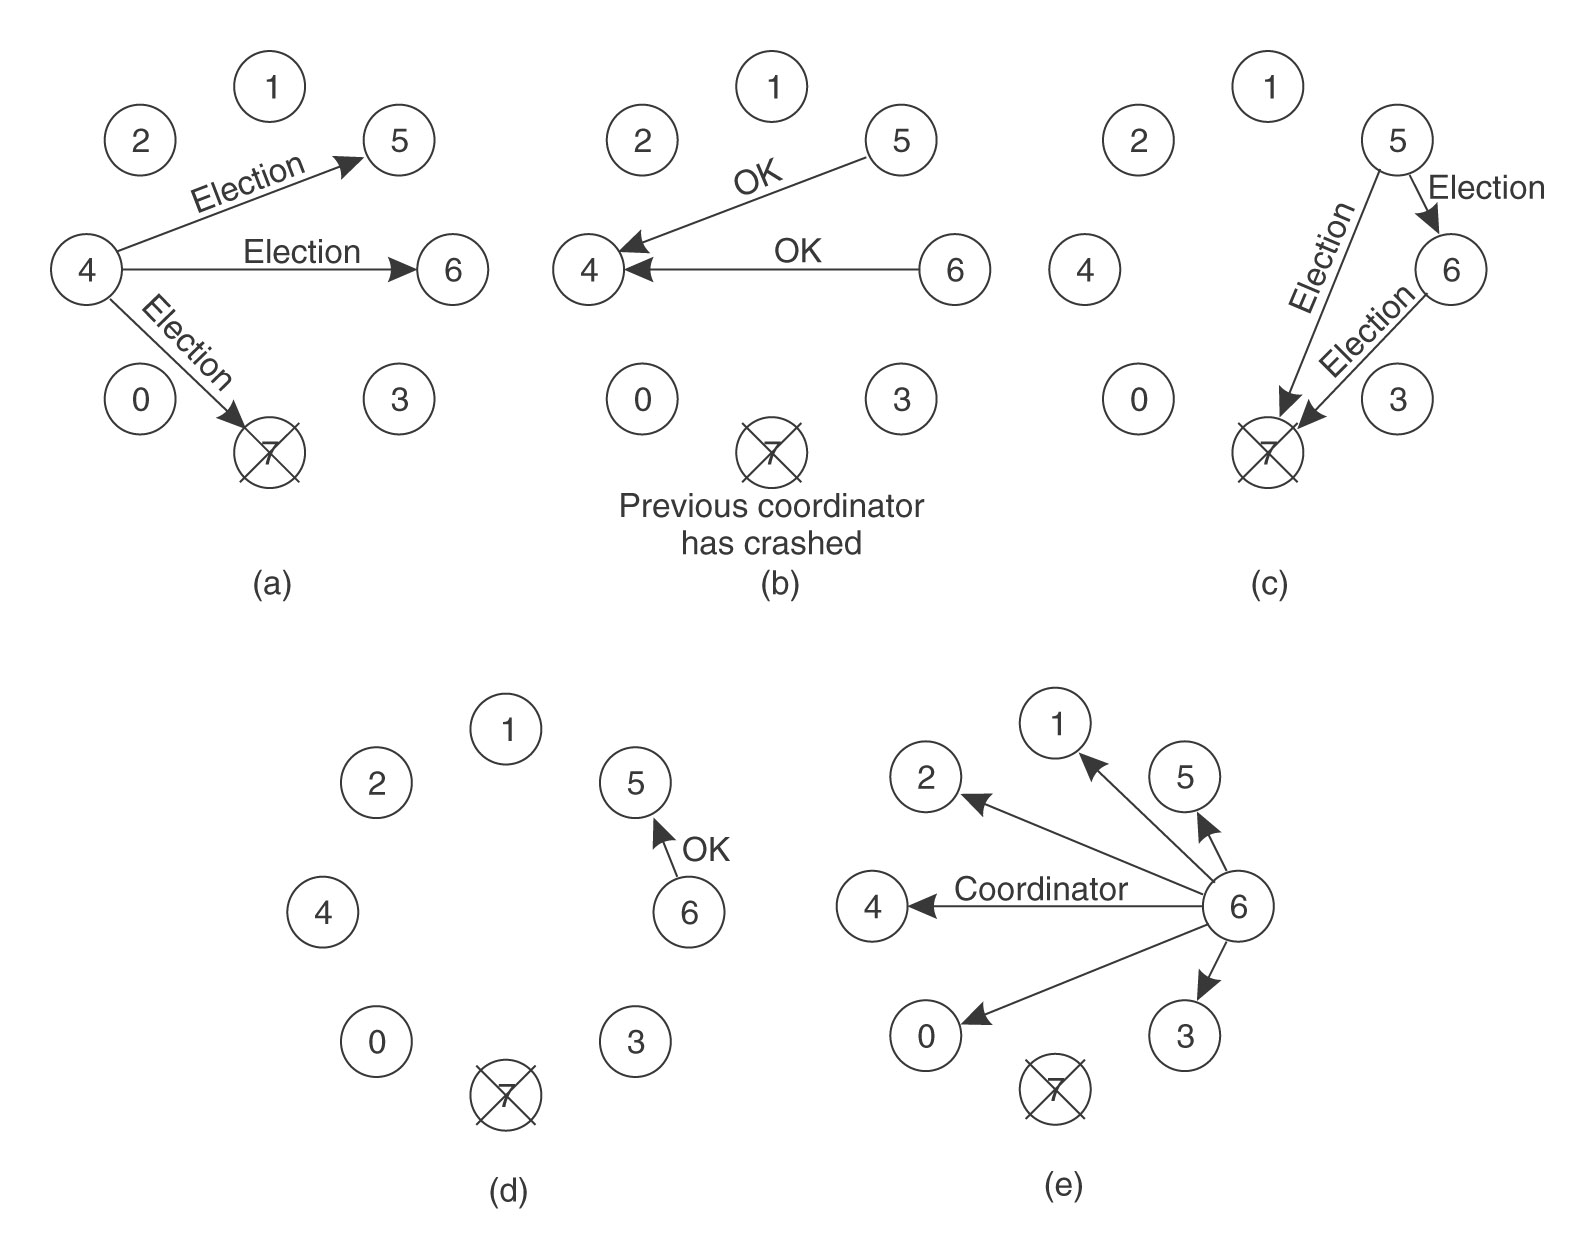
\includegraphics[width=16.5cm]{16/tyran}
\captionof{figure}{Algorytm tyrana}
\end{center}

\item algorytm pierścieniowy (ring algorithm):
    \begin{itemize}
    \item według Tanenbauma
        \begin{center}
        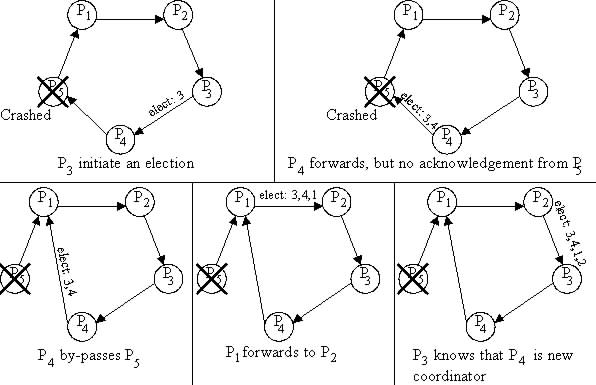
\includegraphics[width=15cm]{16/ring}
        \captionof{figure}{Algorytm pierścieniowy według Tanenbauma}
        \end{center}
            Poniższy rysunek obrazuje działanie algorytmu w~przypadku, gdy~dwa procesy (2~i~5) odkryły, że~koordynator nie~działa i~rozpoczęły dwie równoczesne elekcje.
    
        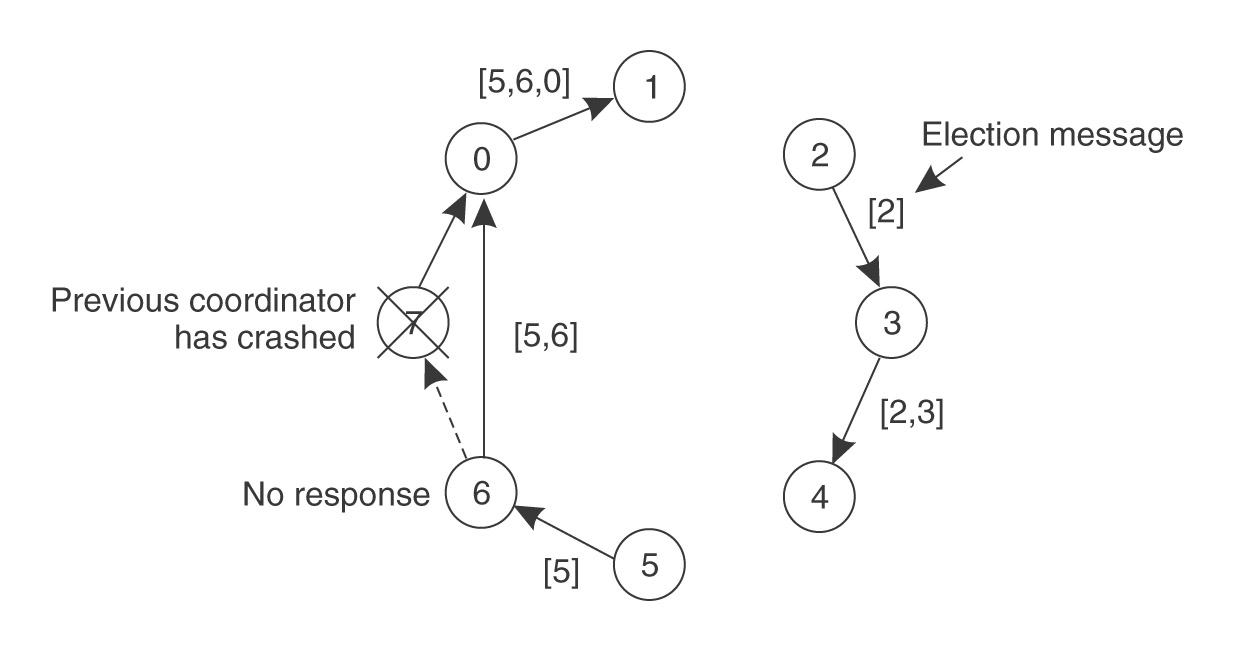
\includegraphics[width=12cm]{16/ring_double_election}
    
    \item według Coulourisa (nie był omawiany przez PTMa)
    
        Aby uniknąć powielania elekcji tak jak w~Tannenbaumie, algorytm Coulourisa wprowadza dodatkową flagę w~każdym z~procesów, która informuje czy~dany proces uczestniczy w~danej chwili w~elekcji.
    
    \end{itemize}
\end{itemize}}

\newpage

\answerC
{Zaznacz prawdziwe zdania}
{Prawo Amdahla pozwala oszacować \underline{teoretyczny} wzrost szybkości systemu przy~zmianie liczby procesorów}
{T}
{\underline{W teorii} prawo Amdahla jest w~stanie oszacować maksymalny wzrost, ale \underline{w~praktyce} wychodzi to~zdecydowanie gorzej.

\noindent
Prawo Amdahla jest używane do~znajdowania maksymalnego spodziewanego zwiększenia wydajności całkowitej systemu jeżeli tylko~część systemu została ulepszona. Jest ono~często używane w~przypadku prowadzenia obliczeń równoległych do~przewidzenia teoretycznego maksymalnego wzrostu szybkości obliczeń przy~użyciu wielu procesorów.

\noindent
Zwiększenie szybkości wykonywania się programu przy~użyciu wielu procesorów w~obliczeniach równoległych jest ograniczane przez~czas potrzebny do~sekwencyjnego dzielenia programu. Na~przykład jeżeli program potrzebuje 20~godzin w~przypadku obliczeń prowadzonych na~procesorze jednordzeniowym i~1~godzina obliczeń nie~może zostać przetworzona poprzez obliczenia równoległe, ale~pozostałe 19 godzin (95\%) obliczeń mogą, wówczas bez~względu na~to~ile~procesorów zostanie użytych do~przeprowadzenia obliczeń równoległych minimalny czas wykonania programu nie~będzie nigdy mniejszy niż~ta~krytyczna 1~godzina. Tak więc zwiększenie szybkości obliczeń jest ograniczone do~20x, jak przedstawiono na~poniższym diagramie:

\begin{center}
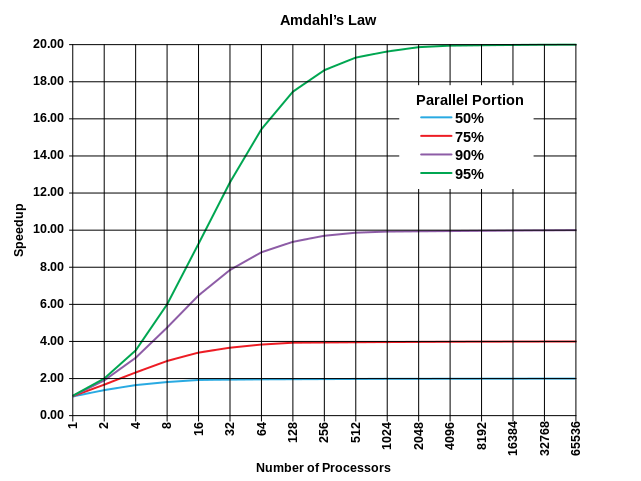
\includegraphics[width=14cm]{16/amdahl}
\captionof{figure}{Prawo Amdahla}
\end{center}}
\chapter{Bazy danych}
\PartialToc % odkomentować przed wysłaniem !!!!!!!!m
\startcontents[chapters]
\printcontents[chapters]{}{1}{\section*{\contentsname}}


%%%%%%%%%%%%%%%%%%%%%%%%%%%%%%%%%%%%%%%%%%%%%%%%%%%%%%%%%%%%%%%%%%%%%%%%%%%%%%%%%%%%
% 279

\answer{Wskaż wszystkie prawdziwe stwierdzenia dotyczące kluczy w~relacyjnym modelu danych.}
{Klucz podstawowy jest zawsze kluczem prostym.}{F}
{Klucz podstawowy może być kluczem prostym albo złożonym}
{\\}

\noindent
Musimy zdefiniować następujące pojęcia:
\begin{description}
   \item[Zbiór identyfikujący] dowolny atrybut lub zbiór atrybutów pozwalający na jednoznaczną identyfikację krotki (rekordu) w relacji (tabeli)
   \item[Klucz] każdy minimalny zbiór identyfikujący, czyli taki że dowolny jego podzbiór właściwy nie jest kluczem (chodzi o to, że nie możemy za pomocą mniejszej ilości atrybutów z tego zbioru uzyskać jednoznaczności przy wyszukiwaniu rekordu)
   \item[Klucz prosty] klucz składający się z tylko jednego atrybutu
   \item[Klucz złożony] klucz składający się z więcej niż jednego atrybutu
   \item[Klucz podstawowy (główny)] wybrany przez użytkownika klucz
   \item[Klucz obcy] atrybut lub ich zestaw występujący w danej relacji, a będący kluczem określonym w innej relacji,
   \item[Atrybut kluczowy] - atrybut wchodzący w skład co najmniej jednego klucza
\end{description}
A więc przykładowa odpowiedź jest błędna, gdyż klucz podstawowy moży być kluczem złożonym. Poprawne stwierdzenia odnośnie kluczy powinny się dać wywnioskować z powyższych definicji. Przykłady:
\begin{enumerate}
\item Jeżeli dla zmiennej relacyjnej istnieje więcej niż jeden klucz, to wszystkie klucze składają się z tej samej liczby atrybutów - Fałsz, ponieważ może instnieć klucz $\{A\}$ i klucz $\{B, C\}$ jednocześnie
\end{enumerate}

% 280

\answer{Dana jest relacja $R$ o schemacie $H = \{A, B, C, D, E, F, G\}$ i zbiorze zależności funkcyjnych $F = \{\{C\}  \rightarrow  \{A\}, \{C\}  \rightarrow  \{B, F\}, \{C\} \rightarrow  \{G\}, \{E\}  \rightarrow  \{C\}, \{G\}  \rightarrow  \{A, B\}\}$. Które z podanych zbiorów są kluczami relacji $R$?}
{$\{A, B, C, D, E, F, G\}$ }{F}
{$\{D, E\}$}
{\\}

\vspace{0.2cm}
\noindent
Aby wyznaczyć wszystkie klucze danej relacji należy policzyć domknięcia tranzytywne wszystkich podzbiorów atrybutów jej schematu $H$. Możemy jednak zauważyć, że atrybuty $D$ i $E$ nie występują po prawej stronie żadnej zależności funkcyjnej. Pozwala to stwierdzić, że muszą się one znajdować w zbiorze będącym kluczem relacji $R$. Liczymy więc domknięcie tranzytywne najmniejszego podzbioru $H$ zawierającego te atrybuty. 

$$
\{D, E\}^+ = \{D, E, C, A, B, F, G\} = H
$$

\noindent
Akurat wyszło nam, że zbiór atrybutów $\{D, E\}$ jest kluczem (bo jego domknięcie tranzytywne jest równe zbiorowi $H$ i żaden z jego podzbiorów właściwych nie jest kluczem). Ponadto możemy stwierdzić, iż nie ma żadnego innego klucza, gdyż każdy pozostały do sprawdzenia zbiór atrybutów zawierałby w sobie atrybuty $D$, $E$ (czyli był nadkluczem).

%%%%%%%%%%%%%%%%%%%%%%%%%%%%%%%%%%%%%%%%%%%%%%%%%%%%%%%%%%%%%%%%%%%%%%%%%%%%%%%%%%%%
% 281
\answer{Dla których z podanych operacji algebry relacji schemat(y) argumentu(ów) i relacji wynikowej $s$, są takie same?}
{rzutowanie}{F}
{selekcja, suma, iloczyn, różnica}
{\\}

\vspace{0.2cm}
\noindent
Algebra relacji pozwala na konstruowanie nowych relacji ze starych. Wyróżniamy następujące operacje algebry: suma, iloczyn (przecięcie), różnica, selekcja, rzutowanie, iloczyn karteziański i złączenia, przemianowanie (zmiana nazwy relacji lub jej atrybutów).

\vspace{0.2cm}
\noindent
Operacje zachowujące schemat(y) relacji: selekcja, suma, iloczyn, różnica \\
Operacje niezachowujące schemat(ów) relacji: rzutowanie, iloczyn karteziański, złączenia, przemianowanie (prośba o weryfikację przemianowania)



\vspace{0.2cm}
\noindent
Uwaga: założono, że w pytaniu chodzi o zachowywanie schematu w każdym przypadku użycia, a nie w szczególnym.

%%%%%%%%%%%%%%%%%%%%%%%%%%%%%%%%%%%%%%%%%%%%%%%%%%%%%%%%%%%%%%%%%%%%%%%%%%%%%%%%%%%%
% 282
\answer{Załóżmy, że w zapytaniu opartym na dwóch relacjach zastępujemy operator złączenia wewnętrznego operatorem złączenia zewnętrznego. Wskaż te operatory, których użycie gwarantuje wynik nie mniejszy (w sensie relacji inkluzji) niż użycie operatora złączenia wewnętrznego.}
{złączenie lewostronne zewnętrzne}{T}
{Patrz poniżej}
{\\}

\vspace{0.2cm}
\noindent
Wyróżniamy 4 rodzaje złączenia zewnętrznego: lewostronne, prawostronne, pełne i typu union. Rozważmy złączenie relacji R i S ($R \Join_{\theta} S$)
\begin{description}
	\item[LEFT OUTER JOIN] wynikiem są wszystkie krotki z R uzupełnione krotkami z S które spełniają warunek $\theta$. Tak jak w złączeniach wewnętrznych dana krotka z R może ulec złączeniu z wieloma krotkami z S. Krotki z R dla których brakuje pasującej krotki z S uzupełniane są nullami
    \item[RIGHT OUTER JOIN] analogicznie do LEFT tylko tutaj relacja S uzupełniana jest krotkami z R
    \item[FULL OUTER JOIN] wynik zawiera wszystkie krotki z R i S. Uzupełniane wartościami null gdy brakuje pasującej krotki w drugiej relacji.
    \item[UNION]  złączenie zawierające wszystkie krotki relacji R nie pasujące do żadnej krotki relacji S uzupełnione tymi krotkami z relacji S które nie pasują do żadnej krotki relacji R.
\end{description}

\vspace{0.2cm}
\noindent
Operatory, których użycie gwarantuje wynik nie mniejszy niż użycie operatora złączenia wewnętrznego: złączenie lewostronne/prawostronne/pełne zewnętrzne

%%%%%%%%%%%%%%%%%%%%%%%%%%%%%%%%%%%%%%%%%%%%%%%%%%%%%%%%%%%%%%%%%%%%%%%%%%%%%%%%%%%%
% 283
\answer{Wskaż, w których przypadkach klauzule instrukcji \textit{select} są ułożone we właściwej kolejności.}
{from, where, group by, having}{T}
{Patrz poniżej}
{\\}

\vspace{0.2cm}
\noindent
Rozszerzona wersja kolejności: 
$$
select ... from ... where ... group~by ... having ... order~by ... limit ... offset  
$$

%%%%%%%%%%%%%%%%%%%%%%%%%%%%%%%%%%%%%%%%%%%%%%%%%%%%%%%%%%%%%%%%%%%%%%%%%%%%%%%%%%%%
% 284

\answer{Wskaż, które elementy dopuszczalne w konceptualnym modelu danych są niekompatybilne z modelem relacyjnym.}
{związki rekurencyjne jeden do jednego}{F}
{Patrz poniżej}{\\}
\noindent
\begin{description}
   \item[Model konceptualny] jest podstawą tworzenia logicznego modelu danych. Składają się na niego: zbiory encji, typy związków, atrybuty i dziedziny atrybutów, klucze i klucze główne, więzy integralnosci.
\end{description}
Elementy niekompatybilne, które należy usunąć przy projektowaniu relacyjnych baz danych to:
\begin{itemize}
  \item związki binarne typu wiele do wielu
  \item związki rekurencyjne typu wiele do wielu
  \item związki złożone
\end{itemize}

% 285

\answer{Dana jest relacja R o schemacie $H = \{A, B, C, D, E, F\}$ i zbiorze zależności funkcyjnych $F = \{\{A\} \rightarrow \{B\}, \{C\} \rightarrow \{D, E\}, \{A, C\} \rightarrow \{F\}\}$. Które z podanych dekompozycji relacji $R$ na relacje o schematach $H_1, H_2 i H_3$ są bezstratne?}
{$H_1 = \{A, B, C\}, H_2 = \{D, E, F\}, H_3 = \{C, D\}$}{F}
{Patrz poniżej}{\\}
\noindent
\begin{description}
   	\item[Dekompozycja] rozbicie relacji na relacje o mniejszej liczbie atrybutów.
	\item[Dekompozycja stratna] gdy ponowne złączenie relacji nie prowadzi do relacji wyjściowej
	\item[Dekompozycja bezstratna] gdy ponowne złączenie relacji prowadzi do relacji wyjściowej
\end{description}
\vspace{0.2cm}
\noindent \textbf{Ogólny algorytm sprawdzania bezstratnosci dekompozycji}
\vspace{0.2cm}

\noindent Niech dany będzie zbiór atrybutów $H = \{A_1,\ldots,A_n\}$ i niech $F$ będzie zbiorem zależności funkcyjnych. Rozważamy dekompozycję relacji $R$ o schemacie $H$ na $k$ relacji $R_i$ o schematach $H_i$.
Konstruujemy macierz S zawierającą k wierszy o etykietach $R_i$ i $n$ kolumn o etykietach $A_j$.
\begin{enumerate}
 	\item Dla kazdego atrybutu $A_j \in H$ i każdej relacji $R_i$, jeżeli $A_j \in H_i$, to umieszczamy znak \Checkmark w komórce $S(i, j)$.
	\item Dla każdej zależności funkcyjnej  $X \rightarrow Y \in F (X, Y \subseteq  H)$, dla kazdych dwóch wierszy macierzy $S$, które mają znaki \Checkmark dla wszystkich kolumn ze zbioru $X$, jezeli którykolwiek z wierszy ma znak \Checkmark w jakiejś kolumnie ze zbioru $Y$, to wstawiamy znak \Checkmark równiez w drugim z rozważanych wierszy dla tej kolumny. 
\end{enumerate}
Jeżeli istnieje wiersz macierzy zawierający znaki \Checkmark we wszystkich swoich komórkach, to dekompozycja jest bezstratna, w przeciwnym przypadku dekompozycja jest stratna.
\vspace{0.2cm}

\noindent\textbf{Dla przykładowej odpowiedzi}
\vspace{0.2cm}

\noindent
\begin{tabular}{|c|c|c|c|c|c|c|} 
\hline
  & $A$ & $B$ & $C$ & $D$ & $E$ & $F$ \\ \hline
$H_1$ & \Checkmark & \Checkmark & \Checkmark & {\color{red} \Checkmark } & & \\ \hline
$H_2$ & & & & \Checkmark & \Checkmark & \Checkmark \\ \hline
$H_3$ & & & \Checkmark & \Checkmark & & \\ \hline
\end{tabular}
\vspace{0.2cm}

\noindent
\Checkmark -- pierwszy krok, {\color{red} \Checkmark} -- drugi krok
\vspace{0.2cm}

\noindent
\textbf{Dekompozycja jest stratna!}
\vspace{0.2cm}

\noindent
\textbf{Przykładowe bezstratne:}
\begin{itemize}
	\item{$H_1 = \{A, B, C, E, F\}, H_2 = \{D, E, F\}, H_3 = \{C, D\}$}
	\item{$H_1 = \{A, B, C\}, H_2 = \{C, D, E, F\}, H_3 = \{A, C, D, F\}$}
\end{itemize}


% 286

\answer{Wskaż wszystkie prawdziwe stwierdzenia dotyczące postaci normalnej Boyce’a–Codda.}
{Dowolna relacja dwuatrybutowa jest w BCNF}{T}
{Patrz poniżej}{\\}
\noindent Niech dana będzie relacja $R$ o schemacie $H = \{A_1,\ldots, A_n\}$ i zbiór zależności funkcyjnych $F$.
Relacja $R$ jest w postaci normalnej Boyce’a–Codda (BCNF) wtw, gdy dla każdej nietrywialnej, prostej zalezności funkcyjnej $X \rightarrow A \in F^+ $, $X$ jest nadkluczem ($X \subseteq H, A \in H$).
\vspace{0.2cm}

\noindent \textbf{Prawidłowe stwierdzenia o BCNF:}
\begin{itemize}
  \item Jeżeli schemat relacji znajduje się w postaci normalnej Boyce’a–Codda, to nie ma w nim redundancji.
  \item BCNF oznacza, ze lewa strona każdej nietrywialnej zależności funkcyjnej zawiera klucz
  \item Dowolna dwuatrybutowa relacja jest w BCNF.
  \item Dowolną relację $R$ o schemacie $H$ można sprowadzić do BCNF stosując dekompozycję bezstratną, ale niekoniecznie zachowującą zalezności funkcyjne.
\end{itemize}

% 287
\answer{Dana jest relacja R o schemacie $H = \left\{A, B, C, D, E\right\}$ oraz zbiór zależnosci funkcyjnych $F = \{\{B, C\} \rightarrow \{D, E\}, \{C, D\} \rightarrow \{B, E\}, \{D\} \rightarrow \{C\}, \{E\} \rightarrow \{B\}\}$. W jakiej maksymalnie postaci normalnej jest relacja $R$? (Zakładamy, ze jest w 1NF.)}
{3NF}{T}
{Patrz poniżej}{\\}
{Aby osądzić, czy dana relacja jest w danej postaci normalnej musimy określić domknięcie zbioru zależności funkcyjnych $F^+$ oraz wyznaczyć wszystkie wystepujące klucze; w tym celu obliczamy domknięcia tranzytywne pozdzbiorów zbioru $F$ oraz zauważamy, że atrybut $A$ nie występuje po prawej stronie żadnej z zależności, więc musi być częścia klucza.} \\ \\
\begin{tabular}{|c|c|c|} 
\hline
	Left & Both & Right \\ \hline
	& $B$ $C$ $D$ $E$ & \\ \hline
\end{tabular} \\ \\
{Ponieważ wszystkie atrybuty (poza atrybutem $A$) występują zarazem po lewej jak i po prawej stronie zależności funkcyjnych, nie pozostaje nam nic innego niż sprawdzić kolejno domknięcia tranzytywne wszystkich podzbiorów owego zbioru atrybutów}
$$ \{B\}^+ = \{B\} $$
$$ \{C\}^+ = \{C\} $$
$$ \{D\}^+ = \{D, C, B, E\}  => \{A, D\}^+ = H $$
$$ \{E\}^+ = \{E, B\} $$
Jedynym odnalezionym dwuelementowym kluczem jest zbiór $\{A, D\}$; mogą jednak istnieć inne klucze, dlatego sprawdzamy domknięcia tranzytywne zbiorów zawierajacyh trzy atrybuty, jednocześnie nie będące nadzbiorem dla $\{A, D\}$
$$ \{B, C\}^+ = \{B, C, D, E\} => \{A, B, C\}^+ = H $$
$$ \{B, E\}^+ = \{B, E\} $$
$$ \{C, E\}^+ = \{C, E, B, D\} => \{A, C, E\}^+ = H $$
{W drugiej turze odnaleźliśmy kolejne dwa klucze: $\{A, B, C\}$ oraz $\{A, C, E\}$; na tym etapie przerywamy juz poszukiwania -- każdy kolejny 4-elementowy zbiór atrubutów byłby nadzbiorem odnalezionych już kluczy.}
{\\}
{Powracając do głównego pytania postawionego w zadaniu należy określić, jakie warunku musi spełniać relacja należąca do danej postaci. Przypomnijmy: \\
Relacja $R$ jest w trzeciej postaci normalnej (3NF) wtw, gdy dla każdej nietrywialnej, prostej zalezności funkcyjnej $X \rightarrow A \in F^+$ $X$ jest nadkluczem lub A nalezy do pewnego klucza relacji $R$ ($X \subseteq H, A \in H$).
\vspace{0.2cm} \\
Jeżeli zatem zauważymy, że wszystkie atrybuty $\{A, B, C, D, E\}$ należą do pewnego klucza, to jesteśmy w stanie od razu stwierdzić, że relacja należy do 3NF (drugi z warunków jest zawsze spełniony)}.
{\\}
{Pozostaje nam jedynie sprawdzić, czy relacja należy również do BCNF. Przypomnijmy: \\
Relacja $R$ jest w postaci normalnej Boyce’a–Codda (BCNF) wtw, gdy dla każdej nietrywialnej, prostej zalezności funkcyjnej $X \rightarrow A \in F^+ $, $X$ jest nadkluczem ($X \subseteq H, A \in H$). \\
Wśród określonych przez nas zależności należących do $F^+$ odnajdujemy jednak zależność $ \{E\} \rightarrow \{B\}$, dla której atrubut $E$ nie jest nadkluczem dla żadnego z istniejących kluczy - zatem relacja nie nalezy do BCNF.}
\noindent

% 288
\answer{Wskaz wszystkie prawdziwe stwierdzenia dotyczące trzeciej postaci normalnej.}
{Dowolną relację mozna sprowadzić do 3NF stosując dekompozycję bezstratną.}{T}
{Patrz poniżej}{\\}
\noindent Relacja $R$ jest w trzeciej postaci normalnej (3NF) wtw, gdy dla każdej nietrywialnej, prostej zalezności funkcyjnej $X \rightarrow A \in F^+$ $X$ jest nadkluczem lub A nalezy do pewnego klucza relacji $R$ ($X \subseteq H, A \in H$).
\vspace{0.2cm}

\noindent \textbf{Prawidłowe stwierdzenia o 3NF:}
\begin{itemize}
  \item 3NF oznacza, że każdy atrybut niekluczowy (informacyjny) zależy wyłącznie od klucza. Innymi słowy, atrybuty informacyjne są wzajemnie niezalezne.
  \item BCNF jest nieco bardziej restrykcyjną wersją 3NF. W BCNF wszystkie atrybuty (równiez kluczowe) muszą spełniać ten warunek. Ten dodatkowy wymóg ma znaczenie, gdy relacja zawiera wiele kluczy.
  \item Jezeli relacja jest w BCNF, to jest również w 3NF.
  \item Jezeli relacja jest w 3NF, to możliwe jest występowanie pewnych redundancji. Postać normalna 3NF jest kompromisem używanym wtedy, gdy nie można uzyskać BCNF.
  \item W praktyce próbujemy uzyskać BCNF, ale ważniejsze jest zachowanie zależności, więc, jesli przejście do BCNF nie zachowuje zależności, wybieramy 3NF.
  \item Dowolną relację $R$ o schemacie $H$ można sprowadzić do 3NF stosując dekompozycję bezstratną i zachowującą zależności funkcyjne. 
  \item Relacja jest w 3NF jeśli jest w 2NF i nie zawiera zależności przechodnich
\end{itemize}

% 289

\answer{Wskaż wszystkie prawdziwe stwierdzenia dotyczące kluczy obcych w relacyjnym modelu danych.}
{Wartosci klucza obcego są unikatowe}{F}
{Patrz poniżej}{\\}
\noindent
\begin{description}
	\item[Klucz obcy] (\textit{foreign key}) w modelu relacyjnym bazy danych to kombinacja jednego lub wielu atrybutów tabeli, które wyrażają się w dwóch lub większej liczbie relacji. Wykorzystuje się go do tworzenia relacji pomiędzy parą tabel, gdzie w jednej tabeli ten zbiór atrybutów jest kluczem obcym, a w drugiej kluczem głównym.
\end{description}
\noindent \textbf{Prawidłowe stwierdzenia o kluczu obcym:}
\begin{itemize}
  \item Klucze obce są sposobem łączenia danych przechowywanych w różnych tabelach
  \item Klucz obcy jest kolumną lub grupą kolumn tabeli, która czerpie swoje wartości z tej samej dziedziny co klucz główny powiązanej z nią tabeli
  \item Klucz obcy musi odnosić się do istniejącej krotki lub przyjmować wartość \textit{null}, aby jawnie stwierdzić, że nie ma związku z reprezentowanymi obiektami w bazie danych albo że ten związek jest nieznany
  \item Klucz obcy \textbf{nie musi} być unikatowy w obrębie tabeli
  \item Klucz obcy może pochodzić z tej samej tabeli, gdy chcemy utworzyć związek rekurencyjny 
  \item Odwołania klucz obcy – klucz mozna definiować na poziomie \textbf{kolumny} tylko wtedy, gdy powiązane klucze są kluczami prostymi (zawierają jeden atrybut). W PSQL Używamy do tego słowa kluczowego \textbf{\textit{references}}, np.\\
\lstinline[columns=fixed]{idksiazki char(4) not null references ksiazki,} 
\item Odwołania klucz obcy – klucz definiowane na poziomie \textbf{tabeli} pozwalają łączyc ze sobą klucze złożone, np.\\
\lstinline[columns=fixed]{foreign key (numer, idkategorii) references elementy} 
\item Zarówno klucz główny, jak i obcy mogą miec nazwy nadane przez programistę (w miejsce nazw generowanych przez system zarządzania bazą danych), np.\\
\lstinline[columns=fixed]{constraint klucz_obcy}\\ 
\hspace*{1.2cm}\lstinline[columns=fixed]{foreign key (numer, idkategorii) references elementy} 

	\item W przypadku zdefiniowania zalezności między dwoma kluczami, usunięcie lub modyfikacja wartosci (klucza) w tabeli nadrzędnej ma wpływ na tabelę podrzędnę.
Definiując powiązanie mozna określić, jak system zarządzania bazą danych ma się w takiej sytuacji zachować. Odpowiednie reguły ograniczeń dla kluczy obcych dodaje się
na końcu definicji ograniczenia\\
\lstinline[columns=fixed]{references tabela [(kolumna)] [on delete akcja] [on update akcja]}\\ 

Akcje:
\begin{itemize}
	\item restrict -– zapobiega usunięciu/modyfikacji rekordu z tabeli nadrzędnej, jezeli istnieje odwołanie do tego rekordu;
	\item no action -– (akcja domyslna) zgłoszenie błędu, przy próbie usunięcia/modyfikacji rekordu z tabeli nadrzędnej, jezeli istnieje odwołanie do tego rekordu; w przeciwienstwie do poprzedniej akcji sprawdzanie może być odroczone do końca transakcji;
	\item cascade -– kaskadowe usuwanie/modyfikacja rekordów w tabeli podrzędnej;
	\item set null -– ustawia wartość klucza obcego na null;
	\item set default -– ustawia wartosć klucza obcego na wartość domyślną.
\end{itemize}
\end{itemize}

% 290

\answer{Wskaż wszystkie prawdziwe stwierdzenia dotyczące użycia funkcji agregujących w systemie PostgreSQL.}
{Klauzula \textit{group by} słuzy do podziału na rozłączne podzbiory krotek będących wynikiem selekcji.}{T}
{Patrz poniżej}{\\}
\noindent
\textbf{Podstawowe funkcje agregujące:}
\begin{description}
   \item[count(*)] liczba wierszy spełniających określone (w klauzuli where) warunki 
   \item[count(x)] liczba wierszy, w których wartość w kolumnie x jest różna od null
   \item[avg(x)] średnia arytmetyczna wartości w kolumnie x
   \item[max(x)] maksymalna wartość w kolumnie x
   \item[min(x)] minimalna wartość w kolumnie x
   \item[stddev(x)] odchylenie standardowe wartości w kolumnie x
   \item[sum(x)] suma wartości w kolumnie x
   \item[variance(x)] wariancja wartości w kolumnie x
\end{description}

\noindent \textbf {Zdania prawdziwe na temat funkcji agregujących:} 
\begin{itemize}
	\item Dostają na wejściu zbiór wartości, a zwracają tylko jedną wartość.
	\item Są obliczane po uprzednim obliczeniu klauzuli where, dlatego nie mogę one w niej wystapić; jedyną możlwiością pośredniego użycia wyniku funkcji agregującej w klazuli where jest stworzenie podzapytania:
niepoprawnie: [...] WHERE punkty > avg(punkty) 
poprawnie: [...] WHERE punkty > (SELECT avg(punkty) FROM wyniki))
	\item mogą występować w liście SELECT dla kolumn nie wsytępujących w klauzuli GROUP BY
	\item wówczas wynikiem będzie jedna wartość dla każdej grupy utworzonej przez klauzulę GROUP BY
	\item mogą byc użyte w klauzuli HAVING
	\item ignorują wartość null.
	\item Poza funkcją count, dla zerowej liczby wierszy wszystkie funkcje agregujące zwrócą null (np. sum() nie zwróci 0).
	\item W przypadku stosowania funkcji min i max do kolumn typu varchar ciągi porównywane są po uprzednim uzupełnieniu ich z prawej strony spacjami.
	\item Funkcje sum i avg przyjmują jako argument kolumnę o typie numerycznym.
\end{itemize}


% 291
\answer{Wskaż wszystkie prawdziwe stwierdzenia dotyczące transakcji.}
{Transakcja jest ciągiem operacji w bazie danych, które nalezy wykonać wszystkie lub nie wykonywać żadnej z nich.}{T}
{Patrz poniżej}{\\}
\noindent \textbf {Zdania prawdziwe na temat transakcji:} 
\begin{itemize}
	\item Transakcja rozpoczyna sie słowem kluczowym BEGIN, a kończy słowem kluczowym END
	\item{
    	Transakcja może zakończyć swoje działanie na cztery sposoby:
    	\begin{itemize}
    		\item COMMIT - pomyslne zakończenie transakcji i zatwierdzenie wszystkich zmian
        	\item ROLLBACK - wycofanie wszystkich zmian przeprowadzonych w ramach transakcji
        	\item może zostać abortowana przez SZBD z powodu zakleszczenia
    		\item może zostać przerwana z powodu awarii serwera lub dysku
    	\end{itemize}
    } 
	\item PostgreSQL nie zezwala na zagnieżdżanie transakcji (próba wpisania BEGIN podczas trwania transakcji poskutkuje komunikatem "transakcja jest w toku")
    \item{
    	Transakcje obowiązują własności ACID, czyli transakcja jest:
    	\begin{itemize}
    		\item Niepodzielna (Atomic) – mimo że jest zbiorem działan, musi być wykonywana jako pojedyncza, odbywająca sie w jednym momencie i nie dzieląca na pozdbiory jednostka. 
        	\item Spójna (Consistent) – po zakonczeniu jej wykonywania system musi być spójny.
        	\item Odizolowana (Isolated) – jest niezależna od innych wykonujących się w danym momencie transakcji
    		\item Trwała (Durable) – po wykonaniu musi zostać utrwalona (w PostgreSQL wykonuje się to za pomocą pliku dziennika transakcji)
    	\end{itemize}
    }
    \item Podczas wykonywania transakcji może wystąpic problem brudnych danych i brudnego odczytu; Brudne dane to dane zapisane w transakcji, ale jeszcze nie zatwierdzone. Brudny odczyt to odczyt brudnych danych zapisanych przez inną transakcje; zazwyczaj użytkownik ma możliość zablokowania/odblokowania odczytu brudnych danych, jednak w W PostgreSQL odczyt brudnych danych nie jest możliwy
    \item Stopień wzajemnej separacji transakcji jest określony za pomocą "poziomu izolacji"; 
    \item Transakcje powinny być niewielkie
    \item W przypadku konieczności otrzymania danych od uzytkownika, dobrą szkołą jest uprzednie zebranie wszystkich wartości a następnie zapisanie ich wszystkich razem za pomoca transakcji
\end{itemize}
    
\textbf {Istniejące poziomy izolacji transakcji:}
\begin{description}
\item[read committed (odczyt zatwierdzony)] nie można odczytać brudnych danych, ale można zobaczyć zmiany zatwierdzone w między czasie przez inne transakcje, tj. w ramach transakcji wykonanie tego samego zapytania wielokrotnie może dawać inne wyniki
\item[repeatable read (odczyt powtarzalny)] gwarancja, że po pobraniu krotki
po raz pierwszy, w przypadku ponowienia zapytania otrzymamy identyczną krotkę
\item[serializable (odczyt uszeregowany)] Poziom ten wyklucza możliwość wystąpienia wszystkich omawianych zjawisk niepożądanych
\end{description}
 

% 292
\answer{Wskaż, które ograniczenia można definiować na poziomie kolumny (w instrukcji \textit{create table}).}
{wartość domyślną atrybutu}{T}
{Patrz poniżej}{\\}
\noindent
(Opcjonalne) ograniczenia dla kolumny pozwalają określić dla niej dodatkowe (poza obligatoryjnem typem - typ nie jest ograniczeniem) reguły.
\textbf {Możliwe do określenia ograniczenia dla kolumn:}
\begin{itemize}
	\item not null – w kolumnie nie mogą byc zapisywane wartosci null;
	\item unique – wartosci zapisywane w kolumnie muszą być różne dla każdego wiersza w
tabeli;
	\item primary key – połaczenie ograniczeń null oraz unique (Uwaga: tworzenie złożonego klucza podstawowego jest możliwe tylko przy użyciu ograniczeń na poziomie tabeli)a poziomie tabeli;
	\item default wartość - zdefiniowanie wartości domyślnej;
	\item check (warunek) – warunek sprawdzany w czasie wprowadzania lub aktualizacji
danych;
	\item references – ograniczenia kluczy obcych.
\end{itemize}



% 293
\answer{Wskaż wszystkie prawdziwe stwierdzenia dotyczące wartości \textit{null}}
{Wartosci \textit{null} są różne od spacji, zera czy też pustego łańcucha znaków.}{T}
{Patrz poniżej}{\\}
\noindent\textbf{Stwierdzenia prawdziwe dla wartości null:}
\begin{itemize}
	\item Wartosci null to tzw. wartości puste, reprezentują one brak wartości danego atrybutu
(chwilowy lub permanentny)
	\item W pewnych okolicznosciach (np. wyświetlanie, porządkowanie), wartości null są traktowane jak każde inne
	\item W pewnych okolicznościach nie podlegają przetwarzaniu i dają nieokreślone wartości funkcji
    \item Dwie wartości null nie są traktowane jako równe. Porównanie wartosci null z dowolną wartością daje wartoć logiczną unknown lub null (różną od true i false).
	\item W związku z powyższym, porównanie z wartością null realizujemy za pomocą konstrukcji:
wyrażenie is null/ wyrażenie is not null
	\item Null może zastapić dowolną wartość, nie należy bowiem do żadnego typu
	\item Podstawowa regułą matematyczna jest ich propagacja - działanie arytmetyczne zawierające null da w wyniku null
	\item Chociaż nie można porównywac ze sobą dwóch wartości null, to w kontekście klauzul group by, order by i distinct wartość null jest traktowana jako identyczna z inną wartością null lub jako jej duplikat.
	\item Jeżeli podzapytanie skalarne nie zwraca ąadnej krotki, to jako jego wynik
przyjmowana jest wartość null.
	\item null może wystąpic jako wartość wstawiana
	\item W PostgreSQL element tablicy nie może być null (tablica tak).
\end{itemize}



\chapter{Lingwistyka formalna i~automaty}
\PartialToc
%\startcontents[chapters]
%\printcontents[chapters]{}{1}{\section*{\contentsname}}

%294
\answer
{Gramatyka jest wieloznaczna, jeżeli:}
{Jest to gramatyka kontekstowa lub bezkontekstowa}
{F}
{Gramatyka wieloznaczna to gramatyka, której język zawiera przynajmniej jedno zdanie wieloznaczne.}
{Gramatyka wieloznaczna to gramatyka, której język zawiera przynajmniej jedno zdanie wieloznaczne. Gramatyka nie zawierająca  zdania wieloznacznego to gramatyka jednoznaczna. \\
Zdanie wieloznaczne to zdanie, dla którego  istnieje więcej niż jedno drzewo syntaktyczne wyprowadzania takiego zdania. Cechę jednoznaczności lub wieloznaczności przypisujemy gramatyce,a nie językowi przez nią generowanemu. Często dla danego języka możemy wyprowadzić zarówno gramatykę wieloznaczną,jak i jednoznaczną. Istnieją jednak także języki,dla których zdefiniowanie gramatyki jednoznacznej nie jest możliwe. Nazywamy je językami istotnie wieloznacznymi.
}

%295
\answer
{(K\_W15, K\_W03, K\_W04, K\_W07, K\_U15, K\_U21, K\_U22, K\_U03, K\_U04) Które z poniższych napisów są prawdziwe dla języka generowanego przez następującą gramatykę $G = \langle\{Q, P, X\}, \{\bigtriangledown, \bigtriangleup\}, \{X \to \bigtriangledown \bigtriangleup R, X \to \bigtriangleup \bigtriangledown Q, R \to \bigtriangleup \bigtriangledown X, R \to \bigtriangleup \bigtriangledown, Q \to \bigtriangledown \bigtriangleup X, Q \to \bigtriangledown \bigtriangleup\}, X \rangle$: (zakładam, że $P$ i $R$ to to samo... po prostu pomyłka, w innym przypadku zadanie trochę bez sensu)}
{$\bigtriangledown \bigtriangleup \bigtriangleup \bigtriangleup \bigtriangleup \bigtriangledown \bigtriangledown \bigtriangledown \bigtriangledown \bigtriangleup \bigtriangleup \bigtriangleup$}
{F}
{$\bigtriangledown \bigtriangleup \bigtriangleup \bigtriangledown$ lub $\bigtriangleup \bigtriangledown \bigtriangledown \bigtriangleup$ lub napisy który mają na początku: $\bigtriangledown \bigtriangleup \bigtriangleup \bigtriangledown$ $\vee$ $\bigtriangleup \bigtriangledown \bigtriangledown \bigtriangleup$, a kolejne symbole są parami różne albo co najwyżej dwa obok siebie sa takie same (najlepiej sprawdzać jak w wyjaśnieniu)}
{\\$\{Q, P, X\} \in N$ - symbole nieterminalne\\
	$\{\bigtriangledown, \bigtriangleup\} \in T$ - symbole terminalne\\
	produkcje: $\{X \to \bigtriangledown \bigtriangleup R,\\ 
	X \to \bigtriangleup \bigtriangledown Q,\\
	R \to \bigtriangleup \bigtriangledown X,\\
	R \to \bigtriangleup \bigtriangledown,\\
	Q \to \bigtriangledown \bigtriangleup X,\\
	Q \to \bigtriangledown \bigtriangleup\}$\\
	$X \in N$ -symbol startowy

	\begin{description}
		\item $X \to$ \textbf{(a)} $\bigtriangledown \bigtriangleup R$ $\vee$ \textbf{(b)} $\bigtriangleup \bigtriangledown Q$ - symbol startowy $X$ może przejść w dwa stany: \textbf{(a)} lub \textbf{(b)}:
		\item[ad. (a)] $\bigtriangledown \bigtriangleup (R) \to$ \textbf{(aa)} $\bigtriangleup \bigtriangledown X$ $\vee$ \textbf{(ab)} $\bigtriangleup \bigtriangledown$ - w \textbf{(a)} na końcu jest symbol $R$, który również może przejść w dwa stany: \textbf{(aa)} lub \textbf{(ab)}:
		\begin{description}
			\item[ad. \textbf{(aa)}] ma na końcu $X$, więc przechodzimy znowu do stanu \textbf{(a)} lub \textbf{(b)}, a początek napisu wygląda następująco: $\bigtriangledown \bigtriangleup \bigtriangleup \bigtriangledown$, po czym następuje \textbf{(a)} $\bigtriangledown \bigtriangleup (R)$ lub \textbf{(b)} $\bigtriangleup \bigtriangledown (Q)$ itp.,
			\item[ad. (ab)] daje napis $\bigtriangledown \bigtriangleup \bigtriangleup \bigtriangledown$.
		\end{description}
		\item[ad. (b)] $\bigtriangleup \bigtriangledown (Q) \to$ \textbf{(ba)} $\bigtriangledown \bigtriangleup X$ $\vee$ \textbf{(bb)} $\bigtriangledown \bigtriangleup$ - w \textbf{(b)} na końcu jest symbol $Q$, który przechodzi w jeden z dwóch stanów: \textbf{(ba)} lub \textbf{(bb)}:
		\begin{description}
			\item[ad. (ba)] ma na końcu $X$, więc znowu przechodzimy do stanu \textbf{(a)} lub \textbf{(b)}, a początek napisu wygląda następująco: $\bigtriangleup \bigtriangledown \bigtriangledown \bigtriangleup$, po czym następuje \textbf{(a)} $\bigtriangledown \bigtriangleup (R)$ lub \textbf{(b)} $\bigtriangleup \bigtriangledown (Q)$ itp.,
			\item[ad. (bb)] powstaje napis $\bigtriangleup \bigtriangledown \bigtriangledown \bigtriangleup$.
		\end{description}
	\end{description}
	}
	
%296
\section{K\_W15}\label{296}
\textbf{296. Dla domkniecia Kleene’ego prawdziwe sa nastepujace stwierdzenia:}\\
przykładowa odp.) jest to zbiór słów powstały przez konkatencje dwóch domknietych dodatnio jezyków\\
\textbf{FAŁSZ}

Domknięcie Kleene'ego L* języka L jest najmniejszym spośród zbiorów X spełniających\\
\begin{enumerate}
	\item $\varepsilon \in X$
	\item $L \subseteq X$
	\item jeżeli $s \in X$ oraz $x \in L$, to $sx \in X $
\end{enumerate}

\textbf{Dodatnie} domknięcie Kleene'ego $L^+$ definiujemy jako najmnieszy spośród zbiorów X spełniających\\
\begin{enumerate}
	\item $L \subseteq X$
	\item jeżeli $s \in X$ oraz $x \in L$, to $sx \in X $
\end{enumerate}

Przykładowo:\\\\
$V = \{ba, ca\}$\\
$V* = \{\varepsilon, ba, ca, baba, baca, caca, caba, babaca, ...\}$\\
$V^+ = \{ba, ca, baba, baca, caca, caba, babaca, ...\}$

%297
\answer{(K\_W15) Zapis $L^* = \bigcup_{i=0}^{\infty} L^i$ oznacza dla języków:}
{operację skończonego sumowania języków}
{F}
{domknięcie Kleene'ego}
{patrz zad. \ref{296}}

%298
\answer
{Dla klasyfikacji gramatyk Chomsky'ego prawdziwe są następujące stwierdzenie}
{Praktyczne znaczenie dla możliwości konstruowania kompilatorów języków programowania mają gramatyki klasy 2 i 3}
{T}
{}
{\\jeżeli gramatyka jest typu $i$, to jest również typu $j$, dla $j \leq i$\\
	\begin{tabular}{|c|c|c|c|}
		\hline
		JĘZYK & GRAMATYKA & HIERARCHIA CHOMSKY'EGO & AUTOMAT\\
		\hline
		\multirow{2}{*}{regularny} & regularna  & \multirow{2}{*}{3} & skończony \\
			& liniowa & & Rabina-Scotta \\
		\hline
		bezkontekstowy & bezkontekstowa & 2 & ze stosem\\
		\hline
		\multirow{2}{*}{kontekstowy} & kontekstowa  & \multirow{2}{*}{1} & \multirow{2}{*}{liniowo-ograniczony} \\
		& monotoniczna & & \\
		\hline
		rekurencyjnie przeliczalny & kombinatoryczna & 0 & maszyna Turinga\\
		\hline
	\end{tabular}
	\begin{itemize}
		\item typ $0$ - rekurencyjnie przeliczalny podzbiór zbioru wszystkich słów nad danym alfabetem,
		\item typ $2$ - języki bezkontekstowe mają ważne znaczenie w informatyce, m.in. w budowie kompilatorów,
		\item typ $3$ - lewostronnie regularne lub prawostronnie, za pomocą tych gramatyk opisuje się składnię większości podstawowych elementów leksykalnych języków programowania (identyfikatory, stałe numeryczne, stałe tekstowe itp.)
		
	\begin{tabular}{|c|c|c|c|c|}
		\hline
		\multirow{2}{*}{JĘZYK} & \multirow{2}{*}{CZY $x \in L$?} & \multirow{2}{*}{CZY $L(G) = \emptyset$?}  & CZY $G$ JEST & CZY\\
		& & & JEDNOZNACZNA? & $L(G_1) = L(G_2)$?\\
		\hline
		regularny & tak  & tak  & tak & tak \\
		\hline
		bezkontekstowy & tak & tak & nie & nie\\
		\hline
		kontekstowy & tak & nie & nie & nie\\
		\hline
		rekurencyjnie & \multirow{2}{*}{nie} & \multirow{2}{*}{nie} & \multirow{2}{*}{nie} & \multirow{2}{*}{nie}\\
		przeliczalny & & & &\\
		\hline
	\end{tabular}		
	\end{itemize}
	
}

%299
\answer
{(K\_W15, K\_W03, K\_W04, K\_W07, K\_K01, K\_K06) Dla języków i gramatyk formalnych, odnośnie postaci normalnej Chomsky’ego oraz postaci normalnej Greibach można sformułować następujące stwierdzenia (duże litery alfabetu łacińskiego to symbole nieterminalne, a litery małe to symbole nieterminalne)  (małe litery to raczej symbole terminalne...)}
{dla każdego języka bezkontekstowego istnieje gramatyka w postaci normalnej Chomsky’ego}
{F}
{\textit{Chomsky:} $A \to a$, $A \to BC$, \textit{Greibach:} $A \to aX$, języki generowane przez gramatyki w obu postaciach nie zawierają słowa pustego, każdą gramatykę bezkontekstową (bez słowa pustego) można przedstawić w obu postaciach, każdą gramatykę bezkontekstową w postaci \textit{Chomsky'ego} można przekształcić do postaci \textit{Greibach}}
{\\ Postać normalna \textit{Chomsky'ego} - produkcje wyglądają następująco:\\
	$A \to a$, $A \to BC$, gdzie duże litery to symbole nieterminalne, a małe terminalne\\
	\newline
	Każdą gramatykę bezkontekstową (gramatyki generują języki) niegenerującą symbolu pustego można przekształcić do postaci normalnej \textit{Chomsky’ego}. Żeby rozszerzyć ten zbiór do wszystkich gramatyk bezkontekstowych, rozszerza się czasem postać normalną \textit{Chomsky’ego} o reguły: $S \in \epsilon$ ($S$ – symbol startowy, $\epsilon$ – słowo puste), ale gramatyka zawierająca taką regułkę nie może zawierać $S$ po prawej stronie żadnej reguły.\\
	\newline
	Postać normalna \textit{Greibach}:\\
	$A \to aX$ ($a$ - dowolny symbol terminalny, $X$ - ciąg symboli nieterminalnych (może być pusty))\\
	\newline
	- języki generowane przez gramatyki w obu postaciach nie zawierają słowa pustego,\\
	- każdą gramatykę bezkontekstową (bez słowa pustego) można przedstawić w obu postaciach,\\ 
	- każdą gramatykę bezkontekstową w postaci \textit{Chomsky'ego} można przekształcić do postaci \textit{Greibach}.}

%300
\section{K\_W15, K\_U15, K\_U21, K\_U22}
\textbf{300. Odnośnie lematu o pompowaniu dla języków regularnych prawdziwe są:}\\
przykładowa odp.) lemat słuzy pokazaniu, że określone języki są regularne\\
\textbf{FAŁSZ}\\

Twierdzenie służy do dowodzenia, że dany język \textbf{nie} jest językiem regularnym\\\\
Twierdzenie brzmi:\\
Jeżeli dany język $L$ jest regularny, to istnieje takie $n \geq 1$, że każde słowo w należące do $L$ długości co najmniej $n$ można podzielić na trzy części $xyv$, gdzie $y$ jest niepuste i $|xy| < n$, w taki sposób, że dla każdego $k \geq 0$ słowo postaci $xy^kv$ należy do danego języka.

%301
\answer{(K\_W15, K\_K01, K\_K06) Jeżeli $Lin$ oznacza gramatyki liniowe, $BK$ gramatyki bezkontekstowe, $Reg$ gramatyki regularne, $PL$ gramatyki prawostronnie liniowe, a $LL$ gramatyki lewostronnie liniowe, to które z następujących relacji są prawdziwe:}
{$Lin \subseteq BK$}
{T}
{}
{\\$BK(LL) \subseteq Reg \subseteq Lin \subseteq BK$\\
	$BK \cap LL = Reg$\\
	\newline
	$Lin$ (gramatyki liniowe) - takie, które po lewej stronie reguł mają pojedyncze nieterminale, po prawej zaś słowa zawierające co najwyżej jeden nieterminal (jeśli znajduje się on na początku lub na końcu każdego słowa – jest to odpowiednio gramatyka lewostronnie lub prawostronnie liniowa).\\
	\newline
	$Reg$ (gramatyki regularne) - to gramatyka formalna, za pomocą której można opisać język regularny. Istnieją dwa rodzaje gramatyk regularnych: gramatyka lewostronna, gramatyka prawostronna. Istnieje ścisły związek gramatyki lewostronnej oraz deterministycznego automatu skończonego, taki że gramatyka generuje dokładnie taki język jaki akceptuje automat. Stąd gramatyki lewostronne generują dokładnie wszystkie języki regularne. Gramatyka regularna to albo prawo albo lewostronna.}

%302
\answer
{Które ogólne stwierdzenia odnośnie języków, gramatyk i automatów są prawdziw}
{Jeżeli $L$ jest językiem regularnym, to istnieje automat deterministyczny ze stosem akceptujący ten język }
{F}
{Jeżeli $L$ jest językiem regularnym, to istnieje automat skończony akceptujący ten język}
{
	\begin{itemize}
		\item Jeżeli $L$ jest językiem rekurencyjnie przeliczalnym - to istnieje maszyna Turinga akceptująca ten język
		\item Jeżeli $L$ jest językiem kontekstowym, to istnieje automat liniowo ograniczony akceptujacy ten język
		\item Jeżeli $L$ jest językiem bezkontekstowym, to istnieje automat niedeterministyczny ze stosem akceptujący ten język
		\item Jeżeli $L$ jest językiem regularnym, to istnieje automat skończony akceptujący ten język
	\end{itemize}
}

%303
\answer{(K\_W15, K\_W03, K\_W04, K\_W07, K\_U15, K\_U21, K\_U22) Dla danego ustalonego języka $L$ i alfabetu $V$, językiem ilorazowym $L/x$ nazywamy język postaci:
	$$L/x = \{y \in V^*: xy \in L\}$$
	dla $x \in V^{*}$. Które stwierdzenia są prawdziwe:}
{jezeli język $L$ jest regularny, to istnieje nieskończenie wiele języków ilorazowych}
{F}
{jezeli język $L$ jest regularny, to istnieje skończenie wiele języków ilorazowych}
{\\Jeżeli $A$ będzie ustalonym językiem:\\
	 język $A$ jest regularny $\Leftrightarrow$ istnieje skończenie wiele języków ilorazowych języka $A$\\
	 jest ich co najwyżej tyle, co stanów osiągalnych w deterministycznym automacie skończonym akceptującym $A$}

%304
\section{K\_W15, K\_W03, K\_W04, K\_W07, K\_U15, K\_U21, K\_U22, K\_U03, K\_U04}
\textbf{304. $\varepsilon$-domknięciem E dla stanu początkowego $q_1$ dla przedstawionego ponizej automatu są zbiory}

\begin{figure}[h!]
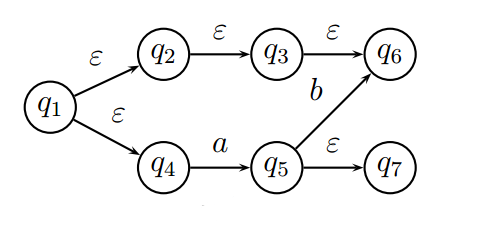
\includegraphics[scale=0.5]{18/automata.png}
\end{figure}

przykładowa odp.) $E(q_1) = \emptyset$; – tj. nie da się wyznaczyc ze względu na puste przejścia\\
\textbf{FAŁSZ}\\\\

$\varepsilon$-domknięcie stanu $q E(q)$ definiuje się:
\begin{enumerate}
\item Podstawa: Stan $q$ należy do $E(q)$
\item Krok indukcyjny: Jeżeli stan $p$ należy do $E(q)$ oraz istnieje przejście ze stanu $p$ do stanu $r$ o etykiecie $\varepsilon$, to $r$ należy do $E(q)$ - jeżeli funkcją przejścia opisywanego NAS jest $\delta$ i $p$ należy do $E(q)$, to $E(q)$ zawiera także stany z $\delta(p, \varepsilon)$.
\end{enumerate}

Dla zadanego automatu $E(q) = \{q_1, q_2, q_3, q_4, q_6\}$


%305
\answer{(K\_W15, K\_W03, K\_W04, K\_W07, K\_U15, K\_U21, K\_U22) Dany jest automat niedeterministyczny $A = \{S = \{A,B,C\}, V = \{0,1\}, \{\delta(A,1) = B, \delta(A,1) = C, \delta(B,0), \delta(C,0) = B\}, s_0 = A, Z = \{C\}\}$. Automat po determinizacji (w znaczeniu algorytmu Rabina-Scotta) będzie miał:}
{osiem stanów}
{F}
{cztery stany}
{\\
	Stworzenie deterministycznego automatu skończonego z niedeterministycznego automatu skończonego jest zawsze możliwe i otrzymany w tym procesie automat akceptuje dokładnie ten sam język, co automat wejściowy. Jeżeli niedeterministyczny automat ma $n$ stanów, wynikowy deterministyczny może mieć do $2^n$ stanów.\\
	\newline
	$S = \{A,B,C\}$ - zbiór stanów\\
	$V = \{0,1\}$ - alfabet\\
	$\delta(A,1) = B, \delta(A,1) = C, \delta(B,0), \delta(C,0) = B$ - funkcje przejścia\\
	$s_0 = A$ - stan początkowy\\
	$Z = \{C\}$ - stany końcowe (akceptujące)\\
	Powyższy automat wygląda jak na rysunku \ref{a}.\\
	\newline
	Automat skończony, deterministyczny i zupełny nazywamy deterministycznym automatem Rabina-Scotta.\\
	Automat skończony $A$ jest deterministyczny i zupełny $\Leftrightarrow$\\($\forall s\in S: \#\delta(s,\epsilon) = 0$) $\wedge$ ($\forall a \in V: \forall s \in S: \#\delta(s,a) = 1$)\\
	\newline
	Maksymalna liczba stanów w deterministycznym automacie wynosi $2^3 = 8$.\\
	Tworzymy automat z $8$ stanami, tak żeby z każdego stanu wychodziła jedna strzałka z $1$ oraz jedna z $0$ (rys. \ref{b}):\\
	$S' = \{\alpha, \beta, \gamma, \alpha\beta, \alpha\gamma, \beta\gamma, \alpha\beta\gamma, \omega\}$:\\
	$\alpha$ odpowiada stanowi $A$, $\beta$ - $B$, $\gamma$ - $C$,\\ 
	$\omega$ - jeżeli z któregoś stanu nie istnieje przejście dla $1$ lub $0$ do innego stanu, wtedy przejście jest do $\omega$,\\ 
	każdy ze stanów $\alpha\beta, \alpha\gamma, \beta\gamma, \alpha\beta\gamma$ odpowiada za wszystkie stany, które zawiera, tzn. np. dla stanu $\beta\gamma$ z $A$($\alpha$) można przejść($1$) zarówno do $B$($\beta$) jak i do $C$($\gamma$), to znaczy, że istnieje połączenie($1$) z $\alpha$ do $\beta\gamma$; ani z $B$ ani z $C$ nie ma przjeścia dla $1$, więc z $\beta\gamma$ dla $1$ jest przejście do $\omega$, natomiast $0$ jest osiągalne z $B$ do $A$ oraz z $C$ do $B$, więc z $\beta\gamma$ jest strzałka($0$) do $\alpha\beta$. I tak postepujemy dla wszystkich nowych stanów tworząc połączenia.\\
	$V' = \{0,1\}$ - nic się nie zmienia\\
	funkcje przejścia widać na rysunku \ref{b}\\
	$s_0' = \alpha$ - nowy stan początkowy\\
	$Z' = \{\gamma, \alpha\gamma, \beta\gamma, \alpha\beta\gamma\}$ - wszystkie stany, które zawierają $\gamma$($C$)\\
	\newline
	Ostatnią rzeczą jest usunięcie stanów, do których nie da się przejść ze stanu początkowego(są one bezużyteczne), czyli zaczynając od stanu $\alpha$ sprawdzamy do których stanów istnieje ścieżka. Gotowy graf przedstawia rysunek \ref{c} - $4$ stany.
	
	
	\begin{figure}[h]
%		\includegraphics[width=0.3\textwidth]{naut}
%		\includegraphics[width=0.3\textwidth]{daut1}
%		\includegraphics[width=0.3\textwidth]{daut2}
		\centering
		\begin{subfigure}[b]{0.3\textwidth}
			\includegraphics[width=\textwidth]{18/naut}
			\caption{automat niedeterministyczny}
			\label{a}
		\end{subfigure}
		\begin{subfigure}[b]{0.3\textwidth}
			\includegraphics[width=\textwidth]{18/daut1}
			\caption{automat po determinizacji z nieosiągalnymi stanami}
			\label{b}
		\end{subfigure}
		\begin{subfigure}[b]{0.3\textwidth}
			\includegraphics[width=\textwidth]{18/daut2}
			\caption{automat po determinizacji bez nieosiągalnych stanów}
			\label{c}
		\end{subfigure}
	\end{figure}
}

%306
\answer
{Jeżli $r$ oraz $s$ są wyrażeniami regularnymi dla języków odpowiednio $R$ oraz $S$, to $(r+s)$, $rs$ i $r^*$ są wyrażeniami regularnym reprezentującymi odpowiednio}
{ $R \cup S$, $R \times S$ i $R^+$}
{F}
{$R \cup S$, $R \times S$ i $R^*$}
{
	$(r+s) \rightarrow r | q$, oznacza sumę teoriomnogościową języków $R$ i $S$. $R \cup S = \{x | x \in R \lor x \in S\}$ \\
	$rs$, oznacza złożenie (konkatenację) języków $R$ i $S$. $R \times S = \{rs | r \in R, s \in S\}$ \\
	$r^*$, oznacza domknięcie Kleene'go języka $R$. $R^* = R^0 \cup R^1 \cup R^2 \cup ...$  
}

%307
\answer{(K\_W15, K\_W03, K\_W04, K\_W07, K\_U15, K\_U21, K\_U22) Wyrażenie regularne $(0 + 1)^*00(0 + 1)^*$ opisuje:}
{łańcuchy rozpoczynające się zerem a kończące jedynką}
{F}
{wszystkie łańcuchy skłądające się z zer i jedynek, zawierające podciąg $00$}
{\\$a + b$ - alternatywa a i b (a lub b)\\
	$^*$ - domknięcie Kleene'ego\\ 
	$ab$ - złożenie a i b (litery występują razem w tej kolejności)\\
	$a^* = \{\epsilon, a, aa, aaa, ...\}$\\
	$(a + b)^* = \{\epsilon, a, aa, b, bb, ab, ba, abb, ...\}$ - każde możliwe słowo składające się z liter a i b}

%308
\section{K\_W15, K\_W03, K\_W04, K\_W07, K\_U15, K\_U21, K\_U22}
\textbf{308. Mamy języki $L_1 = \{ a^{2^n} : n > 0\}$ oraz $L_2 = \{ a^{2n} : n > 0\}$. Które z tych języków są regularne? }\\
przykładowa odp.) $L_1$ -- tak, $L_2$ -- tak\\
\textbf{FAŁSZ}\\\\

\textbf{Język regularny} -- język formalny taki, że istnieje automat o skończonej liczbie stanów potrafiący zdecydować, czy dane słowo należy do języka.\\\\

Wykorzystując lemat o pompowaniu należy pokażać, że język jest nieregularny. Dla $L_1$:\\
\begin{enumerate}
	\item Wybieramy x,y,z takie, że : $x=\varepsilon, y=a^{2^{k}-1}, z=a$
	\item Słowo składa się wyłącznie z liter $a$ oraz $0<|v|<2^k$
	\item Dla $i=2$ słowo $xuv^2wz \notin L_1 $, bo $2^k < |xuv^2wz| < 2^{k+1}$
\end{enumerate}
Zatem $L_1$ jest językiem nieregularnym

\chapter{Teoria kompilacji i kompilatory}
\PartialToc
%\startcontents[chapters]
%\printcontents[chapters]{}{1}{\section*{\contentsname}}

\answer
{Typowy skaner języka formalnego ma za zadanie}
{Zliczyć lewe i prawe nawiasy sprawdzając wstępnie ich sparowanie}
{F}
{Wczytać kod źródłowy programu do postaci tokenów, innymi słowy - wykonuje analizę leksykalną.}
{\textbf{Według wykładu Klimka, skaner:}

\begin{itemize}
\item wyodrębnia podstawowe symbole języka zwane \textit{atomami} lub \textit{tokenami}
\item usuwa znaki nie mające wpływu na sam program, np. odstępy, tabulacje,
\item usuwa komentarze umieszczone w programie,
\item dane wejściowe to postać pośrednia programu źródłowego zawierająca atomy wraz z krótkim opisem
\end{itemize}}

\answer
{Typowy parser języka formalnego ma za zadanie}
{Wstępnie przydzielić adresy zmiennym kontrolnym pętli programu źródłowego}
{}
{Parser, nazywany też analizatorem syntaktycznym, dokonuje rozbioru syntaktycznego. Powinien odtworzyć wywód oraz go zapamiętać (np. przez kolejne numery produkcji). Parser korzysta z wcześniej zdefiniowanej gramatyki.}
{\textbf{Według wykładu Klimka}, parser ma na celu sprawdzenie poprawności syntaktycznej przez:

\begin{itemize}
\item dokonanie rozbioru programu na części składowe,
\item zbudowanie odpowiedniego drzewa składniowego
\end{itemize}
\textbf{Dodatkowo:}
Parser można podzielić na:
\begin{itemize}
\item \textit{analizator syntaktyczny} - dokonuje ścisłej analizy składniowej,
\item \textit{analizator semantyczny} - sprawdza pewne aspekty poprawności semantycznej(np. wielokrotna deklaracja tej samej zmiennej, a także inne).
\end{itemize}
}

\answer
{Przez rozbiór kanoniczny rozumiemy rozbiór, który:}
{W pierwszej kolejności redukuje prawostronne symbole formy zdaniowej}
{F}
{Jest to rozbiór, który zawsze rozpoczyna redukcję formy zdaniowej od lewej strony}
{}
%\section{K\_W15, K\_W03, K\_W04, K\_W07, K\_W20, K\_K01, K\_K06}

\answer
{Metoda generacyjna rozbioru gramatycznego polega na tym, że:}
{Rozpoczynając od symbolu początkowego gramatyki usiłuje się przejść do napisu wejściowego}
{T}
{Polega na tym, że rozpoczynamy analizę od ``najbardziej ogólnego'' elementu gramatyki (symbolu startowego) i dążymy do otrzymania terminali pasujących do analizowanej formy gramatycznej}
{\textbf{Według wykładu Klimka:}

Metoda \textit{generacyjna} polega na tym, iż rozpoczynając od symbolu startowego gramatyki, korzystając ze wszystkich jej produkcji, próbuje się utworzyć końcowy cel analizy, tzn. wygenerować analizowany ciąg symboli. Analiza ta zwana jest także \textit{zstępującą}, ze względu na fakt rozpoczęcia analizy od symbolu początkowego i posuwania się w analizie w dół, tj. budowania drzewa syntaktycznego od jego korzenia do liści.}
%\section{K\_W15, K\_W03, K\_W04, K\_W07, K\_W20, K\_U24}

\answer
{Metoda redukcyjna rozbioru gramatycznego polega na tym, że:}
{Rozpoczynając od symbolu początkowego gramatyki usiłuje się przejść do napisu wejściowego}
{F}
{Polega na próbie otrzymania symbolu początkowego gramatyki wychodząc od napisu wejściowego.}
{\textbf{Według wykładu Klimka:}

Metoda \textit{redukcyjna} polega na tym, iż rozpoczynając od analizowanego ciągu symboli sprawdza się możliwości zredukowania go do symbolu początkowego gramatyki korzystając z jej produkcji. Analiza ta zwana jest także \textit{wstępującą}, ze względu na fakt prowadzenia analizy od liści drzewa syntaktycznego i posuwania się do góry w stronę jego korzenia.

\textbf{Dodatkowo}: Do analizy generacyjnej można stosować algorytmy zarówno z \textit{wolymi} jak i z \textit{szybkimi powrotami}. Ograniczeniem analizatorów generacyjnych jest to, iż zasadniczo nie pozwalają na lewostronną rekursję języków. Wymaga to albo przekształcenia produkcji, albo modyfikacji analizatora. W analizie generacyjnej warto zwrócić uwagę na kolejność, a także postać samych produkcji. Jeśli chodzi o kolejność -- wskazane jest by produkcje opisujące ten sam symbol, a którycj prawe strony są przedrostkami innych produkcji, następowały po tych innych produkcjach. Jeśli chodzi o postać produkcji -- to należy unikać produkcji o tych samych przedrostkach, np.
$$ E \rightarrow Ba $$
$$ E \rightarrow Bb $$
}
%\section{K\_W15, K\_W03, K\_W04, K\_W07, K\_W20, K\_U24}

\answer
{Dla analizatorów klasy $LL(k)$ prawdziwe są następujące stwierdzenia}
{Parametr k oznacza liczbę symboli wejsciowych używanych do podejmowania decyzji w każdym kroku pracy}
{T}
{(314==315)\\
\begin{itemize}
\item Odtwarzamy wywód lewostronny
\item k - ilość tokenów używanych do określenia dalszej ścieżki
\item nie wykonują nawrotów (no tak mi się przynajmniej wydaje, bo niby w którym etapie analizy są wykonywane nawroty)
\end{itemize}

\textbf{Dane o analizatorze $LL(k)$}
\begin{itemize}
\item Analizator generacyjny ze stosem,
\item pierwsza liera $L$ odnosi się do kierunku analizowania wejścia (od lewej do prawej),
druga litera $L$ do wywodu(wywód lewostronny),
\item $k$ wskazuje ile symboli wprzód musi być podglądanych aby jednoznacznie określić produkcję niezbędną do poprowadzenia wywodu,
\item analizatory pracują w sposób deterministyczny,
\item Gramatyki $LL(k)$ są jednoznaczne,
\item Przed budowaniem parsera $LL(k)$ należy z gramatyki usunąć lewostronną rekursję,
\item Rekursją prawostronna jest dopuszczalna dla analizatrów typu $LL(k)$,
\item bład składniowy rozpoznawany jest bezpośrednio po natrafieniu na symbol, który nie należy do programu poprawnego,
\item ceną takiego analizatora jest gramatyka o odpowiednich własnościach pozwalająca zrealizować determizm (Sprawdzenie gramatyki pod tym kątem jest stosunkowo łatwe i może odbywać się recznie),
\item O analizatorach $LL(k)$ mówimy, że nie znają historii (może być to uznawane za słabość w porównaniu z np. analizatorami klasy $LR(k)$),
\item związane z analizatorem $LL(k)$ : $PRFX_{k}$ i $FOLLOW_{k}$ (Pozwalają na wyznaczenie odpowiednio prefiksów i następników łańcuchów symboli).
\end{itemize}
}
{}

\answer
{Usunięcie $\epsilon$-produkcji z gramatyki klasy $G_{LL(k)}$ powoduje}
{Zwiększenie wartości parametru $k$ w tej gramatyce/parserze}
{T}
{W analizatorach typu $LL(k)$ $\epsilon$-produkcje gramatyki są dopuszczalne, jednak warto produkcje takie zastąpić produkcją pojedyńczą. Można również w ogóle usunąć $\epsilon$-produkcje.

}
{\textbf{Twierdzenie}

Dla każdej gramatyki $G$ można skonstruować gramatykę $G'$ bez $\epsilon$-produkcji taką, że $L(G') = L(G)\setminus \{ \epsilon \}$
Jeżeli gramatyka $G$ jest $LL(k)$, to $G'$ jest $LL(k+1)$. }
%\section{K\_W15, K\_W03, K\_W04, K\_W07, K\_W20, K\_U24}

\answer
{W odniesieniu do parserów klasy $LR(k)$ prawdziwe są następujące ogólne stwierdzenia:}
{Na stosie trzymane są prefiksy i sufiksy form zdaniowych, co do których jest nadzieja na ich wykorzystanie}
{F}
{Na stosie trzymane są odwiedzone stany automatu parsującego

\textbf{Troszke o $LR(k)$}:
\begin{itemize}
\item Gramatyka bezkontekstowa nazywana jest gramatyką $LR(k)$, jeżeli istneje dla niej parser $LR(k)$,
\item Parser $LR$ wykonuje analizę metodą wstępującą (\textit{bottom-up}), ponieważ próbuje wyprowadzić produkcję najwyższego poziomu poprzez analizowanie liści.
\item paresery $LR$ są trudne do ręcznego zaprogramowania, dlatego są one zwykle konstruowane przez generator parserów,
\item budowa parsera:
    \begin{itemize}
    \item bufor \textit{wejścia},
    \item stos na którym przechowywana jest lista stanów, w których był automat,
    \item \textit{tabela goto} w której opisane jest, do którego nowego stanu powinniśmy przejść,
    \item \textit{tabela action} daje regułę gramatyki do zastosowania w bieżącym stanie i dla aktualnego symbolu terminalnego w strumieniu wejściowym,
    \item parser $LR$ czyta strumień wejściowy od lewej do prawj, ale potrzebuje wyprowadzić prawostronne wyprowadzenie, używa \textbf{redukcji} zamiast wyprowadzeń do przetwarzania strumienia wejściowego (Oznacza to, że algorytm działa tworząc "lewostronną redukcję" wejścia). Końcowym rezultatem po odwróceniu będzie prawostronne wyprowadzenie,
    \item ważne pojęcie w parserach $LR$ - sytuacja (\textit{en.item}) (symbol kropki dodawanej na którymś miejscu po prawiej stronie w produkcji np. $E \rightarrow E\bullet + B$). używane w celu określenia stanu parsera.(Zazwyczaj nie można opisać stanu parsera pojedyńczą sytuacją, ponieważ może on nie wiedizeć z wyprzedzeniem, którą regułę będzie używał do redukcji.
    \end{itemize}
\end{itemize}

Algorytm działania:

\begin{enumerate}
\item Stos jest inicjowany przez [0]. Bieżącym stanem będzie zawsze ten stan, który jest na szczycie stosu
\item Biorąc bieżący stan i bieżący symbol terminalny w strumieniu wejściowym, akcja jest brana z tabeli action (tabela action opisana w pytaniu niżej)
\item Krok 2 jest powtarzany dotąd aż strumień zostanie zaakceptowany lub zostanie zgłoszony błąd składni
\end{enumerate}
}
{}

\answer
{W odniesieniu do pracy parserów klasy $LR(k)$ i funkcji action prawdziwe są stwierdzenia:}
{funkcja $action$ przyjmuje wartości ze zbioru $\{shift, reduce, accept, error\}$}
{T}
{
% o LR można przenieść do pytania wyżej
% i, o szumiący borze, ale żeś się upisała! :D
% teraz mi strasznie wstyd, że tak mało zrobiłem :(
% hahaha, panie ja nie czytam komentarzy :)
% spoko loko, akurat to miałam pod ręką, jak człowiek chodzi na drugie terminy, to cos mu tam po nich zostaje.
Tabela action -- daje regułę gramatyki do zastosowania w bieżącym stanie i dla aktualnego symbolu terminalnego w strumieniu wejściowym.
\\
\textbf{Tabela \textit{action}}. Mamy 4 przypadki:
\begin{itemize}
\item{przesunięcie(\textit{shift}) $s_{n}$:}
    %tak nie lepiej?
    \begin{itemize}
    \item bieżący symbol terminalny jest usuwany ze strumienia wejściowego,
    \item stan \textit{n} jest wkładany na stos i staje się bieżącym stanem.
    \end{itemize}
    %\subitem *bieżący symbol terminalny jest usuwany ze strumienia wejściowego,
    %\subitem *stan \textit{n} jest wkładany na stos i staje się bieżącym stanem.
\item{redukcja(\textit{en.reduce}) \textit{rm}:}
    \begin{itemize}
    \item liczba \textit{m} oznaczająca numer reguły wyprowadzenia jest wpisywana do strumienia wyjściowego,
    \item dla każdego symbolu(terminalnego lub nieterminalnego) z prawej strony reguły \textit{m} stan jest usuwany ze stosu,
    \item biorąc stan który jest następnie na szczycie stosu i symbol nieterminaly, któy jest po lewej stronie \textit{m}, nowy stan jest brany z tabeli \textit{goto} i staje się nowym bieżącym stanem przez włożenie go na stos.
    \end{itemize}
    %\subitem *liczba \textit{m} oznaczająca numer reguły wyprowadzenia jest wpisywana do strumienia wyjściowego,
    %\subitem *dla każdego symbolu(terminalnego lub nieterminalnego) z prawej strony reguły \textit{m} stan jest usuwany ze stosu,
    %\subitem *biorąc stan który jest następnie na szczycie stosu i symbol nieterminaly, któy jest po lewej stronie \textit{m}, nowy stan jest brany z tabeli \textit{goto} i staje się nowym bieżącym stanem przez włożenie go na stos. 
\item{akceptacja(\textit{en.accept}) \textit{acc} -- strumień symboli terminalnych jest zaakceptowany,}
\item{brak akcji(\textit{en. error}) \textit{err} -- zgłaszany jest błąd syntaktyczny.}
\end{itemize}
}
{}

\answer
{Dla tablic sterujących parserów klasy $LR(0)$ i przykładowej produkcji $A \rightarrow XYZ$ mamy:}
{Cztery możliwe sytuacje minus przypadki gdy z danego symbolu po prawej stronie wyprowadzamy tylko symbol pusty}
{T}
{W przypadku tego pytania, sytuacje będą takie:
\begin{enumerate}
\item $A \rightarrow \bullet XYZ$
\item $A \rightarrow X\bullet YZ$
\item $A \rightarrow XY\bullet Z$
\item $A \rightarrow XYZ\bullet$
\end{enumerate}
Jeżeli któryś z symboli będzie dawał tylko symbol pusty, wtedy sytuacji będzie mniej, np. przy założeniu, że $X \rightarrow \epsilon$, sytuacje będą takie:
\begin{enumerate}
\item $A \rightarrow \bullet YZ$
\item $A \rightarrow Y\bullet Z$
\item $A \rightarrow YZ\bullet$
\end{enumerate}
}
{}

\answer
{Budowa tablic sterujących dla analizatorów klasy $LR$ może stwarzać pewne trudności, szczególnie w zakresie automatyzacji, co ma pośredni wpływ na istnienie
wielu odmian tych parserów. Które z poniższych prostych stwierdzeń są poprawne:}
{pierwsze litery w nazwie $LALR$ oznaczają $Look Ahead$}
{T}
{\begin{itemize}
\item wspomniane odmiany to:
    \begin{enumerate}
    \item $SLR$ - Simple $LR$ (jeżeli nie pojawia się k, to jest to $SLR(1)$)
    \item $LALR$ - Look Ahead $LR$ - potrafi przetwarzać gramatyki niebędące $LR(0)$ wymagając takiej ilości stanów co $LR(0)$
    \item $GLR$ - General $LR$ - umożliwia obsługę niedeterministycznych i niejednoznacznych gramatyk
    \end{enumerate}
\end{itemize}

Normalnie w parserach $LR(0)$ w tablicy parsingu akcje redukcji muszą zajmować cały wiersz tabeli powodując to, ze redukcja wykonana jest niezależnie od następnego symbolu w strumieniu wejściowym. Z tego powodu tabele $LR(0)$ nie zaglądają w przód przed decyzją, której redukcji użyć. 
\\~\\
Gramatyka, która potrzebuje spojrzeć w przód aby wybrać redukcję będzie potrzebowała tabeli parsingu, której wiersz będzie zawierał różne akcje redukcji w różnych kolumnach. 
\\~\\
Prcedury konstruujące $SLR$ lub $LALR$ mają możliwość tworzenia wierszy tabeli dla których akcja redukcji nie zajmuje całych wierszy. Dlatego parsery te mają możliwość analizy większej ilości gramatyk niż $LR(0)$.
\\~\\
Automat($LR(0)$) konstruowany jest w sposób, który gwarantuje determinizm. Jednak kiedy akcje redukcji są dodawane do tabeli \textit{action}, może się zdarzyć, że ta sama komórka jest wypełniona przez akcję redukcji i akcję przesunięcia (\textit{konfilkt przesunięcie-redukcja}) lub przez dwie różne akcje redukcji(\textit{konflikt redukcja-redukcja}. Kiedy to się zdarza, to znaczy, że gramatyka nie jest $LR(0)$.

\begin{itemize}
\item $E \leftarrow 1 E $ (akcja przesunięcia)
\item $ E \leftarrow 1 $ (akcja redukcji)
\end{itemize}
konflikt przesunięcie redukcja, ponieważ w komórce tabeli action dla stanu i symbolu '1' jest jednocześnie możliwe przesunięcie stanu i redukcja regułą 2. Rozwiązaniem dla tego problemu może być zastosowanie zboiru \textit{FOLLOW} takie rozwiązanie jest charakterystyczne dla parsera $SLR$.
\\~\\
Parser $SLR$ to parser typu $LR$, jego tabela parsingu kostruowana jest na podstawie kanonicznej rodziny zbiorów sytuacji $LR(0)$ oraz zbiorów $FOLLOW$ dla gramatyki \textit{G}. Sam parser różni się od innych parseró typu $LR$ sposobem konstrukcji(i zazwyczaj zawartością) tej tablicy, natomiast sam algorytm analizy jest identyczny. Jeśli w tabeli parsingu istnieje konfilkt to znaczy, że powstąły parser nie jest deterministyczny i w zasadzie do celów praktycznych sie nie nadaje i trzeba albo zmodyfikować gramatyke albo zastosować lepszy generator (np. $LALR$).  Problemem parserów $SLR$ jest to, że wyznaczenie zbioru \textit{look-ahead} jest zbyt uproszczone, ponieważ używa jedynie reguł gramatyki. Dokladniejsze zbiory \textit{look-ahead} są nazywane zbiorami parsingu $LALR$.
\\~\\
Zaletą $SLR$ w porównaniu z $LALR$ jest łatwość konstrukcji, płaci się za to zmniejszeniem ilości rozpoznawanych gramatyk, gdyż dosyć często interesujące gramatyki nie są $SLR$, natomiast są już $LALR$.
}
{}

\answer
{Dla pewnej gramatyki mówimy, że sytuacja $LR(0)$ oznaczona $[N \rightarrow \beta_1\bullet\beta_2]$ dla $\gamma \in V^*$ jest poprawna, gdy przy założeniu $\alpha\beta_1 = \gamma$ prawdziwe jest:}
{$S \xRightarrow{rm*} \alpha N \omega \Rightarrow \alpha \beta_1 \beta_2 \omega$}
{}
{Według moich notatek z wykładu Klimka poprawne jest coś takiego:
$S \xRightarrow{rm*} \alpha N \omega \Rightarrow \alpha \overset{*}{\beta_1} \beta_2 \omega$
%Tylko czy ta gwiazdka ma znaczenie? Pamiętam, że wykład prowadził Piwowarczyk i on nie miał pojęcia co ta gwiazdka tak właściwie oznacza...
%brzmi jak Klimek, nie? ;)
%stawiam ze ta gwiazdka odnosi sie do sytuacji, albo...do aktualnie analizowanego symbolu, nie iwem...
\\
(Pytanie dziwne...) Wyjaśnijmy użyte symbole:
\\
$S$ -- zwyczajowo zawsze bedzie oznaczać symbol startowy Gramatyki,
\\
$rm*$ -- oznacza ciąg redukcji (0 lub więcej), które do tej pory zastosowaliśmy,
\\
$\omega$ -- słowo, string, zawiera 1 lub więcej symboli terminalnych,
\\
$\alpha, \beta$ -- podciągi słowa może zawierać terminale i nieterminale.
\\
$\gamma$ -- aktywny prefiks gramatyki $G$, $\gamma$ prefiks łańcucha $\alpha\beta_{1}$
\\
$v$ -- symbol terminalny lub koniec strumienia(dolar), nazywany symbolem podglądanym(lookahead).
\\
Aktywny prefiks - łańcuch będący prefiksem pewnej prawostronnie wyprowadzalnej formy zdaniowej, nie wychodzący poza prawy koniec jej osnowy(Każdy wiersz tablicy parsingu $LR(1)$(czyli stan) odpowiada pewnemu aktywnemu prefiksowi).
\\
Sytuacja: $[N \rightarrow \beta_{1}\bullet\beta_{2}, v]$ jest dopuszczalna dla aktywnego prefiksu $\alpha\beta_{1}$ wtedy i tylko wtedy gdy:
\\
$S \xRightarrow{rm*} \alpha N \omega \Rightarrow \alpha\beta_{1} \beta_2 \omega$ oraz $v \in FIRST_{k}(\omega)$
\\
w związku że dla $LR(0)$ nie trzeba podglądać kolejnych symboli można uprościc do:
$N \rightarrow \beta_{1}\bullet\beta_{2}$ jest dopuszczalna dla aktywnego prefiksu $\alpha\beta_{1}$ wtedy i tylko wtedy gdy:
\\
$S \xRightarrow{rm*} \alpha N \omega \Rightarrow \alpha\beta_{1} \beta_2 \omega$
\\
UWAGI:
\begin{enumerate}
\item ponieważ $\beta_1$ może być $\epsilon$, więc dla każdego prefiksu aktywnego istnieje co najmniej jedna $LR(k)$ - sytuacja dopuszczalna,
\item $LR(k)$ - sytuacje postaci $[A \rightarrow \beta\bullet, v]$ są szczególnie ważne gdyż pokazują możliwe redukcje (analiza dobiegła do prawego końca osnowy).
\end{enumerate}
}
{}
%http://kompilatory.agh.edu.pl/pages/tk-wyklady/2-3-Parser-LR(1)-czesc-1.htm

\answer
{Pomiędzy parserami $LR$ zachodzą następujące relacje w odniesieniu do zbiorów gramatyk:}
{$LR(0) \subset SLR(1) \subset LALR(1) \subset LR(1)$}
{T}
{$SLR(1)$ tworzy tablicę stanów jak $LR(0)$ oraz zbiory First oraz Follow bazując na gramatyce. Jest to uproszczone podejście przez co istnieje możliwośc wygenerowania konfiktów, które nie istnieją w tablicy stanów $LR(0)$

$LALR(1)$ również tworzy tablicę stanów jak $LR(0)$ oraz wylicza ``look-ahead'' (właściwie nazwę można zapisać jako $LA(1)LR(0)$ czyli - do look-ahead używa jednego tokenu oraz wykorzystuje tablicę $LR(0)$) bazując na tablicy stanów $LR(0)$}
{}

%https://stackoverflow.com/questions/2676144/what-is-the-difference-between-lr-slr-and-lalr-parsers

\answer
%{K\_W15, K\_W03, K\_W04, K\_W07, K\_W20, K\_U24}
{Porównując gramatyki $LL$ oraz $LR$ można powiedzieć, że:}
{Gramatyki $LR$ opisują szerszą klasę niż $LL$}
{T}
{Każdy gramatyka $LL(k)$ jest również gramatyką $LR(k)$, która z kolei jest zawsze gramatyką bezkontekstową.
Gramatyka $LL(1)$ bez $\epsilon$ jest również gramatyką $SLR(1)$.}
{(z angielskiej wikipedii):
The $LL(1)$ languages are a proper subset of the $LR(1)$ languages which in turn are a proper subset of all context-free languages.

Every $LL(k)$ grammar is also a $LR(k)$ grammar. It is also decidable if a given $LR(k)$ grammar is also a $LL(m)$ grammar for some $m$. A $\epsilon$-free $LL(1)$ grammar is also a $SLR(1)$ grammar. A $LL(1)$ grammar with symbols that have both empty and non-empty derivations is also a $LALR(1)$ grammar. A $LL(1)$ grammar with symbols that have only the empty derivation may or may not be $LALR(1)$.

$LR$ parsers can handle a larger range of languages and grammars than precedence parsers or top-down $LL$ parsing}


%The LL(1) languages are a proper subset of the LR(1) languages which in turn are a proper subset of all context-free languages.

%Every LL(k) grammar is also a LR(k) grammar. It is also decidable if a given LR(k) grammar is also a LL(m) grammar for some m.[4] A ε-free LL(1) grammar is also a SLR(1) grammar. A LL(1) grammar with symbols that have both empty and non-empty derivations is also a LALR(1) grammar. A LL(1) grammar with symbols that have only the empty derivation may or may not be LALR(1).

%LR parsers can handle a larger range of languages and grammars than precedence parsers or top-down LL parsing

\chapter{Podstawy sztucznej inteligencji}
\PartialToc
%\startcontents[chapters]
%\printcontents[chapters]{}{20}{\section*{\contentsname}}
\section{EKK\_1, EKK\_3}
\textbf{Który (które) z poniższych algorytmów zapewniają znalezienie najkrótszej ścieżki w grafie (koszt każdego łuku równy 1):}
\vspace{0.4cm}

\noindent Według ang. wik najczęsciej używane toi:

\begin{itemize}
\item Dijkstra
\item Bellmann-Ford
\item A*
\item Floyd-Warshall
\item Johnson
\item Viterbi
\end{itemize}

Dodatkowo prawdopodobnie:
\begin{itemize}
\item Przeszukiwanie wszerz (ang. breadth-first search, BFS)
\item Przeszukiwanie w głąb (ang. Depth-first search, w skrócie DFS)
\end{itemize}

\section{EKK\_1,EKK\_2}
\textbf{Algorytm Tree-Search Breadth-First F wygenerował 400 węzłów do głębokosci 3.  Szacunkowy (zastępczy) branching factor b wynosi:}
\vspace{0.4cm}

\noindent Effective branching factor - srednia ilosć dzieci wygenerowanych przez "przeciętny" węzeł dla danego przeszukiwania.\\
Definicja:\\
N: całkowita ilosć węzłów\\
d: głębokosć drzewa\\
b: Effective branching factor\\
$N = b* + (b*)^2 + \ldots + (b*)^d$\\
Do przybliżonych obliczeń effective branching factor można przyjąć następujący wzór:\\
$b* = \sqrt[d]{N}$\\
Dla naszego zadania:\\
N = 400\\
d = 3\\
$b* = \sqrt[3]{400} = 7,37$

\section{EKK\_1,EKK\_2}
\textbf{Aby algorytm A* znajdował rozwiązanie optymalne w literaturze przytaczane są następujące wymagania co do funkcji heurystycznej h(n):}
\vspace{0.4cm}

\begin{itemize}
\item the branching factor is finite (each node has only a finite number of neighbors)
\item arc costs are greater than some $\epsilon > 0$
\item h(n) is a lower bound on the actual minimum cost of the lowest-cost path from n to a goal node
\end{itemize}

\noindent Heurystyka h(n) musi być dopuszczalna (ang. admissible), tzn. jej wartosć zawsze jest mniejsza od lub równa najkrótszej rzeczywistej długosci scieżki.

\section{EKK\_1,EKK\_2}
\textbf{Algorytmy  Genetyczne  (AG)  stosowane  są  do  optymalizacji  złożonych  funkcjonałów,  w  tym  problemów  z  ograniczeniami;  które  własnosci  tych  algorytmów  sa  prawdziwe:   Dla  wywołania \textit{member(X,[0,1,2,1,3,1,4])} interpreter zwróci:}
\vspace{0.4cm}

\noindent \textit{member(X,[0,1,2,1,3,1,4])} interpreter zwróci po kolei każdy wyraz tablicy, na koncu yes.\\
Algorytmy genetyczne gwarantują znalezienie rozwiązania dopuszczalnego, ale nie optymalnego (nie mamy pewno�ci, �e znale�li�my rozwi�zanie optymalne)
Dzia�anie wzorowanego na teorii doboru naturalnego i ewolucj
W Algorytmach genetycznych celowo wprowadza si� elementy losowe
Metoda jest stosunkowo szybka: znalezienie rozwi�zania cz�sto jest mo�liwe po przejrzeniu zaskakuj�co niewielkiej cz�ci przestrzeni stan�w.
ALgorytmy genetyczne s� algorytmami randomizowanymi.
S� wolniejsze od prostych heurestyk

\section{EKK\_1,EKK\_2}
\textbf{Dla  problemu  kryptoarytmetycznego  SEND+MORE=MONEY  najlepsze  zgrubne  ale optymistyczne oszacowanie ilosci rozwiązań do przebadania to:}
\vspace{0.4cm}

\noindent  For example, the Dudeney puzzle above can be solved by testing all assignments of eight values among the digits 0 to 9 to the eight letters S,E,N,D,M,O,R,Y, giving 1,814,400 possibilities. (?)

\section{EKK\_1,EKK\_2}
\textbf{Rozważmy wieże hanojskie o N kręgach.  Przestrzeń stanów i rozwiązanie optymalne mają:}
\vspace{0.4cm}
\noindent Rozwiązanie optymalne (najmniejsza możliwa ilosć kroków) wynosi $2^n - 1$\\
Przestrzeń stanów: $3^n$\\
Ciekawostka: graficzne przedstawienie problemu da nam trójkąt Sierpińskiego. Więcej na \href{https://en.wikipedia.org/wiki/Tower_of_Hanoi#Graphical_representation}{Wiki}

\section{EKK\_1,EKK\_2}
\textbf{Rozważmy zadanie programowania z ograniczeniami, gdzie szukane są wartości trzech zmiennych X, Y, oraz Z. Wszystkie zmienne są różne od siebie (alldifferent([X,Y,Z])). Dziedzina X to
$\{1, 2, 3\}$, dziedzina Y to $\{2, 3, 4\}$, a dziedzina Z to $\{3, 4, 5\}$. Ile istnieje rozwiązań dopuszczalnych:}
\vspace{0.4cm}

\noindent 14 rozwiązań \\ $[1, 2, 3], [1, 2, 4], [1, 2, 5], [1, 3, 4], [1, 3, 5], [1, 4, 3], [1, 4, 5], [2, 3, 4], [2, 3, 5], [2, 4, 3], [2, 4, 5], [3, 2, 4], [3, 2, 5], [3, 4, 5]$

\section{EKK\_1,EKK\_2}
\textbf{Logiczną konsekwencją zbioru zdań:
$$
\{\neg \mathcal{A} \vee \mathcal{P}, \neg \mathcal{P} \vee \mathcal{B} \vee \mathcal{D}, \neg \mathcal{D} \vee \mathcal{N}, \neg \mathcal{D} \vee \mathcal{M}, \neg \mathcal{D} \vee \mathcal{H}, \neg \mathcal{H} \vee \neg \mathcal{S} \vee \mathcal{R}, \neg \mathcal{H} \vee \mathcal{R} \vee \mathcal{I}, \mathcal{A}, \neg \mathcal{B}, \neg \mathcal{R} \}
$$
nie jest:}
\vspace{0.4cm}

\noindent Idąc od tyłu i zakładając, że: $\{A: 1, B: 0, R: 0\}$ można wywnioskować wartości (true/false) poszczególnych wyrazów\\
$\{A: 1, B: 0, R: 0, P: 1, D: 1, N: 1, M: 1, H: 1, S:0, I: 1\}$\\
Z tego już łatwo ogarnąć następne zdania logiczne

\begin{center}

\includegraphics[width=6cm]{buka}
\captionof{figure}{Buka}
\end{center}





\end{document}
